\documentclass{report}
\usepackage{float}
\usepackage{graphicx}
\usepackage{amsthm}
\usepackage{amsmath, amssymb}
\usepackage{xparse}
\usepackage{xcolor}
\usepackage{dashrule}
\usepackage{enumitem}
\usepackage{changepage}
\usepackage{hyperref}

\setlength{\parindent}{0pt}

\NewDocumentEnvironment{theorem}{O{} O{}}
{\phantomsection\label{theorem:#1} \par\vspace{0.3em}\noindent\textbf{Theorem #1: #2}\par\vspace{0.5em} \setlength{\parindent}{0pt} \begin{adjustwidth}{1em}{0pt} \ignorespaces}
{\end{adjustwidth}\par\vspace{0.3em}}

\NewDocumentEnvironment{concept}{O{} O{}}
{\phantomsection\label{concept:#1} \par\noindent\textbf{Concept #1: #2}\par\vspace{0.5em} \setlength{\parindent}{0pt} \begin{adjustwidth}{1em}{0pt} \ignorespaces}
{\end{adjustwidth}\par\vspace{0.5em}}

\NewDocumentEnvironment{definition}{O{} O{}}
{\phantomsection\label{definition:#1} \par\noindent\textbf{Definition #1: #2}\par\vspace{0.5em} \setlength{\parindent}{0pt} \begin{adjustwidth}{1em}{0pt} \ignorespaces}
{\end{adjustwidth}\par\vspace{0.5em}}

\NewDocumentEnvironment{example}{O{} O{}}
{\phantomsection\label{example:#1} \par\noindent\textbf{Example #1: #2}\par\vspace{0.5em} \setlength{\parindent}{0pt} \begin{adjustwidth}{1em}{0pt} \ignorespaces}
{\end{adjustwidth}\par\vspace{0.5em}}

\NewDocumentEnvironment{proofsketch}{O{} O{}}
{\par\noindent\textbf{Proof #1: #2}\par\vspace{0.5em} \setlength{\parindent}{0pt} \begin{adjustwidth}{1em}{0pt} \ignorespaces}
{\end{adjustwidth}\par\vspace{0.5em}}

\begin{document}

\title{Mathematical Foundations of Deep Neural Networks}
\author{}
\date{}
\maketitle
\tableofcontents

\part{Optimization and Stochastic Gradient Descent}

\chapter{Optimization Problem}

\section{Definition of Optimization Problem}

\begin{definition}[1.1][Optimization Problem]
    In an \textbf{optimization problem}, we minimize or maximize a function value, possibly subject to constraints.

    $$
    \begin{array}{ll}
    \underset{\theta \in \mathbb{R}^{p}}{\operatorname{minimize}} & f(\theta) \\
    \text { subject to } & h_{1}(\theta)=0, & \cdots & , \ h_{m}(\theta)=0, \\
    & g_{1}(\theta) \le 0, & \cdots & , \ g_{n}(\theta) \le 0
    \end{array}
    $$

    \begin{itemize}
        \item Decision variable: $\theta$
        \item Objective function: $f$
        \item Equality constraint: $h_{i}(\theta)=0$ for $i=1, \ldots, m$
        \item Inequality constraint: $g_{j}(\theta) \leq 0$ for $j=1, \ldots, n$
    \end{itemize}
\end{definition}

In machine learning (ML), we often minimize a "loss", but sometimes we maximize the "likelihood".
In any case, minimization and maximization are equivalent since

$$
\text { maximize } f(\theta) \quad \Leftrightarrow \quad \text { minimize }-f(\theta).
$$

\begin{definition}[1.2][Feasible Point and Constraints]
    $\theta \in \mathbb{R}^{p}$ is a \textbf{feasible point} if it satisfies all constraints:

    $$
    \begin{array}{cc}
    h_{1}(\theta)=0 & g_{1}(\theta) \leq 0 \\
    \vdots & \vdots \\
    h_{m}(\theta)=0 & g_{n}(\theta) \leq 0
    \end{array}
    $$

    Optimization problem is \textbf{infeasible} if there is no feasible point.

    An optimization problem with no constraint is called an \textbf{unconstrained optimization problem}. Optimization problems with constraints is called a \textbf{constrained optimization problem}.
\end{definition}

\begin{definition}[1.3][Optimal Value and Solution]
    \textbf{Optimal value} of an optimization problem is

    $$
    p^{\star}=\inf \left\{f(\theta) \mid \theta \in \mathbb{R}^{n}, \theta \text { feasible }\right\}
    $$

    \begin{itemize}
        \item $p^{\star}=\infty$ if problem is infeasible
        \item $p^{\star}=-\infty$ is possible
        \item In ML, it is often a priori clear that $0 \leq p^{\star}<\infty$.
    \end{itemize}

    If $f\left(\theta^{\star}\right)=p^{\star}$, we say $\theta^{\star}$ is a \textbf{solution} or $\theta^{\star}$ is \textbf{optimal}.\\
    A solution may or may not exist, and a solution may or may not be unique.
\end{definition}

\section{Examples of Optimization Problem}

\begin{example}[1.4][Curve Fitting]
    Consider setup with data $X_{1}, \ldots, X_{N}$ and corresponding labels $Y_{1}, \ldots, Y_{N}$ satisfying the relationship

    $$
    Y_{i}=f_{\star}\left(X_{i}\right)+\text { error }
    $$

    for $i=1, \ldots, N$. Hopefully, "error" is small. True function $f_{\star}$ is unknown.

    Goal is to find a function (curve) $f$ such that $f \approx f_{\star}$.
\end{example}

\begin{example}[1.5][Least-Squares Minimization]
    \begin{itemize}
        \item
        \textbf{Problem}

        $$
        \underset{\theta \in \mathbb{R}^{p}}{\operatorname{minimize}} \quad \frac{1}{2}\|X \theta-Y\|^{2}
        $$

        where $X \in \mathbb{R}^{N \times p}$ and $Y \in \mathbb{R}^{N}$. Equivalent to

        $$
        \underset{\theta \in \mathbb{R}^{p}}{\operatorname{minimize}} \frac{1}{2} \sum_{i=1}^{N}\left(X_{i}^{\top} \theta-Y_{i}\right)^{2}
        $$

        where $X=\left[\begin{array}{c}X_{1}^{\top} \\ \vdots \\ X_{N}^{\top}\end{array}\right]$ and $Y=\left[\begin{array}{c}Y_{1} \\ \vdots \\ Y_{N}\end{array}\right]$.
        \item
        \textbf{Solution}

        To solve

        $$
        \underset{\theta \in \mathbb{R}^{p}}{\operatorname{minimize}} \frac{1}{2}\|X \theta-Y\|^{2}
        $$

        take gradient and set it to $0$.

        $$
        \nabla_{\theta} \frac{1}{2}\|X \theta-Y\|^{2}=X^{\top}(X \theta-Y)
        $$

        $$
        \begin{gathered}
        X^{\top}\left(X \theta^{\star}-Y\right)=0 \\
        \theta^{\star}=\left(X^{\top} X\right)^{-1} X^{\top} Y
        \end{gathered}
        $$

        Here, we assume $X^{\top} X$ is invertible.
    \end{itemize}
\end{example}

\begin{concept}[1.6][Least squares is an instance of curve fitting.]
    Define $f_{\theta}(x)=x^{\top} \theta$.
    Then LS becomes

    $$
    \underset{\theta \in \mathbb{R}^{p}}{\operatorname{minimize}} \frac{1}{2} \sum_{i=1}^{N}\left(f_{\theta}\left(X_{i}\right)-Y_{i}\right)^{2}
    $$

    and the solution hopefully satisfies

    $$
    Y_{i}=f_{\theta}\left(X_{i}\right)+\text { small. }
    $$

    Since $X_{i}$ and $Y_{i}$ is assumed to satisfy

    $$
    Y_{i}=f_{\star}\left(X_{i}\right)+\text { error }
    $$

    we are searching over linear functions (linear curves) $f_{\theta}$ that best fit (approximate) $f_{\star}$.
\end{concept}

\section{Local and Global Minimum}

\begin{definition}[1.7][Local vs Global Minima]
    $\theta^{\star}$ is a \textbf{local minimum} if $f(\theta) \geq f\left(\theta^{\star}\right)$ for all feasible $\theta$ within a small neighborhood.

    $\theta^{\star}$ is a \textbf{global minimum} if $f(\theta) \geq f\left(\theta^{\star}\right)$ for all feasible $\theta$.

    \begin{figure}[H]
        \centering
        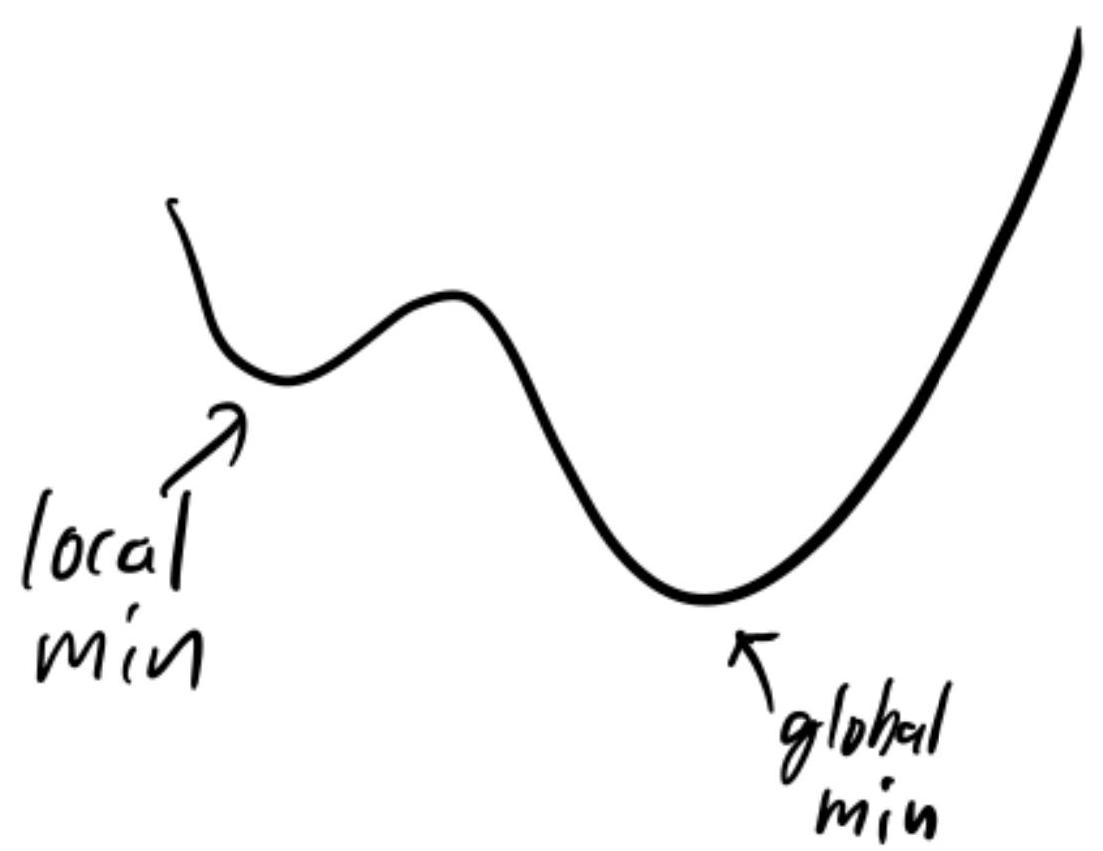
\includegraphics[width=0.5\textwidth]{.././assets/1.1.jpg}
    \end{figure}

    In the worst case, finding the global minimum of an optimization problem is difficult.
    However, in deep learning, optimization problems are often "solved" without any guarantee of global optimality.
\end{definition}

\chapter{Gradient Descent}

\section{Gradient Descent}

\begin{definition}[2.1][Gradient Descent]
    Consider the unconstrained optimization problem

    $$
    \underset{\theta \in \mathbb{R}^{P}}{\operatorname{minimize}} f(\theta)
    $$

    where $f$ is differentiable.

    \textbf{Gradient Descent (GD)} algorithm:

    $$
    \theta^{k+1}=\theta^{k}-\alpha_{k} \nabla f\left(\theta^{k}\right) \quad \text { for } k=0,1, \ldots,
    $$

    where $\theta^{0} \in \mathbb{R}^{p}$ is the \textbf{initial point} and $\alpha_{k}>0$ is the \textbf{learning rate} or the \textbf{stepsize}.

    The terminology learning rate is common in the machine learning literature while stepsize is more common in the optimization literature.
\end{definition}

In math, a function is "differentiable" if its derivative exists everywhere.

In deep learning (DL), a function is often said to be differentiable if its derivative exists almost everywhere and the function is nice.
ReLU activation functions are said to be differentiable.

\begin{concept}[2.2][Efficiency of gradient descent can be expected using the first-order Taylor expansion of $f$.]
    $$
    \theta^{k+1}=\theta^{k}-\alpha_{k} \nabla f\left(\theta^{k}\right)
    $$

    Taylor expansion of $f$ about $\theta^{k}$ :

    $$
    f(\theta)=f\left(\theta^{k}\right)+\nabla f\left(\theta^{k}\right)^{\top}\left(\theta-\theta^{k}\right)+\mathcal{O}\left(\left\|\theta-\theta^{k}\right\|^{2}\right)
    $$

    Plug in $\theta^{k+1}$ :

    $$
    f\left(\theta^{k+1}\right)=f\left(\theta^{k}\right)-\alpha_{k}\left\|\nabla f\left(\theta^{k}\right)\right\|^{2}+\mathcal{O}\left(\alpha_{k}^{2}\right)
    $$

    $-\nabla f\left(\theta^{k}\right)$ is steepest descent direction. For small (cautious) $\alpha_{k}$, GD step reduces function value.
\end{concept}

However, note that a step of GD need not result in descent, i.e., $f\left(\theta^{k+1}\right)>f\left(\theta^{k}\right)$ is possible.

\begin{figure}[H]
    \centering
    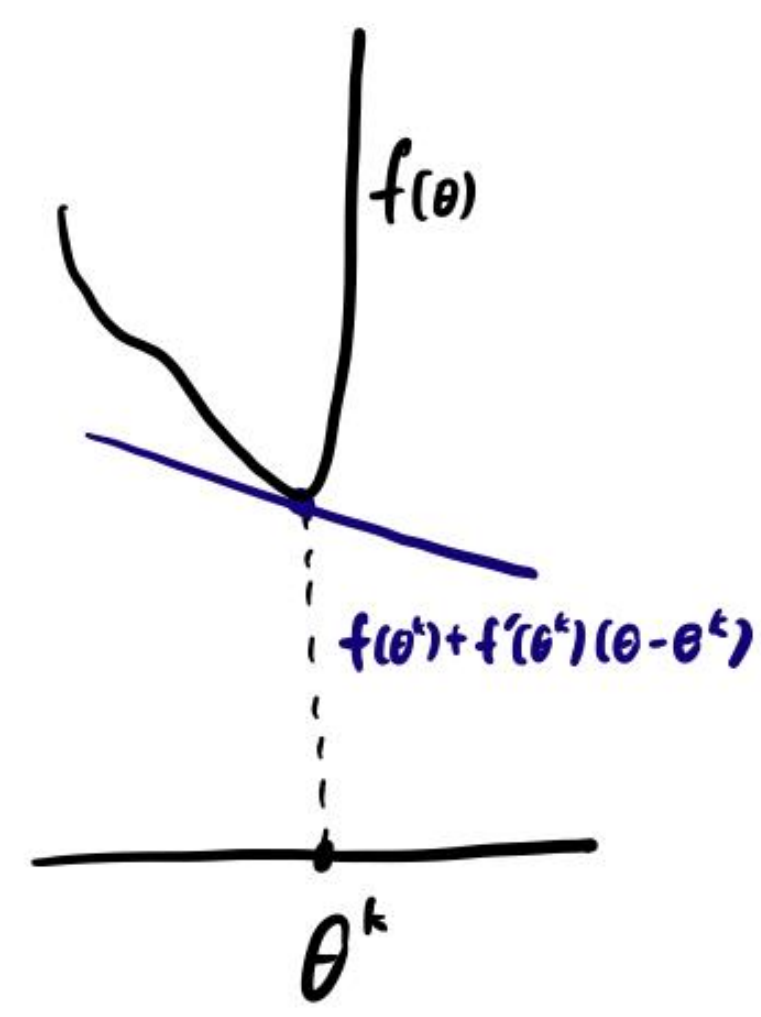
\includegraphics[width=0.4\textwidth]{.././assets/2.1.png}
\end{figure}

We need an assumption that ensures the first-order Taylor expansion is a good approximation within a sufficiently large neighborhood.

\section{Convergence of Gradient Descent}

Without further assumptions, there is no hope of finding the global minimum.

We cannot prove the function value converges to global optimum. We instead prove $\nabla f\left(\theta^{k}\right) \rightarrow 0$. Roughly speaking, this is similar, but weaker than proving that $\theta^{k}$ converges to a local minimum.

\begin{figure}[H]
    \centering
    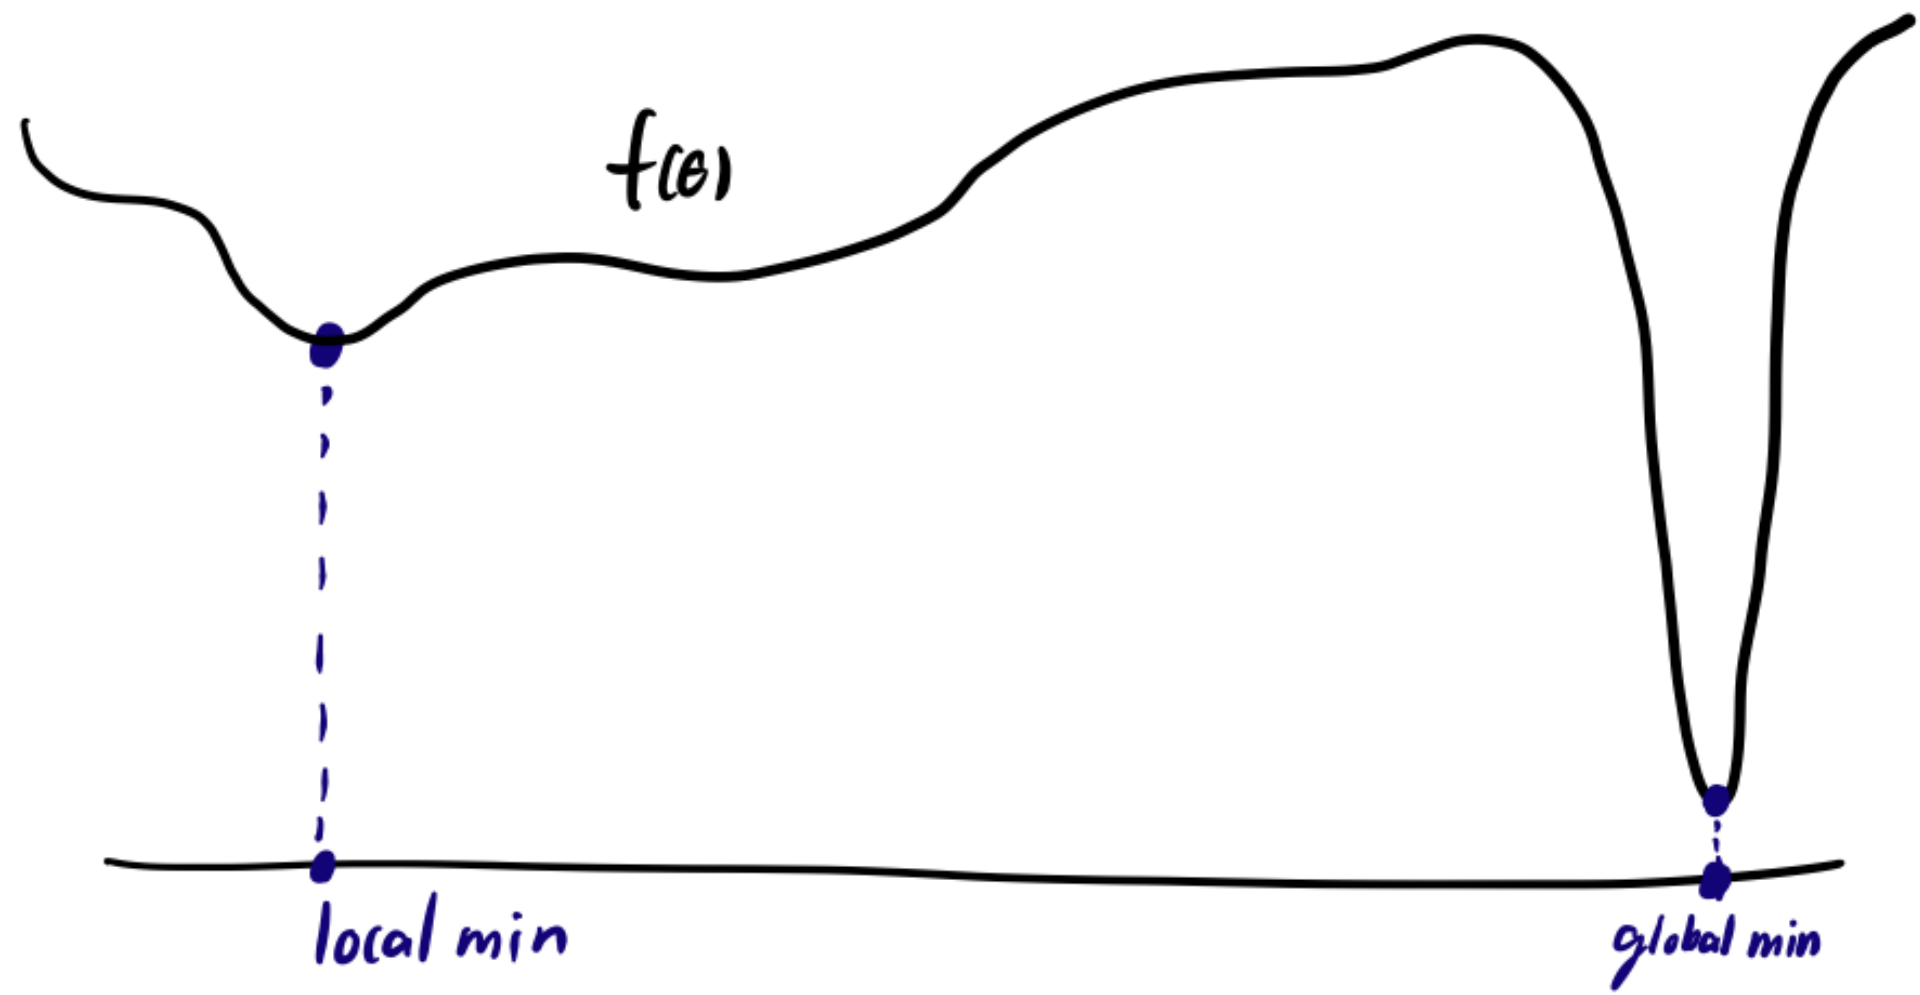
\includegraphics[width=0.7\textwidth]{.././assets/2.2.png}
\end{figure}

Without further assumptions, we cannot show that $\theta^{k}$ converges to a limit, and even $\theta^{k}$ does converge to a limit, we cannot guarantee that that limit is not a saddle point or even a local maximum. Nevertheless, people commonly use the argument that $\theta^{k}$ usually converges and that it is unlikely that the limit is a local maximum or a saddle point.

\begin{definition}[2.3][$L$-Lipschitz]
    We say $\nabla f: \mathbb{R}^{p} \rightarrow \mathbb{R}^{p}$ is $L$-Lipschitz if

    $$
    \|\nabla f(x)-\nabla f(y)\| \leq L\|x-y\| \quad \forall x, y \in \mathbb{R}^{p} .
    $$

    Roughly, this means $\nabla f$ does not change rapidly. As a consequence, we can trust the first-order Taylor expansion on a non-infinitesimal neighborhood.
\end{definition}

\begin{theorem}[2.4][Lipschitz Gradient Lemma]
    Let $f: \mathbb{R}^{p} \rightarrow \mathbb{R}$ be differentiable and $\nabla f: \mathbb{R}^{p} \rightarrow \mathbb{R}^{p}$ be L-Lipschitz. Then

    $$
    f(\theta+\delta) \leq f(\theta)+\nabla f(\theta)^{\top} \delta+\frac{L}{2}\|\delta\|^{2} \quad \forall \theta, \delta \in \mathbb{R}^{p}
    $$

    \par\noindent\textcolor{gray}{\hdashrule{\textwidth}{0.4pt}{1pt 2pt}}

    $f(\theta)+\nabla f(\theta)^{\top} \delta-\frac{L}{2}\|\delta\|^{2} \leq f(\theta+\delta)$ is also true, but we do not need this other direction. Together the inequalities imply

    $$
    \left|f(\theta+\delta)-\left(f(\theta)+\nabla f(\theta)^{\top} \delta\right)\right| \leq \frac{L}{2}\|\delta\|^{2} \quad \forall \theta, \delta \in \mathbb{R}^{p}
    $$

    \begin{proof}
        Define $g: \mathbb{R} \rightarrow \mathbb{R}$ as $g(t)=f(\theta+t \delta)$. Then $g$ is differentiable and

        $$
        g^{\prime}(t)=\nabla f(\theta+t \delta)^{\top} \delta
        $$

        Note $g^{\prime}$ is $\left(L\|\delta\|^{2}\right)$-Lipschitz continuous since

        $$
        \begin{gathered}
        \left|g^{\prime}\left(t_{1}\right)-g^{\prime}\left(t_{0}\right)\right|=\left|\left(\nabla f\left(\theta+t_{1} \delta\right)-\nabla f\left(\theta+t_{0} \delta\right)\right)^{\top} \delta\right| \\
        \leq\left\|\nabla f\left(\theta+t_{1} \delta\right)-\nabla f\left(\theta+t_{0} \delta\right)\right\|\| \| \delta \| \\
        \leq L\left\|t_{1} \delta-t_{0} \delta\right\|\|\delta\| \\
        =L\|\delta\|^{2}\left|t_{1}-t_{0}\right|
        \end{gathered}
        $$

        Finally, we conclude with

        $$
        \begin{gathered}
        f(\theta+\delta)=g(1)=g(0)+\int_{0}^{1} g^{\prime}(t) \mathrm{d} t \\
        \leq f(\theta)+\int_{0}^{1}\left(g^{\prime}(0)+L\|\delta\|^{2} t\right) \mathrm{d} t \\
        =f(\theta)+\nabla f(\theta)^{\top} \delta+\frac{L}{2}\|\delta\|^{2}
        \end{gathered}
        $$
    \end{proof}
\end{theorem}

\begin{theorem}[2.5][Summability Lemma]
    Let $V^{0}, V^{1}, \ldots \in \mathbb{R}$ and $S^{0}, S^{1}, \ldots \in \mathbb{R}$ be nonnegative sequences satisfying

    $$
    V^{k+1} \leq V^{k}-S^{k}
    $$

    for $k=0,1,2, \ldots$ Then $S^{k} \rightarrow 0$.

    \begin{proof}
        Key idea. $S^{k}$ measures progress (decrease) made in iteration $k$. Since $V^{k} \geq 0, V^{k}$ cannot decrease forever, so the progress (magnitude of $S^{k}$ ) must diminish to 0.

        Sum the inequality from $i=0$ to $k$

        $$
        V^{k+1}+\sum_{i=0}^{k} S^{i} \leq V^{0}
        $$

        Let $k \rightarrow \infty$

        $$
        \sum_{i=0}^{\infty} S^{i} \leq V^{0}-\lim _{k \rightarrow \infty} V^{k} \leq V^{0}
        $$

        Since $\sum_{i=0}^{\infty} S^{i}<\infty, S^{i} \rightarrow 0$.
    \end{proof}
\end{theorem}

\begin{theorem}[2.6][Convergence of GD]
    Assume $f: \mathbb{R}^{p} \rightarrow \mathbb{R}$ is differentiable, $\nabla f$ is $L$-Lipschitz continuous, and $\inf _{\theta \in \mathbb{R}^{p}} f(\theta)>-\infty$. Then

    $$
    \theta^{k+1}=\theta^{k}-\alpha \nabla f\left(\theta^{k}\right)
    $$

    with $\alpha \in\left(0, \frac{2}{L}\right)$ satisfies $\nabla f\left(\theta^{k}\right) \rightarrow 0$.

    \begin{proof}
        Use Lipschitz gradient lemma with $\theta=\theta^{k}$ and $\delta=-\alpha \nabla f\left(\theta^{k}\right)$ to get

        $$
        f\left(\theta^{k+1}\right) \leq f\left(\theta^{k}\right)-\alpha\left(1-\frac{\alpha L}{2}\right)\left\|\nabla f\left(\theta^{k}\right)\right\|^{2}
        $$

        and

        $$
        \left(f\left(\theta^{k+1}\right)-\inf _{\theta} f(\theta)\right) \leq\left(f\left(\theta^{k}\right)-\inf _{\theta} f(\theta)\right)-\alpha\left(1-\frac{\alpha L}{2}\right)\left\|\nabla f\left(\theta^{k}\right)\right\|^{2} \\
        $$

        $$
        \left(f\left(\theta^{k+1}\right)-\inf _{\theta} f(\theta)\right) \ge 0, 
        \left(f\left(\theta^{k}\right)-\inf _{\theta} f(\theta)\right) \ge 0, 
        \alpha\left(1-\frac{\alpha L}{2}\right)\left\|\nabla f\left(\theta^{k}\right)\right\|^{2} > 0 \text{ for } \alpha \in\left(0, \frac{2}{L}\right)
        $$

        By the summability lemma, $\left\|\nabla f\left(\theta^{k}\right)\right\|^{2} \rightarrow 0$ and thus $\nabla f\left(\theta^{k}\right) \rightarrow 0$.
    \end{proof}
\end{theorem}

In deep learning, the condition that $\nabla f$ is $L$-Lipschitz is usually not true (due to the use of ReLU activation functions).

Rather, the purpose of these mathematical analyses is to obtain qualitative insights; this convergence proof are meant to provide you with intuition on the training dynamics of GD and SGD.

Because analyzing deep learning systems as is rigorously is usually difficult, people usually analyze modified (simplified) setups rigorously or analyze the full setup heuristically.

In both cases, the goal is to obtain qualitative insights, rather than theoretical guarantees.

\section{Stochastic Gradient Descent}

\begin{definition}[2.7][Finite-Sum Optimization Problem]
    A \textbf{finite-sum optimization problem} has the structure

    $$
    \underset{\theta \in \mathbb{R}^{p}}{\operatorname{minimize}} \frac{1}{N} \sum_{i=1}^{N} f_{i}(\theta):=F(\theta)
    $$

    Finite-sum is ubiquitous in ML. $N$ usually corresponds to the number of data points.
\end{definition}

In finite-sum problem, using GD

$$
\theta^{k+1}=\theta^{k}-\frac{\alpha_{k}}{N} \sum_{i=1}^{N} \nabla f_{i}\left(\theta^{k}\right)
$$

is impractical when $N$ is large since $\frac{1}{N} \sum_{i=1}^{N} \nabla f_{i}\left(\theta^{k}\right)$ takes too long to compute.

\begin{concept}[2.8][Finite-sum problem can be reformulated with expectation.]
    Although the finite-sum optimization problem has no inherent randomness, we can reformulate this problem with randomness:

    $$
    \operatorname{minimize}_{\theta \in \mathbb{R}^{p}} \quad \mathbb{E}_{I}\left[f_{I}(\theta)\right]
    $$

    where $I \sim$ Uniform $\{1, \ldots, N\}$. To see the equivalence,

    $$
    \mathbb{E}_{I}\left[f_{I}(\theta)\right]=\sum_{i=1}^{N} f_{i}(\theta) \mathbb{P}(I=i)=\frac{1}{N} \sum_{i=1}^{N} f_{i}(\theta)=F(\theta)
    $$
\end{concept}

\begin{definition}[2.9][Stochastic Gradient Descent]
    \textbf{Stochastic gradient descent (SGD)}

    $$
    \begin{gathered}
    i(k) \sim \operatorname{Uniform}\{1, \ldots, N\} \\
    \theta^{k+1}=\theta^{k}-\alpha_{k} \nabla f_{i(k)}\left(\theta^{k}\right)
    \end{gathered}
    $$

    for $k=0,1, \ldots$, where $\theta^{0} \in \mathbb{R}^{p}$ is the \textbf{initial point} and $\alpha_{k}>0$ is the \textbf{learning rate}.

    $\nabla f_{i(k)}\left(\theta^{k}\right)$ is a stochastic gradient of $F$ at $\theta^{k}$, i.e.,

    $$
    \mathbb{E}\left[\nabla f_{i(k)}\left(\theta^{k}\right)\right]=\nabla \mathbb{E}\left[f_{i(k)}\left(\theta^{k}\right)\right]=\nabla F\left(\theta^{k}\right)
    $$
\end{definition}

\begin{concept}[2.10][SGD is more efficient than GD.]
    GD uses all indices $i=1, \ldots, N$ every iteration

    $$
    \theta^{k+1}=\theta^{k}-\frac{\alpha_{k}}{N} \sum_{i=1}^{N} \nabla f_{i}\left(\theta^{k}\right)
    $$

    SGD uses only a single random index $i(k)$ every iteration

    $$
    \begin{gathered}
    i(k) \sim \text { Uniform }\{1, \ldots, N\} \\
    \theta^{k+1}=\theta^{k}-\alpha_{k} \nabla f_{i(k)}\left(\theta^{k}\right)
    \end{gathered}
    $$

    When size of the data $N$ is large, SGD is often more effective than GD.
\end{concept}

\begin{concept}[2.11][Efficiency of stochastic gradient descent can be expected using the first-order Taylor expansion of $F$.]
    Plug $\theta^{k+1}$ into Taylor expansion of $F$ about $\theta^{k}$ :

    $$
    F\left(\theta^{k+1}\right)=F\left(\theta^{k}\right)-\alpha_{k} \nabla F\left(\theta^{k}\right)^{\top} \nabla f_{i(k)}\left(\theta^{k}\right)+\mathcal{O}\left(\alpha_{k}^{2}\right)
    $$

    Take expectation on both sides:

    $$
    \mathbb{E}_{k}\left[F\left(\theta^{k+1}\right)\right]=F\left(\theta^{k}\right)-\alpha_{k}\left\|\nabla F\left(\theta^{k}\right)\right\|^{2}+\mathcal{O}\left(\alpha_{k}^{2}\right)
    $$

    ( $\mathbb{E}_{k}$ is expectation conditioned on $\theta^{k}$ )

    $-\nabla f_{i(k)}\left(\theta^{k}\right)$ is descent direction in expectation. For small (cautious) $\alpha_{k}$, SGD step reduces function value in expectation.
\end{concept}

\section{Variants of Stochastic Gradient Descent}

Consider

$$
\underset{\theta \in \mathbb{R}^{p}}{\operatorname{minimize}} \frac{1}{N} \sum_{i=1}^{N} f_{i}(\theta)
$$

SGD can be generalized to

$$
\theta^{k+1}=\theta^{k}-\alpha_{k} g^{k}
$$

where $g^{k}$ is a stochastic gradient. The choice $g^{k}=\nabla f_{i(k)}\left(\theta^{k}\right)$ is just one option.

\begin{theorem}[2.12][Sampling with Replacement Lemma]
    Let $X_{1}, \ldots, X_{N} \in \mathbb{R}^{p}$ be given (non-random) vectors. Let $\frac{1}{N} \sum_{i=1}^{N} X_{i}=\mu$. Let $i(1), \ldots, i(B) \subseteq\{1, \ldots, N\}$ be random indices. Then

    $$
    \mathbb{E} \frac{1}{B} \sum_{b=1}^{B} X_{i(b)}=\mu
    $$

    \begin{proof}
        $$
        \mathbb{E} \frac{1}{B} \sum_{b=1}^{B} X_{i(b)}=\frac{1}{B} \sum_{b=1}^{B} \mathbb{E} X_{i(b)}=\frac{1}{B} \sum_{b=1}^{B} \mu=\mu
        $$
    \end{proof}
\end{theorem}

\begin{definition}[2.13][Minibatch SGD with Replacement]
    \textbf{Minibatch SGD with replacement}

    $$
    \begin{gathered}
    i(k, 1), \ldots, i(k, B) \sim \text { Uniform }\{1, \ldots, N\} \\
    \theta^{k+1}=\theta^{k}-\frac{\alpha_{k}}{B} \sum_{b=1}^{B} \nabla f_{i(k, b)}\left(\theta^{k}\right)
    \end{gathered}
    $$

    To clarify, we sample $B$ out of $N$ indices with replacement, i.e., the same index can be sampled multiple times.

    By \hyperref[theorem:2.12]{Theorem 2.12}, $\frac{1}{B} \sum_{b=1}^{B} \nabla f_{i(k, b)}\left(\theta^{k}\right)$ is a stochastic gradient of $F$ at $\theta^{k}$.
\end{definition}

\begin{theorem}[2.14][Sampling without Replacement Lemma]
    Let $X_{1}, \ldots, X_{N} \in \mathbb{R}^{p}$ be given (non-random) vectors. Let $\frac{1}{N} \sum_{i=1}^{N} X_{i}=\mu$. Let $\sigma$ be a random permutation. Then

    $$
    \mathbb{E} \frac{1}{B} \sum_{b=1}^{B} X_{\sigma(b)}=\mu
    $$

    \begin{proof}
        $$
        \mathbb{E} \frac{1}{B} \sum_{b=1}^{B} X_{\sigma(b)}=\frac{1}{B} \sum_{b=1}^{B} \mathbb{E} X_{\sigma(b)}=\frac{1}{B} \sum_{b=1}^{B} \mu=\mu
        $$
    \end{proof}
\end{theorem}

\begin{definition}[2.15][Minibatch SGD without Replacement]
    \textbf{Minibatch SGD without replacement}

    $$
    \begin{gathered}
    \sigma^{k} \sim \operatorname{permutation}(N) \\
    \theta^{k+1}=\theta^{k}-\frac{\alpha_{k}}{B} \sum_{b=1}^{B} \nabla f_{\sigma^{k}(b)}\left(\theta^{k}\right)
    \end{gathered}
    $$

    We assume $B \leq N$. To clarify, we sample $B$ out of $N$ indices without replacement, i.e., the same index cannot be sampled multiple times.

    By \hyperref[theorem:2.14]{Theorem 2.14}, $\frac{1}{B} \sum_{b=1}^{B} \nabla f_{\sigma^{k}(b)}\left(\theta^{k}\right)$ is a stochastic gradient of $F$ at $\theta^{k}$.
\end{definition}

\begin{concept}[2.16][How to choose batch size $B$?]
    Note $B=1$ minibatch SGD becomes SGD.

    Mathematically (measuring performance per iteration)

    \begin{itemize}
        \item Use large batch is when noise/randomness is large.
        \item Use small batch is when noise/randomness is small.
    \end{itemize}

    Practically (measuring performance per unit time)

    \begin{itemize}
        \item Large batch allows more efficient computation on GPUs.
        \item Often best to increase batch size up to the GPU memory limit.
    \end{itemize}
\end{concept}

In DL, SGD is applied to nice continuous but non-differentiable functions that are differentiable almost everywhere.

In this case, if we choose $\theta^{0} \in \mathbb{R}^{n}$ randomly and run

$$
\theta^{k+1}=\theta^{k}-\alpha_{k} \nabla f\left(\theta^{k}\right)
$$

the algorithm is usually well-defined, i.e., $\theta^{k}$ never hits a point of non-differentiability.

With a proof or not, GD and SGD are applied to non-differentiable minimization in ML. The absence of differentiability does not seem to cause serious problems.

\begin{definition}[2.17][Cyclic SGD]
    Consider the sequence of indices

    $$
    \{\bmod (k, N)+1\}_{k=0,1, \ldots}=1,2, \ldots, N, 1,2, \ldots, N, \ldots
    $$

    Here, $\bmod (k, N)$ is the remainder of $k$ when divided by $N$.

    \textbf{Cyclic SGD}:

    $$
    \theta^{k+1}=\theta^{k}-\alpha_{\mathbf{k}} \nabla f_{\bmod (k, N)+1}\left(\theta^{k}\right)
    $$

    To clarify, this samples the indices in a (deterministic) cyclic order.
\end{definition}

\begin{concept}[2.18][Pros and Cons of Cyclic SGD]
    Strictly speaking, cyclic SGD is not an instance of SGD as unbiased estimation property lost.

    Advantage:

    \begin{itemize}
        \item Uses all indices (data) every $N$ iterations.
    \end{itemize}

    Disadvantage:

    \begin{itemize}
        \item Worse than SGD in some cases, theoretically and empirically.
        \item In DL, neural networks can learn to anticipate cyclic order.
    \end{itemize}
\end{concept}

\begin{definition}[2.19][Shuffled Cyclic SGD]
    \textbf{Shuffled Cyclic SGD}:

    $$
    \theta^{k+1}=\theta^{k}-\alpha_{k} \nabla f_{\sigma^{\left \lfloor \frac{k}{N} \right \rfloor} (\bmod (k, N)+1)}\left(\theta^{k}\right)
    $$

    where $\sigma^{0}, \sigma^{1}, \ldots$ is a sequence of random permutations, i.e., we shuffle the order every cycle.
\end{definition}

\begin{concept}[2.19][Pros and Cons of Shuffled Cyclic SGD]
    Again, strictly speaking, shuffled cyclic SGD is not an instance of SGD as unbiased estimation property lost.

    Advantages :

    \begin{itemize}
        \item Uses all indices (data) every $N$ iterations.
        \item Neural network cannot learn to anticipate data order.
        \item Empirically best performance.
    \end{itemize}

    Disadvantages:

    \begin{itemize}
        \item Theory not as strong as regular SGD.
    \end{itemize}
\end{concept}

\begin{concept}[2.20][Which variant of SGD to use?]
    Theoretical comparison of SGD variants:

    \begin{itemize}
        \item Not that easy.
        \item Result does not strongly correlate with practical performance in DL.
    \end{itemize}

    In DL, the most common choice is

    \begin{itemize}
        \item shuffled cyclic minibatch SGD (without replacement) and
        \item batchsize $B$ is as large as possible within the GPU memory limit.
    \end{itemize}

    One can generally consider this to be the default option.
\end{concept}

\begin{definition}[2.21][Epoch in finite-sum optimization and machine learning training]
    An \textbf{epoch} is loosely defined as the unit of optimization or training progress of processing all indices or data once.

    \begin{itemize}
        \item 1 iteration of GD constitutes an epoch.
        \item $N$ iterations of SGD, cyclic SGD, or shuffled cyclic SGD constitute an epoch.
        \item $N / B$ iterations of minibatch SGD constitute an epoch.
    \end{itemize}

    Epoch is often a convenient unit for counting iterations compared to directly counting the iteration number.
\end{definition}

\begin{concept}[2.22][SGD with General Expectation]
    Consider an optimization problem with its objective defined with a general expectation

    $$
    \operatorname{minimize}_{\theta \in \mathbb{R}^{p}} \quad \mathbb{E}_{\omega}\left[f_{\omega}(\theta)\right]:=F(\theta)
    $$

    Here, $\omega$ is a random variable. We will encounter these expectations (non-finite sum) when we talk about generative models.

    For this setup, the SGD algorithm is

    $$
    \theta^{k+1}=\theta^{k}-\alpha_{k} \nabla f_{\omega^{k}}\left(\theta^{k}\right)
    $$

    where $\omega^{0}, \omega^{1}, \ldots$ are IID random samples of $\omega$. If $\nabla_{\theta} \mathbb{E}_{\omega}\left[f_{\omega}(\theta)\right]=\mathbb{E}_{\omega}\left[\nabla_{\theta} f_{\omega}(\theta)\right]$, then $\nabla f_{\omega^{k}}\left(\theta^{k}\right)$ is a stochastic gradient of $F(\theta)$ at $\theta^{k}$. (Make sure you understand why the previous SGD for the finite-sum setup is a special case of this.)

    GD for this setup is

    $$
    \theta^{k+1}=\theta^{k}-\alpha_{k} \mathbb{E}_{\omega}\left[\nabla_{\theta} f_{\omega}\left(\theta^{k}\right)\right]
    $$

    However, if the expectation is difficult to compute GD is impractical and SGD is preferred.
\end{concept}

\chapter*{Chapter 1 Code}

\href{https://drive.google.com/file/d/1PSpoeseUPIptYQOPuQpxNawxtZbVR_K6/view?usp=sharing}{Chapter 1 Code}

\part{Shallow Neural Networks to Multilayer Perceptrons}

\chapter{Shallow Neural Networks}

\section{Supervised Learning Problem}

\begin{definition}[3.1][Supervised Learning Setup]
    We have data $X_{1}, \ldots, X_{N} \in \mathcal{X}$ and corresponding labels $Y_{1}, \ldots, Y_{N} \in \mathcal{Y}$.

    \begin{itemize}
        \item Example) $X_{i}$ is the $i$ th email and $Y_{i} \in\{-1,+1\}$ denotes whether $X_{i}$ is a spam email.
        \item Example) $X_{i}$ is the $i$ th image and $Y_{i} \in\{0, \ldots, 9\}$ denotes handwritten digit.
    \end{itemize}

    Assume there is a true unknown function

    $$
    f_{\star}: x \rightarrow y
    $$

    mapping data to its label. In particular, $Y_{i}=f_{\star}\left(X_{i}\right)$ for $i=1, \ldots, N$.

    The goal of supervised learning is to use $X_{1}, \ldots, X_{N}$ and $Y_{1}, \ldots, Y_{N}$ to find $f \approx f_{\star}$.
\end{definition}

\begin{definition}[3.2][Supervised Learning Objective]
    Assume a loss function such that $\ell\left(y_{1}, y_{2}\right)=0$ if $y_{1}=y_{2}$ and $\ell\left(y_{1}, y_{2}\right)>0$ if $y_{1} \neq y_{2}$.

    Restrict search to a class of parametrized functions $f_{\theta}(x)$ where $\theta \in \Theta \subseteq \mathbb{R}^{p}$, i.e., only consider $f \in\left\{f_{\theta} \mid \theta \in \Theta\right\}$ where $\Theta \subseteq \mathbb{R}^{p}$.

    Take a finite sample $X_{1}, \ldots, X_{N} \in \mathcal{X}$ and corresponding labels $Y_{1}, \ldots, Y_{N} \in \mathcal{Y}$. Then solve

    $$
    \underset{\theta \in \Theta}{\operatorname{minimize}} \frac{1}{N} \sum_{i=1}^{N} \ell\left(f_{\theta}\left(X_{i}\right), f_{\star}\left(X_{i}\right)\right)
    $$

    which is equivalent to

    $$
    \underset{\theta \in \Theta}{\operatorname{minimize}} \frac{1}{N} \sum_{i=1}^{N} \ell\left(f_{\theta}\left(X_{i}\right), Y_{i}\right)
    $$

    This is the standard form of the optimization problem (except regularizers) we consider in the supervised learning. We will talk about regularizers later.
\end{definition}

\begin{concept}[3.3][Training is optimization.]
    In machine learning, the anthropomorphized word "\textbf{training}" refers to solving an optimization problem such as

    $$
    \underset{\theta \in \Theta}{\operatorname{minimize}} \frac{1}{N} \sum_{i=1}^{N} \ell\left(f_{\theta}\left(X_{i}\right), Y_{i}\right)
    $$

    In most cases, SGD or variants of SGD are used.

    We call $f_{\theta}$ the \textbf{machine learning model} or the \textbf{neural network}.
\end{concept}

\begin{example}[3.4][Least-Squares Regression]
    In LS, $\mathcal{X}=\mathbb{R}^{p}, \mathcal{Y}=\mathbb{R}, \Theta=\mathbb{R}^{p}, f_{\theta}(x)=x^{\top} \theta$, and $\ell\left(y_{1}, y_{2}\right)=\frac{1}{2}\left(y_{1}-y_{2}\right)^{2}$.

    So we solve

    $$
    \underset{\theta \in \mathbb{R}^{p}}{\operatorname{minimize}} \frac{1}{N} \sum_{i=1}^{N} \frac{1}{2}\left(f_{\theta}\left(X_{i}\right)-Y_{i}\right)^{2}=\frac{1}{N} \sum_{i=1}^{N} \frac{1}{2}\left(X_{i}^{\top} \theta-Y_{i}\right)^{2}=\frac{1}{2 N}\|X \theta-Y\|^{2}
    $$

    where $X=\left[\begin{array}{c}X_{1}^{\top} \\ \vdots \\ X_{N}^{\top}\end{array}\right]$ and $Y=\left[\begin{array}{c}Y_{1} \\ \vdots \\ Y_{N}\end{array}\right]$.

    The model $f_{\theta}(x)=x^{\top} \theta$ is a shallow neural network. (The terminology will makes sense when contrasted with deep neural networks.)
\end{example}

\section{Linear Classification}

\begin{definition}[3.5][Binary Classification and Linear Separability]
    In \textbf{binary classification}, we have $\mathcal{X}=\mathbb{R}^{p}$ and $\mathcal{Y}=\{-1,+1\}$.

    The data is \textbf{linearly separable} if there is a hyperplane defined by $(a_{\text {true }}, b_{\text {true }} )$ such that

    $$
    y=\left\{\begin{array}{cl}
    1 & \text { if } a_{\text {true }}^{\top} x+b_{\text {true }}>0 \\
    -1 & \text { otherwise. }
    \end{array}\right.
    $$

    \begin{figure}[H]
        \centering
        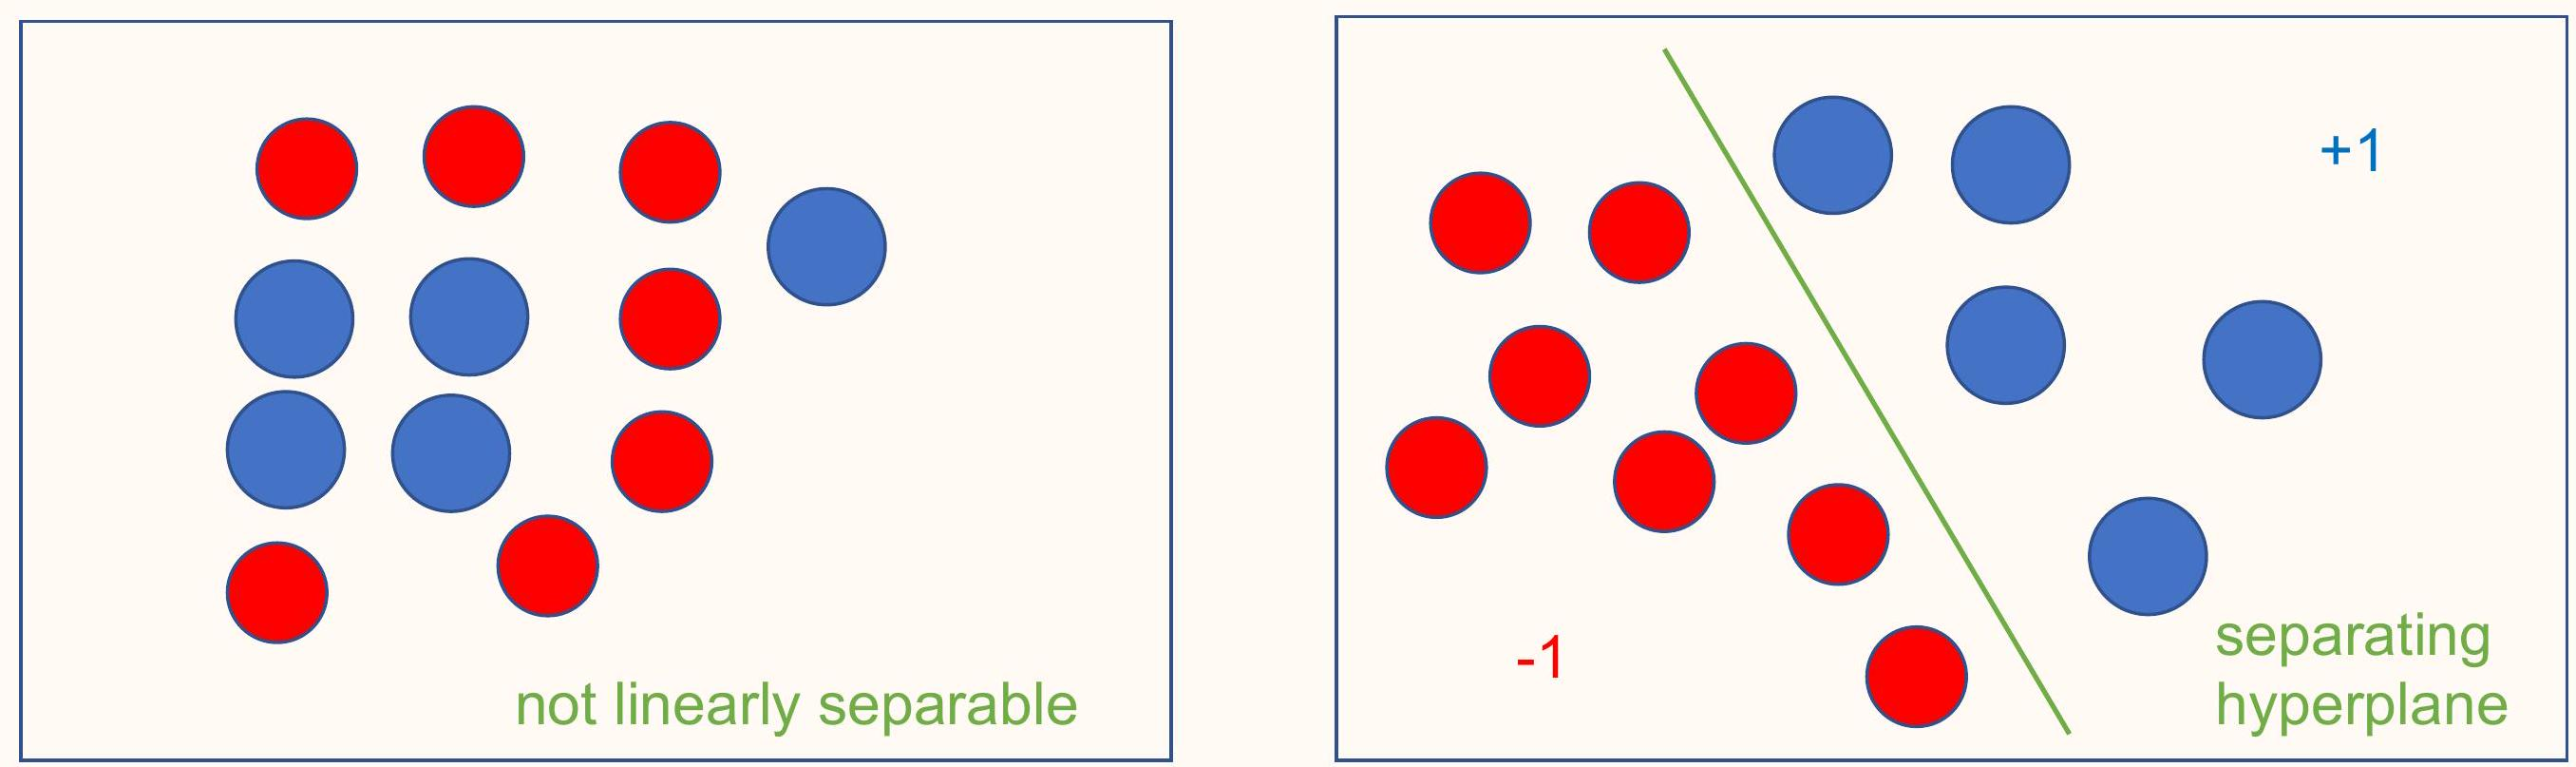
\includegraphics[width=1.0\textwidth]{.././assets/3.1.jpg}
    \end{figure}
\end{definition}

\subsection{Support Vector Machine   }

Consider linear (affine) models

$$
f_{a, b}(x)= \begin{cases}+1 & \text { if } a^{\top} x+b>0 \\ -1 & \text { otherwise }\end{cases}
$$

Consider the loss function

$$
\ell\left(y_{1}, y_{2}\right)=\frac{1}{2}\left|1-y_{1} y_{2}\right|= \begin{cases}0 & \text { if } y_{1}=y_{2} \\ 1 & \text { if } y_{1} \neq y_{2}\end{cases}
$$

The optimization problem

$$
\underset{a \in \mathbb{R}^{p}, b \in \mathbb{R}}{\operatorname{minimize}} \frac{1}{N} \sum_{i=1}^{N} \ell\left(f_{a, b}\left(X_{i}\right), Y_{i}\right)
$$

has a solution with optimal value 0 when the data is linearly separable.

Problem: Optimization problem is discontinuous and thus cannot be solved with SGD.

\par\noindent\textcolor{gray}{\hdashrule{\textwidth}{0.4pt}{1pt 2pt}}

\textbf{Motivation for SVM}

Even if the underlying function or phenomenon to approximate is discontinuous, the model needs to be continuous in its parameters. The loss function also needs to be continuous. (The prediction need not be continuous.)

We consider a relaxation, is a continuous proxy of the discontinuous thing. Specifically, consider

$$
f_{a, b}(x)=a^{\top} x+b
$$

Once trained, $f_{a, b}(x)>0$ means the neural network is predicting $y=+1$ to be "more likely", and $f_{a, b}(x)<0$ means the neural network is predicting $y=-1$ to be "more likely".

Therefore, we train the model to satisfy

$$
Y_{i} f_{a, b}\left(X_{i}\right)>0 \text { for } i=1, \ldots, N .
$$

Problem with strict inequality $Y_{i} f_{a, b}\left(X_{i}\right)>0$ :

\begin{itemize}
    \item Strict inequality has numerical problems with round-off error.
    \item The magnitude $\left|f_{a, b}(x)\right|$ can be viewed as the confidence of the prediction, but having a small positive value for $Y_{i} f_{a, b}\left(X_{i}\right)$ indicates small confidence of the neural network.
\end{itemize}

We modify our model's desired goal to be $Y_{i} f_{a, b}\left(X_{i}\right) \geq 1$.

To train the neural network to satisfy

$$
0 \geq 1-Y_{i} f_{a, b}\left(X_{i}\right) \text { for } i=1, \ldots, N .
$$

we minimize the excess positive component of the RHS

$$
\underset{a \in \mathbb{R}^{p}, b \in \mathbb{R}}{\operatorname{minimize}} \frac{1}{N} \sum_{i=1}^{N} \max \left\{0,1-Y_{i} f_{a, b}\left(X_{i}\right)\right\}
$$

which is equivalent to

$$
\underset{a \in \mathbb{R}^{p}, b \in \mathbb{R}}{\operatorname{minimize}} \frac{1}{N} \sum_{i=1}^{N} \max \left\{0,1-Y_{i}\left(a^{\top} X_{i}+b\right)\right\}
$$

If the optimal value is 0, then the data is linearly separable.

\begin{definition}[3.6][Support Vector Machine (SVM)]
    Use the model

    $$
    f_{a, b}(x)=a^{\top} x+b
    $$

    This following formulation is called the \textbf{support vector machine (SVM)}

    $$
    \underset{a \in \mathbb{R}^{p}, b \in \mathbb{R}}{\operatorname{minimize}} \frac{1}{N} \sum_{i=1}^{N} \max \left\{0,1-Y_{i} f_{a, b}\left(X_{i}\right)\right\}
    $$

    $$
    \underset{a \in \mathbb{R}^{p}, b \in \mathbb{R}}{\operatorname{minimize}} \frac{1}{N} \sum_{i=1}^{N} \max \left\{0,1-Y_{i}\left(a^{\top} X_{i}+b\right)\right\}
    $$

    It is also common to add a regularizer

    $$
    \underset{a \in \mathbb{R}^{p}, b \in \mathbb{R}}{\operatorname{minimize}} \frac{1}{N} \sum_{i=1}^{N} \max \left\{0,1-Y_{i}\left(a^{\top} X_{i}+b\right)\right\}+\frac{\lambda}{2}\|a\|^{2}
    $$
\end{definition}

\begin{concept}[3.7][Prediction with SVM]
    Once the SVM is trained, make predictions with

    $$
    \operatorname{sign}\left(f_{a, b}(x)\right)=\operatorname{sign}\left(a^{\top} x+b\right)
    $$

    when $f_{a, b}(x)=0$, we assign $\operatorname{sign}\left(f_{a, b}(x)\right)$ arbitrarily.

    Note that the prediction is discontinuous, but predictions are in $\{-1,+1\}$ so it must be discontinuous.

    If $\sum_{i=1}^{N} \max \left\{0,1-Y_{i} f_{a, b}\left(X_{i}\right)\right\}=0$, then $\operatorname{sign}\left(f_{a, b}\left(X_{i}\right)\right)=Y_{i}$ for $i=1, \ldots, N$, i.e., the neural network predicts the known labels perfectly.
    Of course, it is a priori not clear how accurate the prediction will be for new unseen data.
\end{concept}

\subsection{Logistic Regression}

\begin{concept}[3.8][Relaxed Supervised Learning Setup]
    We relax the supervised learning setup to predict probabilities, rather than make point predictions.
    So, labels are generated based on data, perhaps randomly.
    Consider data $X_{1}, \ldots, X_{N} \in \mathcal{X}$ and labels $Y_{1}, \ldots, Y_{N} \in \mathcal{Y}$. Assume there exists a function

    $$
    f_{\star}: \mathcal{X} \rightarrow \mathcal{P}(\mathcal{Y})
    $$

    where $\mathcal{P}(\mathcal{Y})$ denotes the set of probability distributions on $\mathcal{Y}$.
    Assume the generation of $Y_{i}$ given $X_{i}$ is independent of $Y_{j}$ and $X_{j}$ for $j \neq i$.

    \begin{itemize}
        \item Example) $f(X)=\left[\begin{array}{l}0.8 \\ 0.2\end{array}\right]$ in dog vs. cat classifier.
        \item Example) An email saying "Buy this thing at our store!" may be spam to some people, but it may not be spam to others.
    \end{itemize}

    The relaxed SL setup is more general and further realistic.
\end{concept}

\begin{definition}[3.9][Empirical Distribution for Binary Classification]
    In basic binary classification, define the \textbf{empirical distribution}

    $$
    \mathcal{P}(y)= \begin{cases}{\left[\begin{array}{l}
    1 \\
    0
    \end{array}\right]} & \text { if } y=-1 \\
    {\left[\begin{array}{l}
    0 \\
    1
    \end{array}\right]} & \text { if } y=+1\end{cases}
    $$

    More generally, the \textbf{empirical distribution} describes the data we have seen.
    In this context, we have only seen one label per datapoint, so our empirical distributions are one-hot vectors.

    (If there are multiple annotations per data point $x$ and they don't agree, then the empirical distribution may not be one-hot vectors.
    For example, given the same email, some users may flag it as spam while others consider it useful information.)
\end{definition}

\begin{definition}[3.10][KL-Divergence, Cross Entropy]
    Let $p, q \in \mathbb{R}^{n}$ represent probability masses, i.e., $p_{i} \geq 0$ for $i=1, \ldots, n$ and $\sum_{i=1}^{n} p_{i}=1$ and the same for $q$.
    The \textbf{Kullback-Leibler-divergence (KL-divergence)} from $q$ to $p$ is

    $$
    \begin{array}{ll}
    D_{\mathrm{KL}}(p \| q)=\displaystyle \sum_{i=1}^{n} p_{i} \log \left(\frac{p_{i}}{q_{i}}\right)= & -\displaystyle \sum_{i=1}^{n} p_{i} \log \left(q_{i}\right) & +\displaystyle \sum_{i=1}^{n} p_{i} \log \left(p_{i}\right) \\
    & =H(p, q) & =-H(p) \\
    & \text { cross entropy of } q & =-H \\
    & \text { relative to } p & \text { entropy of } p
    \end{array}
    $$

    The \textbf{cross entropy of $q$ relative to $p$} is

    $$
    H(p, q) = -\sum_{i=1}^{n} p_{i} \log \left(q_{i}\right)
    $$
\end{definition}

\begin{theorem}[3.11][Properties of KL-Divergence]
    $$
    D_{\mathrm{KL}}(p \| q)=\sum_{i=1}^{n} p_{i} \log \left(\frac{p_{i}}{q_{i}}\right)
    $$

    \begin{itemize}
        \item Not symmetric, i.e., $D_{\mathrm{KL}}(p \| q) \neq D_{\mathrm{KL}}(q \| p)$.
        \item $D_{\mathrm{KL}}(p \| q)>0$ if $p \neq q$ and $D_{\mathrm{KL}}(p \| q)=0$ if $p=q$.
        \item $D_{\mathrm{KL}}(p \| q)=\infty$ is possible. (Further detail below.)
    \end{itemize}

    Often used as a "distance" between $p$ and $q$ despite not being a metric.

    \par\noindent\textcolor{gray}{\hdashrule{\textwidth}{0.4pt}{1pt 2pt}}

    Clarification: Use the convention

    \begin{itemize}
        \item $0 \log \left(\frac{0}{0}\right)=0\left(\right.$ when $\left.p_{i}=q_{i}=0\right)$
        \item $0 \log \left(\frac{0}{q_{i}}\right)=0$ if $q_{i}>0$
        \item $p_{i} \log \left(\frac{p_{i}}{0}\right)=\infty$ if $p_{i}>0$
    \end{itemize}

    \par\noindent\textcolor{gray}{\hdashrule{\textwidth}{0.4pt}{1pt 2pt}}

    Probabilistic interpretation:

    $$
    D_{\mathrm{KL}}(p \| q)=\mathbb{E}_{I}\left[\log \left(\frac{p_{I}}{q_{I}}\right)\right]
    $$

    with the random variable $I$ such that $\mathbb{P}(I=i)=p_{i}$.
\end{theorem}

\begin{definition}[3.12][Logistic Regression (LR)]
    \textbf{Logistic regression (LR)}, is another model for binary classification:

    Use the model

    $$
    f_{a, b}(x)=\left[\begin{array}{c}
    \frac{1}{1+e^{a^{\top} x+b}} \\
    \frac{e^{a^{\top} x+b}}{1+e^{a^{\top} x+b}}
    \end{array}\right]=\left[\begin{array}{c}
    \frac{1}{1+e^{a^{\top} x+b}} \\
    \frac{1}{1+e^{-\left(a^{\top} x+b\right)}}
    \end{array}\right]\begin{array}{c}
    = \mathbb{P}(y=-1) \\
    = \mathbb{P}(y=+1)
    \end{array}
    $$

    Minimize KL-Divergence (or cross entropy) from the model $f_{a, b}\left(X_{i}\right)$ output probabilities to the empirical distribution $\mathcal{P}\left(Y_{i}\right)$.

    $$
    \underset{a \in \mathbb{R}^{p}, b \in \mathbb{R}}{\operatorname{minimize}} \sum_{i=1}^{N} D_{\mathrm{KL}}\left(\mathcal{P}\left(Y_{i}\right) \| f_{a, b}\left(X_{i}\right)\right)
    $$
\end{definition}

\begin{concept}[3.13][Other Expression of Logistic Regression]
    $$
    \begin{gathered}
    \underset{a \in \mathbb{R}^{p}, b \in \mathbb{R}}{\operatorname{minimize}} \sum_{i=1}^{N} D_{\mathrm{KL}}\left(\mathcal{P}\left(Y_{i}\right) \| f_{a, b}\left(X_{i}\right)\right) \\
    \mathbb{\Updownarrow} \\
    \underset{a \in \mathbb{R}^{p}, b \in \mathbb{R}}{\operatorname{minimize}} \sum_{i=1}^{N} H\left(\mathcal{P}\left(Y_{i}\right), f_{a, b}\left(X_{i}\right)\right)+(\text { terms independent of } a, b) \\
    \mathbb{\Updownarrow} \\
    \underset{a \in \mathbb{R}^{p}, b \in \mathbb{R}}{\operatorname{minimize}} \sum_{i=1}^{N} \log \left(1+\exp \left(-Y_{i}\left(a^{\top} X_{i}+b\right)\right)\right) \\
    \mathbb{\Updownarrow} \\
    \underset{a \in \mathbb{R}^{p}, b \in \mathbb{R}}{\operatorname{minimize}} \frac{1}{N} \sum_{i=1}^{N} \ell\left(Y_{i}\left(a^{\top} X_{i}+b\right)\right)
    \end{gathered}
    $$

    where $\ell(z)=\log \left(1+e^{-z}\right)$.
\end{concept}

\begin{concept}[3.14][Prediction with LR]
    When performing point prediction with $\mathrm{LR}, a^{\top} x+b>0$ means $\mathbb{P}(y=+1)>0.5$ and vice versa.

    Once the LR is trained, make predictions with

    $$
    \operatorname{sign}\left(a^{\top} x+b\right)
    $$

    when $a^{\top} x+b=0$, we assign $\operatorname{sign}\left(a^{\top} x+b\right)$ arbitrarily. This is the same as SVM.

    Again, it is a priori not clear how accurate the prediction will be for new unseen data.
\end{concept}

\begin{concept}[3.15][SVM vs LR]
    Both support vector machine and logistic regression can be written as

    $$
    \underset{a \in \mathbb{R}^{p}, b \in \mathbb{R}}{\operatorname{minimize}} \frac{1}{N} \sum_{i=1}^{N} \ell\left(Y_{i}\left(a^{\top} X_{i}+b\right)\right)
    $$

    \begin{itemize}
        \item SVM uses $\ell(z)=\max \{0,1-z\}$. Obtained from relaxing the discontinuous prediction loss.
        \item LR uses $\ell(z)=\log \left(1+e^{-z}\right)$. Obtained from relaxing the supervised learning setup from predicting the label to predicting the label probabilities.
    \end{itemize}

    \begin{figure}[H]
        \centering
        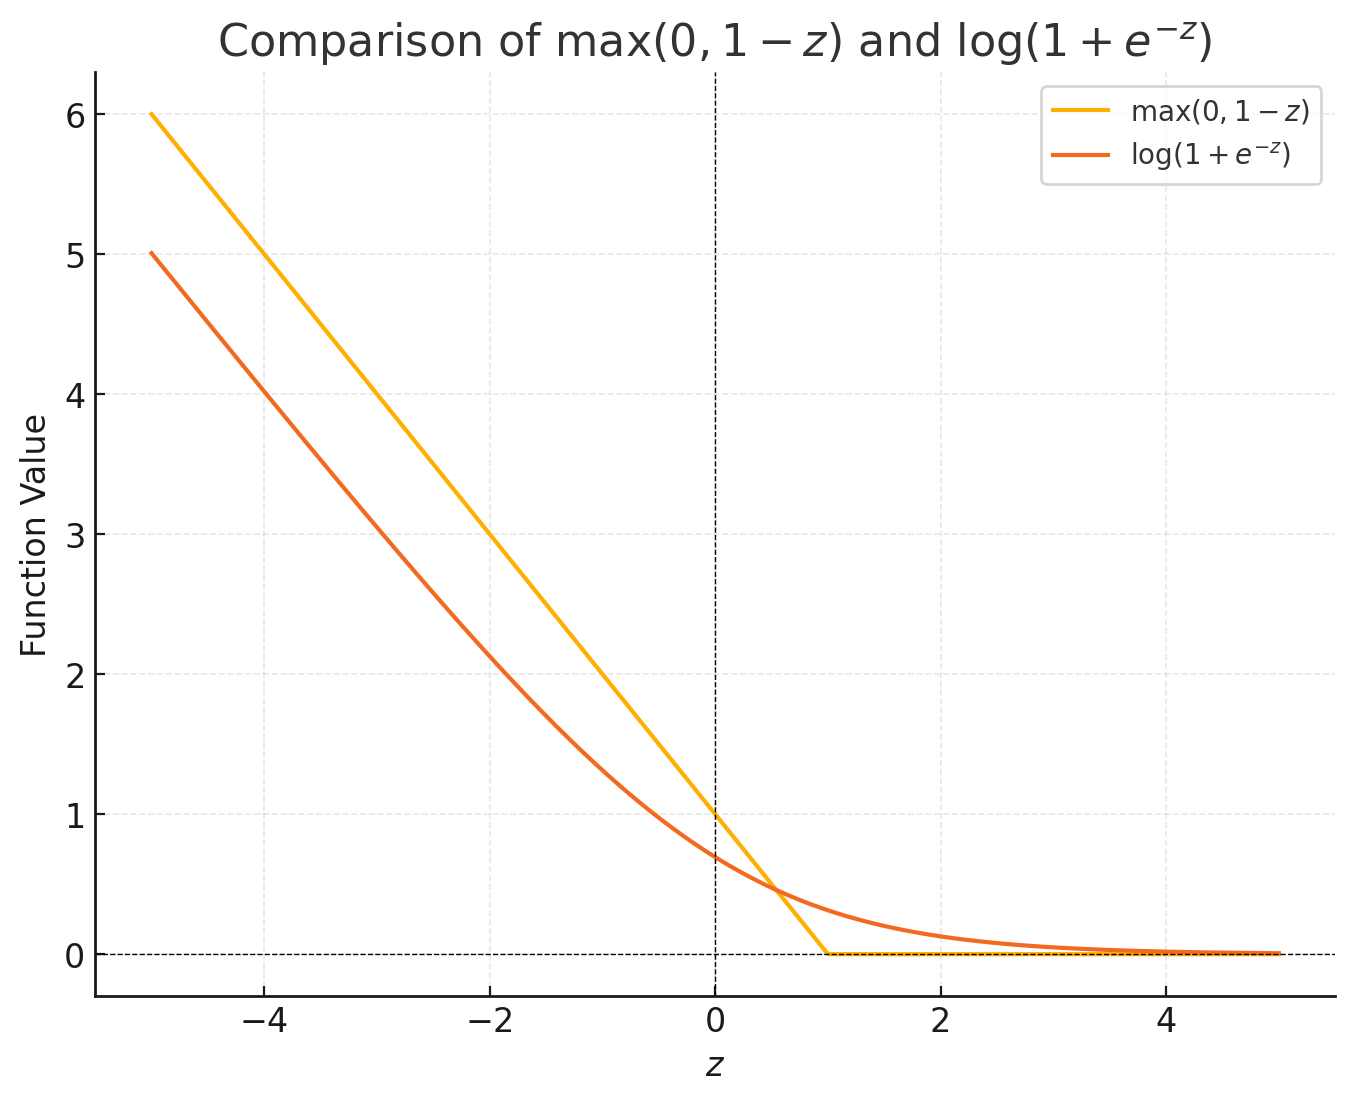
\includegraphics[width=0.75\textwidth]{.././assets/3.2.png}
    \end{figure}

    SVM and LR are both "linear" classifiers:

    \begin{itemize}
        \item Decision boundary $a^{\top} x+b=0$ is linear.
        \item Model completely ignores information perpendicular to $a$.
    \end{itemize}

    LR naturally generalizes to multi-class classification via softmax regression. Generalizing SVM to multi-class classification is trickier and less common.
\end{concept}

\begin{concept}[3.16][Maximum Likelihood Estimation $\cong$ minimizing KL divergence]
    Consider the setup where you have IID discrete random variables $X_{1}, \ldots, X_{N}$ that can take values $1, \ldots, k$. We model the probability masses with $\mathbb{P}_{\theta}(X=1), \ldots, \mathbb{P}_{\theta}(X=k)$. The \textbf{maximum likelihood estimation (MLE)} is obtained by solving

    $$
    \underset{\theta}{\operatorname{maximize}} \frac{1}{N} \sum_{i=1}^{N} \log \left(\mathbb{P}_{\theta}\left(X_{i}\right)\right)
    $$

    Next, define

    $$
    f_{\theta}=\left[\begin{array}{c}
    \mathbb{P}_{\theta}(X=1) \\
    \vdots \\
    \mathbb{P}_{\theta}(X=k)
    \end{array}\right], \quad \mathcal{P}\left(X_{1}, \ldots, X_{N}\right)=\frac{1}{N}\left[\begin{array}{c}
    \#\left(X_{i}=1\right) \\
    \vdots \\
    \#\left(X_{i}=k\right)
    \end{array}\right] .
    $$

    Then MLE is equivalent to minimizing the KL divergence from the model to the empirical distribution.

    $$
    \begin{gathered}
    \text{MLE} \\
    \mathbb{\Updownarrow} \\
    \underset{\theta}{\operatorname{minimize}} H \left( \mathcal{P}\left(X_{1}, \ldots, X_{N}\right), f_{\theta}\right) \\
    \mathbb{\Updownarrow} \\
    \underset{\theta}{\operatorname{minimize}} D_{\mathrm{KL}} \left( \mathcal{P}\left(X_{1}, \ldots, X_{N}\right), f_{\theta}\right) \\
    \end{gathered}
    $$

    One can also derive LR equivalently as the MLE.

    Generally, one can view the MLE as minimizing the KL divergence between the model and the empirical distribution. (For continuous random variables like the Gaussian, this requires extra work, since we haven't defined the KL divergence for continuous random variables.)

    In deep learning, the distance measure need not be KL divergence.
\end{concept}

\section{Prediction}

\begin{definition}[3.17][Estimation, Prediction]
    Finding $f \approx f_{\star}$ for unknown

    $$
    f_{\star}: \mathcal{X} \rightarrow \mathcal{P}(\mathcal{Y})
    $$

    is called \textbf{estimation}. When we consider a parameterized model $f_{\theta}$, finding $\theta$ is the estimation. However, estimation is usually not the end goal.

    The end goal is \textbf{prediction}. It is to use $f_{\theta} \approx f_{\star}$ on new data $X_{1}^{\prime}, \ldots, X_{M}^{\prime} \in \mathcal{X}$ to find labels $Y_{1}^{\prime}, \ldots, Y_{M}^{\prime} \in \mathcal{Y}$.
\end{definition}

\begin{concept}[3.18][Is prediction possible?]
    In the worst hypotheticals, prediction is impossible.

    \begin{itemize}
        \item Even though smoking is harmful for every other human being, how can we be 100% sure that this one person is not a mutant who benefits from the chemicals of a cigarette?
        \item Water freezes at $0^{\circ}$, but will the same be true tomorrow? How can we be 100% sure that the laws of physics will not suddenly change tomorrow?
    \end{itemize}

    Of course, prediction is possible in practice.

    Theoretically, prediction requires assumptions on the distribution of $X$ and the model of $f_{\star}$ is needed. This is in the realm of statistics of statistical learning theory.

    For now, we will take the view that if we predict known labels of the training data, we can reasonably hope to do well on the new data. (We will discuss the issue of generalization and overfitting later.)
\end{concept}

\begin{concept}[3.19][Training Data vs Test Data]
    When testing a machine learning model, it is \textbf{essential that one separates the training data with the test data}.

    In other classical disciplines using data, one performs a statistical hypothesis test to obtain a $p$-value. In ML, people do not do that.

    The only sure way to ensure that the model is doing well is to assess its performance on new data.

    Usually, training data and test data is collected together. This ensures that they have the same statistical properties. The assumption is that this test data will be representative of the actual data one intends to use machine learning on.
\end{concept}

\section{Datasets}

\begin{concept}[3.20][MNIST]
    Images of hand-written digits with $28 \times 28=784$ pixels and integervalued intensity between 0 and 255 . Every digit has a label in $\{0,1, \ldots, 8,9\}$.

    70,000 images (60,000 for training / 10,000 testing) of 10 almost balanced classes.

    One of the simplest data set used in machine learning.

    \begin{figure}[H]
        \centering
        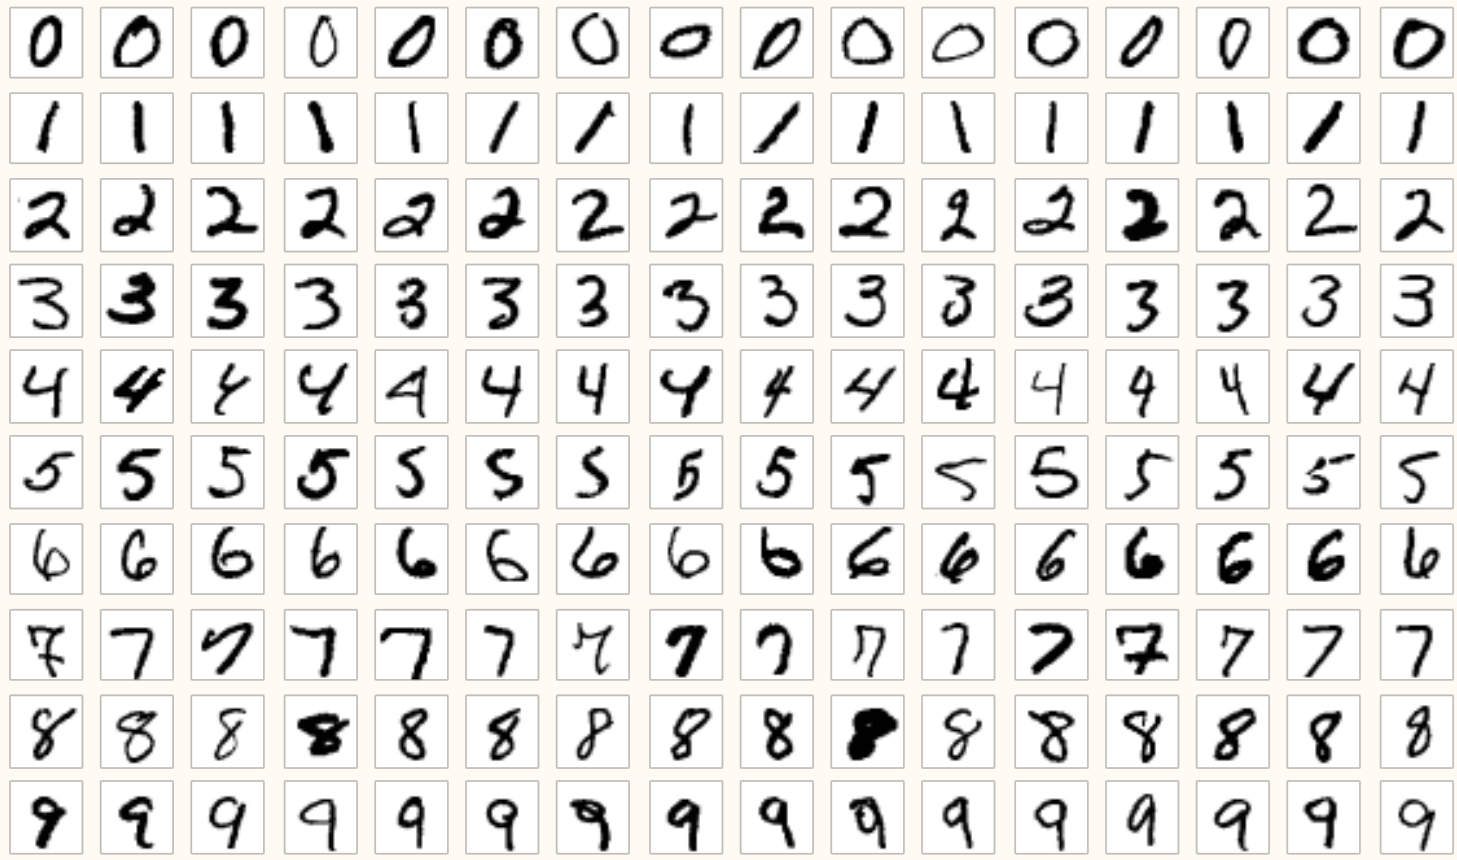
\includegraphics[width=0.75\textwidth]{.././assets/3.3.png}
    \end{figure}

    The USA government needed a standardized test to assess handwriting recognition software being sold to the government. So the NIST (National Institute of Standards and Technology) created the dataset in the 1990s. In 1990, NIST Special Database 1 distributed on CD-ROMs by mail. NIST SD 3 (1992) and SD 19 (1995) were improvements.

    Humans were instructed to fill out handwriting sample forms. However, humans cannot be trusted to follow instructions, so a lab technician performed "human ground truth adjudication".

    In 1998, Man LeCun, Corinna Cortes, Christopher J. C. Barges took the NIST dataset and modified it to create the MNIST dataset.
\end{concept}

\begin{concept}[3.21][CIFAR10]
    60,000 $32 \times 32$ color images in 10 (perfectly) balanced classes.

    \begin{figure}[H]
        \centering
        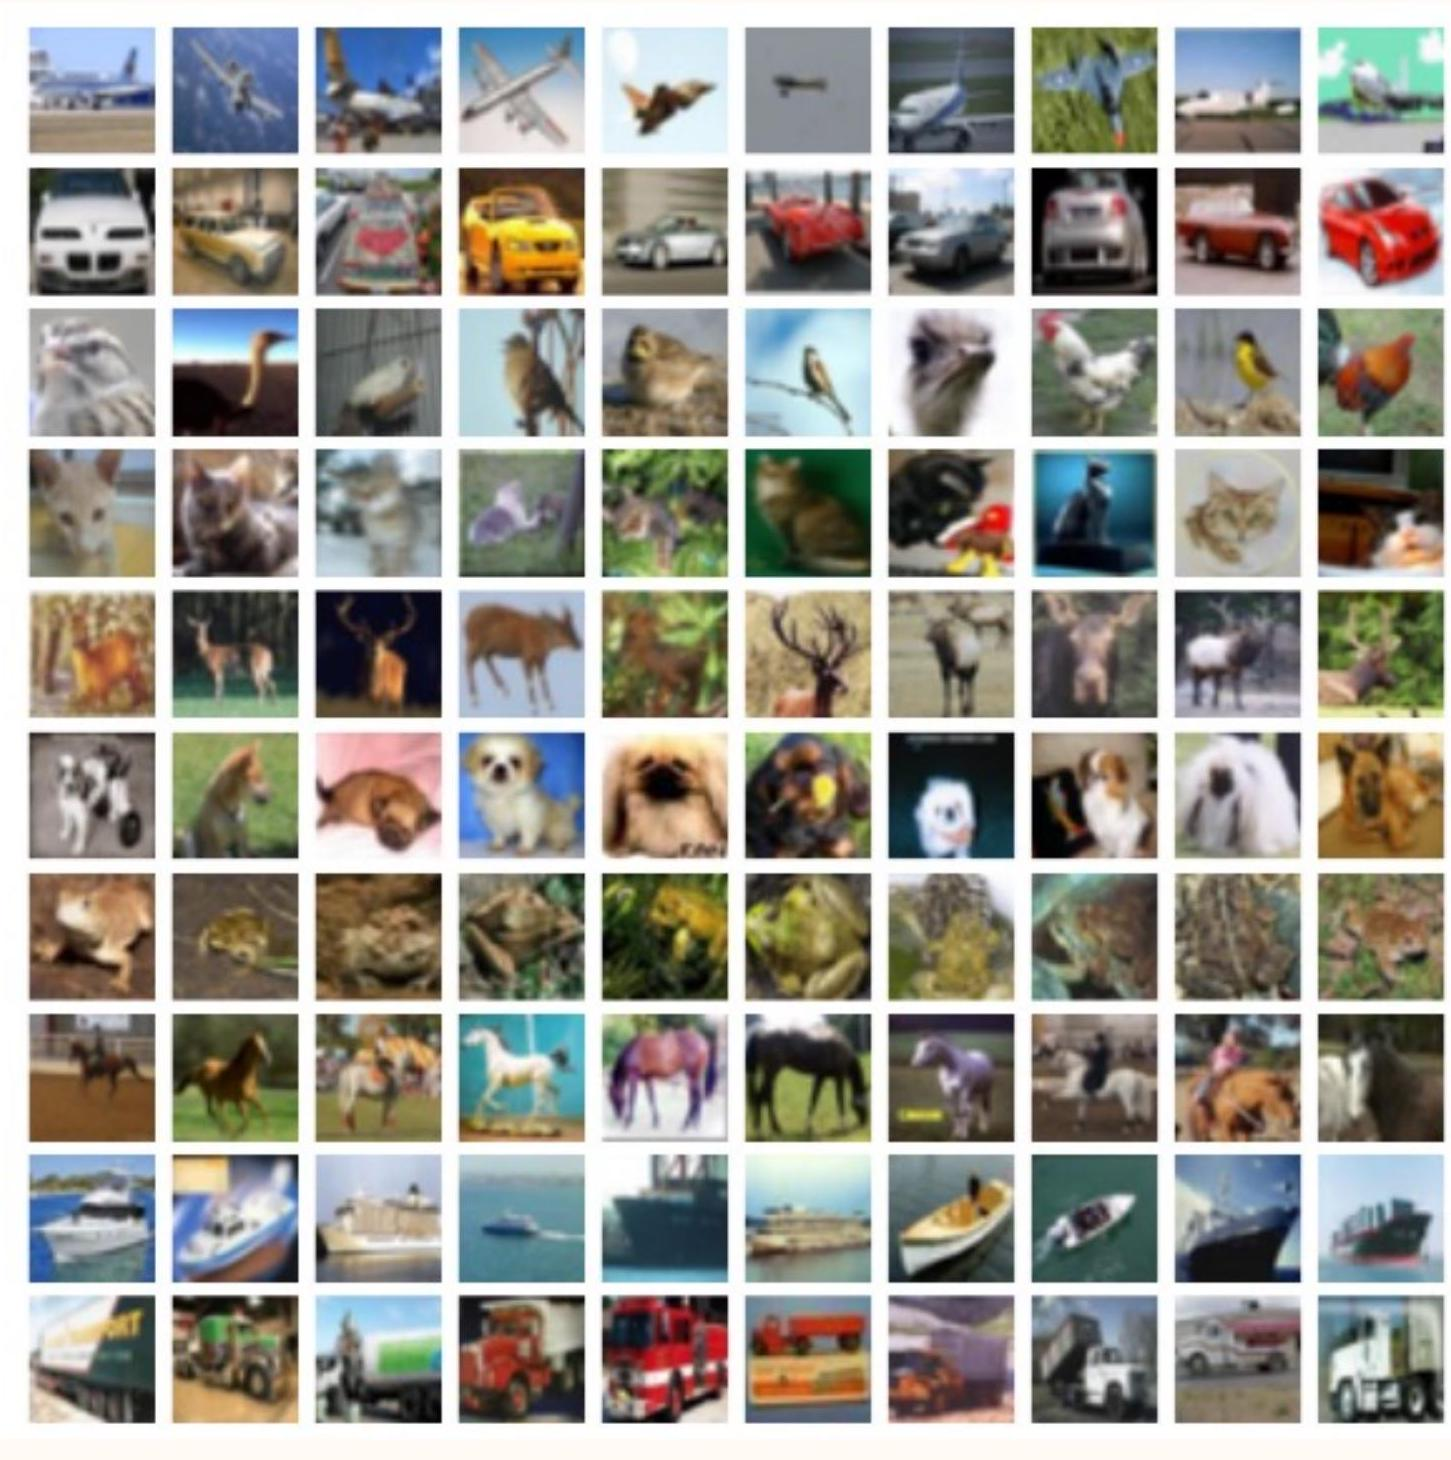
\includegraphics[width=0.75\textwidth]{.././assets/3.4.jpg}
    \end{figure}

    (There is no overlap between automobiles and trucks. “Automobile” includes sedans, SUVs, things of that sort. “Truck” includes only big trucks. Neither includes pickup trucks.)

    In 2008, a MIT and NYU team created the 80 million tiny images data set by searching on Google, Flickr, and Altavista for every non-abstract English noun and downscaled the images to $32 \times 32$. The search term provided an unreliable label for the image. This dataset was not very easy to use since the classes were too numerous.

    In 2009, Alex Krizhevsky published the CIFAR10, by distilling just a few classes and cleaning up the labels. Students were paid to verify the labels.

    The dataset was named CIFAR-10 after the funding agency Canadian Institute For Advanced Research.

    There is also a CIFAR-100 with 100 classes.
\end{concept}

\begin{concept}[3.22][Roles of Datasets in ML Research]
    An often underappreciated contribution.

    Good datasets play a crucial role in driving progress in ML research.

    Thinking about the dataset is the essential first step of understanding the feasibility of a ML task.

    Accounting for the cost of producing datasets and leveraging freely available data as much as possible (semi-supervised learning) is a recent trend in machine learning.
\end{concept}

\chapter{Deep Neural Networks}

\section{Deep Neural Networks}

\begin{concept}[4.1][LR can be seen as 1-layer (shallow) neural network.]
    In LR, we solve

    $$
    \underset{a \in \mathbb{R}^{p}, b \in \mathbb{R}}{\operatorname{minimize}} \frac{1}{N} \sum_{i=1}^{N} \ell\left(f_{\theta}\left(X_{i}\right), Y_{i}\right)
    $$

    where $\ell\left(y_{1}, y_{2}\right)=\log \left(1+e^{-y_{1} y_{2}}\right)$ and $f_{\theta}$ is linear.

    We can view $f_{\theta}(x)=O=a^{\top} x+b$ as a 1-layer (shallow) neural network.

    \begin{figure}[H]
        \centering
        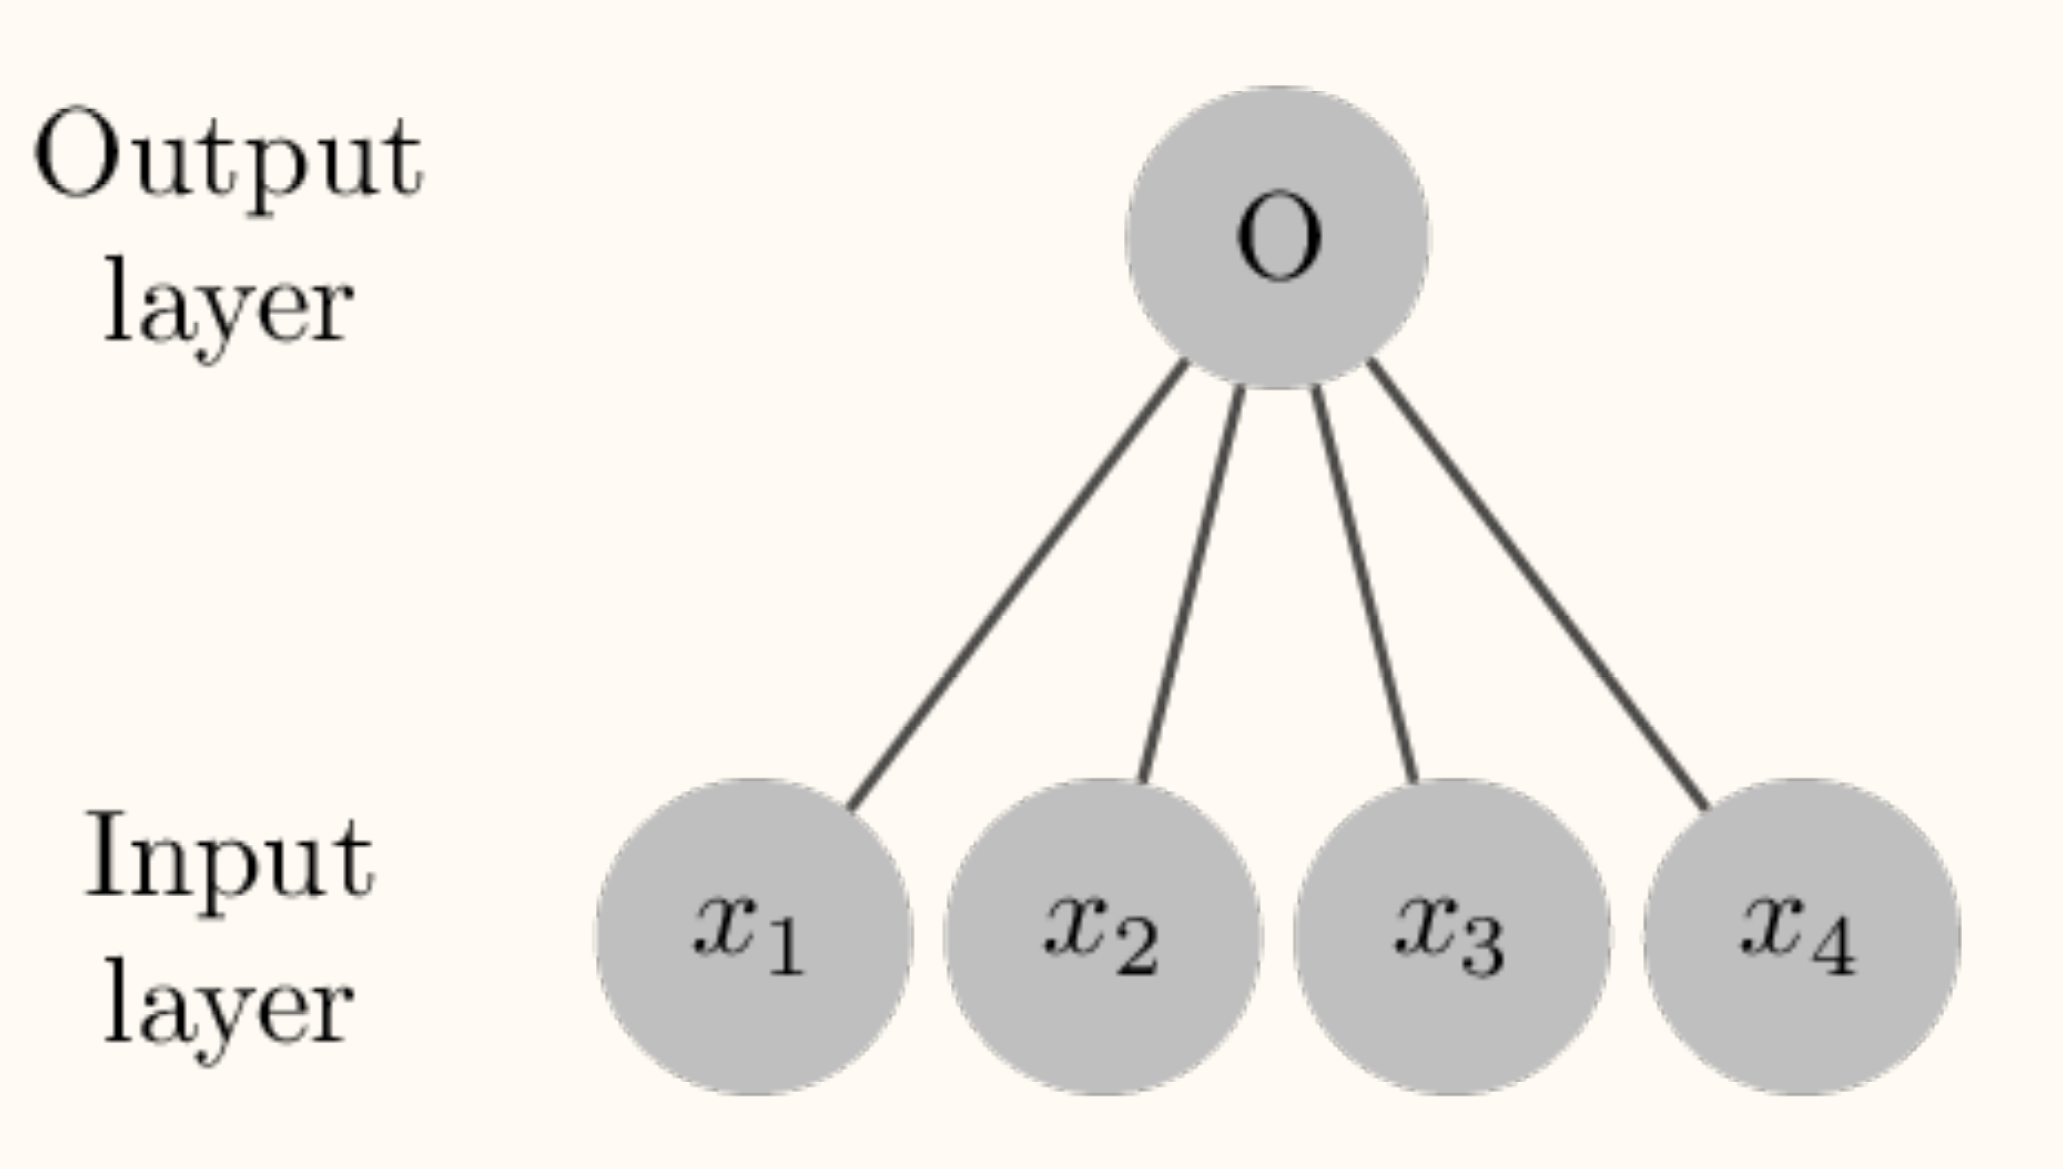
\includegraphics[width=0.5\textwidth]{.././assets/4.1.png}
    \end{figure}
\end{concept}

\begin{concept}[4.2][Deep Neural Networks with Nonlinearities]
    What happens if we stack multiple linear layers?

    \textbf{Problem}: This is pointless because composition of linear functions is linear.\\
    ( $O = W_2 h = W_2(W_1 x) = (W_2 W_1) x \leftarrow$ linear in $x$ )

    \textbf{Solution}: use a nonlinear activation function $\sigma$ to inject nonlinearities.

    \begin{figure}[H]
        \centering
        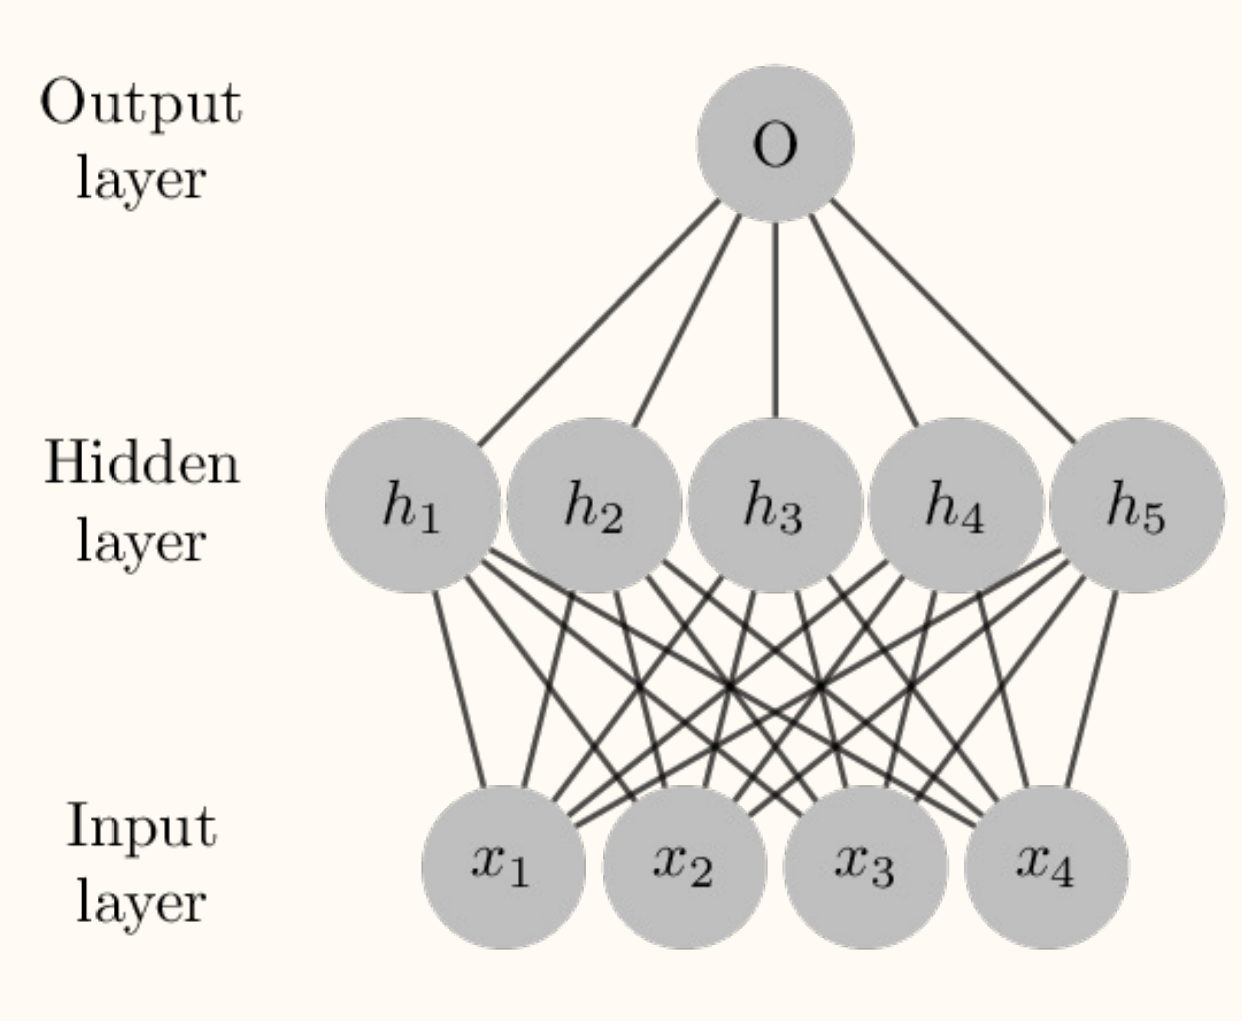
\includegraphics[width=0.5\textwidth]{.././assets/4.2.png}
    \end{figure}

    Hidden layer $h=\sigma(W_1 x)$ ($\sigma$ : Nonlinear function)\\
    Output layer $O=W_2 h = W_2 \sigma(W_1 x) \leftarrow$ nonlinear in $x$
\end{concept}

\begin{definition}[4.3][Common Activation Functions]
    \begin{itemize}
        \item
        \textbf{Rectified Linear Unit (ReLU)}

        $$
        \operatorname{ReLU}(z)=\max (z, 0)
        $$

        \begin{figure}[H]
            \centering
            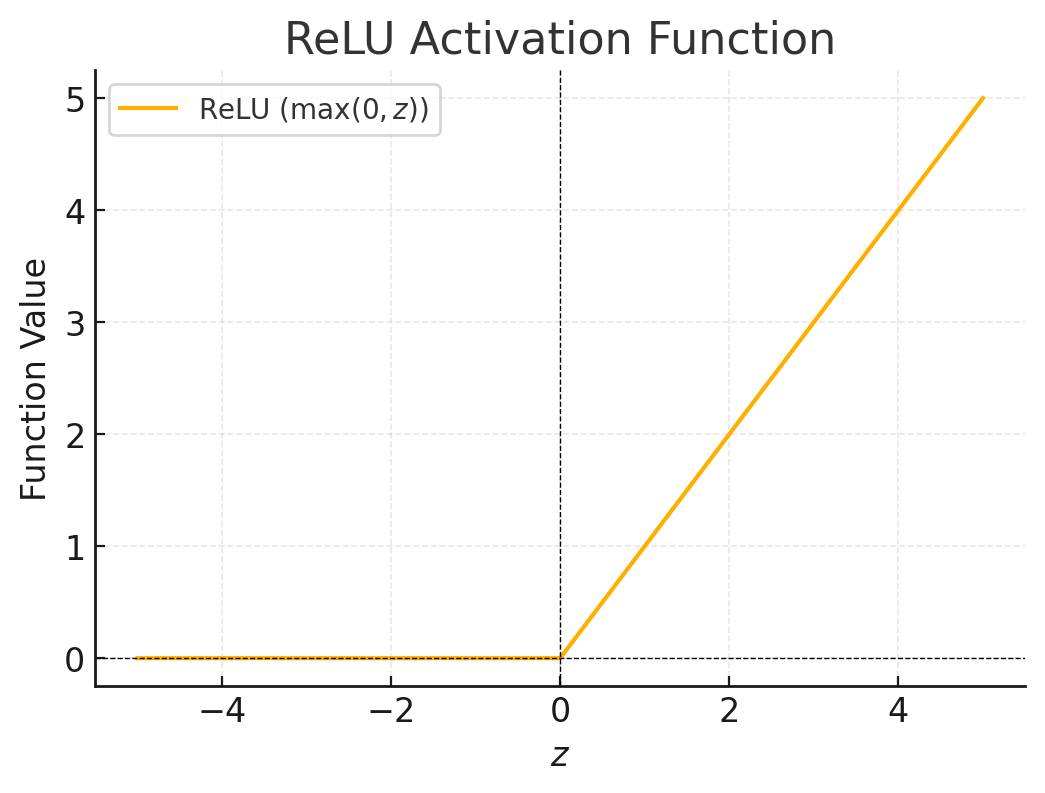
\includegraphics[width=0.5\textwidth]{.././assets/4.3.png}
        \end{figure}
        \item
        \textbf{Sigmoid}

        $$
        \operatorname{Sigmoid}(z)=\frac{1}{1+e^{-z}}
        $$

        \begin{figure}[H]
            \centering
            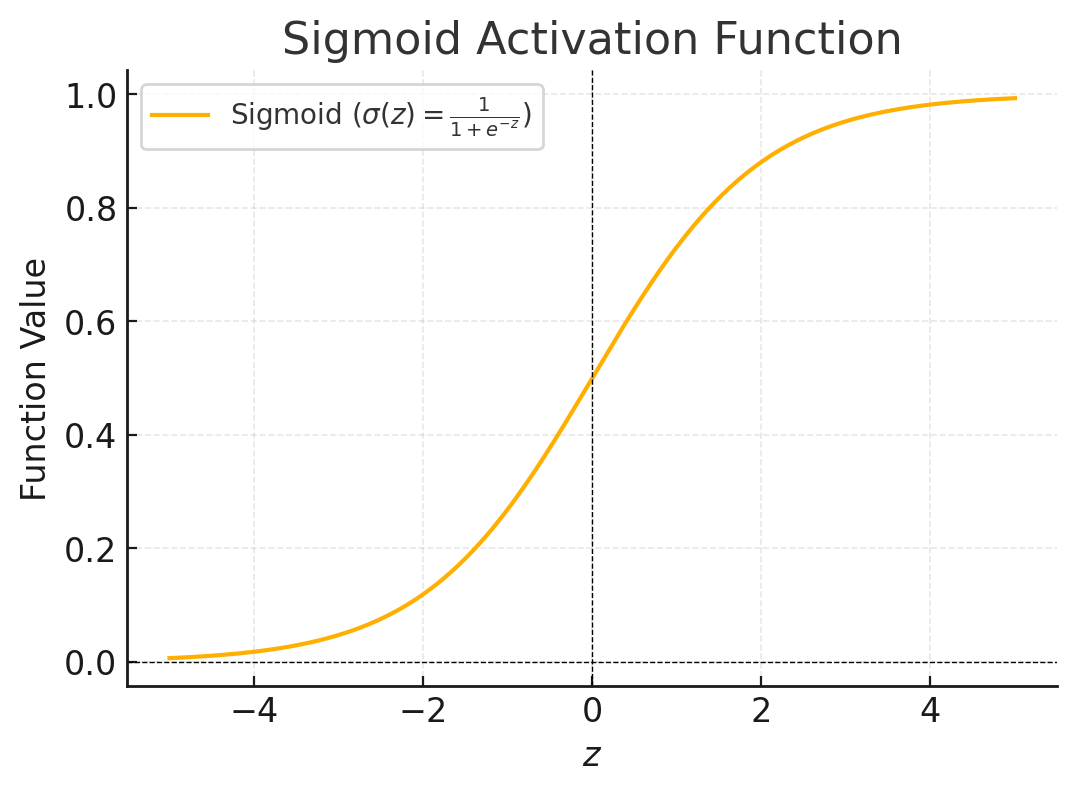
\includegraphics[width=0.5\textwidth]{.././assets/4.4.png}
        \end{figure}
        \item
        \textbf{Hyperbolic Tangent}

        $$
        \tanh (z)=\frac{1-e^{-2 z}}{1+e^{-2 z}}
        $$

        \begin{figure}[H]
            \centering
            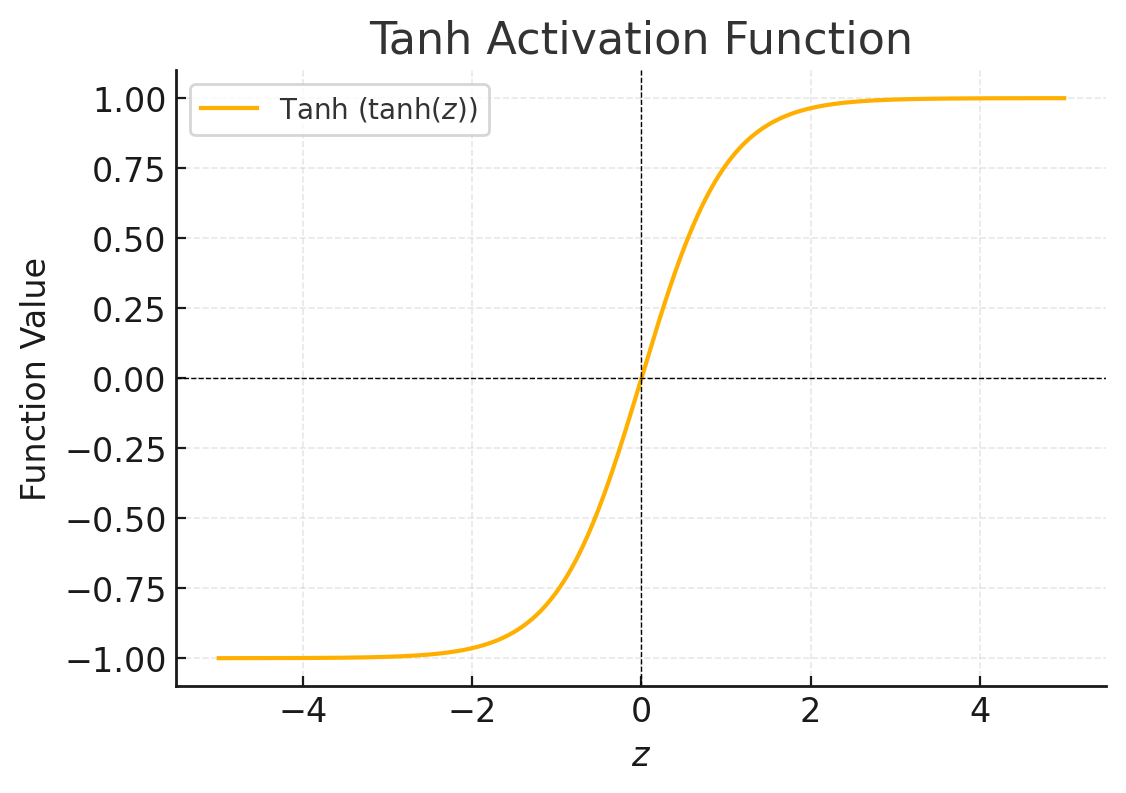
\includegraphics[width=0.5\textwidth]{.././assets/4.5.png}
        \end{figure}
    \end{itemize}
\end{definition}

\begin{definition}[4.4][Multilayer Perceptron (MLP)]
    The \textbf{multilayer perceptron}, also called \textbf{fully connected neural network}, has the form

    $$
    \begin{aligned}
    y_{L}= & W_{L} y_{L-1}+b_{L} \\
    y_{L-1}= & \sigma\left(W_{L-1} y_{L-2}+b_{L-1}\right) \\
    & \vdots \\
    y_{2}= & \sigma\left(W_{2} y_{1}+b_{2}\right) \\
    y_{1}= & \sigma\left(W_{1} x+b_{1}\right),
    \end{aligned}
    $$

    where $x \in \mathbb{R}^{n_{0}}, W_{\ell} \in \mathbb{R}^{n_{\ell} \times n_{\ell-1}}, b_{\ell} \in \mathbb{R}^{n_{\ell}}$, and $n_{L}=1$. To clarify, $\sigma$ is applied element-wise.
\end{definition}

\begin{definition}[4.5][Linear Layer (with Batches)]
    \begin{itemize}
        \item Input tensor: $X \in \mathbb{R}^{B \times n}, B$ batch size, $n$ number of indices.
        \item Output tensor: $Y \in \mathbb{R}^{B \times m}, B$ batch size, $m$ number of indices.
    \end{itemize}

    With weight $A \in \mathbb{R}^{m \times n}$, bias $b \in \mathbb{R}^{m}, k=1, \ldots B$, and $i=1, \ldots, m$ :

    $$
    Y_{k, i}=\sum_{j=1}^{n} A_{i, j} X_{k, j}+b_{i}
    $$

    Operation is independent across elements of the batch.

    If \verb|bias=False|, then $b=0$.
\end{definition}

\section{Multi-Class Classification}

\begin{definition}[4.6][Multi-Class Classification Problem]
    Consider supervised learning with data $X_{1}, \ldots, X_{N} \in \mathbb{R}^{n}$ and labels $Y_{1}, \ldots, Y_{N} \in\{1, \ldots, k\}$. (A $k$ class classification problem.) Assume there exists a function $f_{\star}: \mathbb{R}^{n} \rightarrow \Delta^{k}$ mapping from data to label probabilities. Here, $\Delta^{k} \subset \mathbb{R}^{k}$ denotes the set of probability mass functions on $\{1, \ldots, k\}$.

    Define the empirical distribution $\mathcal{P}(y) \in \mathbb{R}^{k}$ as the one-hot vector:

    $$
    (\mathcal{P}(y))_{i}=\left\{\begin{array}{cc}
    1 & \text { if } y=i \\
    0 & \text { otherwise }
    \end{array}\right.
    $$

    for $i=1, \ldots, k$.
\end{definition}

\begin{definition}[4.7][Softmax Function]
    \textbf{Softmax} function $\mu: \mathbb{R}^{k} \rightarrow \Delta^{k}$ is defined by

    $$
    \mu_{i}(z)=(\mu(z))_{i}=\frac{e^{z_{i}}}{\sum_{j=1}^{k} e^{z_{j}}}
    $$

    for $i=1, \ldots, k$, where $z=\left(z_{1}, \ldots, z_{k}\right) \in \mathbb{R}^{k}$. Since

    $$
    \sum_{i=1}^{k} \mu_{i}(z)=1, \quad \mu>0
    $$

    Name "softmax" is a misnomer. "Softargmax" would be more accurate

    \begin{itemize}
        \item $\mu(z) \not \approx \max (z)$
        \item $\mu(z) \approx \operatorname{argmax}(z)$
    \end{itemize}

    Examples:

    $$
    \mu\left(\left[\begin{array}{l}
    1 \\
    2 \\
    3
    \end{array}\right]\right)=\left[\begin{array}{l}
    0.09 \\
    0.24 \\
    0.6
    \end{array}\right],
    \mu\left(\left[\begin{array}{c}
    999 \\
    0 \\
    -2
    \end{array}\right]\right) \approx\left[\begin{array}{l}
    1 \\
    0 \\
    0
    \end{array}\right],
    \mu\left(\left[\begin{array}{c}
    -2 \\
    -2 \\
    -99
    \end{array}\right]\right) \approx\left[\begin{array}{c}
    0.5 \\
    0.5 \\
    0
    \end{array}\right]
    $$
\end{definition}

\begin{definition}[4.8][Softmax Regression (SR)]
    In \textbf{softmax regression (SR)}:

    Choose the model

    $$
    \mu\left(f_{A, b}(x)\right)=\frac{1}{\sum_{i=1}^{k} e^{a_{i}^{\top} x+b_{i}}}\left[\begin{array}{c}
    e^{a_{1}^{\top} x+b_{1}} \\
    e^{a_{2}^{\top} x+b_{2}} \\
    \vdots \\
    e^{a_{k}^{\top} x+b_{k}}
    \end{array}\right], \quad f_{A, b}(x)=A x+b, A=\left[\begin{array}{c}
    a_{1}^{\top} \\
    a_{2}^{\top} \\
    \vdots \\
    a_{k}^{\top}
    \end{array}\right] \in \mathbb{R}^{k \times n}, \quad b=\left[\begin{array}{c}
    b_{1} \\
    b_{2} \\
    \vdots \\
    b_{k}
    \end{array}\right] \in \mathbb{R}^{k} .
    $$

    Minimize KL-Divergence (or cross entropy) from the model $\mu\left(f_{A, b}\left(X_{i}\right)\right)$ output probabilities to the empirical distribution $\mathcal{P}\left(Y_{i}\right)$.

    $$
    \underset{A \in \mathbb{R}^{k \times n}, b \in \mathbb{R}^{k}}{\operatorname{minimize}} \sum_{i=1}^{N} D_{\mathrm{KL}}\left(\mathcal{P}\left(Y_{i}\right) \| \mu\left(f_{A, b}\left(X_{i}\right)\right)\right) \Longleftrightarrow \underset{A \in \mathbb{R}^{k \times n}, b \in \mathbb{R}^{k}}{\operatorname{minimize}} \sum_{i=1}^{N} H\left(\mathcal{P}\left(Y_{i}\right), \mu\left(f_{A, b}\left(X_{i}\right)\right)\right)
    $$
\end{definition}

\begin{concept}[4.9][Other Expression of Softmax Regression]
    $$
    \begin{gathered}
    \underset{A \in \mathbb{R}^{k \times n}, b \in \mathbb{R}^{k}}{\operatorname{minimize}} \sum_{i=1}^{N} H\left(\mathcal{P}\left(Y_{i}\right), \mu\left(f_{A, b}\left(X_{i}\right)\right)\right) \\
    \mathbb{\Updownarrow} \\
    \underset{A \in \mathbb{R}^{k \times n}, b \in \mathbb{R}^{k}}{\operatorname{minimize}} \frac{1}{N} \sum_{i=1}^{N}-\log \left(\mu_{Y_{i}}\left(f_{A, b}\left(X_{i}\right)\right)\right) \\
    \mathbb{\Updownarrow} \\
    \underset{A \in \mathbb{R}^{k \times n}, b \in \mathbb{R}^{k}}{\operatorname{minimize}} \frac{1}{N} \sum_{i=1}^{N}-\log \left(\frac{\exp \left(a_{Y_{i}}^{\top} X_{i}+b_{Y_{i}}\right)}{\sum_{j=1}^{k} \exp \left(a_{j}^{\top} X_{i}+b_{j}\right)}\right) \\
    \mathbb{\Updownarrow} \\
    \underset{A \in \mathbb{R}^{k \times n}, b \in \mathbb{R}^{k}}{\operatorname{minimize}} \frac{1}{N} \sum_{i=1}^{N}\left(-\left(a_{Y_{i}}^{\top} X_{i}+b_{Y_{i}}\right)+\log \left(\sum_{j=1}^{k} \exp \left(a_{j}^{\top} X_{i}+b_{j}\right)\right)\right)
    \end{gathered}
    $$
\end{concept}

\begin{definition}[4.10][Cross Entropy Loss]
    Where $f \in \mathbb{R}^{k}, y \in \{1, 2, \cdots, k\}$, the \textbf{cross entropy loss} is

    $$
    \ell^{\mathrm{CE}}(f, y)=-\log \left(\frac{\exp \left(f_{y}\right)}{\sum_{j=1}^{k} \exp \left(f_{j}\right)}\right)
    $$
\end{definition}

\begin{concept}[4.11][SR uses cross entropy loss as loss function.]
    $$
    \begin{gathered}
    \underset{A \in \mathbb{R}^{k \times n}, b \in \mathbb{R}^{k}}{\operatorname{minimize}} \sum_{i=1}^{N} H\left(\mathcal{P}\left(Y_{i}\right), \mu\left(f_{A, b}\left(X_{i}\right)\right)\right) \\
    \mathbb{\Updownarrow} \\
    \underset{A \in \mathbb{R}^{k \times n}, b \in \mathbb{R}^{k}}{\operatorname{minimize}} \frac{1}{N} \sum_{i=1}^{N}-\log \left(\frac{\exp \left(a_{Y_{i}}^{\top} X_{i}+b_{Y_{i}}\right)}{\sum_{j=1}^{k} \exp \left(a_{j}^{\top} X_{i}+b_{j}\right)}\right) \\
    \mathbb{\Updownarrow} \\
    \underset{A \in \mathbb{R}^{k \times n}, b \in \mathbb{R}^{k}}{\operatorname{minimize}} \frac{1}{N} \sum_{i=1}^{N} \ell^{\mathrm{CE}}\left(f_{A, b}\left(X_{i}\right), Y_{i}\right)
    \end{gathered}
    $$

    \begin{itemize}
        \item SR = linear model $f_{A, b}$ with cross entropy loss:
    \end{itemize}

    $$
    \underset{A \in \mathbb{R}^{k \times n}, b \in \mathbb{R}^{k}}{\operatorname{minimize}} \frac{1}{N} \sum_{i=1}^{N} \ell^{\mathrm{CE}}\left(f_{A, b}\left(X_{i}\right), Y_{i}\right) \Longleftrightarrow \underset{A \in \mathbb{R}^{k \times n}, b \in \mathbb{R}^{k}}{\operatorname{minimize}} \sum_{i=1}^{N} D_{\mathrm{KL}}\left(\mathcal{P}\left(Y_{i}\right) \| \mu\left(f_{A, b}\left(X_{i}\right)\right)\right)
    $$

    \begin{itemize}
        \item
        The natural extension of SR is to consider

        $$
        \underset{\theta \in \mathbb{R}^{p}}{\operatorname{minimize}} \frac{1}{N} \sum_{i=1}^{N} \ell^{\mathrm{CE}}\left(f_{\theta}\left(X_{i}\right), Y_{i}\right) \Leftrightarrow \underset{\theta \in \mathbb{R}^{p}}{\operatorname{minimize}} \quad \sum_{i=1}^{N} D_{\mathrm{KL}}\left(\mathcal{P}\left(Y_{i}\right) \| \mu\left(f_{\theta}\left(X_{i}\right)\right)\right)
        $$

        where $f_{\theta}$ is a deep neural network.
    \end{itemize}
\end{concept}

\section{GPUs in Deep Learning}

\begin{concept}[4.12][History of GPU Computing]
    Rendering graphics involves computing many small tasks in parallel. Graphics cards provide many small processors to render graphics.

    In 1999, Nvidia released GeForce 256 and introduced programmability in the form of vertex and pixel shaders. Marketed as the first \textbf{'Graphical Processing Unit (GPU)'}.

    Researchers quickly learned how to implement linear algebra by mapping matrix data into textures and applying shaders.

    In 2007, Nvidia released \textbf{'Compute Unified Device Architecture (CUDA)'}, which enabled general purpose computing on a CUDA-enabled GPUs.

    Unlike CPUs which provide fast serial processing, GPUs provide massive parallel computing with its numerous slower processors.

    The 2008 financial crisis hit Nvidia very hard as GPUs were luxury items used for games. This encouraged Nvidia to invest further in \textbf{'General Purpose GPUs (GPGPU)'} and create a more stable consumer base.
\end{concept}

\begin{concept}[4.13][CPU Computing Model]
    \begin{figure}[H]
        \centering
        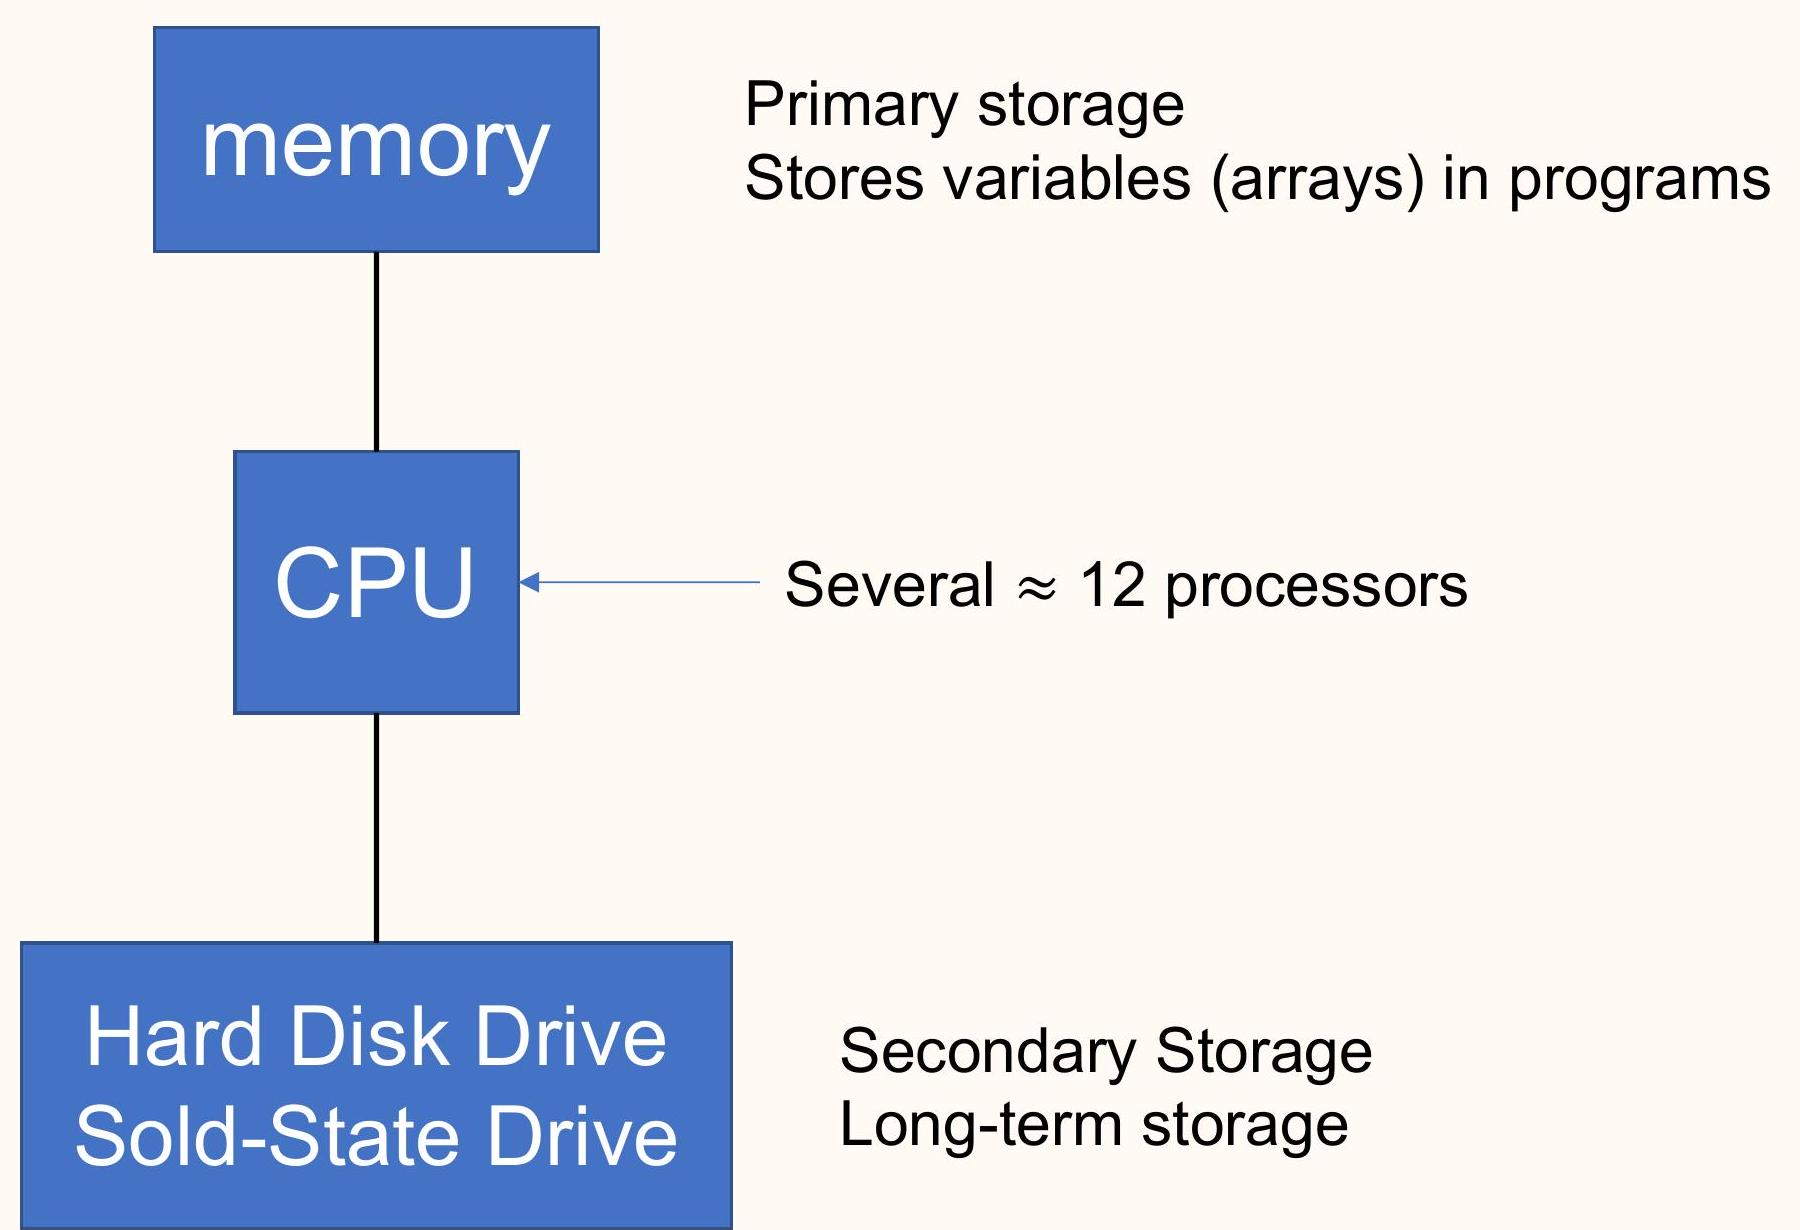
\includegraphics[width=0.75\textwidth]{.././assets/4.6.jpg}
    \end{figure}
\end{concept}

\begin{concept}[4.14][GPU Computing Model]
    \begin{figure}[H]
        \centering
        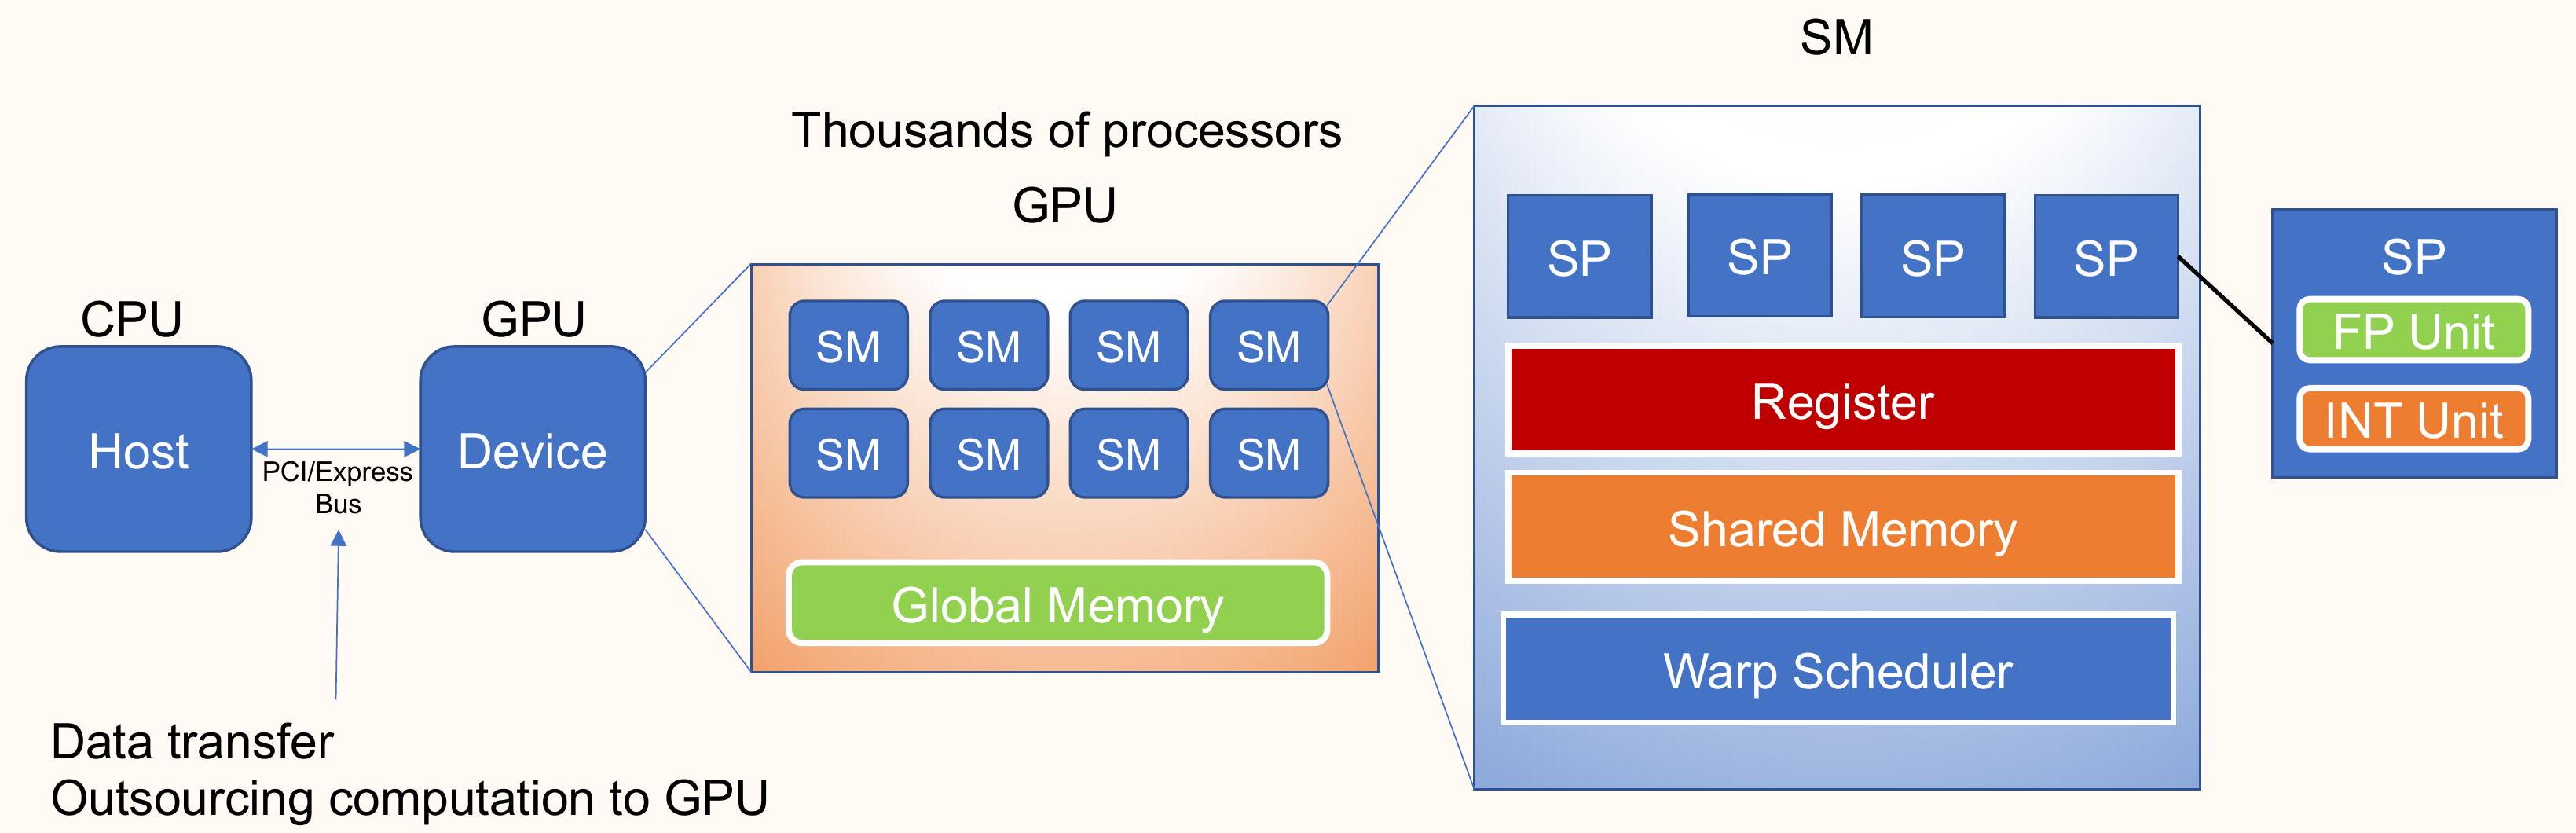
\includegraphics[width=1.0\textwidth]{.././assets/4.7.jpg}
    \end{figure}
\end{concept}

\begin{concept}[4.15][GPUs for Machine Learning]
    Raina et al.'s 2009* paper demonstrated that GPUs can be used to train large neural networks. (This was not the first to use of GPUs in machine learning, but it was one of the most influential.)

    Modern deep learning is driven by big data and big compute, respectively provided by the internet and GPUs.

    Krizhevsky et al.'s 2012 landmark paper introduced AlexNet trained on GPUs and kickstarted the modern deep learning boom.

    (R. Raina, A. Madhavan, and A. Y. Ng , Large-scale Deep Unsupervised Learning using Graphics Processors, ICML, 2009. / 
    A. Krizhevsky, I. Sutskever, G. E. Hinton, ImageNet Classification with Deep Convolutional Neural Networks, NeurIPS, 2012.)
\end{concept}

\begin{concept}[4.16][Deep Learning on GPUs]
    Steps for training neural network on GPU:

    \begin{enumerate}
        \item
        Create the neural network on CPU and send it to GPU. Neural network parameters stay on GPU.

        \begin{itemize}
            \item Sometimes you load parameters from CPU to GPU.
        \end{itemize}
        \item
        Select data batch (image, label) and send it to GPU every iteration

        \begin{itemize}
            \item Data for real-world setups is large, so keeping all data on GPU is infeasible.
        \end{itemize}
        \item On GPU, compute network output (forward pass)
        \item On GPU, compute gradients (backward pass)
        \item On GPU, perform gradient update
        \item
        Once trained, perform prediction on GPU.

        \begin{itemize}
            \item Send test data to GPU.
            \item Compute network output.
            \item Retrieve output on CPU.
            \item Alternatively, neural network can be loaded on CPU and prediction can be done on CPU.
        \end{itemize}
    \end{enumerate}
\end{concept}

\chapter*{Chapter 2 Code}

\href{https://drive.google.com/file/d/15kXC3cJUV63gZNfXK6JdPPuSrwQZBzI8/view?usp=sharing}{Chapter 2 Code}

\part{Convolutional Neural Networks}

\chapter{Convolutional Neural Networks}

\section{Convolutional Layers}

\begin{concept}[5.1][Pros and Cons of Fully Connected Layers]
    Advantages of fully connected layers:

    \begin{itemize}
        \item Simple.
        \item Very general, in theory. (Sufficiently large MLPs can learn any function, in theory.)
    \end{itemize}

    Disadvantage of fully connected layers:

    \begin{itemize}
        \item Too many trainable parameters.
        \item Does not encode shift equivariance/invariance and therefore has poor inductive bias. (More on this later.)
    \end{itemize}
\end{concept}

\begin{concept}[5.2][Shift Equivarience/Invariance in Vision]
    Many tasks in vision are equivariant/invariant with respect shifts/translations.

    \begin{figure}[H]
        \centering
        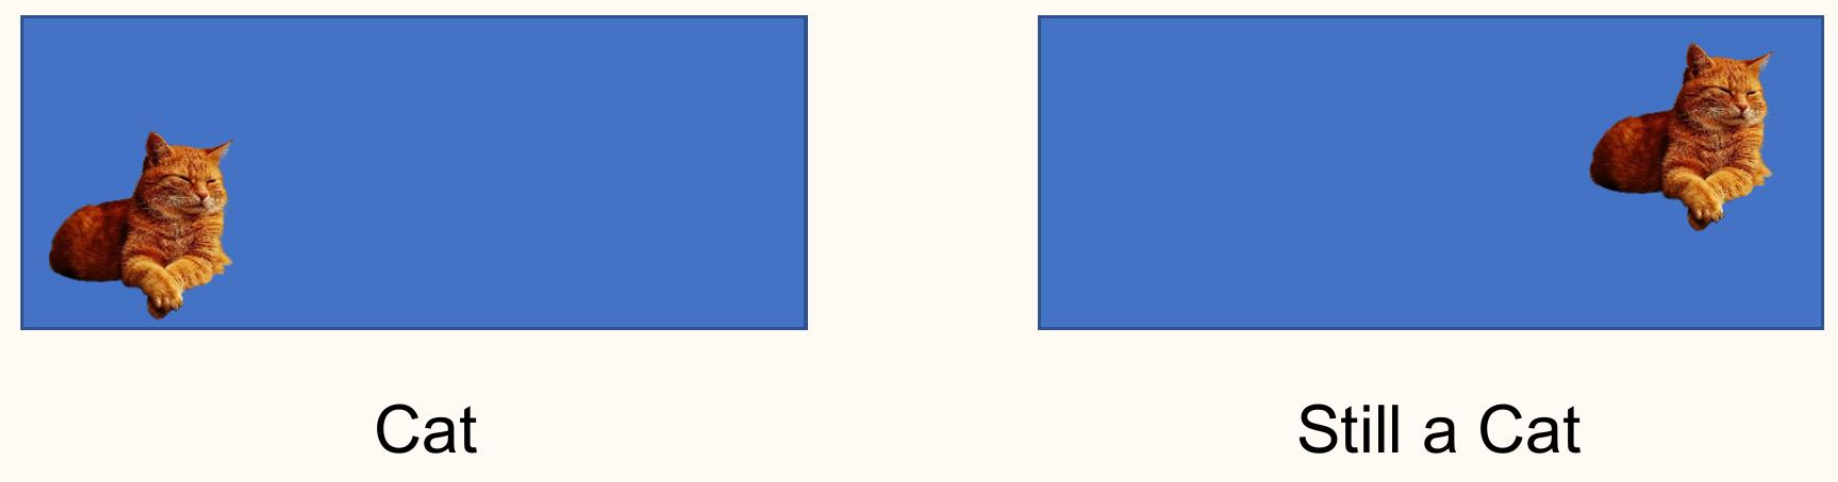
\includegraphics[width=0.75\textwidth]{.././assets/5.1.png}
    \end{figure}

    Roughly speaking, equivariance/invariance means shifting the object does not change the meaning (it only changes the position).

    Logistic regression (with a single fully connected layer) does not encode shift invariance.

    Since convolution is equivariant with respect to translations, constructing neural network layers with them is a natural choice.
\end{concept}

\begin{definition}[5.3][2D Convolutional Layer]
    \begin{itemize}
        \item $B$ : batch size
        \item $C_{\text{in}}$ : \# of input channels
        \item $C_{\text{out}}$ : \# of output channels
        \item $m, n$ : \# of vertical and horizontal indices of input
        \item $f_1, f_2$ : \# of vertical and horizontal indices of filter
    \end{itemize}

    \par\noindent\textcolor{gray}{\hdashrule{\textwidth}{0.4pt}{1pt 2pt}}

    \begin{itemize}
        \item Input tensor : $X \in \mathbb{R}^{B \times C_{\text {in }} \times m \times n}$
        \item Output tensor : $Y \in \mathbb{R}^{B \times C_{\text {out }} \times\left(m-f_{1}+1\right) \times\left(n-f_{2}+1\right)}$
        \item Filter : $w \in \mathbb{R}^{C_{\text {out }} \times C_{\text {in }} \times f_{1} \times f_{2}}$
        \item Bias : $b \in \mathbb{R}^{C_{\text{out}}}$
    \end{itemize}

    \par\noindent\textcolor{gray}{\hdashrule{\textwidth}{0.4pt}{1pt 2pt}}

    For $k = 1, \dots, B, \quad \ell = 1, \dots, C_{\text{out}}, \quad i = 1, \dots, m-f_1+1, \quad j = 1, \dots, n-f_2+1$:

    $$
    Y_{k, \ell, i, j}=\sum_{\gamma=1}^{c_{\text {in }}} \sum_{\alpha=1}^{f_{1}} \sum_{\beta=1}^{f_{2}} w_{\ell, \gamma, \alpha, \beta} X_{k, \gamma, i+\alpha-1, j+\beta-1}+b_{\ell}
    $$

    Operation is independent across elements of the batch.
    The vertical and horizontal indices are referred to as spatial dimensions.
    If \verb|bias=False|, then $b=0$.

    \par\noindent\textcolor{gray}{\hdashrule{\textwidth}{0.4pt}{1pt 2pt}}

    Convolve a filter with an image : slide the filter spatially over the image and compute dot products.

    Take a $C_{\text {in }} \times f_{1} \times f_{2}$ chunk of the image and take the inner product with $w$ and add bias $b$.
\end{definition}

\begin{example}[5.4][Example of 2D Convolutional Layer]
    \begin{figure}[H]
        \centering
        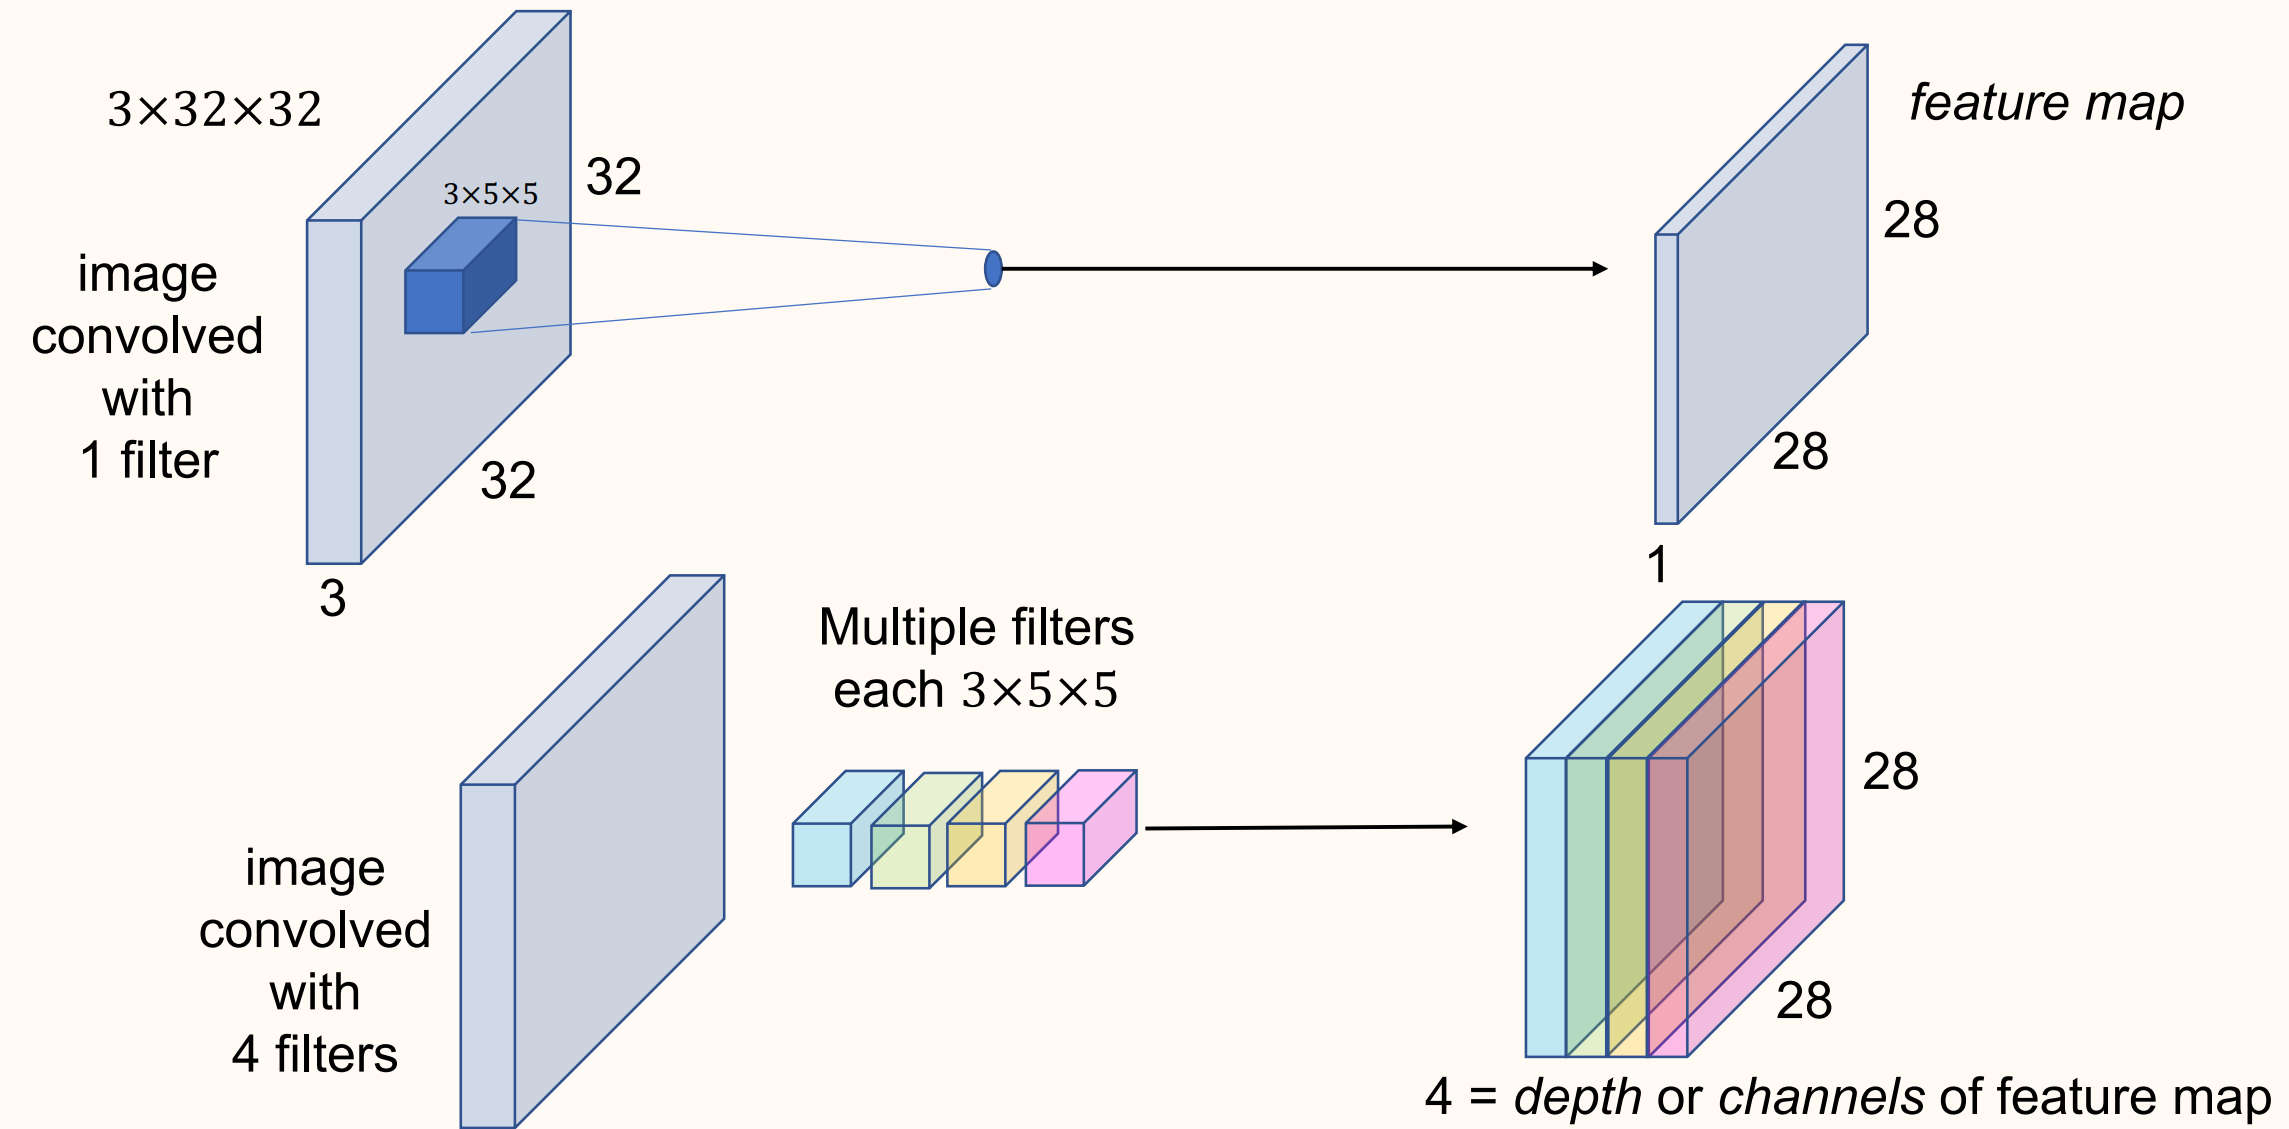
\includegraphics[width=1.0\textwidth]{.././assets/5.2.png}
    \end{figure}

    \begin{itemize}
        \item $B = 1, C_{\text{in}} = 3, C_{\text{out}} = 4, m=n=32, f_1=f_2=5$
        \item Input tensor : $X \in \mathbb{R}^{1 \times 3 \times 32 \times 32}$
        \item Output tensor : $Y \in \mathbb{R}^{1 \times 4 \times 28 \times 28}$
        \item Filter : $w \in \mathbb{R}^{4 \times 3 \times 5 \times 5}$
        \item Bias : $b \in \mathbb{R}^{4}$
    \end{itemize}
\end{example}

\begin{concept}[5.5][Zero Padding]
    \begin{itemize}
        \item \textbf{Problem}
    \end{itemize}

    Spatial dimension is reduced when passed through convolutional layers.

    \begin{figure}[H]
        \centering
        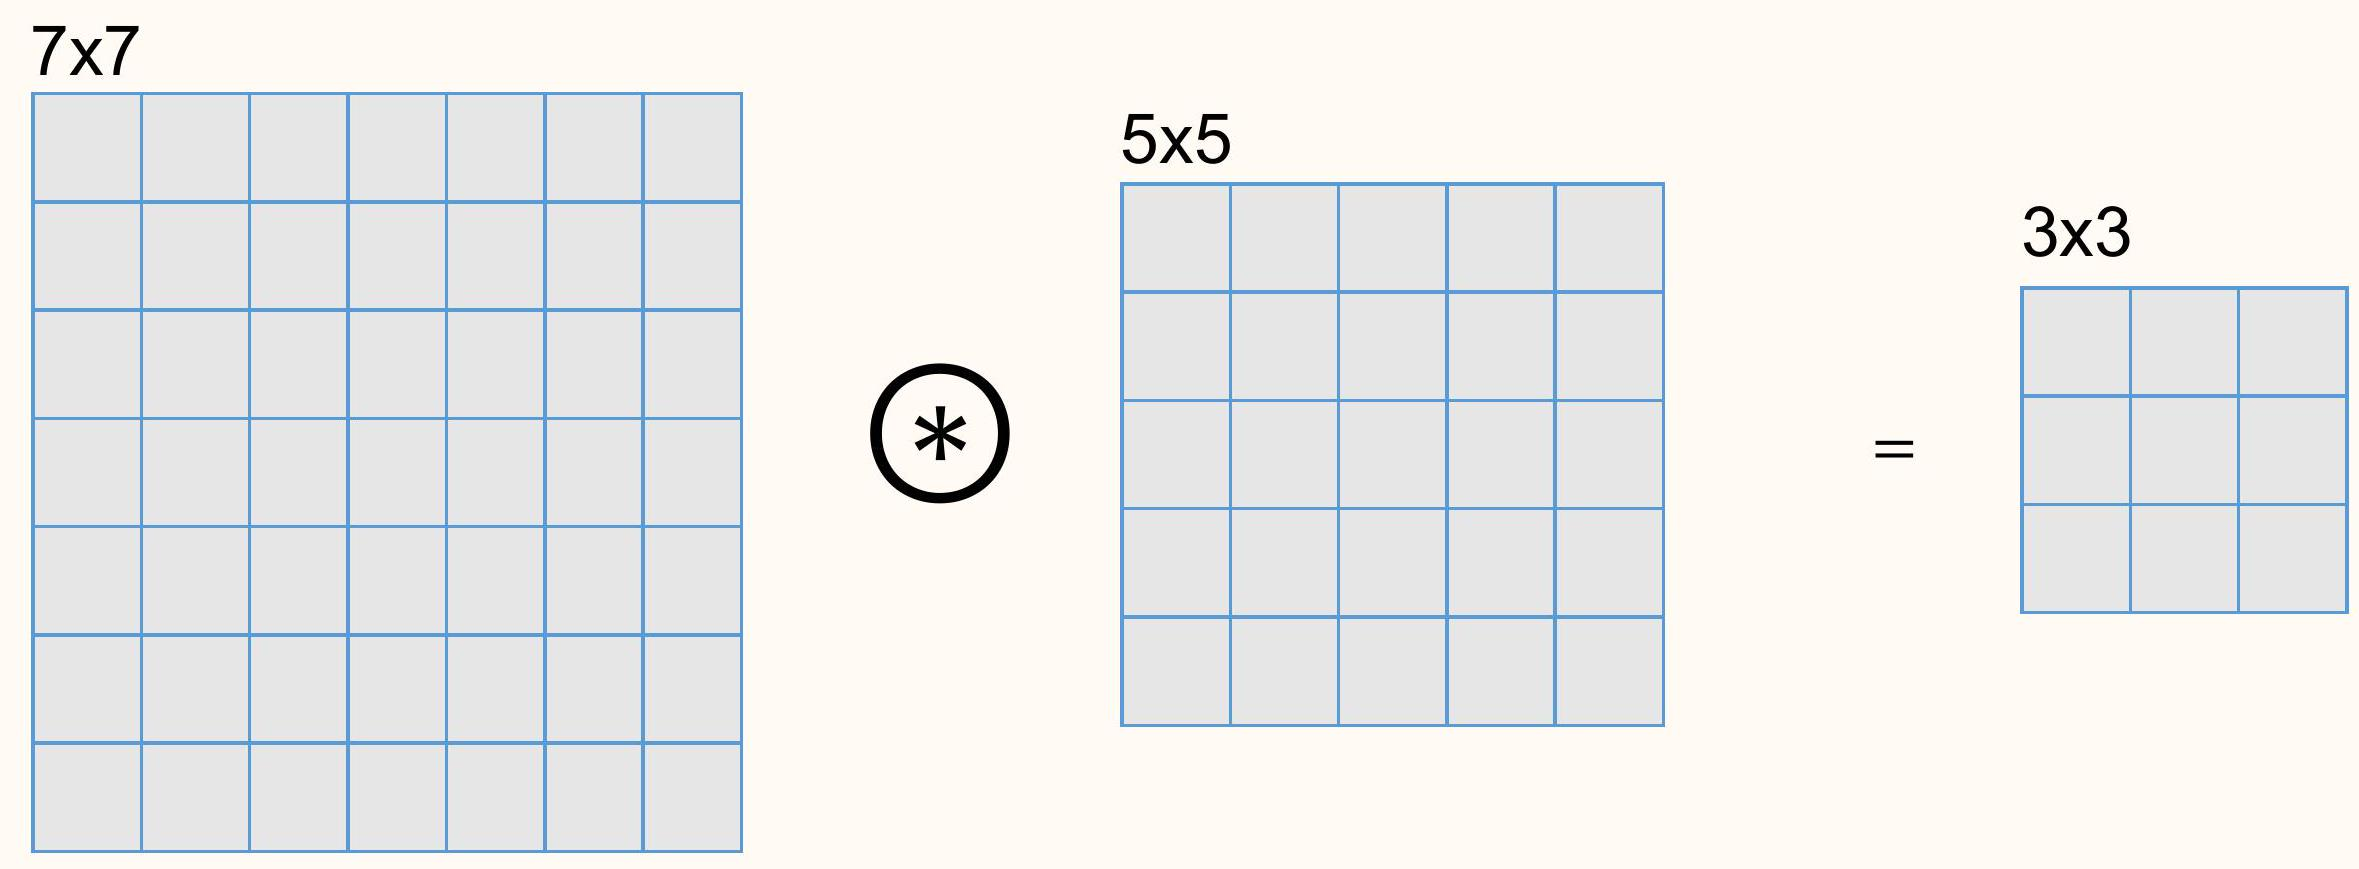
\includegraphics[width=1.0\textwidth]{.././assets/5.3.jpg}
    \end{figure}

    $(C \times 7 \times 7$ image$) \circledast(C \times 5 \times 5$ filter$)=(1 \times 3 \times 3$ feature map$)$.
    Spatial dimension 7 reduced to 3.

    \par\noindent\textcolor{gray}{\hdashrule{\textwidth}{0.4pt}{1pt 2pt}}

    \begin{itemize}
        \item \textbf{Solution}
    \end{itemize}

    \textbf{Zero padding} on boundaries can preserve spatial dimension through convolutional layers.

    \begin{figure}[H]
        \centering
        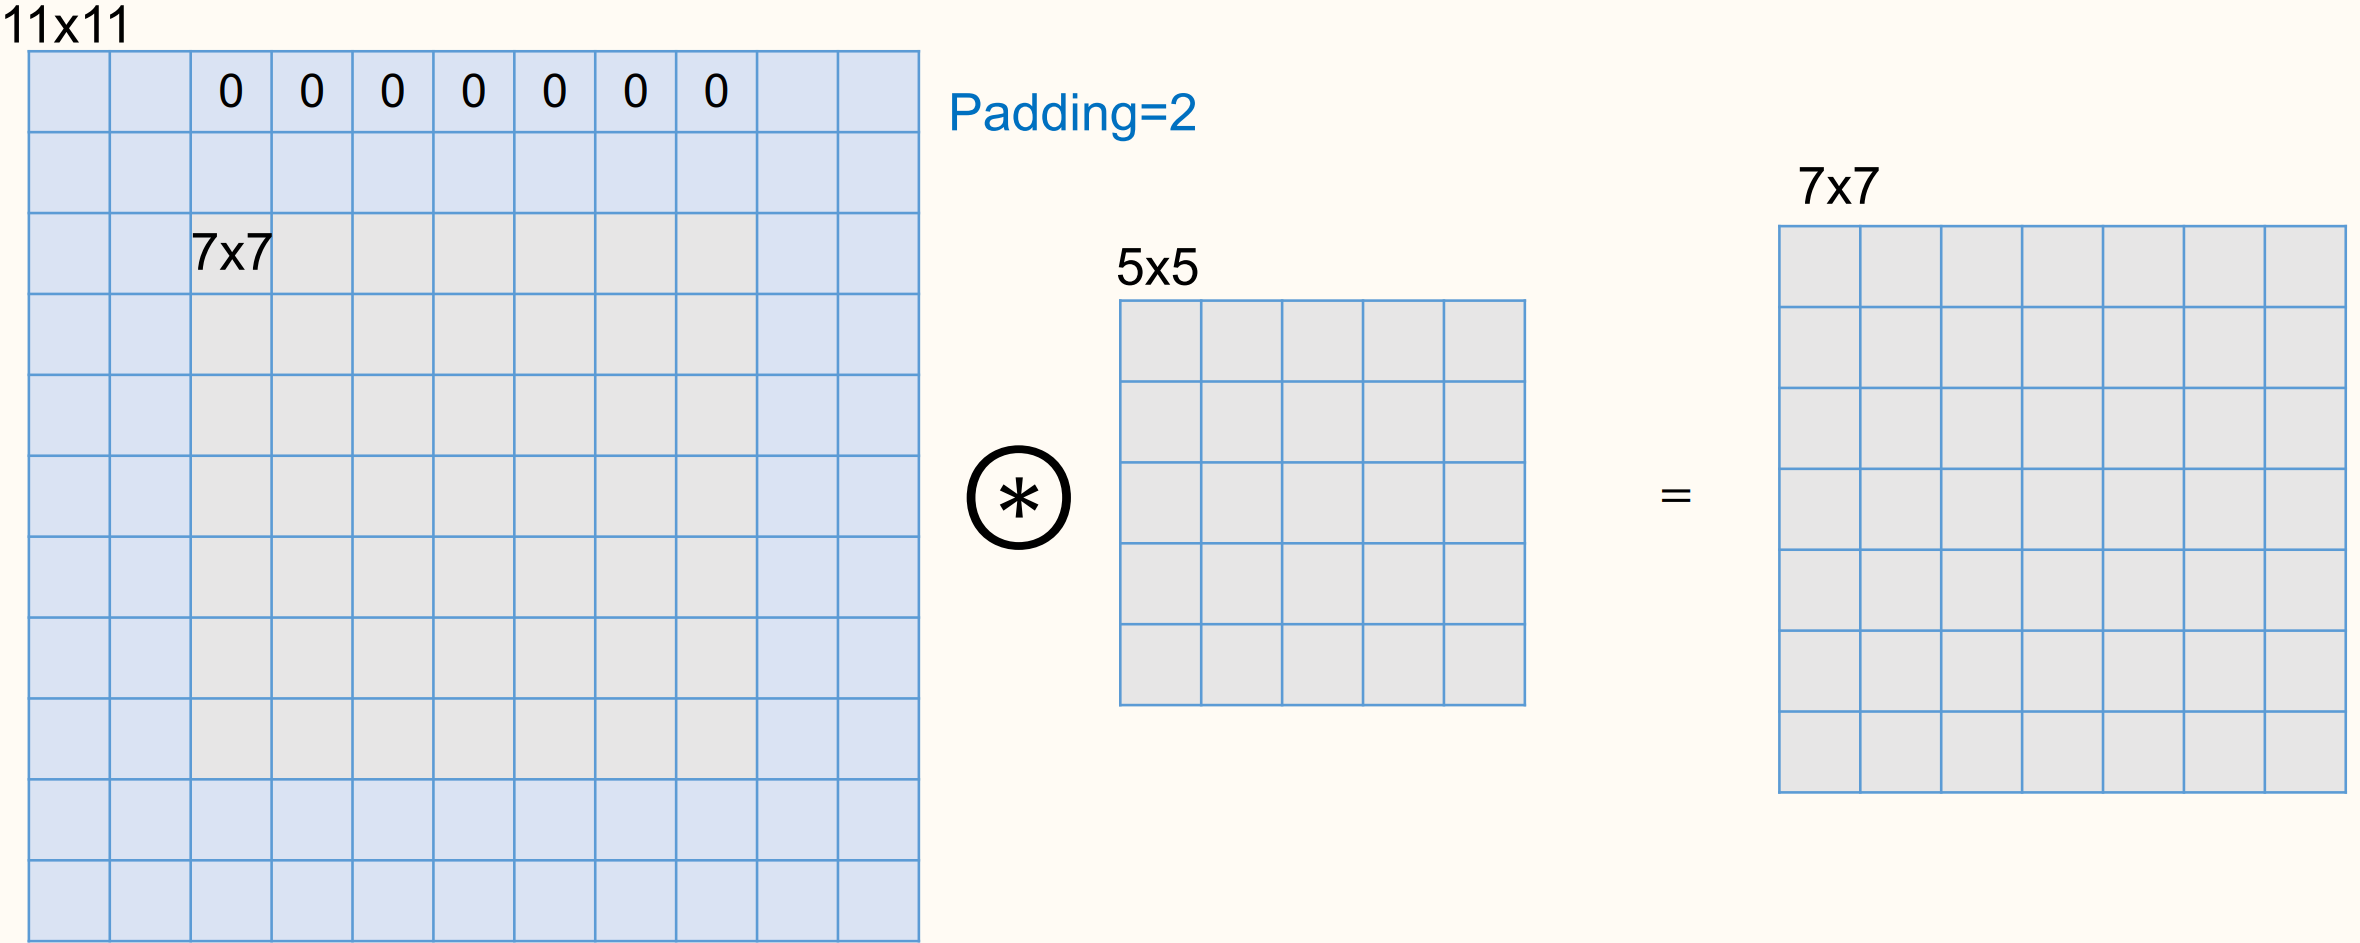
\includegraphics[width=1.0\textwidth]{.././assets/5.4.png}
    \end{figure}

    $(C \times 7 \times 7$ image with zero padding $=2) \circledast(C \times 5 \times 5$ filter$)=(1 \times 7 \times 7$ feature map$)$.
    Spatial dimension is preserved.
\end{concept}

\begin{concept}[5.6][Stride]
    The horizontal/vertical distance of two adjacent inner product calculations with the filter when sliding it across the image is called \textbf{stride}.
    It is originally set to 1, but can be adjusted.

    \begin{itemize}
        \item $(7 \times 7$ image$) \circledast(3 \times 3$ filter$)$ with stride $1=($output $5 \times 5)$
        \item
        $(7 \times 7$ image$) \circledast(3 \times 3$ filter$)$ with stride $2=($output $3 \times 3)$

        \begin{figure}[H]
            \centering
            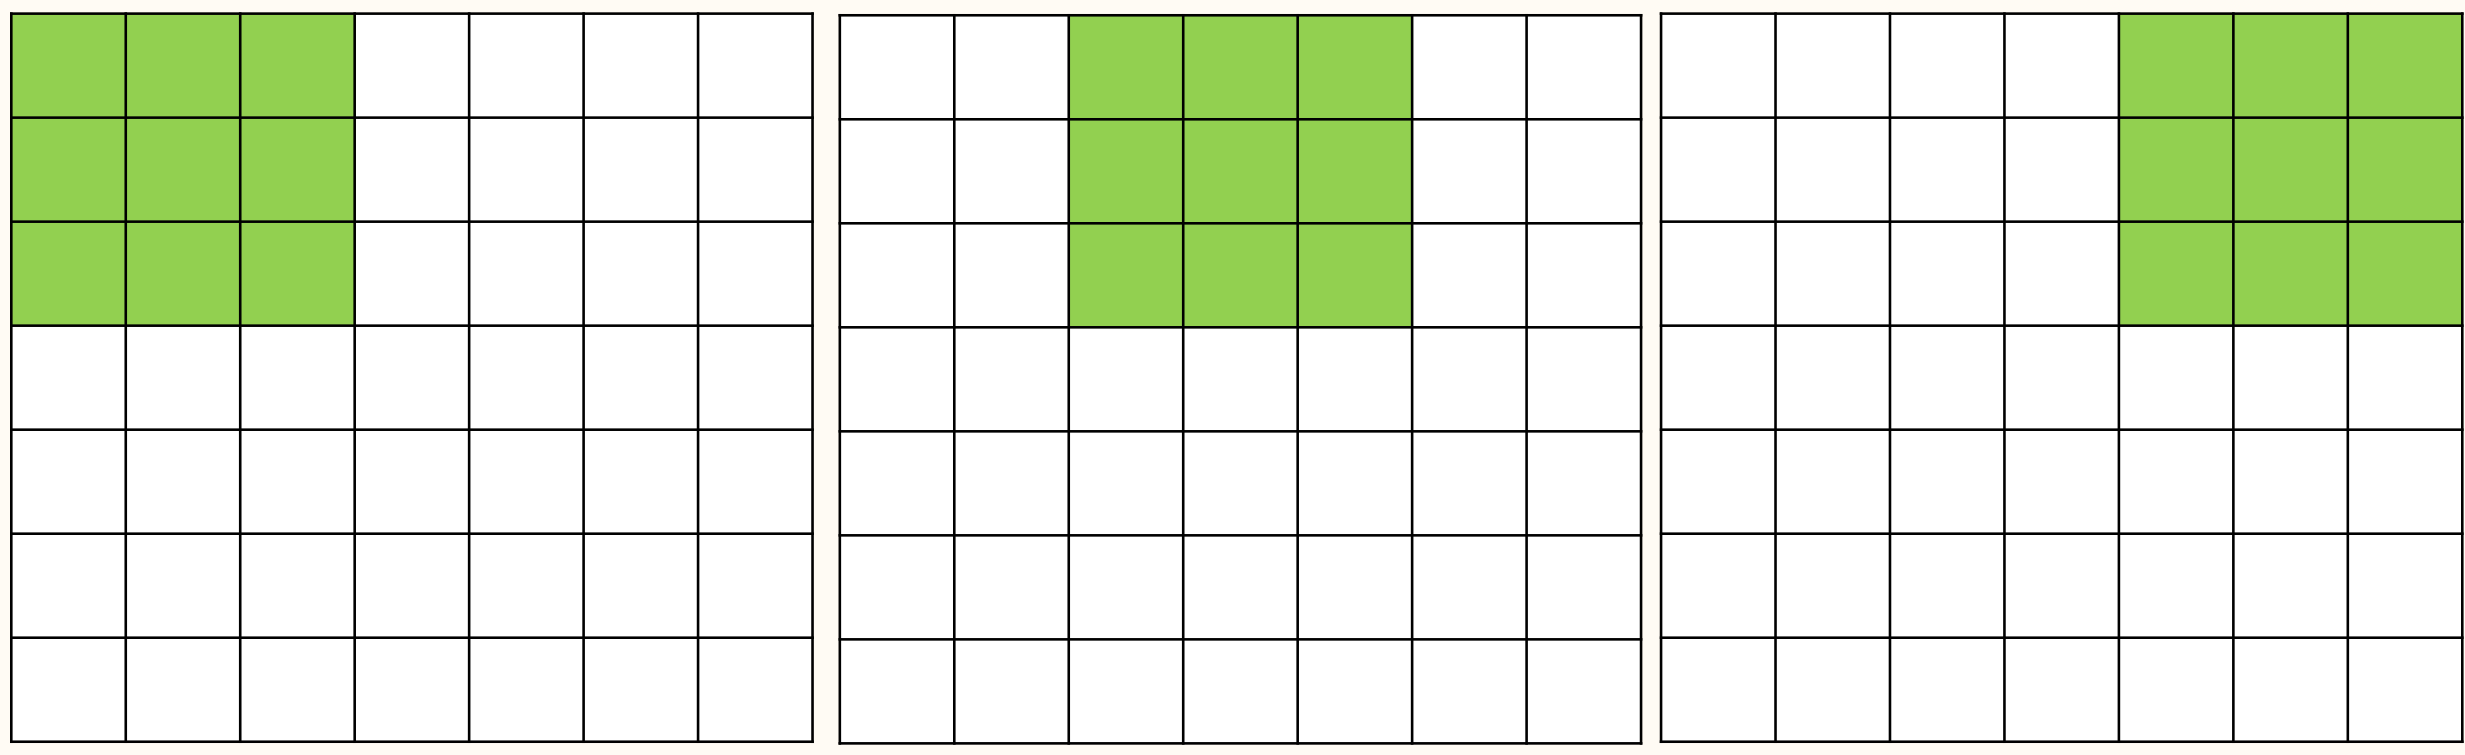
\includegraphics[width=1.0\textwidth]{.././assets/5.5.png}
        \end{figure}
        \item $(7 \times 7$ image with zero padding $=1) \circledast(3 \times 3$ filter$)$ with stride $3=($output $3 \times 3)$
    \end{itemize}
\end{concept}

\begin{concept}[5.7][Convolution Summary]
    \begin{itemize}
        \item Input tensor : $C_{\text {in}} \times W_{\text {in}} \times H_{\text {in}}$
        \item
        Convolution Layer parameters

        \begin{itemize}
            \item $C_{\text {out}}$ filters, each of $C_{\text {in}} \times F \times F$
            \item Stride : $S$
            \item Padding : $P$
        \end{itemize}
        \item
        Output tensor : $C_{\text {out}} \times W_{\text {out}} \times H_{\text {out}}$

        $$
        \begin{aligned}
        & W_{\text{out}}=\left\lfloor\frac{W_{\text{in}}-F+2 P}{S}+1\right\rfloor \\
        & H_{\text{out}}=\left\lfloor\frac{H_{\text{in}}-F+2 P}{S}+1\right\rfloor
        \end{aligned}
        $$

        To avoid the complication of this floor operation, it is best to ensure the formula inside evaluates to an integer.
        \item Number of trainable parameters : $F^2 C_{\text{in}} C_{\text{out}}$ (filters) $+ C_{\text{out}}$ (biases)
    \end{itemize}
\end{concept}

\begin{concept}[5.8][Pooling]
    \textbf{Pooling} is primarily used to reduce spatial dimension.
    Similar to convolution.
    Pooling operates over each channel independently.

    \begin{figure}[H]
        \centering
        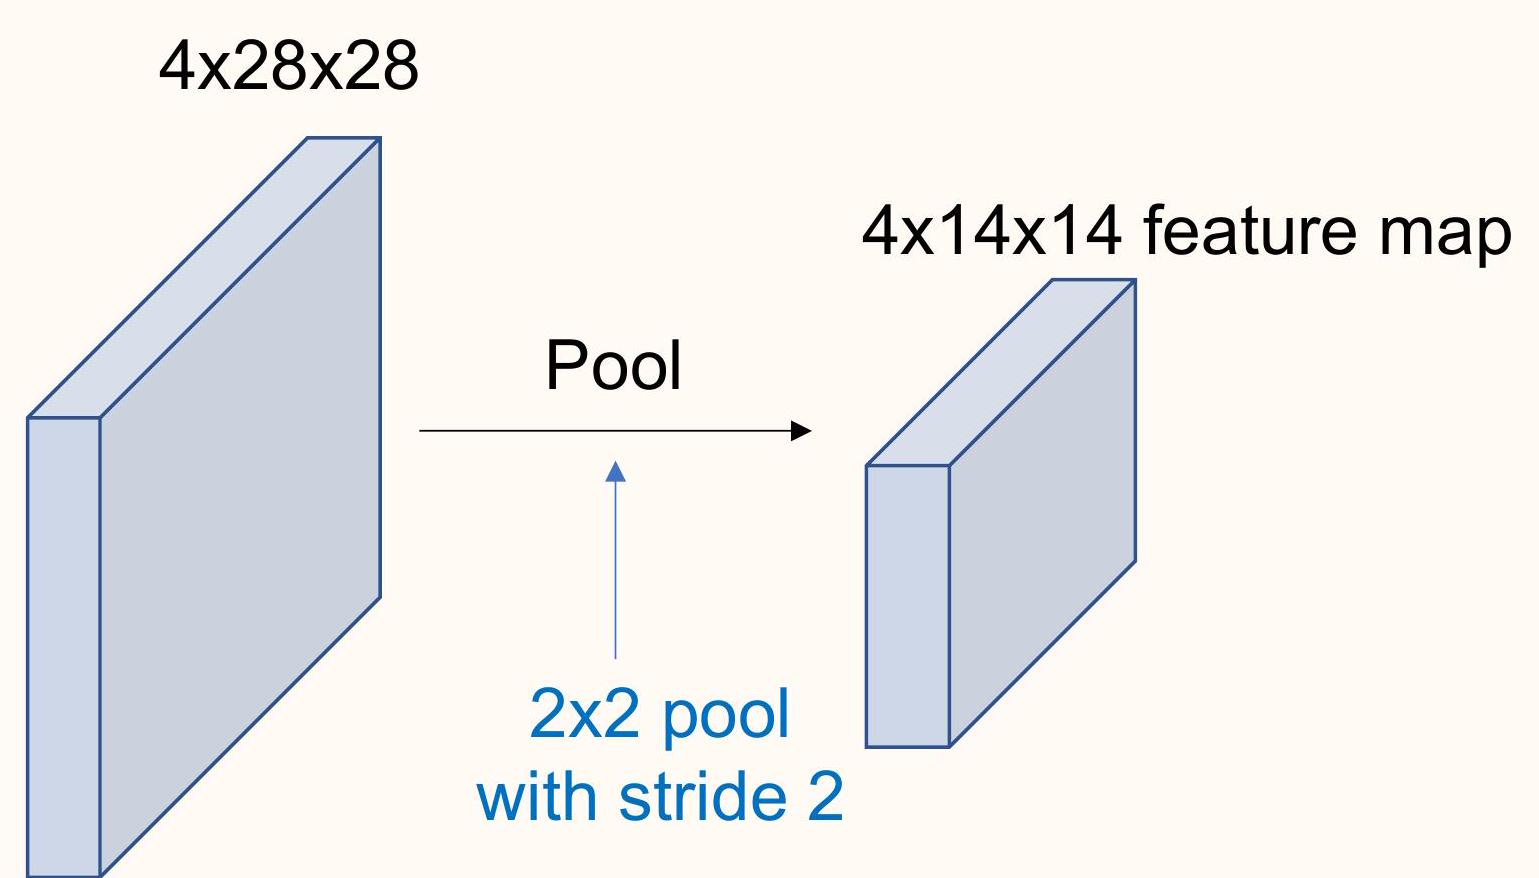
\includegraphics[width=0.5\textwidth]{.././assets/5.6.jpg}
    \end{figure}

    \begin{figure}[H]
        \centering
        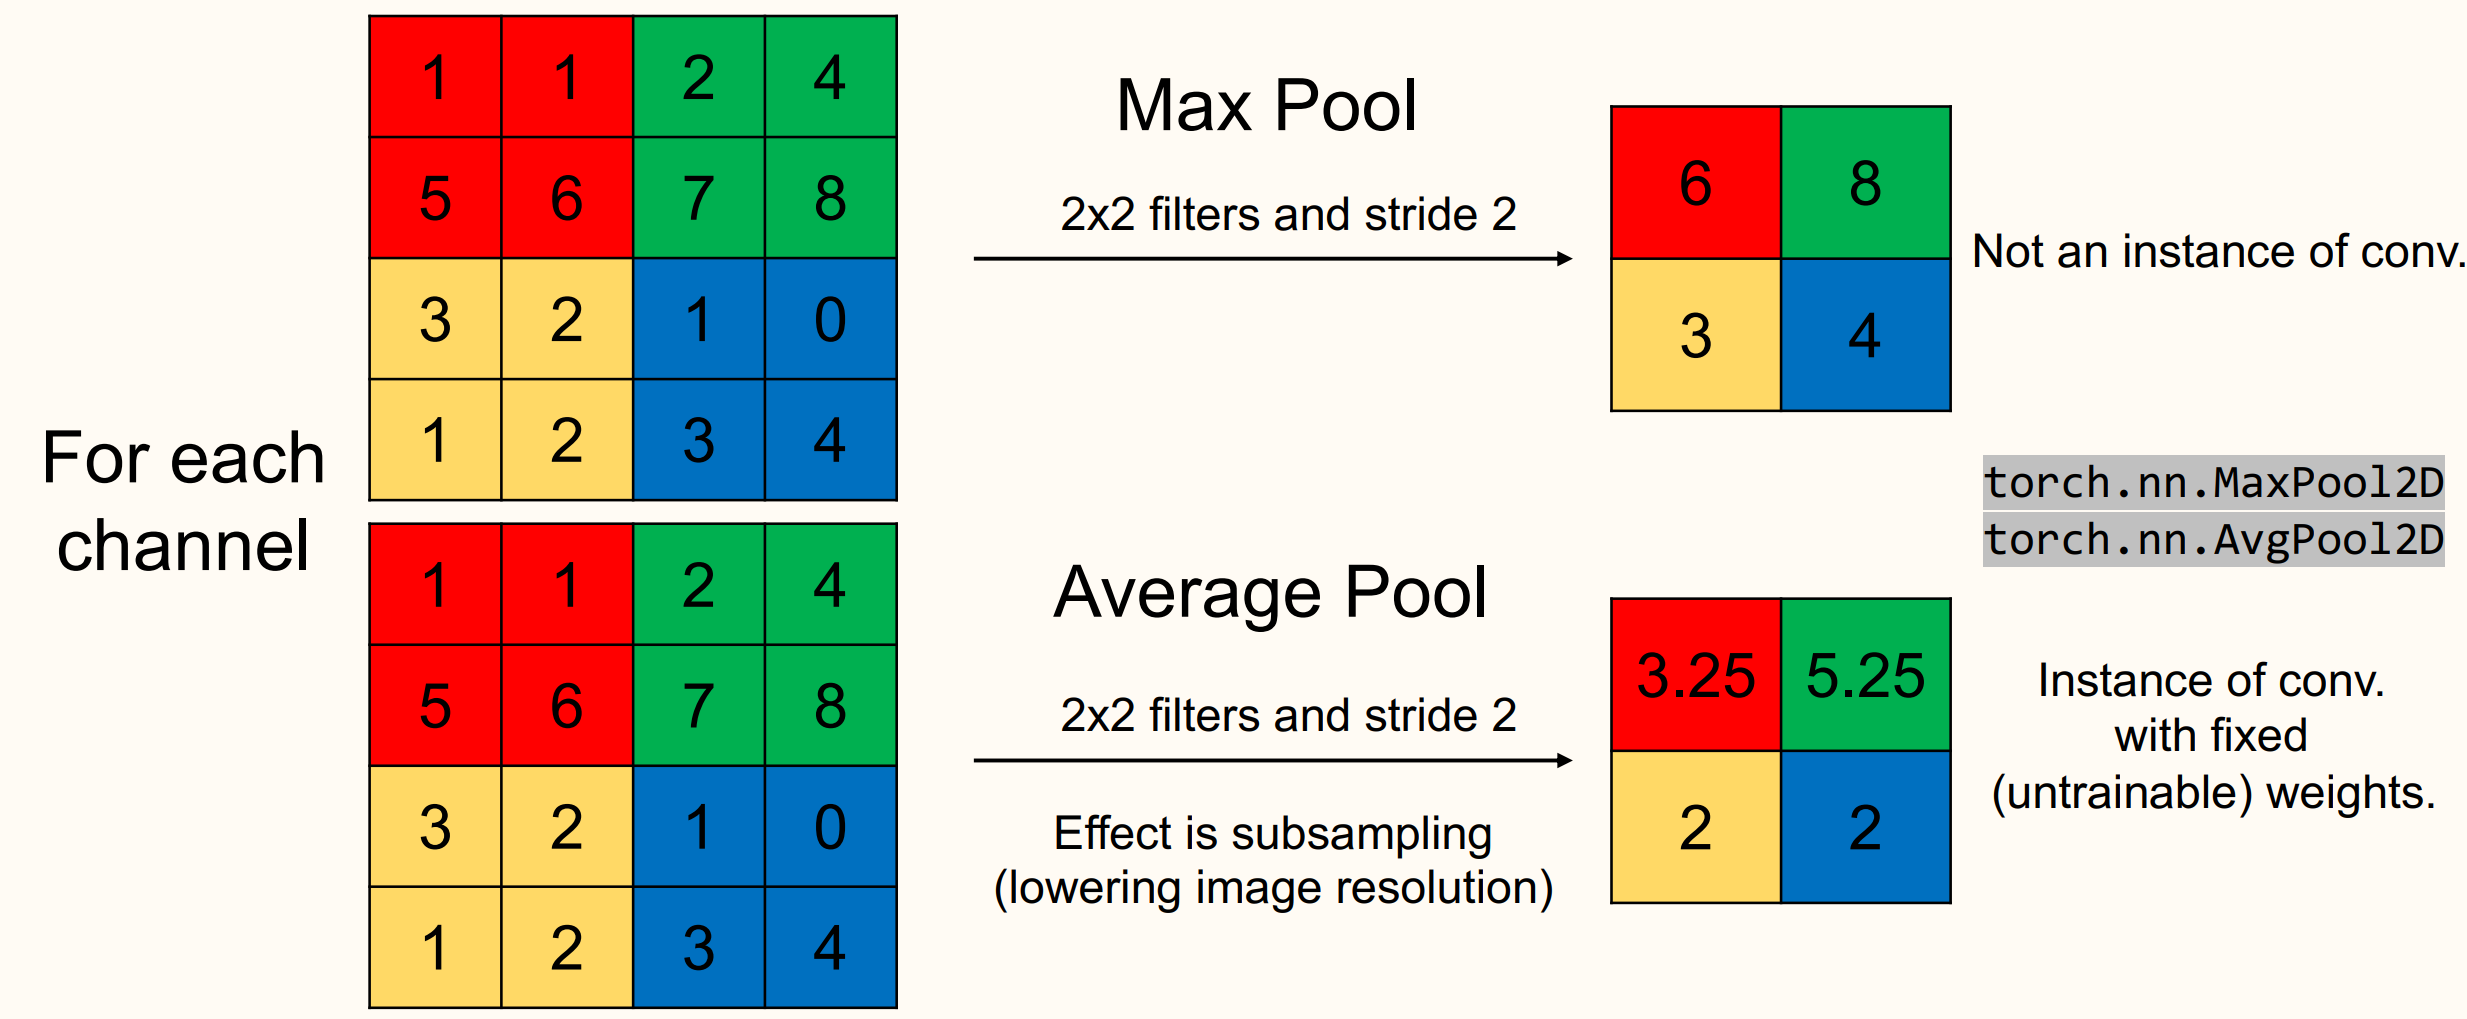
\includegraphics[width=1.0\textwidth]{.././assets/5.7.png}
    \end{figure}
\end{concept}

\begin{concept}[5.9][Weight Sharing]
    In neural networks, weight sharing is a way to reduce the number of parameters by reusing the same parameter in multiple operations. Convolutional layers are the primary example.

    $$
    A_{w}=\left[\begin{array}{cccccccc}
    w_{1} & \cdots & w_{r} & 0 & \cdots & & & 0 \\
    0 & w_{1} & \cdots & w_{r} & 0 & \cdots & & 0 \\
    0 & 0 & w_{1} & \cdots & w_{r} & 0 & \cdots & 0 \\
    \vdots & & & \ddots & & \ddots & & \vdots \\
    0 & & \cdots & 0 & w_{1} & \cdots & w_{r} & 0 \\
    0 & & \cdots & 0 & 0 & w_{1} & \cdots & w_{r}
    \end{array}\right]
    $$

    If we consider convolution with filter $w$ as a linear operator, the components of $w$ appear may times in the matrix representation.
    This is because the same $w$ is reused for every patch in the convolution.
    Weight sharing in convolution may now seem obvious, but it was a key contribution back when the LeNet architecture was presented.

    Some models (not studied in this course) use weight sharing more explicitly in other ways.
\end{concept}

\begin{concept}[5.10][Geometric Deep Learning]
    More generally, given a group $\mathcal{G}$ encoding a symmetry or invariance, one can define operations "equivariant" with respect $\mathcal{G}$ and construct equivariant neural networks.

    This is the subject of geometric deep learning, and its formulation utilizes graph theory and group theory.

    Geometric deep learning is particularly useful for non-Euclidean data. Examples include as protein molecule data and social network service connections.
\end{concept}

\chapter{Foundations of Design and Training of Deep Neural Networks}

\section{Data Augmentation}

\begin{definition}[6.1][Spurious Correlation]
    Hypothetical: A photographer prefers to take pictures with cats looking to the left and dogs looking to the right. Neural network learns to distinguish cats from dogs by which direction it is facing. This learned correlation will not be useful for pictures taken by another photographer.

    This is a \textbf{spurious correlation}, a correlation between the data and labels that does not capture the "true" meaning. Spurious correlations are not robust in the sense that the spurious correlation will not be a useful predictor when the data changes slightly.
\end{definition}

\begin{definition}[6.2][Data Augmentation (DA)]
    \begin{figure}[H]
        \centering
        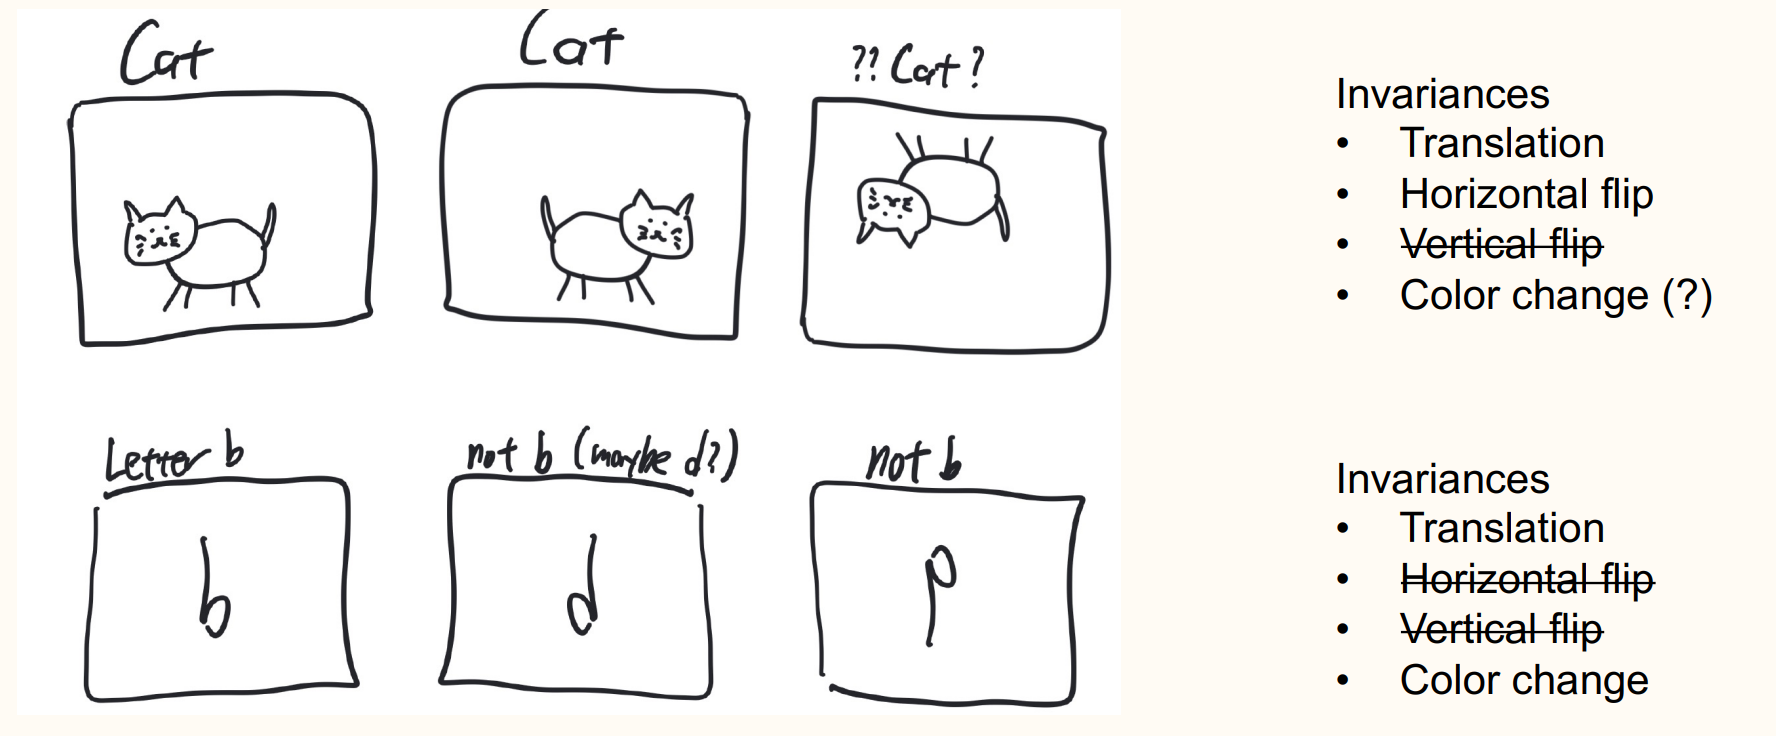
\includegraphics[width=1.0\textwidth]{.././assets/6.1.png}
    \end{figure}

    Translation invariance are encoded in convolution, but other invariances are harder to encode (unless one uses geometric deep learning).
    Therefore encode invariances in data and have neural networks learn the invariance.

    \par\noindent\textcolor{gray}{\hdashrule{\textwidth}{0.4pt}{1pt 2pt}}

    \textbf{Data augmentation (DA)} applies transforms to the data while preserving meaning and label.

    \begin{itemize}
        \item
        Option 1: Enlarge dataset itself.\\

        Usually cumbersome and unnecessary.
        \item
        Option 2: Use randomly transformed data in training loop.\\

        In PyTorch, we use \verb|Torchvision.transforms|.
    \end{itemize}

    \par\noindent\textcolor{gray}{\hdashrule{\textwidth}{0.4pt}{1pt 2pt}}

    We use DA to :

    \begin{itemize}
        \item Inject our prior knowledge of the structure of the data and force the neural network to learn it.
        \item Remove spurious correlations.
        \item Increase the effective data size. In particular, we ensure neural network never encounters the exact same data again and thereby prevent the neural network from performing exact memorization. (Neural network can memorize quite well.)
    \end{itemize}

    Effects of DA :

    \begin{itemize}
        \item DA usually worsens the training error (but we don't care about training error).
        \item
        DA often, but not always, improves the test error.\\

        If DA removes a spurious correlation, then the test error can be worsened.
        \item DA usually improves robustness.
    \end{itemize}
\end{definition}

\section{Overfitting \& Underfitting}

\begin{definition}[6.3][Classical Statistics - Overfitting vs Underfitting]
    \begin{figure}[H]
        \centering
        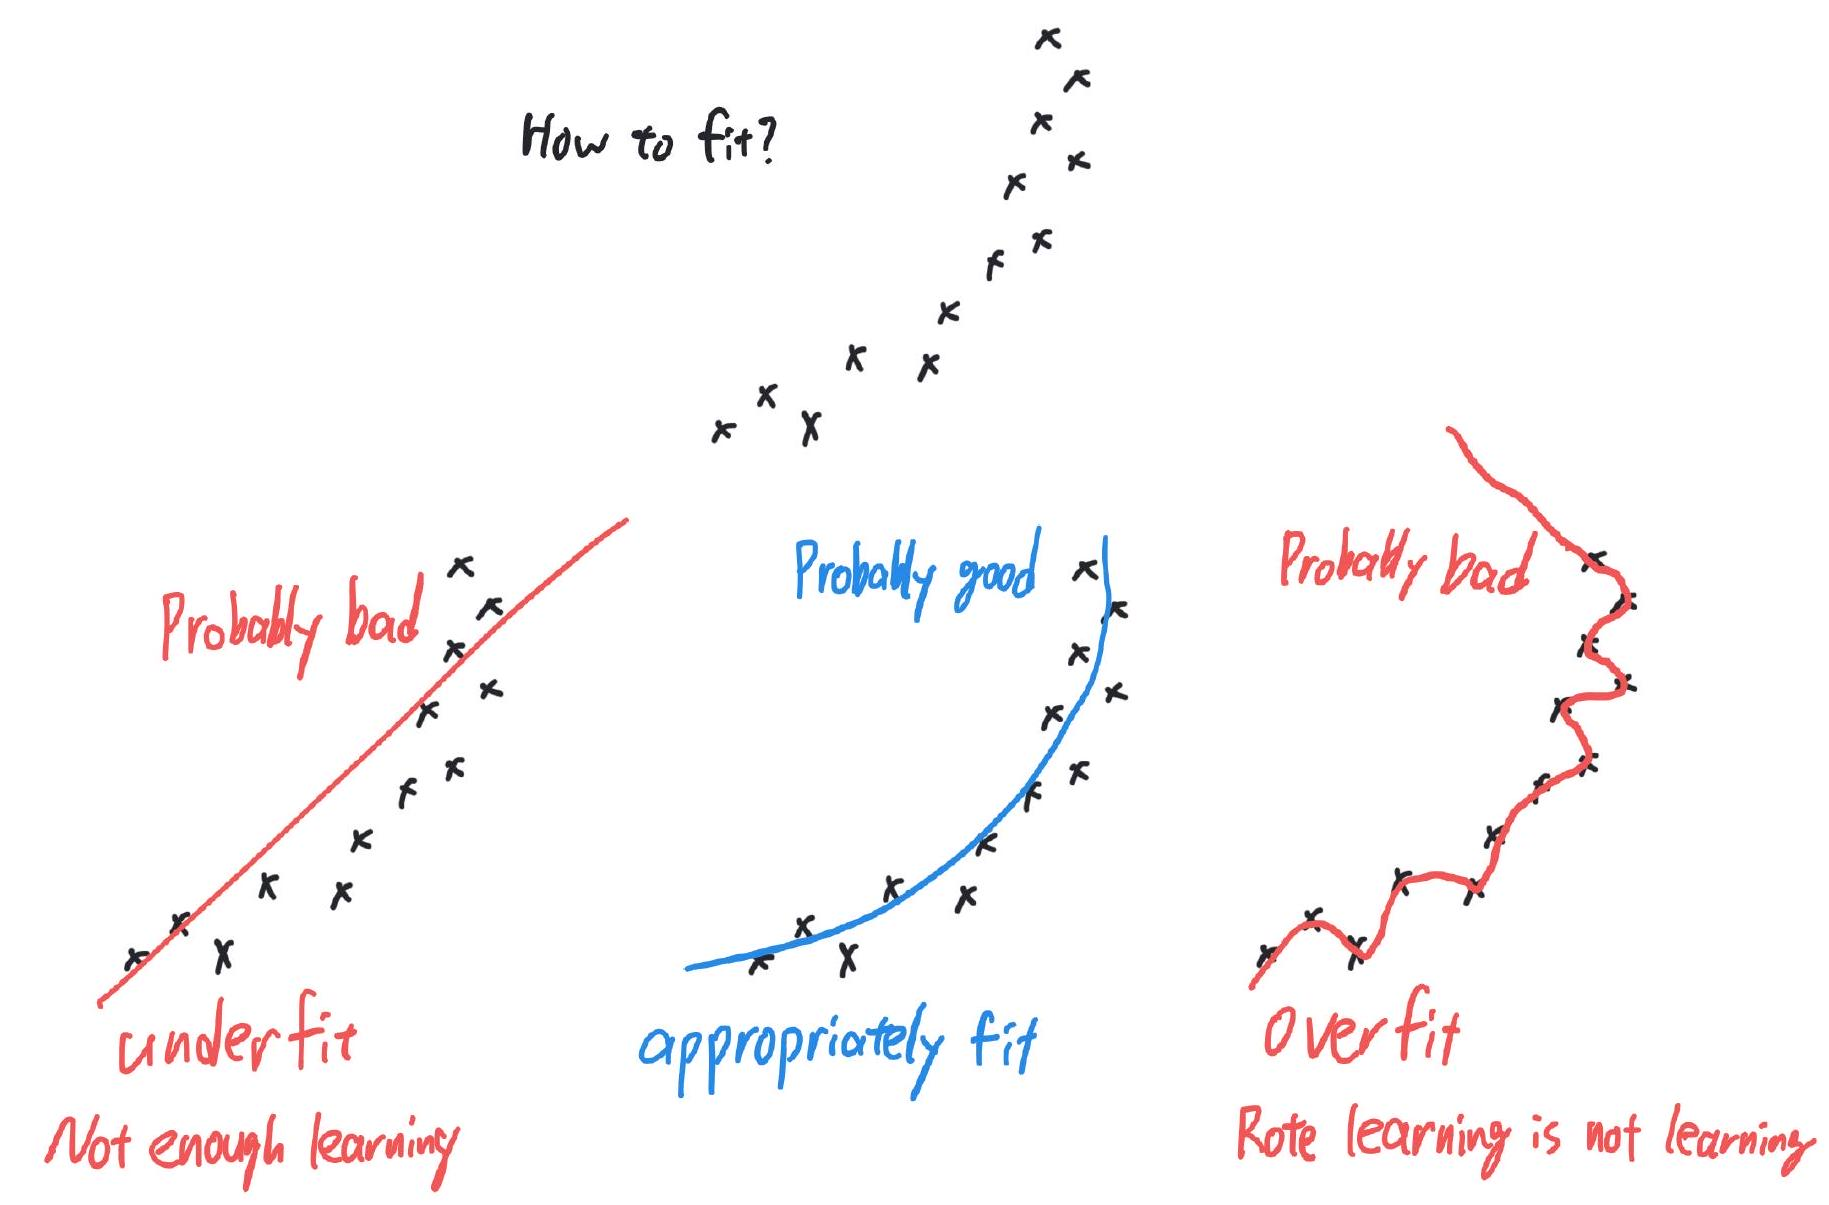
\includegraphics[width=0.8\textwidth]{.././assets/6.2.jpg}
    \end{figure}

    \begin{figure}[H]
        \centering
        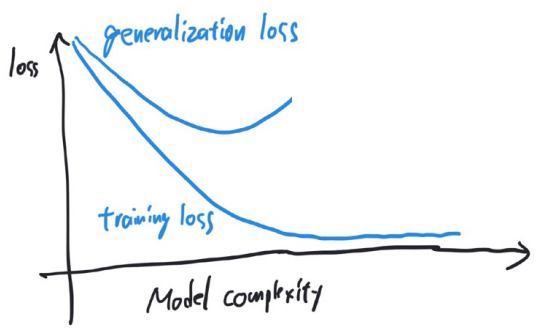
\includegraphics[width=0.6\textwidth]{.././assets/6.3.png}
    \end{figure}

    Given separate train and test data

    \begin{itemize}
        \item When (training loss) << (testing loss) you are \textbf{overfitting}. What you have learned from the training data does not carry over to test data.
        \item When (training loss) $\approx$ (testing loss) you are \textbf{underfitting}. You have the potential to learn more from the training data.
    \end{itemize}

    \par\noindent\textcolor{gray}{\hdashrule{\textwidth}{0.4pt}{1pt 2pt}}

    The goal of ML is to learn patterns that generalize to data you have not seen. From each datapoint, you want to learn enough (don't underfit) but if you learn too much you overcompensate for an observation specific to the single experience.

    In classical statistics, underfitting vs. overfitting (bias vs. variance tradeoff) is characterized rigorously.
\end{definition}

\begin{definition}[6.4][Modern Deep Learning - Double Descent]
    In modern deep learning, you can overfit, but the state-of-the art neural networks do not overfit (or "benignly overfit") despite having more model parameters than training data.

    We do not yet have clarity with this new phenomenon called \textbf{double descent}. When overfitting happens and when it does not is unclear.

    \begin{figure}[H]
        \centering
        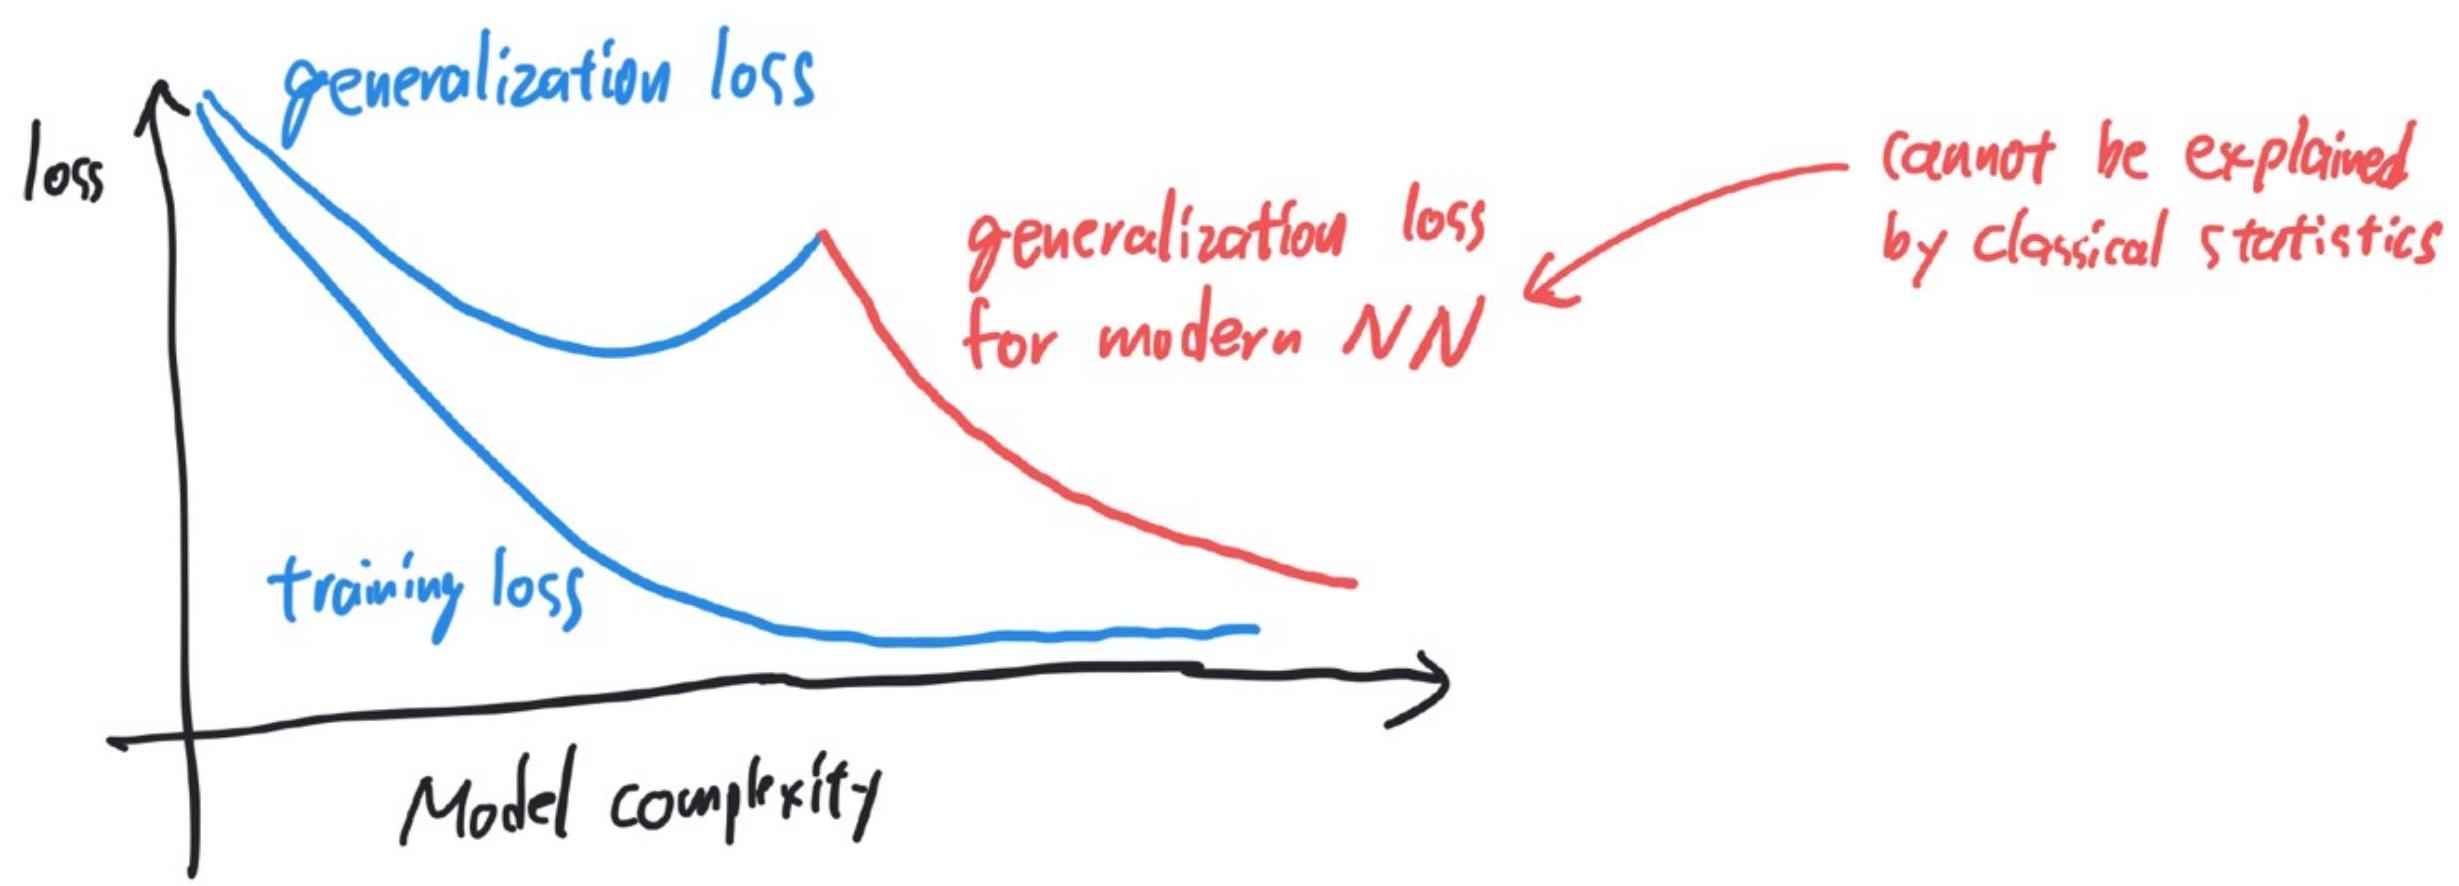
\includegraphics[width=1.0\textwidth]{.././assets/6.4.jpg}
    \end{figure}
\end{definition}

\begin{example}[6.5][Double Descent on 2-Layer Neural Network on MNIST]
    Belkin et al. experimentally demonstrates the double descent phenomenon with an MLP trained on the MNIST dataset.

    \begin{figure}[H]
        \centering
        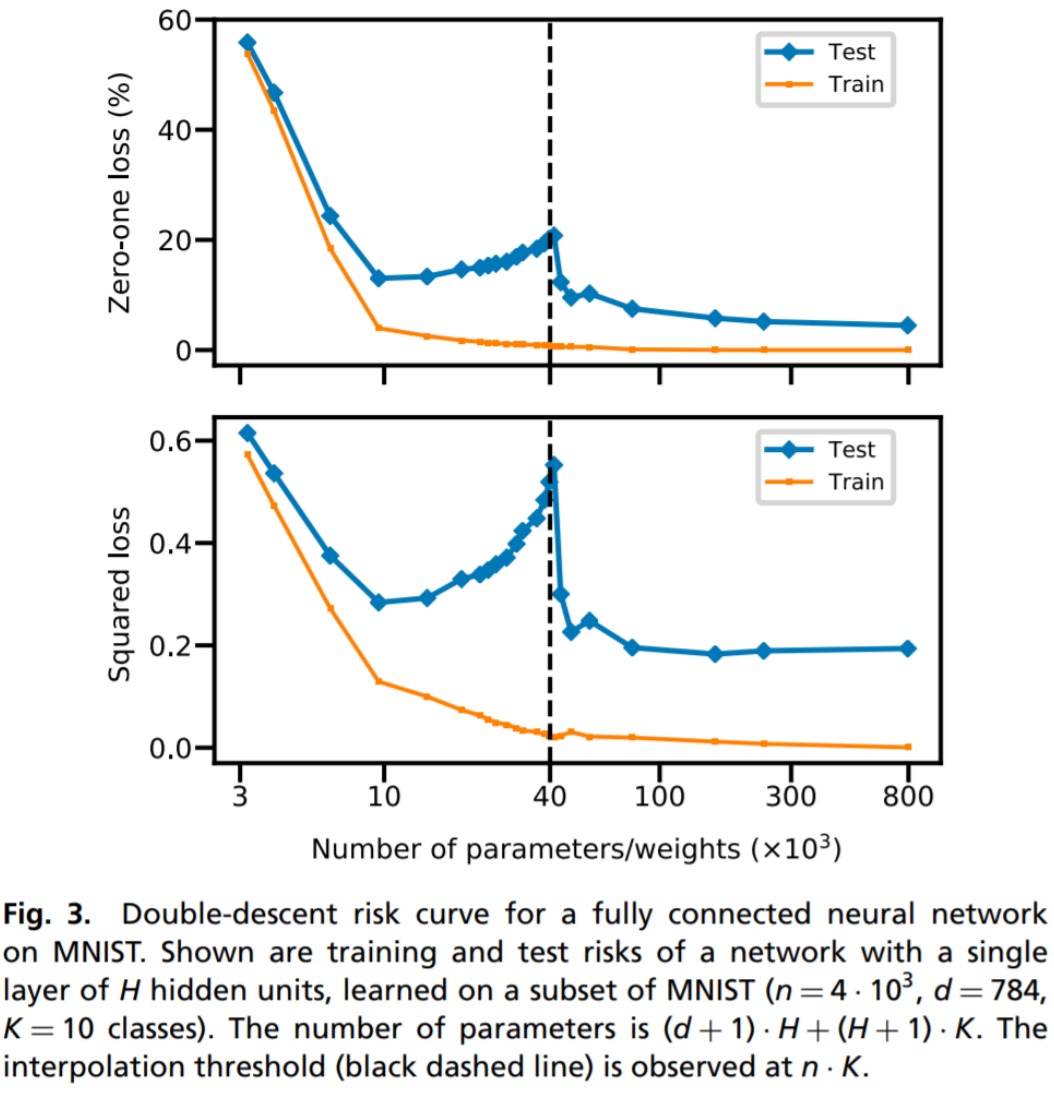
\includegraphics[width=0.6\textwidth]{.././assets/6.5.png}
    \end{figure}

    (M. Belkin, D. Hsu, S. Ma, and S. Mandal, Reconciling modern machine-learning practice and the classical bias-variance trade-off, PNAS, 2019.)
\end{example}

\begin{concept}[6.6][How to Avoid Overfitting]
    \textbf{Regularization} is loosely defined as mechanisms to prevent overfitting.

    When you are overfitting, regularize with:

    \begin{itemize}
        \item Smaller NN (fewer parameters) or larger NN (more parameters).
        \item
        Improve data by:

        \begin{itemize}
            \item using data augmentation
            \item acquiring better, more diverse, data
            \item acquiring more of the same data
        \end{itemize}
        \item Weight decay
        \item Dropout
        \item Early stopping on SGD or late stopping on SGD
    \end{itemize}
\end{concept}

\begin{concept}[6.7][How to Avoid Underfitting]
    When you are underfitting, use:

    \begin{itemize}
        \item Larger NN (if computationally feasible)
        \item Less weight decay
        \item Less dropout
        \item Run SGD longer (if computationally feasible)
    \end{itemize}
\end{concept}

\begin{concept}[6.8][Summary of Overfitting vs Underfitting]
    In modern deep learning, the double descent phenomenon has brought a conceptual and theoretical crisis regarding over and underfitting. Much of the machine learning practice is informed by classical statistics and learning theory, which do not take the double descent phenomenon into account.

    Double descent will bring fundamental changes to statistics, and researchers need more time to figure things out. Most researchers, practitioners and theoreticians, agree that not all classical wisdom is invalid, but what part do we keep, and what part do we replace?

    In the meantime, we will have to keep in mind the two contradictory viewpoints and move forward in the absence of clarity.
\end{concept}

\subsection{Weight Decay}

\begin{definition}[6.9][$\ell^{2}$ - Regularization]
    \textbf{$\ell^{2}$-regularization} augments the loss function with

    $$
    \underset{\theta \in \mathbb{R}^{p}}{\operatorname{minimize}} \frac{1}{N} \sum_{i=1}^{N} \ell\left(f_{\theta}\left(x_{i}\right), y_{i}\right)+\frac{\lambda}{2}\|\theta\|^{2}
    $$

    SGD on the augmented loss is usually implemented by changing SGD update rather than explicitly changing the loss since

    $$
    \begin{gathered}
    \theta^{k+1}=\theta^{k}-\alpha\left(g^{k}+\lambda \theta^{k}\right) \\
    =(1-\alpha \lambda) \theta^{k}-\alpha g^{k}
    \end{gathered}
    $$

    Where $g^{k}$ is stochastic gradient of original (unaugmented) loss.

    In classical statistics, this is called ridge regression or maximum a posteriori (MAP) estimation with Gaussian prior.
\end{definition}

\begin{concept}[6.10][Weight Decay $\cong \ell^{2}$ - Regularization]
    In Pytorch, you can use SGD + weight decay by:

    augmenting the loss function

    \begin{verbatim}
    for param in model.parameters():
        loss += (lamda/2)*param.pow(2.0).sum()
    torch.optim.SGD(model.parameters(), lr=... , weight_decay=0)
    \end{verbatim}

    or by using \verb|weight_decay| in the optimizer

    \begin{verbatim}
    torch.optim.SGD(model.parameters(), lr=... , weight_decay=lamda)
    \end{verbatim}

    \par\noindent\textcolor{gray}{\hdashrule{\textwidth}{0.4pt}{1pt 2pt}}

    For plain SGD, weight decay and $\ell^{2}$-regularization are equivalent. For other optimizers, the two are similar but not the same. More on this later.
\end{concept}

\subsection{Dropout}

\begin{definition}[6.11][Dropout]
    Dropout is a regularization technique that randomly disables neurons.

    Standard layer,

    $$
    h_{2}=\sigma\left(W_{1} h_{1}+b_{1}\right)
    $$

    Dropout with drop probability $p$ defines

    $$
    h_{2}=\sigma\left(W_{1} h_{1}^{\prime}+b_{1}\right)
    $$

    with $h_{1}^{\prime}$ defined as

    $$
    \left(h_{1}^{\prime}\right)_{j}= \begin{cases}0 & \text { with probability } p \\ \frac{\left(h_{1}\right)_{j}}{1-p} & \text { otherwise }\end{cases}
    $$

    Note that $h_{1}^{\prime}$ is defined so that $\mathbb{E}[h_{1}^{\prime}]=h_1$.

    \begin{figure}[H]
        \centering
        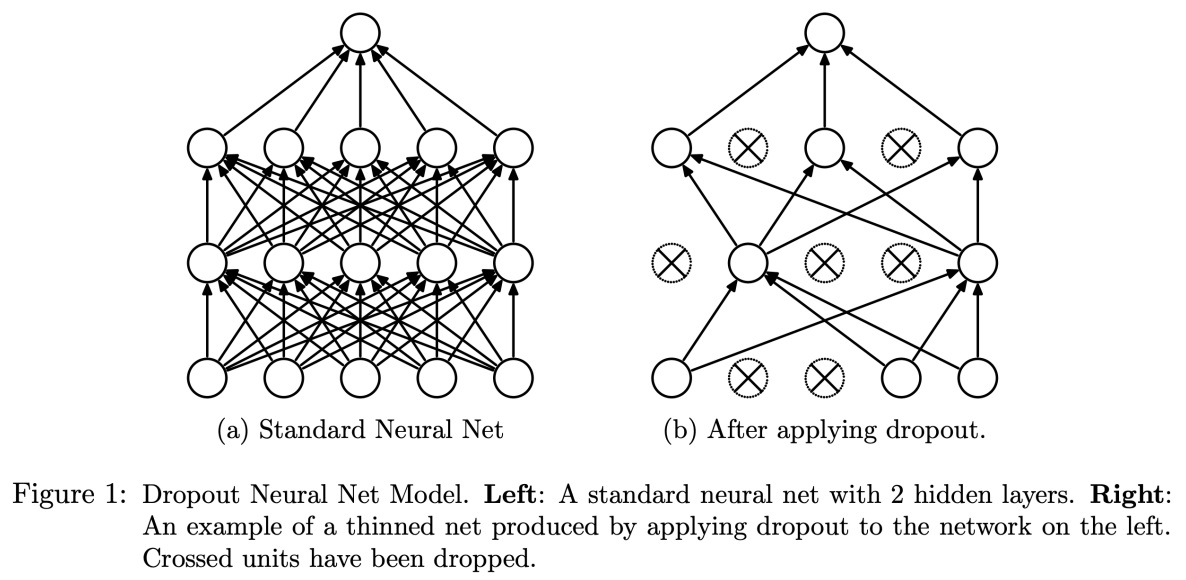
\includegraphics[width=0.8\textwidth]{.././assets/6.6.png}
    \end{figure}

    During training, dropout masks are different in every forward pass due to their random nature.

    (N. Srivastava, G. Hinton, A. Krizhevsky, I. Sutskever, R. Salakhutdinov, Dropout: A Simple Way to Prevent Neural Networks from Overfitting, JMLR, 2014.)
\end{definition}

\begin{concept}[6.12][Why is dropout helpful?]
    "A motivation for dropout comes from a theory of the role of sex in evolution (Livnat et al., 2010)."

    Sexual reproduction, compared to asexual reproduction, creates the criterion for natural selection mix-ability of genes rather than individual fitness, since genes are mixed in a more haphazard manner.

    "Since a gene cannot rely on a large set of partners to be present at all times, it must learn to do something useful on its own or in collaboration with a small number of other genes. ... Similarly, each hidden unit in a neural network trained with dropout must learn to work with a randomly chosen sample of other units. This should make each hidden unit more robust and drive it towards creating useful features on its own without relying on other hidden units to correct its mistakes.

    The analogy to evolution is very interesting, but it is ultimately a heuristic argument. It also shifts the burden to the question: "why is sexual evolution more powerful than asexual evolution?"

    However, dropout can be shown to be loosely equivalent to $\ell^{2}$-regularization. However, we do not yet have a complete understanding of the mathematical reason behind dropout's performance.
\end{concept}

\begin{concept}[6.13][Dropout in Pytorch]
    Dropout simply multiplies the neurons with a random $0-\frac{1}{1-p_{\text {drop }}}$ mask.

    A direct implementation in PyTorch:

    \begin{verbatim}
    def dropout_layer(X, p_drop):
        mask = (torch.rand(X.shape) > p_drop).float()
        return mask * X / (1.0 - p_drop)
    \end{verbatim}

    PyTorch provides an implementation of dropout through \verb|torch.nn.Dropout|.
\end{concept}

\begin{concept}[6.14][Dropout in Training vs Test]
    Typically, dropout is used during training and turned off during prediction/testing.
    (Dropout should be viewed as an additional onus imposed during training to make training more difficult and thereby effective, but it is something that should be turned off later.)

    In PyTorch, activate the training mode with

    \begin{verbatim}
    model.train()
    \end{verbatim}

    and activate evaluation mode with

    \begin{verbatim}
    model.eval()
    \end{verbatim}

    dropout (and batchnorm) will behave differently in these two modes.
\end{concept}

\begin{concept}[6.15][When to Use Dropout]
    Dropout is usually used on linear layers but not on convolutional layers.

    \begin{itemize}
        \item Linear layers have many weights and each weight is used only once per forward pass. (If $y=\operatorname{Linear}_{A, b}(x)$, then $A_{i j}$ only affect $y_{i}$.) So regularization seems more necessary.
        \item A convolutional filter has fewer weights and each weight is used multiple times in each forward pass. (If $y=\operatorname{Conv} 2 \mathrm{D}_{w, b}(x)$, then $w_{i j k t}$ affects $\left.y_{i, .,:}.\right)$ So regularization seems less necessary.
    \end{itemize}

    Dropout seems to be going out of fashion:

    \begin{itemize}
        \item Dropout's effect is somehow subsumed by batchnorm. (This is poorly understood.)
        \item Linear layers are less common due to their large number of trainable parameters.
    \end{itemize}

    There is no consensus on whether dropout should be applied before or after the activation function. However, Dropout- $\sigma$ and $\sigma$-Dropout are equivalent when $\sigma$ is $\operatorname{ReLU}$ or leaky $\operatorname{ReLU}$, or, more generally, when $\sigma$ is nonnegative homogeneous.
\end{concept}

\subsection{SGD Early / Late Stopping}

\begin{definition}[6.16][SGD Early Stopping]
    \textbf{Early stopping of SGD} refers to stopping the training early even if you have time for more iterations.

    The rationale is that SGD fits data, so too many iterations lead to overfitting.

    A similar phenomenon (too many iterations hurt) is observed in classical algorithms for inverse problems.

    \begin{figure}[H]
        \centering
        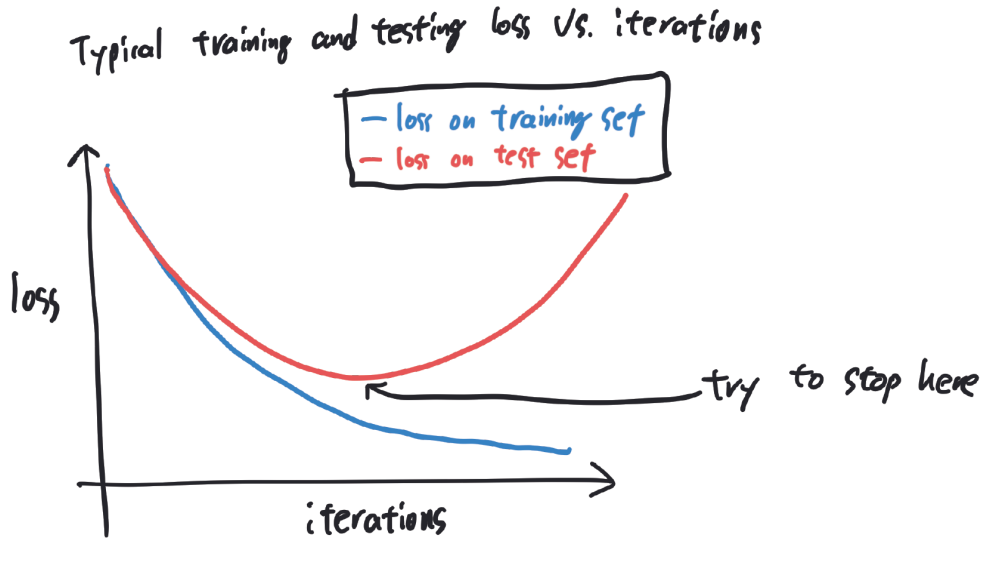
\includegraphics[width=0.75\textwidth]{.././assets/6.7.png}
    \end{figure}
\end{definition}

\begin{definition}[6.17][Epochwise Double Descent]
    Recently, however, an \textbf{epochwise double descent} has been observed.

    So perhaps one should stop SGD early or very late.

    We do not yet have clarity with this new phenomenon.

    \begin{figure}[H]
        \centering
        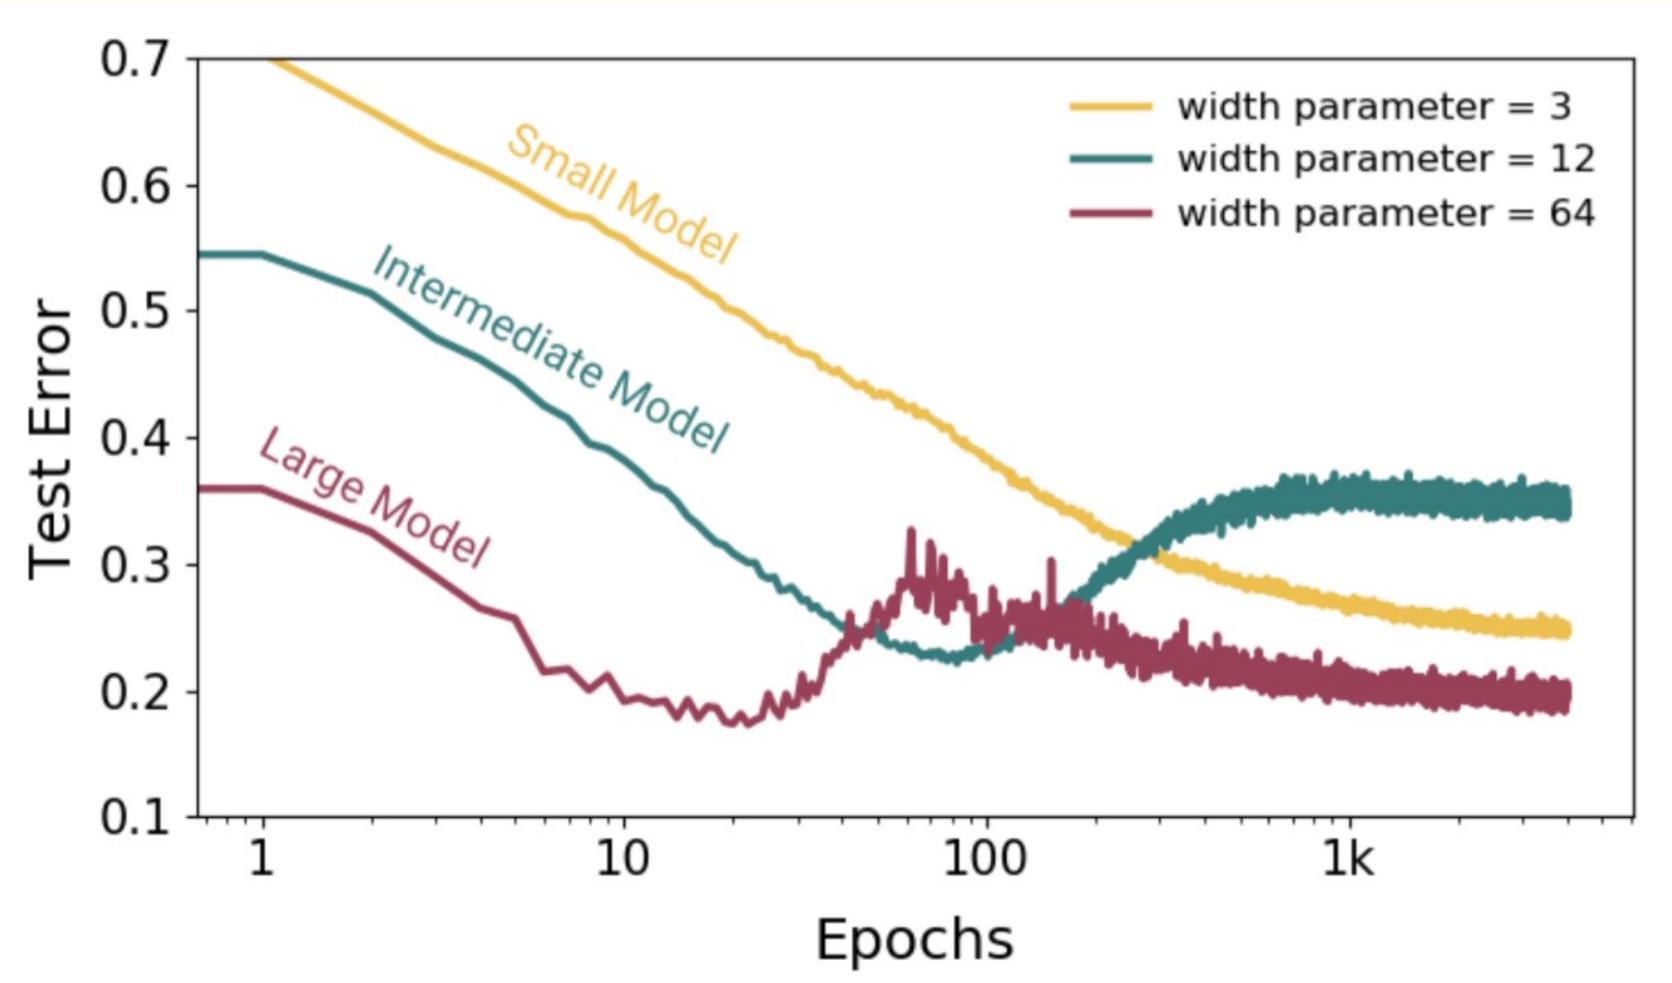
\includegraphics[width=0.75\textwidth]{.././assets/6.8.jpg}
    \end{figure}

    (P. Nakkiran, G. Kaplun, Y. Bansal, T. Yang, B. Barak, and I. Sutskever, Deep double descent: Where bigger models and more data hurt, ICLR, 2020.)
\end{definition}

\subsection{More Data}

\begin{concept}[6.18][More Data (by Data Augmentation)]
    With all else fixed, using more data usually leads to less overfitting.

    However, collecting more data is often expensive.

    Think of data augmentation (DA) as a mechanism to create more data for free. You can view DA as a form of regularization.
\end{concept}

\section{SGD Optimizer}

\begin{definition}[6.19][SGD with Momentum]
    SGD:

    $$
    \theta^{k+1}=\theta^{k}-\alpha g^{k}
    $$

    \textbf{SGD with momentum}:

    $$
    \begin{gathered}
    v^{k+1}=g^{k}+\beta v^{k} \\
    \theta^{k+1}=\theta^{k}-\alpha v^{k+1}
    \end{gathered}
    $$

    $\beta=0.9$ is a common choice.

    \begin{figure}[H]
        \centering
        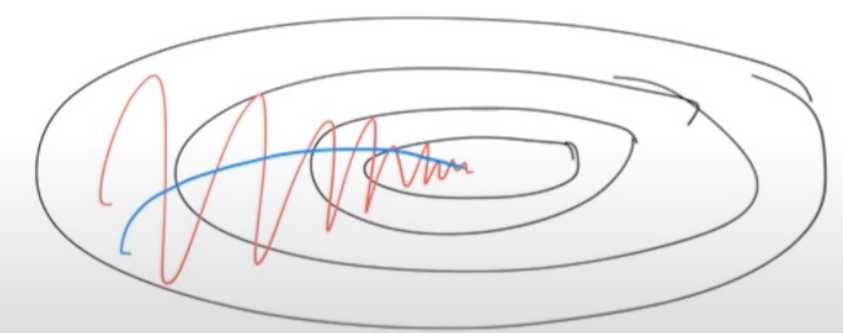
\includegraphics[width=0.5\textwidth]{.././assets/6.9.png}
    \end{figure}

    When different coordinates (parameters) have very different scalings (i.e., when the problem is ill-conditioned, momentum can help find a good direction of progress.

    (I. Sutskever, J. Martens, G. Dahl, and G. Hinton, On the importance of initialization and momentum in deep learning, ICML, 2013.)
\end{definition}

\begin{definition}[6.20][RMSProp]
    \textbf{RMSProp}:

    $$
    \begin{gathered}
    m_{2}^{k+1}=\beta_{2} m_{2}^{k}+\left(1-\beta_{2}\right)\left(g^{k} \circledast g^{k}\right) \\
    \theta^{k+1}=\theta^{k}-\alpha g^{k} \oslash \sqrt{m_{2}^{k+1}+\epsilon}
    \end{gathered}
    $$

    $\beta_{2}=0.99$ and $\epsilon=10^{-8}$ are common values. $\circledast$ and $\oslash$ are elementwise mult. and div.

    $m_{2}^{k}$ is a running estimate of the $2^{\text {nd }}$ moment of the stochastic gradients, i.e., $\left(m_{2}^{k}\right)_{i} \approx \mathbb{E}\left(g^{k}\right)_{i}^{2}$.

    $\alpha \oslash \sqrt{m_{2}^{k+1}+\epsilon}$ is the learning rate scaled elementwise. Progress along steep and noisy directions are dampened while progress along flat and non-noisy directions are accelerated.

    (T. Tieleman, and G. Hinton, Lecture 6.5 - RMSProp, COURSERA: Neural Networks for Machine Learning, 2012.)
\end{definition}

\begin{definition}[6.21][Adam (Adaptive Moment Estimation)]
    \textbf{Adam}:

    $$
    \begin{gathered}
    m_{1}^{k+1}=\beta_{1} m_{1}^{k}+\left(1-\beta_{1}\right) g^{k}, m_{2}^{k+1}=\beta_{2} m_{2}^{k}+\left(1-\beta_{2}\right)\left(g^{k} \circledast g^{k}\right) \\
    \tilde{m}_{1}^{k+1}=\frac{m_{1}^{k+1}}{1-\beta_{1}^{k+1}}, \quad \widetilde{m}_{2}^{k+1}=\frac{m_{2}^{k+1}}{1-\beta_{2}^{k+1}} \\
    \theta^{k+1}=\theta^{k}-\alpha \widetilde{m}_{1}^{k+1} \oslash \sqrt{\widetilde{m}_{2}^{k+1}+\epsilon}
    \end{gathered}
    $$

    \begin{itemize}
        \item $\beta_{1}^{k+1}$ means $\beta_{1}$ to the $(k+1)$ th power.
        \item $\beta_{1}=0.9, \beta_{2}=0.999$, and $\epsilon=10^{-8}$ are common values. Initialize with $m_{1}^{0}=m_{2}^{0}=0$.
        \item $m_{1}^{k}$ and $m_{2}^{k}$ are running estimates of the $1^{\text {st }}$ and $2^{\text {nd }}$ moments of $g^{k}$.
        \item $\tilde{m}_{1}^{k}$ and $\tilde{m}_{2}^{k}$ are bias-corrected estimates of $m_{1}^{k}$ and $m_{2}^{k}$.
        \item Using $\widetilde{m}_{1}^{k}$ instead of $g^{k}$ adds the effect of momentum.
    \end{itemize}

    (D. P. Kingma and J. Ba, Adam: A method for stochastic optimization, ICLR, 2015.)
\end{definition}

\begin{concept}[6.22][Bias correction of Adam]
    To understand the bias correction, consider the hypothetical $g^{k}=g$ for $k=0,1, \ldots$. Then

    $$
    \begin{gathered}
    m_{1}^{k}=\left(1-\beta_{1}^{k}\right) g \\
    m_{2}^{k}=\left(1-\beta_{2}^{k}\right)(g \circledast g)
    \end{gathered}
    $$

    Even though $m_{1}^{k} \rightarrow g$ and $m_{2}^{k} \rightarrow(g \circledast g)$ as $k \rightarrow \infty$, the estimators are not exact despite there being no variation in $g^{k}$.

    On the other hand, the bias-corrected estimators are exact:

    $$
    \begin{gathered}
    \widetilde{m}_{1}^{k}=g \\
    \widetilde{m}_{2}^{k}=(g \circledast g)
    \end{gathered}
    $$
\end{concept}

\begin{concept}[6.23][The Cautionary Tale of Adam]
    Adam's original 2015 paper justified the effectiveness of the algorithm through experiments training deep neural networks with Adam. After all, this non-convex optimization is what Adam was proposed to do.

    However, the paper also provided a convergence proof under the assumption of convexity. This was perhaps unnecessary in an applied paper focusing on non-convex optimization.

    The proof was later shown to be incorrect! Adam does not always converge in the convex setup, i.e., the algorithm, rather than the proof, is wrong.

    Reddi and Kale presented the AMSGrad optimizer, which does come with a correct convergence proof, but AMSGrad tends to perform worse than Adam, empirically.

    (S. J. Reddi, S. Kale, and S. Kumar, On the convergence of Adam and beyond, ICLR, 2018.)
\end{concept}

\begin{concept}[6.24][How to Choose Optimizer]
    Extensive research has gone into finding the "best" optimizer. Schmidt et al.${ }^{\star}$ reports that, roughly speaking, that Adam works well most of the time.

    \textbf{So, Adam is a good default choice. Currently, it seems to be the best default choice.}

    However, Adam does not always work. For example, it seems to be that the widely used EfficientNet model can only be trained ${ }^{\dagger}$ with RMSProp.

    However, there are some setups where the LR of SGD is harder to tune, but SGD outperforms Adam when properly tuned.${ }^{\#}$

    (${ }^{\star}$ R. M. Schmidt, F. Schneider, and P. Hennig, Descending through a crowded valley — benchmarking deep learning optimizers, ICML, 2021.\\
    ${ }^{\dagger}$ M. Tan and Q. V. Le, EfficientNet: Rethinking model scaling for convolutional neural networks, ICML, 2019.\\
    ${ }^{\#}$ A. C. Wilson, R. Roelofs, M. Stern, N. Srebro, and B. Recht, The marginal value of adaptive gradient methods in machine learning, NeurlPS, 2017.)
\end{concept}

\begin{concept}[6.25][How to Tune Parameters]
    Everything should be chosen by trial and error. The weight parameters and $\beta, \beta_{1}, \beta_{2}$ and the weight decay parameter $\lambda$, and the optimizers should be chosen based on trial and error.

    The LR (the stepsize $\alpha$ ) of different optimizers are not really comparable between the different optimizers. When you change the optimizer, the LR should be tuned again.

    Roughly, large stepsize, large momentum, small weight decay is faster but less stable, while small stepsize, small momentum, and large weight decay is slower but more stable.
\end{concept}

\begin{concept}[6.26][Using Different Optimizers in Pytorch]
    In PyTorch, the \verb|torch.optim| module implements the commonly used optimizers.

    \begin{itemize}
        \item Using SGD:
    \end{itemize}

    \begin{verbatim}
    torch.optim.SGD(model.parameters(), lr=X)
    \end{verbatim}

    \begin{itemize}
        \item Using SGD with momentum:
    \end{itemize}

    \begin{verbatim}
    torch.optim.SGD(model.parameters(), momentum=0.9, lr=X)
    \end{verbatim}

    \begin{itemize}
        \item Using RMSprop:
    \end{itemize}

    \begin{verbatim}
    torch.optim.RMSprop(model.parameters(), lr=X)
    \end{verbatim}

    \begin{itemize}
        \item Using Adam:
    \end{itemize}

    \begin{verbatim}
    torch.optim.Adam(model.parameters(), lr=X)
    \end{verbatim}
\end{concept}

\begin{concept}[6.27][Learning Rate Scheduling]
    Sometimes, it is helpful to change (usually reduce) the learning rate as the training progresses. PyTorch provides learning rate schedulers to do this.

    \begin{verbatim}
    optimizer = SGD(model.parameters(), lr=0.1)
    scheduler = ExponentialLR(optimizer, gamma=0.9) # lr = 0.9*lr
    for _ in range(...):
        for input, target in dataset:
            optimizer.zero_grad()
            output = model(input)
            loss = loss_fn(output, target)
            loss.backward()
            optimizer.step()
        scheduler.step() # .step() call updates (changes) the learning rate
    \end{verbatim}

    \par\noindent\textcolor{gray}{\hdashrule{\textwidth}{0.4pt}{1pt 2pt}}

    One common choice is to specify a diminishing learning rate via a function (a lambda expression). Choices like \verb|C/epoch| or \verb|C / sqrt(iteration)|, where \verb|C| is an appropriately chosen constant, are common.

    \begin{verbatim}
    # lr_lambda allows us to set lr with a function
    scheduler = LambdaLR(optimizer, lr_lambda = lambda ep: 1e-2/ep)
    for epoch in range(...):
        for input, target in dataset:
            optimizer.zero_grad()
            output = model(input)
            loss = loss_fn(output, target)
            loss.backward()
            optimizer.step()
        scheduler.step() # lr=0.01/epoch
    \end{verbatim}
\end{concept}

\begin{concept}[6.28][Cosine Learning Rate]
    The cosine learning rate scheduler, which sets the learning rate with the cosine function, is also commonly used.

    The $2^{\text {nd }}$ case in the specification means $k$ and its purpose is to prevent the learning rate from becoming 0 .

    It is also common to use only a half-period of the cosine rather than having the learning rate oscillate.

    \begin{figure}[H]
        \centering
        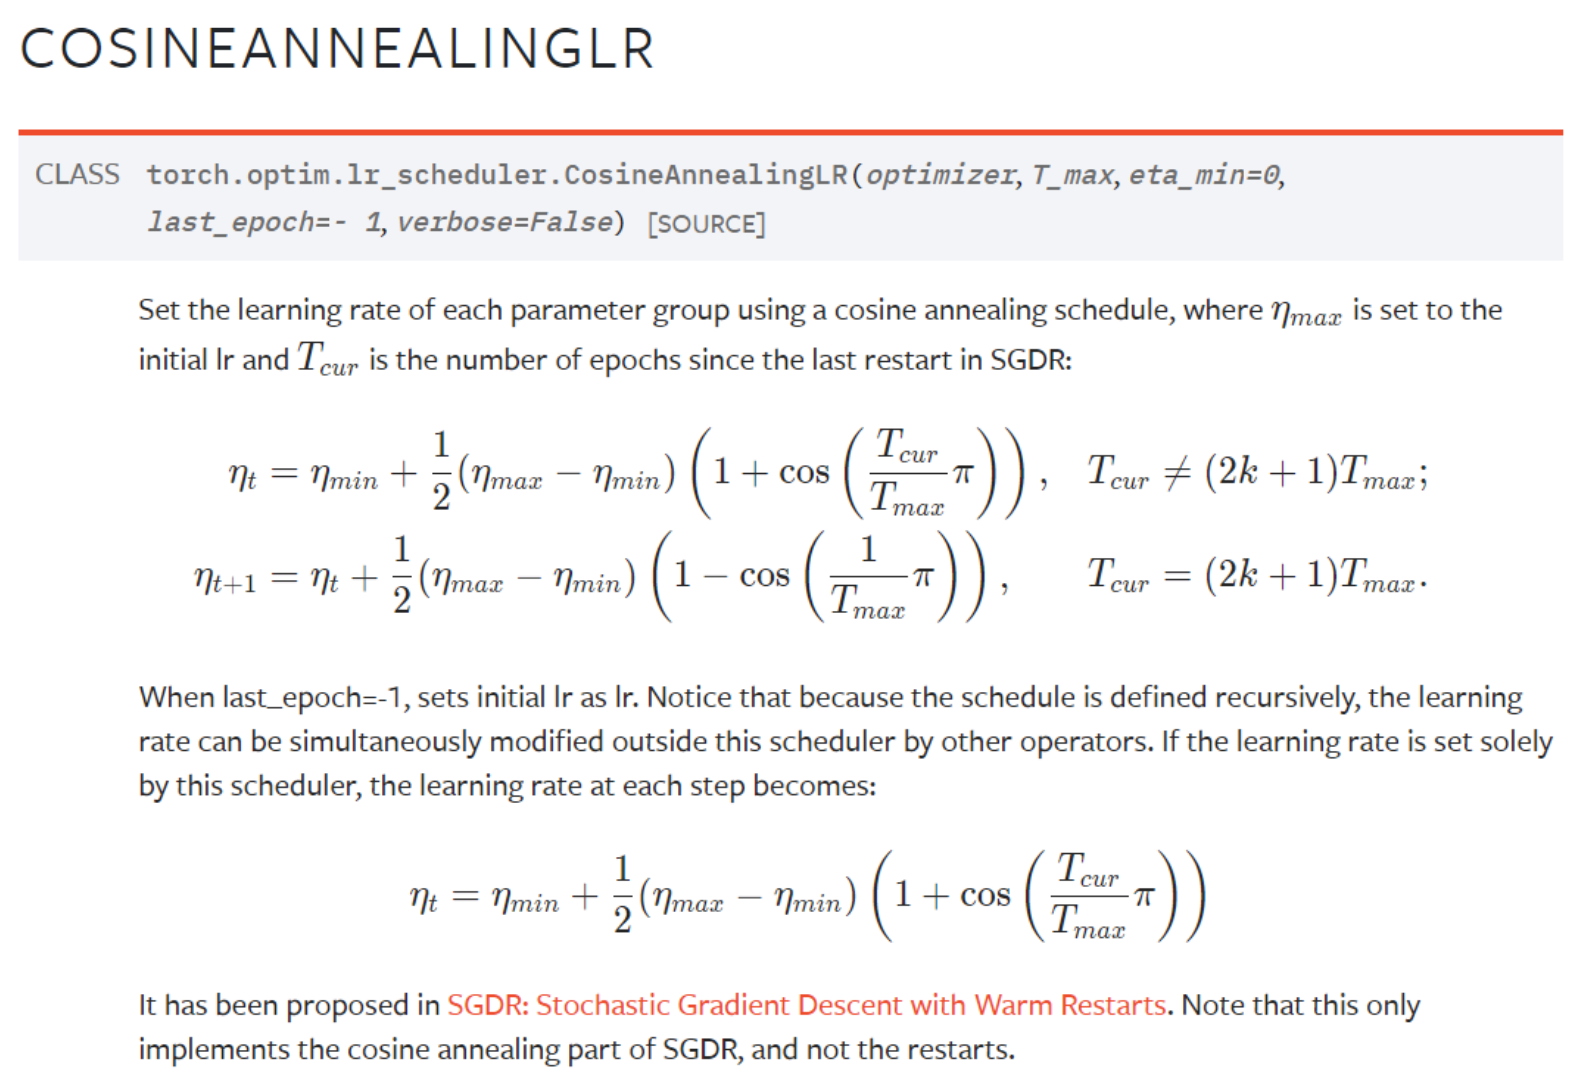
\includegraphics[width=0.8\textwidth]{.././assets/6.10.png}
    \end{figure}

    (I. Loshchilov and F. Hutter, SGDR: Stochastic gradient descent with warm restarts, ICLR, 2017)
\end{concept}

\begin{concept}[6.29][Wide vs Sharp Minima]
    \begin{itemize}
        \item Large step makes large and rough progress towards regions with small loss.
        \item Small steps refines the model by finding sharper minima.
    \end{itemize}

    Also small steps better suppress the effect of noise. Mathematically, one can show that SGD with small steps becomes very similar to GD with small steps.${ }^{\#}$

    However, using small steps to converge to sharp minima may not always be optimal. There is some empirical evidence that wide minima have better test error than sharp minima.${ }^{\star}$

    (${ }^{\#}$ D. Davis, D. Drusvyatskiy, S. Kakade and J. D. Lee, Stochastic subgradient method converges on tame functions, Found. Comput. Math., 2020.\\
    ${ }^{\star}$ Y. Jiang, B. Neyshabur, H. Mobahi, D. Krishnan, and S. Bengio, Fantastic generalization measures and where to find them, ICLR, 2020.)
\end{concept}

\section{Weight Initialization}

\begin{concept}[6.30][Importance of Weight Initialization]
    Remember, SGD is

    $$
    \theta^{k+1}=\theta^{k}-\alpha g^{k}
    $$

    where $\theta^{0} \in \mathbb{R}^{p}$ is an initial point. Using a good initial point is important in NN training.

    Prescription by LeCun et al.: "Weights should be chosen randomly but in such a way that the [tanh] is primarily activated in its linear region. If weights are all very large then the [tanh] will saturate resulting in small gradients that make learning slow. If weights are very small then gradients will also be very small." (Cf. Vanishing gradient)

    "Intermediate weights that range over the [tanh's] linear region have the advantage that (1) the gradients are large enough that learning can proceed and (2) the network will learn the linear part of the mapping before the more difficult nonlinear part."

    (Y. A. LeCun, L. Bottou, G. B. Orr, and K.-R. Müller. Efficient BackProp, In: G. Montavon, G. B. Orr, and K.-R. Müller. (eds), Neural Networks: Tricks of the Trade, 1998.)
\end{concept}

\begin{concept}[6.31][Mathematics Review]
    \begin{itemize}
        \item
        Using the $1^{\text {st }}$ order Taylor approximation,

        $$
        \tanh (z) \approx z
        $$
        \item Write $X \sim \mathcal{N}\left(\mu, \sigma^{2}\right)$ to denote that $X$ is a Gaussian (normal) random variable with mean $\mu$ and standard deviation $\sigma$.
        \item
        If $X$ and $Y$ are random variables, with expected values $\mu_X, \mu_Y$ and standard deviations $\sigma_X, \sigma_Y$, the following properties hold.

        $$
        \text{Cov}(X, Y) = \mathbb{E}[XY] - \mathbb{E}[X]\mathbb{E}[Y] = \mathbb{E}[(X-\mu_X)(Y-\mu_Y)]
        $$

        $$
        \text{Corr}(X, Y) = \frac{\text{Cov}(X, Y)}{\sigma_X \sigma_Y}
        $$

        $$
        \mathbb{E}[X+Y] = \mathbb{E}[X] + \mathbb{E}[Y]
        $$

        $$
        \text{Var}(X+Y) = \text{Var}(X) + \text{Var}(Y) + 2\text{Cov}(X, Y)
        $$

        $$
        \mathbb{E}[aX+b] = a\mathbb{E}[X] + b
        $$

        $$
        \text{Var}[aX+b] = a^2 \text{Var}[X]
        $$
        \item
        If $X$ and $Y$ are random variables, such that

        $$
        \text{Cov}(X, Y)=\text{Corr}(X, Y)=0
        $$

        $X$ and $Y$ are \textbf{uncorrelated} random variables, and following properties hold.

        $$
        \mathbb{E}[XY] = \mathbb{E}[X] \mathbb{E}[Y]
        $$

        $$
        \text{Var}(X+Y) = \text{Var}(X) + \text{Var}(Y)
        $$
        \item
        If $X$ and $Y$ are random variables, with probability density function $f_X(x), f_Y(y)$ and joint probability density funciton $f_{X, Y}(x, y)$, such that

        $$
        f_{X, Y}(x, y) = f_X(x)f_Y(y)
        $$

        $X$ and $Y$ are \textbf{independent} random variables, and following properties hold.

        $$
        \mathbb{E}[X^n Y^m] = \mathbb{E}[X^n] \mathbb{E}[Y^m]
        $$

        $$
        \text{Cov}(X, Y) = \text{Corr}(X, Y) = 0
        $$

        $$
        \text{Var}(X+Y) = \text{Var}(X) + \text{Var}(Y)
        $$

        $$
        \text{Var}(XY) = \text{Var}(X)\text{Var}(Y) + \text{Var}(X)\mathbb{E}[Y]^2 + \text{Var}(Y)\mathbb{E}[X]^2
        $$

        $$
        \text{Var}(XY) = \text{Var}(X)\text{Var}(Y) \quad (\text{if} \ \mathbb{E}[X]=\mathbb{E}[Y]=0)
        $$
        \item If $X$ and $Y$ are independent, then $X$ and $Y$ are uncorrelated. The converse does not hold.
        \item \textbf{IID} means, "independent and identically distributed" random variables.
    \end{itemize}
\end{concept}

\begin{definition}[6.32][LeCun Initialization]
    Consider the layer

    $$
    \begin{gathered}
    \tilde{y}=A x+b \\
    y=\tanh (\tilde{y})
    \end{gathered}
    $$

    where $x \in \mathbb{R}^{n_{\text {in }}}$ and $y, \tilde{y} \in \mathbb{R}^{n_{\text {out }}}$. Assume $x_{j}$ have mean $=0$, variance $=1$ and are uncorrelated. If we initialize $A_{i j} \sim \mathcal{N}\left(0, \sigma_{A}^{2}\right)$ and $b_{i} \sim \mathcal{N}\left(0, \sigma_{b}^{2}\right)$, IID, then

    $$
    \begin{aligned}
    & \tilde{y}_{i}=\sum_{j=1}^{n_{\mathrm{in}}} A_{i j} x_{j}+b_{i} \quad \text { has mean }=0 \text {, variance }=n_{\mathrm{in}} \sigma_{A}^{2}+\sigma_{b}^{2} \\
    & y_{i}=\tanh \left(\tilde{y}_{i}\right) \approx \tilde{y}_{i} \quad \text { has mean } \approx 0 \text {, variance } \approx n_{\mathrm{in}} \sigma_{A}^{2}+\sigma_{b}^{2}
    \end{aligned}
    $$

    If we choose

    $$
    \sigma_{A}^{2}=\frac{1}{n_{\text {in }}}, \quad \sigma_{b}^{2}=0,
    $$

    (so $b=0$ ) then we have $y_{i}$ mean $\approx 0$ variance $\approx 1$ and are uncorrelated.

    \par\noindent\textcolor{gray}{\hdashrule{\textwidth}{0.4pt}{1pt 2pt}}

    By induction, with an $L$-layer MLP,

    \begin{itemize}
        \item if the input to has mean $=0$ variance $=1$ and uncorrelated elements,
        \item the weights and biases are initialized with $A_{i j} \sim \mathcal{N}\left(0, \frac{1}{n_{\text {in }}}\right)$ and $b_{i}=0$, and
        \item the linear approximations $\tanh (z) \approx z$ are valid,
    \end{itemize}

    then we can expect the output layer to have mean $\approx 0$, variance $\approx 1$.

    (Y. A. LeCun, L. Bottou, G. B. Orr, and K.-R. Müller. Efficient BackProp, In: G. Montavon, G. B. Orr, and K.-R. Müller. (eds), Neural Networks: Tricks of the Trade, 1998.)
\end{definition}

\begin{definition}[6.33][Xavier Initialization]
    Consider the layer

    $$
    \begin{gathered}
    \tilde{y}=A x+b \\
    y=\tanh (\tilde{y})
    \end{gathered}
    $$

    where $x \in \mathbb{R}^{n_{\text {in }}}$ and $y, \tilde{y} \in \mathbb{R}^{n_{\text {out }}}$. Consider the gradient with respect to some loss $\ell(y)$. Assume $\left(\frac{\partial \ell}{\partial y}\right)_{i}$ have mean $=0$, variance $=1$ and are uncorrelated. Then

    $$
    \frac{\partial y}{\partial x}=\operatorname{diag}\left(\tanh ^{\prime}(A x+b)\right) A \approx A
    $$

    if $\tanh (\tilde{y}) \approx \tilde{y}$ and

    $$
    \frac{\partial \ell}{\partial x}=\frac{\partial \ell}{\partial y} A
    $$

    If we initialize $A_{i j} \sim \mathcal{N}\left(0, \sigma_{A}^{2}\right)$ and $b_{i} \sim \mathcal{N}\left(0, \sigma_{b}^{2}\right)$, IID, and assume that $\frac{\partial \ell}{\partial y}$ and $A$ are independent, then

    $$
    \left(\frac{\partial \ell}{\partial x}\right)_{j}=\sum_{i=1}^{n_{\text {out }}}\left(\frac{\partial \ell}{\partial y}\right)_{i} A_{i j} \text { has mean } \approx 0 \text { and variance } \approx n_{\text {out }} \sigma_{A}^{2}
    $$

    If we choose

    $$
    \sigma_{A}^{2}=\frac{1}{n_{\mathrm{out}}}
    $$

    then $\left(\frac{\partial \ell}{\partial x}\right)_{j}$ have mean $\approx 0$, variance $\approx 1$ and are uncorrelated.

    \par\noindent\textcolor{gray}{\hdashrule{\textwidth}{0.4pt}{1pt 2pt}}

    $\frac{\partial \ell}{\partial y}$ and $A$ are not independent; $\frac{\partial \ell}{\partial y}$ depends on the forward evaluation, which in turn depends on $A$. Nevertheless, the calculation is an informative exercise and its result seems to be representative of common behavior.

    If $y=\tanh (A x+b)$ is an early layer (close to input) in a deep neural network, then the randomness of $A$ is diluted through the forward and backward propagation and $\frac{\partial \ell}{\partial y}$ and $A$ will be nearly independent.

    If $y=\tanh (A x+b)$ is an later layer (close to output) in a deep neural network, then $\frac{\partial \ell}{\partial y}$ and $A$ will have strong dependency.

    \par\noindent\textcolor{gray}{\hdashrule{\textwidth}{0.4pt}{1pt 2pt}}

    Consideration of forward and backward passes result in different prescriptions.

    The Xavier initialization uses the harmonic mean of the two:

    $$
    \sigma_{A}^{2}=\frac{2}{n_{\mathrm{in}}+n_{\mathrm{out}}}, \quad \sigma_{b}^{2}=0
    $$

    In the literature, the alternate notation $\text{fan}_{\text {in }}$ and $\text{fan}_{\text {out }}$ are often used instead of $n_{\text {in }}$ and $n_{\text {out }}$. The fan-in and fan-out terminology originally refers to the number of electric connections entering and exiting a circuit or an electronic device.

    (Xavier Glorot and Y. Bengio, Understanding the difficulty of training deep feedforward neural networks, AISTATS, 2010.)
\end{definition}

\begin{definition}[6.34][(Kaiming) He Initialization]
    Consider the layer

    $$
    y=\operatorname{ReLU}(A x+b)
    $$

    We cannot use the Taylor expansion with ReLU.

    However, a similar line of reasoning with the forward pass gives rise to

    $$
    \sigma_{A}^{2}=\frac{2}{n_{\mathrm{in}}}
    $$

    And a similar consideration with backprop gives rise to

    $$
    \sigma_{A}^{2}=\frac{2}{n_{\text {out }}}
    $$

    In PyTorch, use \verb|mode='fan_in'| and \verb|mode='fan_out'| to toggle between the two modes.

    (Kaiming He, X. Zhang, S. Ren, and J. Sun, Delving deep into rectifiers: Surpassing human-level performance on ImageNet classification, ICCV, 2015.)
\end{definition}

\begin{concept}[6.35][Discussions on Initializations]
    In the original description of the Xavier and He initializations, the biases are all initialized to 0 . However, the default initialization of Linear${ }^{\star}$ and Conv2d ${ }^{\#}$ layers in PyTorch uses initialize the biases randomly. A documented reasoning behind this choice (in the form of papers or GitHub discussions) do not seem to exist.

    Initializing weights with the proper scaling is sometimes necessary to get the network to train, as you will see with the VGG network. However, so long as the network gets trained, the choice of initialization does not seem to affect the final performance.

    Since initializations rely on the assumption that the input to each layer has roughly unit variance, it is important that the data is scaled properly. This is why PyTorch dataloader scales pixel intensity values to be in $[0,1]$, rather than $[0,255]$.

    (${ }^{\star}$ https://pytorch.org/docs/stable/_modules/torch/nn/modules/linear.html\\
    ${ }^{\#}$ https://pytorch.org/docs/stable/_modules/torch/nn/modules/conv.html)
\end{concept}

\begin{definition}[6.36][Initialization for Convolutional Layer]
    Consider the layer

    $$
    \begin{aligned}
    & \tilde{y}=\operatorname{Conv} 2 \mathrm{D}_{w, b}(x) \\
    & y=\tanh (\tilde{y}) \\
    \end{aligned}
    $$

    where $w \in \mathbb{R}^{C_{\text {out }} \times C_{\text {in }} \times f_{1} \times f_{2}}$ and $b \in \mathbb{R}^{C_{\text {out }}}$. Assume $x_{j}$ have mean $=0$ variance $=1$ and are uncorrelated. If we initialize $w_{i j k \ell} \sim \mathcal{N}\left(0, \sigma_{w}^{2}\right)$ and $b_{i} \sim \mathcal{N}\left(0, \sigma_{b}^{2}\right)$, IID, then

    $$
    \begin{aligned}
    & \tilde{y}_{i} \quad \text { has mean }=0 \text { variance }=\left(C_{\text {in }} f_{1} f_{2}\right) \sigma_{w}^{2}+\sigma_{b}^{2} \\
    & y_{i} \approx \tilde{y}_{i} \text { has mean } \approx 0 \text { variance } \approx\left(C_{\text {in }} f_{1} f_{2}\right) \sigma_{w}^{2}+\sigma_{b}^{2}
    \end{aligned}
    $$

    If we choose

    $$
    \sigma_{w}^{2}=\frac{1}{c_{\text {in }} f_{1} f_{2}}, \quad \sigma_{b}^{2}=0
    $$

    (so $b=0$ ) then we have $y_{i}$ mean $\approx 0$ variance $\approx 1$ and are correlated.

    \par\noindent\textcolor{gray}{\hdashrule{\textwidth}{0.4pt}{1pt 2pt}}

    Outputs from a convolutional layer are correlated. The uncorrelated assumption is false. Nevertheless, the calculation is an informative exercise and its result seems to be representative of common behavior.

    Xavier and He initialization is usually used with

    $$
    n_{\mathrm{in}}=C_{\mathrm{in}} f_{1} f_{2}
    $$

    and

    $$
    n_{\text {out }}=C_{\text {out }} f_{1} f_{2}
    $$

    Justification of $n_{\text {out }}=C_{\text {out }} f_{1} f_{2}$ requires working through the complex indexing or considering the "transpose convolution". We will return to it later.
\end{definition}

\section{Automatic Differentation}

\begin{definition}[6.37][Automatic Differentation]
    \textbf{Autodiff (automatic differentiation)} is an algorithm that automates gradient computation. In deep learning libraries, you only need to specify how to evaluate the function.

    \textbf{Backprop (back propagation)} is an instance of autodiff. (backprop $\subseteq$ autodiff)

    Gradient computation costs roughly $5 \times$ the computation cost of forward evaluation.

    To clarify, backprop and autodiff are not

    \begin{itemize}
        \item finite difference (numerical differentation) or
        \item symbolic differentiation.
    \end{itemize}

    Autodiff $\approx$ chain rule of vector calculus

    \par\noindent\textcolor{gray}{\hdashrule{\textwidth}{0.4pt}{1pt 2pt}}

    Autodiff is an essential yet often an underappreciated feature of the deep learning libraries. It allows deep learning researchers to use complicated neural networks, while avoiding the burden of performing derivative calculations by hand.

    Most deep learning libraries support $2^{\text {nd }}$ and higher order derivative computation, but we will only use $1^{\text {st }}$ order derivatives (gradients) in this class.

    Autodiff includes forward-mode, reverse-mode (backprop), and other orders. In deep learning, reverse-mode is most commonly used.
\end{definition}

\begin{concept}[6.38][Autodiff by Jacobial Multiplication]
    Consider $g=f_{L} \circ f_{L-1} \circ \cdots \circ f_{2} \circ f_{1}$, where $f_{\ell}: \mathbb{R}^{n_{\ell-1}} \rightarrow \mathbb{R}^{n_{\ell}}$ for $\ell=1, \cdots, L$.

    Chain rule: $D g=D f_{L} \quad D f_{L-1} \quad \cdots \quad D f_{2} \quad D f_{1}$

    Forward-mode: $D f_{L}\left(D f_{L-1}\left(\cdots\left(D f_{2} D f_{1}\right) \cdots\right)\right)$

    Reverse-mode (back propagation): $\left(\left(\left(D f_{L} D f_{L-1}\right) D f_{L-2}\right) \cdots\right) D f_{1}$

    Reverse mode is optimal (can be proved using DP) when $n_{L} \leq n_{L-1} \leq \cdots \leq n_{1} \leq n_{0}$. The number of neurons in each layer tends to decrease in deep neural networks for classification. So reverse-mode is often close to the most efficient mode of autodiff in deep learning.
\end{concept}

\begin{definition}[6.39][General Backprop]
    Backprop in PyTorch:

    \begin{enumerate}
        \item When the loss function is evaluated, a computation graph is constructed.
        \item The computation graph is a directed acyclic graph (DAG) that encodes dependencies of the individual computational components.
        \item A topological sort is performed on the DAG and the backprop is performed on the reversed order of this topological sort. (The topological sort ensures that nodes ahead in the DAG are processed first.)
    \end{enumerate}

    The general form combines a graph theoretic formulation with the principles of backprop.
\end{definition}

\begin{definition}[6.40][Computation Graph]
    Let $y_{1}, \ldots, y_{L}$ be the output values (neurons) of the computational nodes. Assume $y_{1}, \ldots, y_{L}$ follow a linear topological ordering, i.e., the computation of $y_{\ell}$ depends on $y_{1}, \ldots, y_{\ell-1}$ and does not depend on $y_{\ell+1}, \ldots, y_{L}$.

    Define the graph $G=(V, E)$, where $V=\{1, \ldots, L\}$ and $(i, \ell) \in E$, i.e., $i \rightarrow \ell$, if the computation of $y_{\ell}$ directly depends on $y_{i}$. Write the computation of $y_{1}, \ldots, y_{L}$ as

    $$
    y_{\ell}=f_{\ell}\left(\left[y_{i}: \text { for } i \rightarrow \ell\right]\right)
    $$
\end{definition}

\begin{definition}[6.41][Forward Pass on Computation Graph]
    In the forward pass, sequentially compute $y_{1}, \ldots, y_{L}$ via

    $$
    y_{\ell}=f_{\ell}\left(\left[y_{i}: \text { for } i \rightarrow \ell\right]\right)
    $$

    \begin{verbatim}
    # Use 1-based indexing
    # y[1] given
    for l = 2,...,L
        inputs = [y[i] for j such that (i->l)]
        y[l] = f[l].eval(inputs)
    end
    \end{verbatim}
\end{definition}

\begin{example}[6.42][Forward Pass & Forward-mode Autodiff]
    Consider $f(x, y)=y \log x+\sqrt{y \log x}$. Evaluate $f$ with the computation graph:

    \begin{figure}[H]
        \centering
        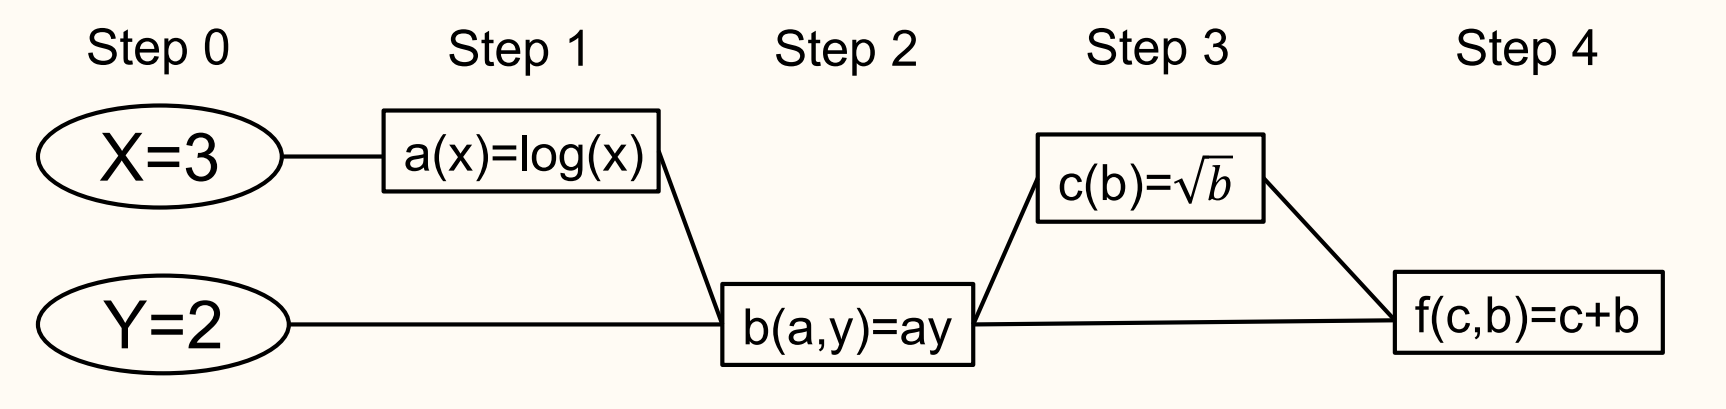
\includegraphics[width=1.0\textwidth]{.././assets/6.11.png}
    \end{figure}

    \begin{itemize}
        \item
        Step 0 :

        $$
        \begin{gathered}
        x=3, y=2 \\
        \frac{\partial x}{\partial x}=1, \frac{\partial x}{\partial y}=0, \frac{\partial y}{\partial x}=0, \frac{\partial y}{\partial y}=1
        \end{gathered}
        $$
        \item
        Step 1 :

        $$
        \begin{gathered}
        a=\log x=\log 3 \\
        \frac{\partial a}{\partial x}=\frac{1}{x} \cdot \frac{\partial x}{\partial x}=\frac{1}{3}, \frac{\partial a}{\partial y}=0
        \end{gathered}
        $$
        \item
        Step 2 :

        $$
        \begin{gathered}
        b=y a=2 \log 3 \\
        \frac{\partial b}{\partial x}=\frac{\partial y}{\partial x} a+y \frac{\partial a}{\partial x}=\frac{2}{3}, \frac{\partial b}{\partial y}=\frac{\partial y}{\partial y} a+y \frac{\partial a}{\partial y}=a=\log 3
        \end{gathered}
        $$
        \item
        Step 3 :

        $$
        \begin{gathered}
        c=\sqrt{b}=\sqrt{2 \log 3} \\
        \frac{\partial c}{\partial x}=\frac{1}{2 \sqrt{b}} \frac{\partial b}{\partial x}=\frac{1}{3 \sqrt{2 \log 3}}, \frac{\partial c}{\partial y}=\frac{1}{\sqrt{b}} \frac{\partial b}{\partial y}=\frac{1}{2} \sqrt{\frac{\log 3}{2}}
        \end{gathered}
        $$
        \item
        Step 4 :

        $$
        \begin{gathered}
        f=c+b=\sqrt{2 \log 3}+2 \log 3 \\
        \frac{\partial f}{\partial x}=\frac{\partial c}{\partial x}+\frac{\partial b}{\partial x}=\frac{1}{3}\left(2+\frac{1}{3 \sqrt{2 \log 3}}\right), \frac{\partial f}{\partial y}=\frac{\partial c}{\partial y}+\frac{\partial b}{\partial y}=\frac{1}{2} \sqrt{\frac{\log 3}{2}}+\log 3
        \end{gathered}
        $$
    \end{itemize}
\end{example}

\begin{definition}[6.42][Backprop on Computation Graph]
    To perform backprop, use

    $$
    \frac{\partial y_{L}}{\partial y_{i}}=\sum_{\ell: i \rightarrow \ell} \frac{\partial y_{L}}{\partial y_{\ell}} \frac{\partial f_{\ell}}{\partial y_{i}}
    $$

    to sequentially compute $\frac{\partial y_{L}}{\partial y_{L}}, \frac{\partial y_{L}}{\partial y_{L-1}}, \ldots, \frac{\partial y_{L}}{\partial y_{1}}$.\\\\ 

    \begin{verbatim}
    # Use 1-based indexing
    # y[1],...,y[L] already computed
    g[:] = 0 // .zero_grad()
    g[L] = 1 // dy[L]/dy[L]=1
    for l = L,...,2
        for i such that (i->l)
            g[i] += g[l]*f[l].grad(i)
        end
    end
    \end{verbatim}
\end{definition}

\begin{example}[6.43][Reverse-mode Autodiff (Backprop)]
    Consider $f(x, y)=y \log x+\sqrt{y \log x}$. Evaluate $f$ with the computation graph:

    \begin{figure}[H]
        \centering
        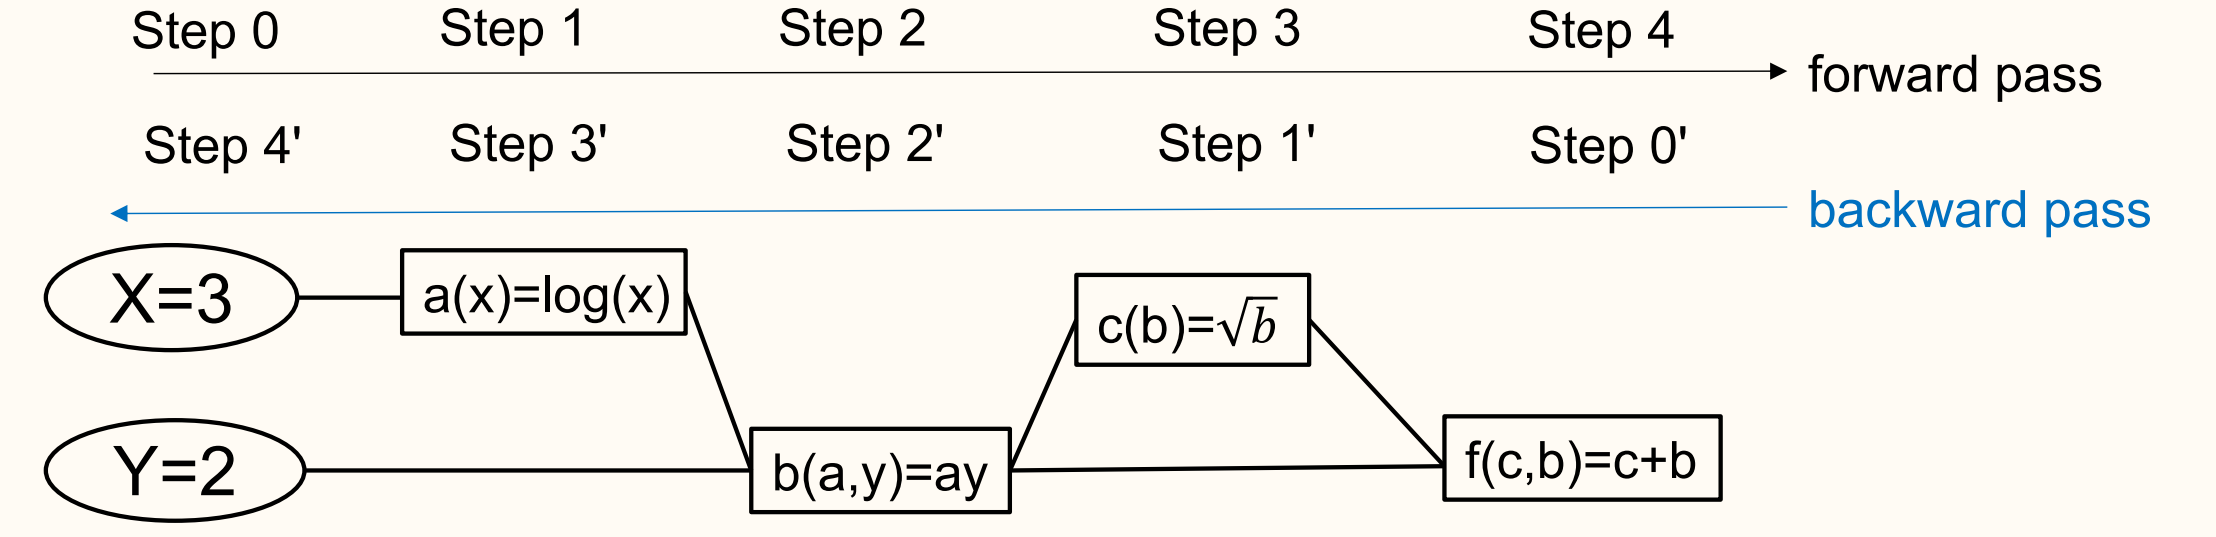
\includegraphics[width=1.0\textwidth]{.././assets/6.12.png}
    \end{figure}

    \begin{itemize}
        \item
        Step 0 :

        $$
        x=3, y=2
        $$
        \item
        Step 1 :

        $$
        a=\log 3
        $$
        \item
        Step 2 :

        $$
        b=2 \log 3
        $$
        \item
        Step 3 :

        $$
        c=\sqrt{2 \log 3}
        $$
        \item
        Step 4 :

        $$
        f=\sqrt{2 \log 3}+2 \log 3
        $$
    \end{itemize}

    \par\noindent\textcolor{gray}{\hdashrule{\textwidth}{0.4pt}{1pt 2pt}}

    \begin{itemize}
        \item
        Step 0' :

        $$
        \frac{\partial f}{\partial f}=1
        $$
        \item
        Step 1' :

        $$
        \frac{\partial f}{\partial c}=\frac{\partial f}{\partial f} \frac{\partial f}{\partial c}=\frac{\partial f}{\partial f} 1=1
        $$
        \item
        Step 2' :

        $$
        \frac{\partial f}{\partial b}=\frac{\partial f}{\partial c} \frac{\partial c}{\partial b}+\frac{\partial f}{\partial f} \frac{\partial f}{\partial c}=\frac{1}{2 \sqrt{b}} 1+1=\frac{1}{2 \sqrt{2 \log 3}}+1
        $$
        \item
        Step 3' :

        $$
        \frac{\partial f}{\partial a}=\frac{\partial f}{\partial b} \frac{\partial b}{\partial a}=\frac{\partial f}{\partial b} y=2+\frac{1}{\sqrt{2 \log 3}}
        $$
        \item
        Step 4' :

        $$
        \begin{gathered}
        \frac{\partial f}{\partial x}=\frac{\partial f}{\partial a} \frac{\partial a}{\partial x}=\frac{\partial f}{\partial a} \frac{1}{x}=\frac{1}{3}\left(2+\frac{1}{\sqrt{2 \log 3}}\right) \\
        \frac{\partial f}{\partial y}=\frac{\partial f}{\partial b} \frac{\partial b}{\partial y}=\frac{\partial f}{\partial b} a=\frac{1}{2} \sqrt{\frac{\log 3}{2}}+\log 3
        \end{gathered}
        $$
    \end{itemize}
\end{example}

\begin{concept}[6.44][Backprop in Pytorch]
    \begin{figure}[H]
        \centering
        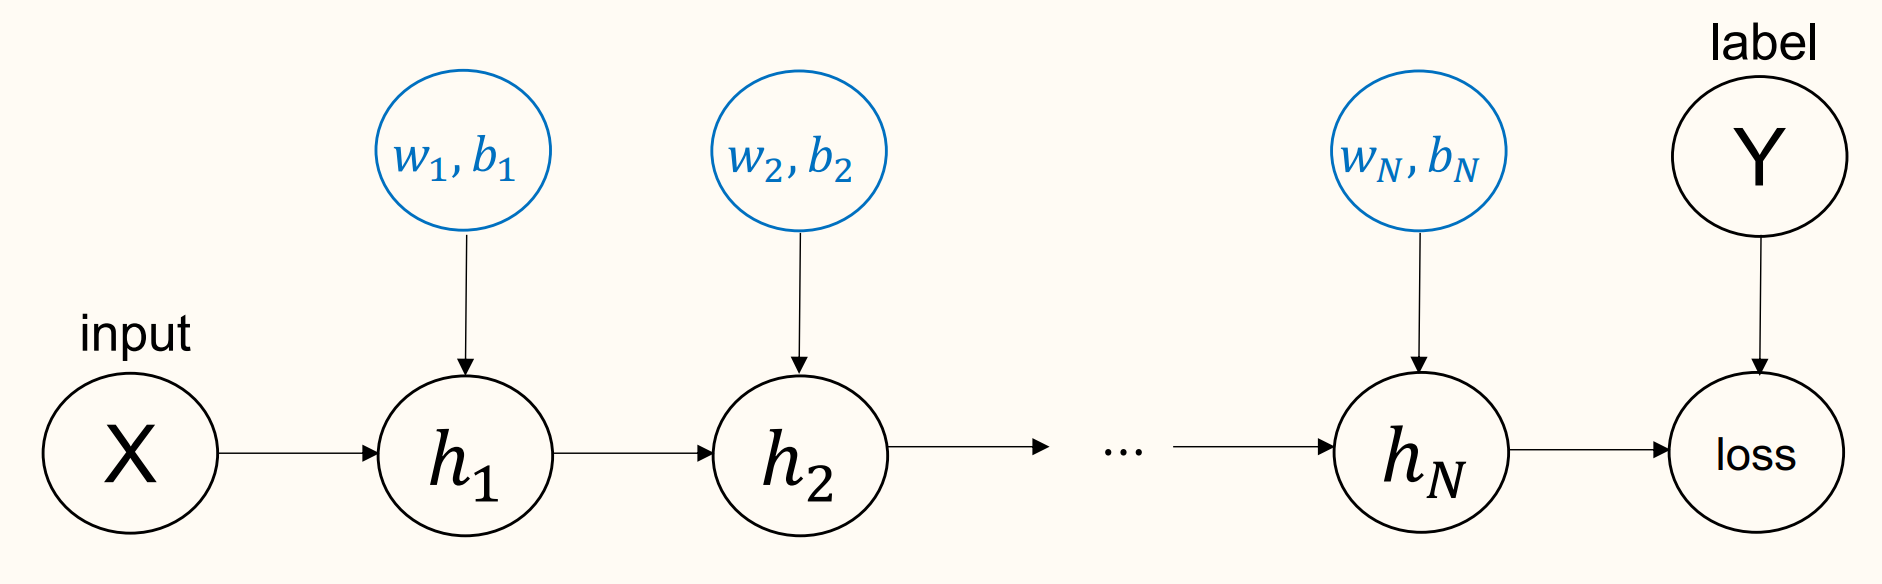
\includegraphics[width=1.0\textwidth]{.././assets/6.13.png}
    \end{figure}

    In NN training, parameters (shown blue in the image) and fixed inputs are distinguished.
    In PyTorch, you (1) clear the existing gradient with \verb|.zero_grad()|
    (2) forward-evaluate the loss function by providing the input and label and
    (3) perform backprop with \verb|.backward()|.

    The forward pass stores the intermediate neuron values so that they can later be used in backprop. In the test loop, however, we don't compute gradients so the intermediate neuron values are unnecessary.
    The \verb|torch.no_grad()| context manager allows intermediate node values to discarded or not be stored.
    This saves memory and can accelerate the test loop.
\end{concept}

\section{Batch Normalization}

\begin{concept}[6.45][Idea of Batch Normalization]
    The first step of many data processing algorithms is often to normalize data to have zero mean and unit variance.

    \begin{itemize}
        \item Step 1. Compute $\hat{\mu}=\frac{1}{N} \sum_{i=1}^{N} X_{i}, \widehat{\sigma^{2}}=\frac{1}{N} \sum_{i=1}^{N}\left(X_{i}-\hat{\mu}\right)^{2}$
    \end{itemize}

    $$
    \hat{X}_{i}=\frac{X_{i}-\widehat{\mu}}{\sqrt{\sigma^{2}}+\varepsilon}
    $$

    \begin{itemize}
        \item Step 2. Run method with data $\hat{X}_{1}, \ldots, \hat{X}_{N}$
    \end{itemize}

    \textbf{Batch normalization (BN)} (sort of) enforces this normalization layer-by-layer. BN is an indispensable tool for training very deep neural networks. Theoretical justification is weak.

    (S. Ioffe and C. Szegedy, Batch normalization: Accelerating deep network training by reducing internal covariate shift, ICML, 2015.)
\end{concept}

\begin{definition}[6.46][BN for Linear Layers]
    Underlying assumption: Each element of the batch is an IID sample.

    Input: $X$, $\text{shape}(X) = \text{(batch size)} \times \text{(\# entries)}$

    Output: $\mathrm{BN}_{\beta, \gamma}(X)$, $\text{shape} \left(\mathrm{BN}_{\beta, \gamma}(X)\right)=\operatorname{shape}(X)$

    $\mathrm{BN}_{\beta, \gamma}$ for linear layers acts independently over neurons.

    $$
    \begin{gathered}
    \hat{\mu}[:]=\frac{1}{B} \sum_{b=1}^{B} X[b,:]\\
    \hat{\sigma}^{2}[:]=\frac{1}{B} \sum_{b=1}^{B}(X[b,:]-\hat{\mu}[:])^{2} \\
    \mathrm{BN}_{\gamma, \beta}(X)[b,:]=\gamma[:] \frac{X[b,:]-\hat{\mu}[:]}{\sqrt{\hat{\sigma}^{2}[:]+\varepsilon}}+\beta[:] \quad b=1, \ldots, B
    \end{gathered}
    $$

    where operations are elementwise. BN normalizes each output neuron. The mean and variance are explicitly controlled through learned parameters $\beta$ and $\gamma$. In Pytorch, \verb|nn.BatchNorm1d|.
\end{definition}

\begin{definition}[6.47][BN for Convolutional Layers]
    Underlying assumption: Each element of the batch, horizontal pixel, and vertical pixel is an IID sample.

    Input: $X$, $\text{shape}(X) =\\\text{(batch size)} \times \text{(channels)} \times \text{(vertical dim)} \times \text{(horizontal dim)}$

    Output: $\mathrm{BN}_{\beta, \gamma}(X)$, $\text{shape} \left(\mathrm{BN}_{\beta, \gamma}(X)\right)=\operatorname{shape}(X)$

    $\mathrm{BN}_{\beta, \gamma}$ for conv. layers acts independently over channels.

    $$
    \begin{gathered}
    \hat{\mu}[:]=\frac{1}{B P Q} \sum_{b=1}^{B} \sum_{i=1}^{P} \sum_{j=1}^{Q} X[b,:, i, j] \\
    \hat{\sigma}^{2}[:]=\frac{1}{B P Q} \sum_{b=1}^{B} \sum_{i=1}^{P} \sum_{j=1}^{Q}(X[b,:, i, j]-\hat{\mu}[:])^{2} \\
    \operatorname{BN}_{\gamma, \beta}(X)[b,:, i, j]=\gamma[:] \frac{X[b,:, i, j]-\hat{\mu}[:]}{\sqrt{\hat{\sigma}^{2}[:]+\varepsilon}}+\beta[:] \quad \begin{array}{l}
    b=1, \ldots, B \\
    i=1, \ldots, P \\
    j=1, \ldots, Q
    \end{array}
    \end{gathered}
    $$

    BN normalizes over each convolutional filter. The mean and variance are explicitly controlled through learned parameters $\beta$ and $\gamma$. In Pytorch, \verb|nn.BatchNorm2d|.
\end{definition}

\begin{definition}[6.48][BN during Testing]
    $\hat{\mu}$ and $\hat{\sigma}$ are estimated from batches during training. During testing, we don't update the NN, and we may only have a single input (so no batch).

    There are 2 strategies for computing final values of $\hat{\mu}$ and $\hat{\sigma}$ :

    \begin{enumerate}
        \item After training, fix all parameters and evaluate NN on full training set to compute $\hat{\mu}$ and $\hat{\sigma}$ layer-by-layer. Store this computed value. (Computation of $\hat{\mu}$ and $\hat{\sigma}$ must be done sequentially layer-by-layer. Why?)
        \item During training, compute running average of $\hat{\mu}$ and $\hat{\sigma}$. This is the default behavior of PyTorch.
    \end{enumerate}

    In PyTorch, use \verb|model.train()| and \verb|model.eval()| to switch BN behavior between training and testing.
\end{definition}

\begin{concept}[6.49][Efficiency of BN]
    BN does not change the representation power of NN ; since $\beta$ and $\gamma$ are trained, the output of each layer can have any mean and variance. However, controlling the mean and variance as explicit trainable parameters makes training easier.

    With BN, the choice of batch size becomes a more important hyperparameter to tune.

    BN is indispensable in practice. Training of VGGNet and GoogLeNet becomes much easier with BN. Training of ResNet requires BN.
\end{concept}

\begin{concept}[6.51][BN and Internal Covariate Shift]
    BN has insufficient theoretical justification.
    The original paper by loffe and Szegedy hypothesized that BN mitigates internal covariate shift (ICS), the shift in the mean and variance of the intermediate layer neurons throughout the training, and that this mitigation leads to improved training.

    $$
    \mathrm{BN} \Rightarrow(\text { reduced ICS }) \Rightarrow \text { (improved training })
    $$

    However, Santukar et al. demonstrated that when experimentally measured, BN does not mitigate ICS, but nevertheless improves the training.

    $$
    \mathrm{BN} \nRightarrow \text { (reduced ICS) }
    $$

    Nevertheless

    $$
    \mathrm{BN} \Rightarrow \text { (improved training performance) }
    $$

    Santukar et al. argues that

    $$
    \mathrm{BN} \Rightarrow \text { (smoother loss landscape) } \Rightarrow \text { (improved training performance) }
    $$

    While this claim is more evidence-based than that of loffe and Szegedy, it is still not conclusive. It is also unclear why BN makes the loss landscape smoother, and it is not clear whether the smoother loss landscape fully explains the improved training performance.

    This story is a cautionary tale: we should carefully distinguish between speculative hypotheses and evidence-based claims, even in a primarily empirical subject.

    (S. Ioffe and C. Szegedy, Batch normalization: Accelerating deep network training by reducing internal covariate shift, ICML, 2015.\\
    S. Santurkar, D. Tsipras, A. Ilyas, and A. Mądry, How does batch normalization help optimization?, NeurIPS, 2018.)
\end{concept}

\begin{concept}[6.50][BN has trainable parameters.]
    BN is usually not considered a trainable layer, much like pooling or dropout, and they are usually excluded when counting the "depth" of a NN. However, BN does have trainable parameters. Interestingly, if one randomly initializes a CNN, freezes all other parameters, and only train BN parameters, the performance is surprisingly good.

    \begin{figure}[H]
        \centering
        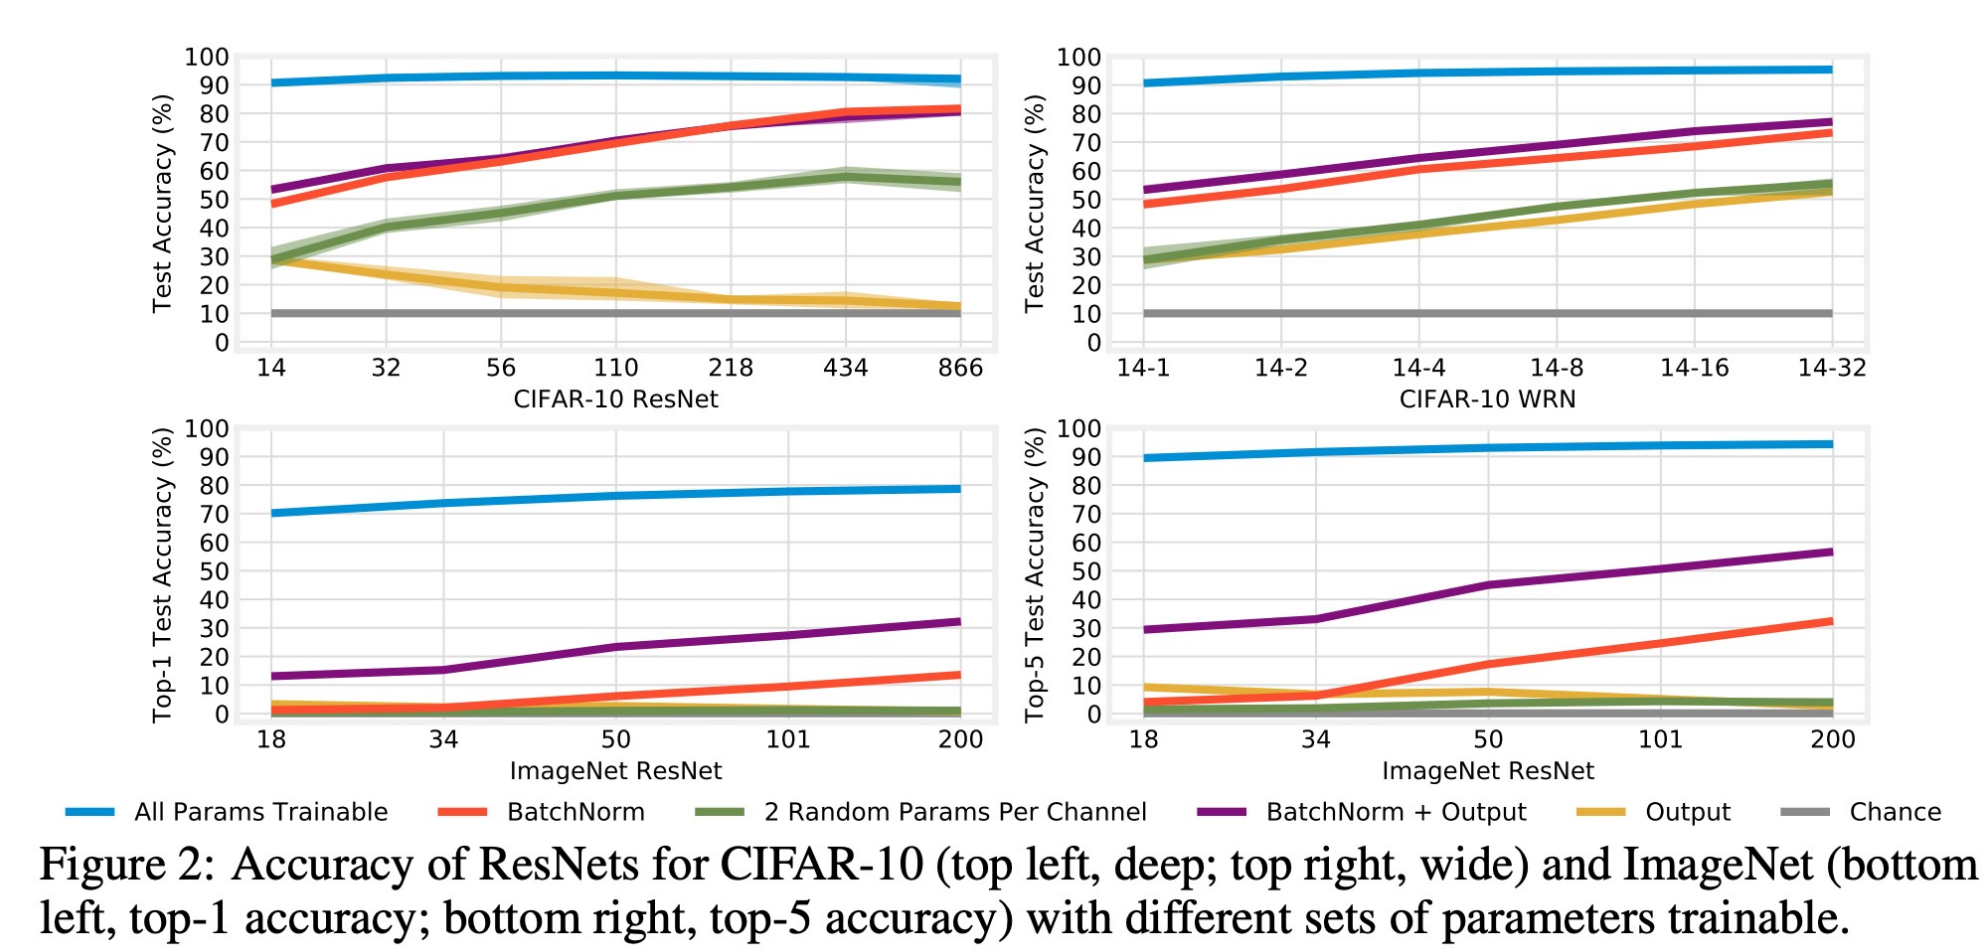
\includegraphics[width=0.75\textwidth]{.././assets/6.14.png}
    \end{figure}

    (J. Frankle, D. J. Schwab, and A. S. Morcos, Training BatchNorm and only BatchNorm: On the expressive power of random features in CNNs, NeurIPS SEDL Workshop, 2019.)
\end{concept}

\begin{concept}[6.51][Discussion of BN]
    BN seems to also act as a regularizer, and for some reason subsumes effect Dropout. (Using dropout together with BN seems to worsen performance.) Since BN has been popularized, Dropout is used less often.

    After training, functionality of BN can be absorbed into the previous layer when the previous layer is a linear layer or a conv layer.

    The use of batch norm makes the scaling of weight initialization less important irrelevant.

    Use \verb|bias=false| on layers preceding BN , since $\beta$ subsumes the bias.

    (X. Li, S. Chen, X. Hu and J. Yang, Understanding the disharmony between dropout and batch normalization by variance shift, CVPR, 2019.)
\end{concept}

\chapter{ImageNet Challenge}

\begin{definition}[7.1][ImageNet Dataset]
    \textbf{ImageNet} contains more 14 million hand-annotated images in more than 20,000 categories.
    Many classes, higher resolution, non-uniform image size, multiple objects per image.

    \begin{figure}[H]
        \centering
        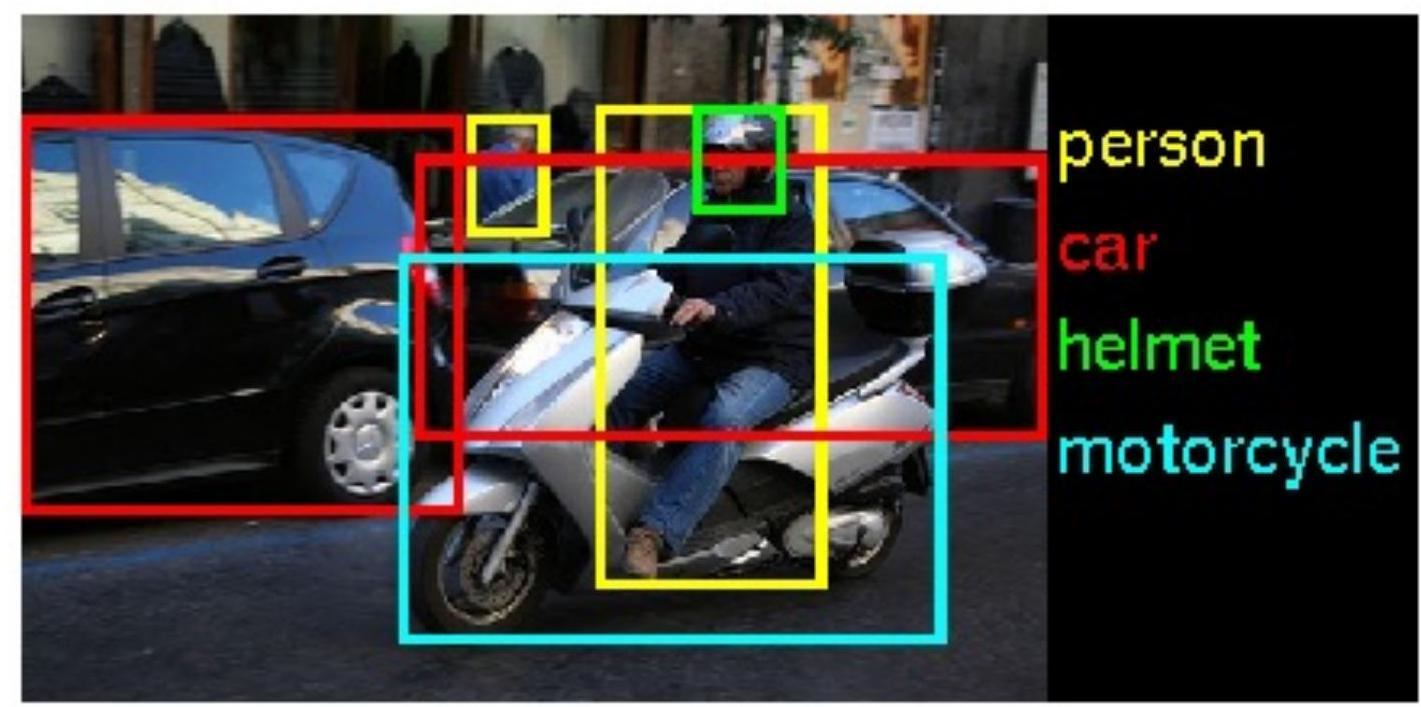
\includegraphics[width=0.6\textwidth]{.././assets/7.1.jpg}
    \end{figure}

    \par\noindent\textcolor{gray}{\hdashrule{\textwidth}{0.4pt}{1pt 2pt}}

    \textbf{History}

    \begin{itemize}
        \item Fei-Fei Li started the ImageNet project in 2006 with the goal of expanding and improving the data available for training Al algorithms.
        \item Images were annotated with Amazon Mechanical Turk.
        \item The ImageNet team first presented their dataset in the 2009 Conference on Computer Vision and Pattern Recognition (CVPR).
        \item From 2010 to 2017, the ImageNet project ran the ImageNet Large Scale Visual Recognition Challenge (ILSVRC).
        \item In the 2012 ILSVRC challenge, 150,000 images of 1000 classes were used.
        \item In 2017, 29 teams achieved above 95\% accuracy. The organizers deemed task complete and ended the ILSVRC competition.
    \end{itemize}

    \par\noindent\textcolor{gray}{\hdashrule{\textwidth}{0.4pt}{1pt 2pt}}

    \textbf{ImageNet-1k}

    Commonly referred to as "the ImageNet dataset". Also called ImageNet2012.
    However, ImageNet-1k is really a subset of full ImageNet dataset.
    ImageNet-1k has 150,000 images of 1000 roughly balanced classes.

    \begin{figure}[H]
        \centering
        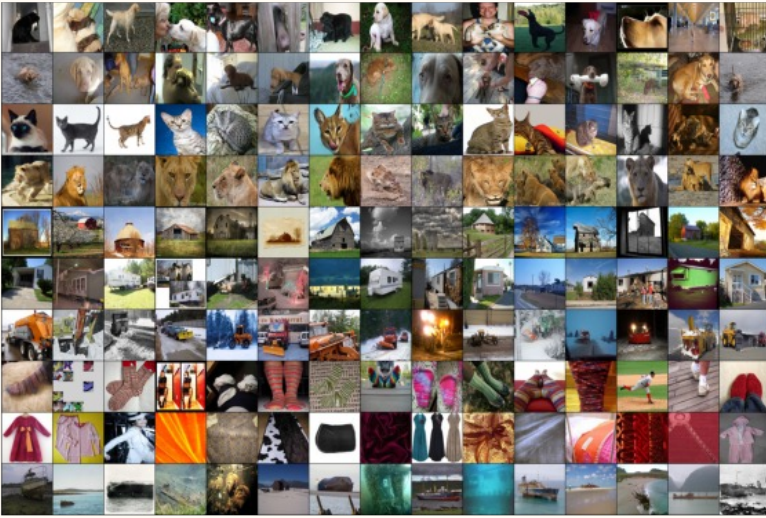
\includegraphics[width=0.8\textwidth]{.././assets/7.2.png}
    \end{figure}

    \par\noindent\textcolor{gray}{\hdashrule{\textwidth}{0.4pt}{1pt 2pt}}

    \textbf{Top-1 vs Top-5 Accuracy}

    Classifiers on ImageNet-1k are often assessed by their top-5 accuracy, which requires the 5 categories with the highest confidence to contain the label.
    In contrast, the top-1 accuracy simply measures whether the network's single prediction is the label.

    For example, AlexNet had a top-5 accuracy of 84.6% and a top-1 accuracy of 63.3%.
    Nowadays, accuracies of classifiers has improved, so the top 1 accuracy is becoming the more common metric.
\end{definition}

\section{LeNet}

\begin{definition}[7.2][LeNet5]
    \begin{figure}[H]
        \centering
        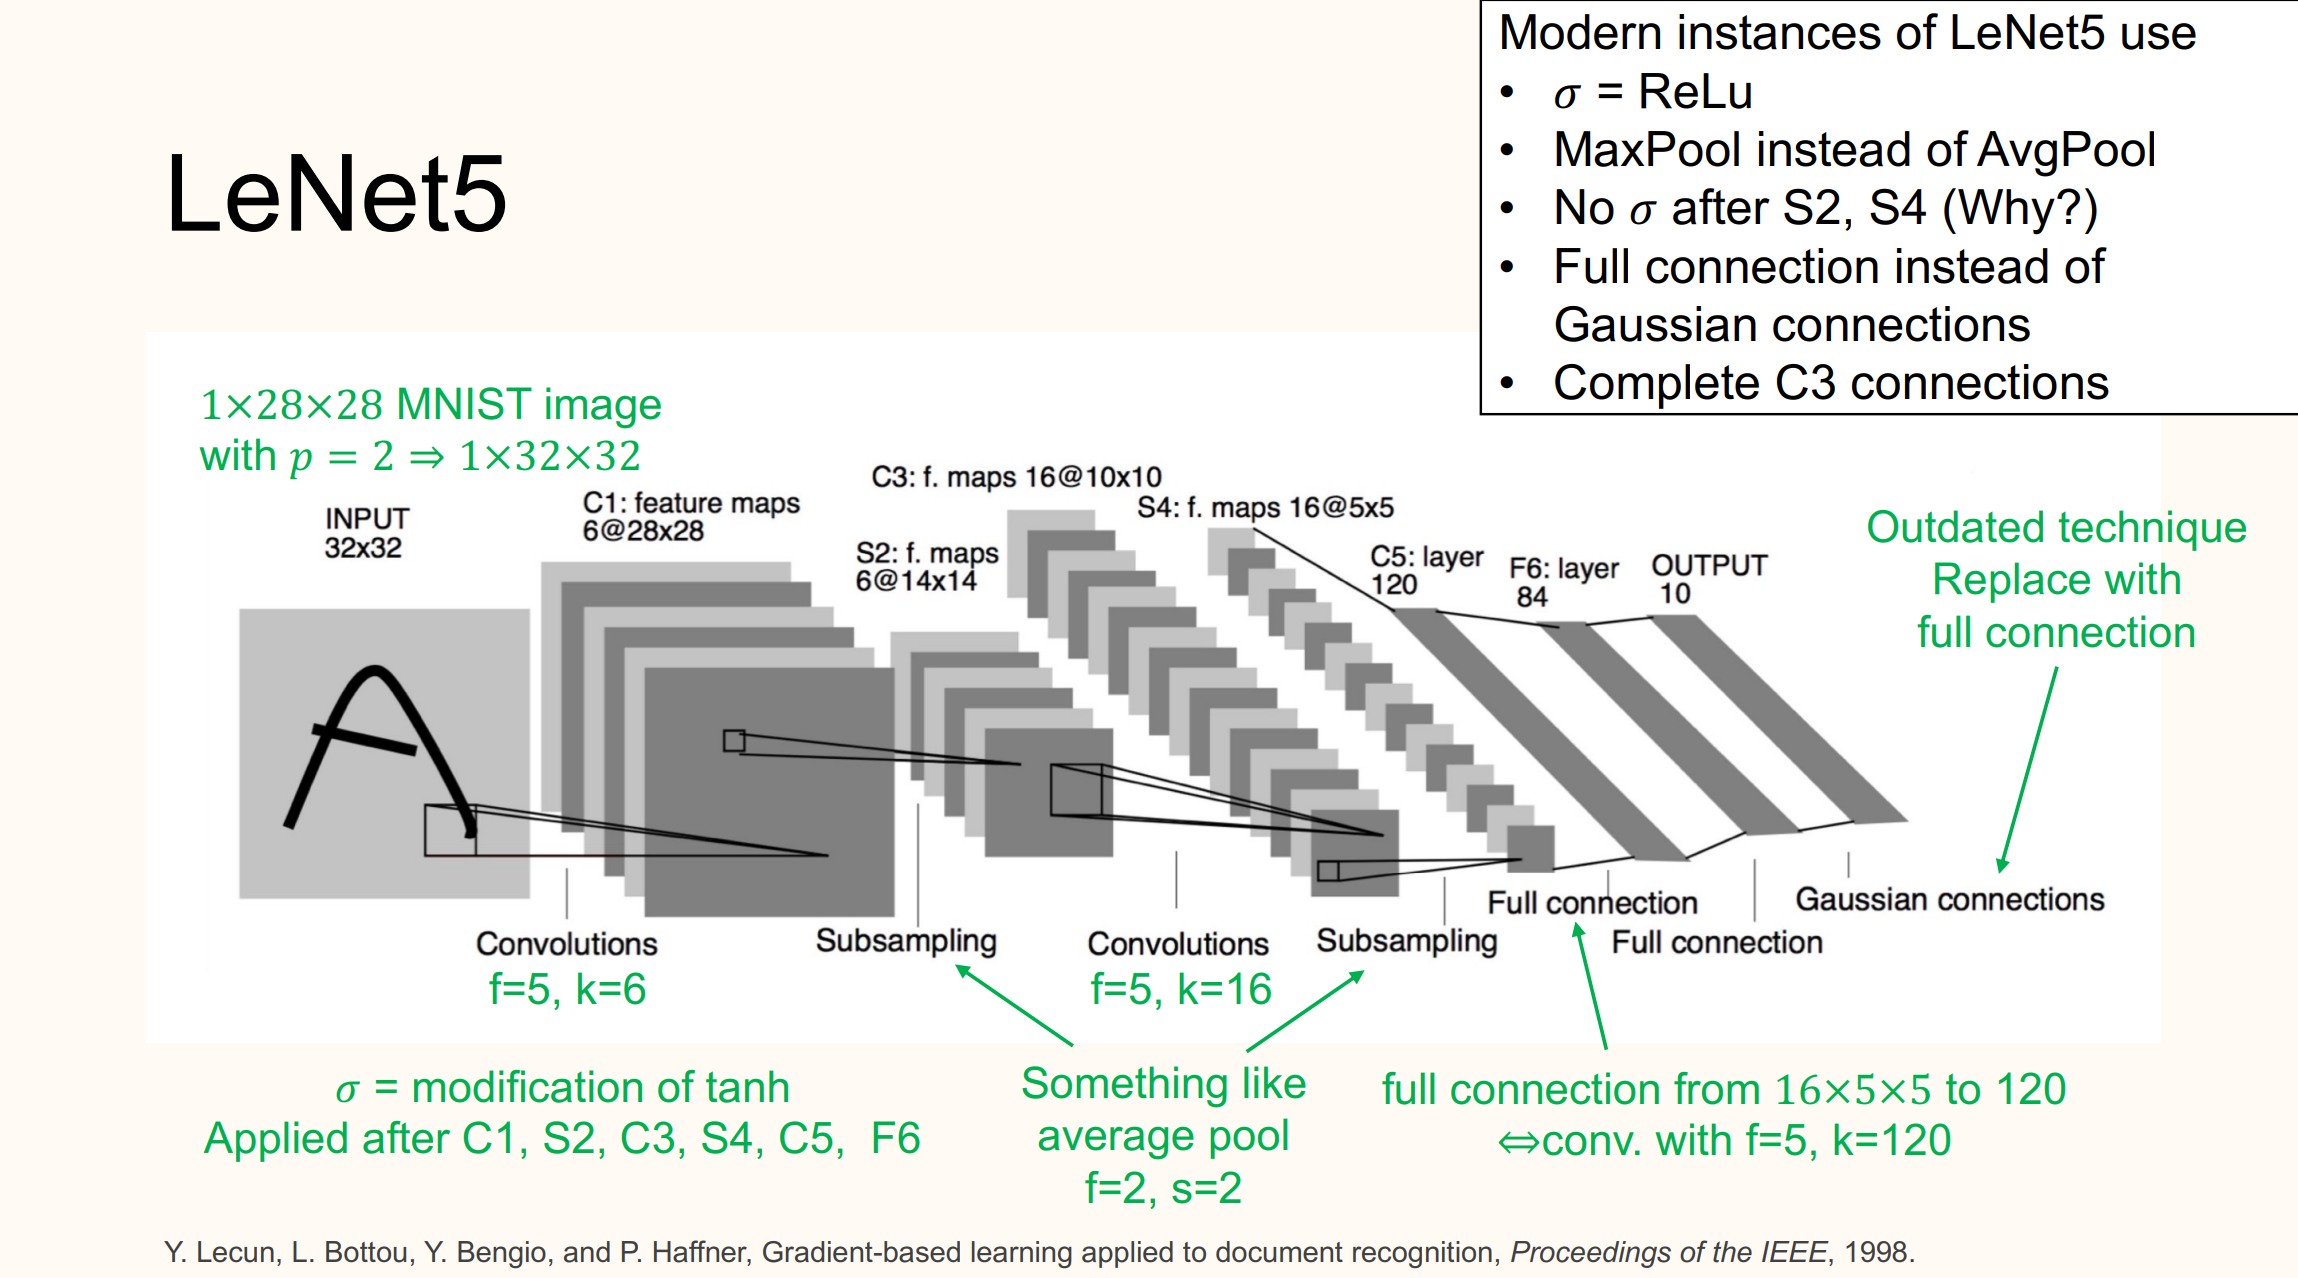
\includegraphics[width=1.0\textwidth]{.././assets/7.3.png}
    \end{figure}

    (Y. Lecun, L. Bottou, Y. Bengio, and P. Haffner, Gradient-based learning applied to document recognition, Proceedings of the IEEE, 1998.)
\end{definition}

\begin{concept}[7.3][Architectural Contribution]
    One of the earliest demonstration of using a deep CNN to learn a nontrivial task.

    Laid the foundation of the modern CNN architecture.
\end{concept}

\section{AlexNet}

\begin{definition}[7.4][AlexNet]
    Won the 2012 ImageNet challenge by a large margin: top-5 error rate $15.3 \%$ vs. $26.2 \%$ second place.

    Started the era of deep neural networks and their training via GPU computing.

    AlexNet was split into 2 as GPU memory was limited. (A single modern GPU can easily hold AlexNet.)

    \begin{figure}[H]
        \centering
        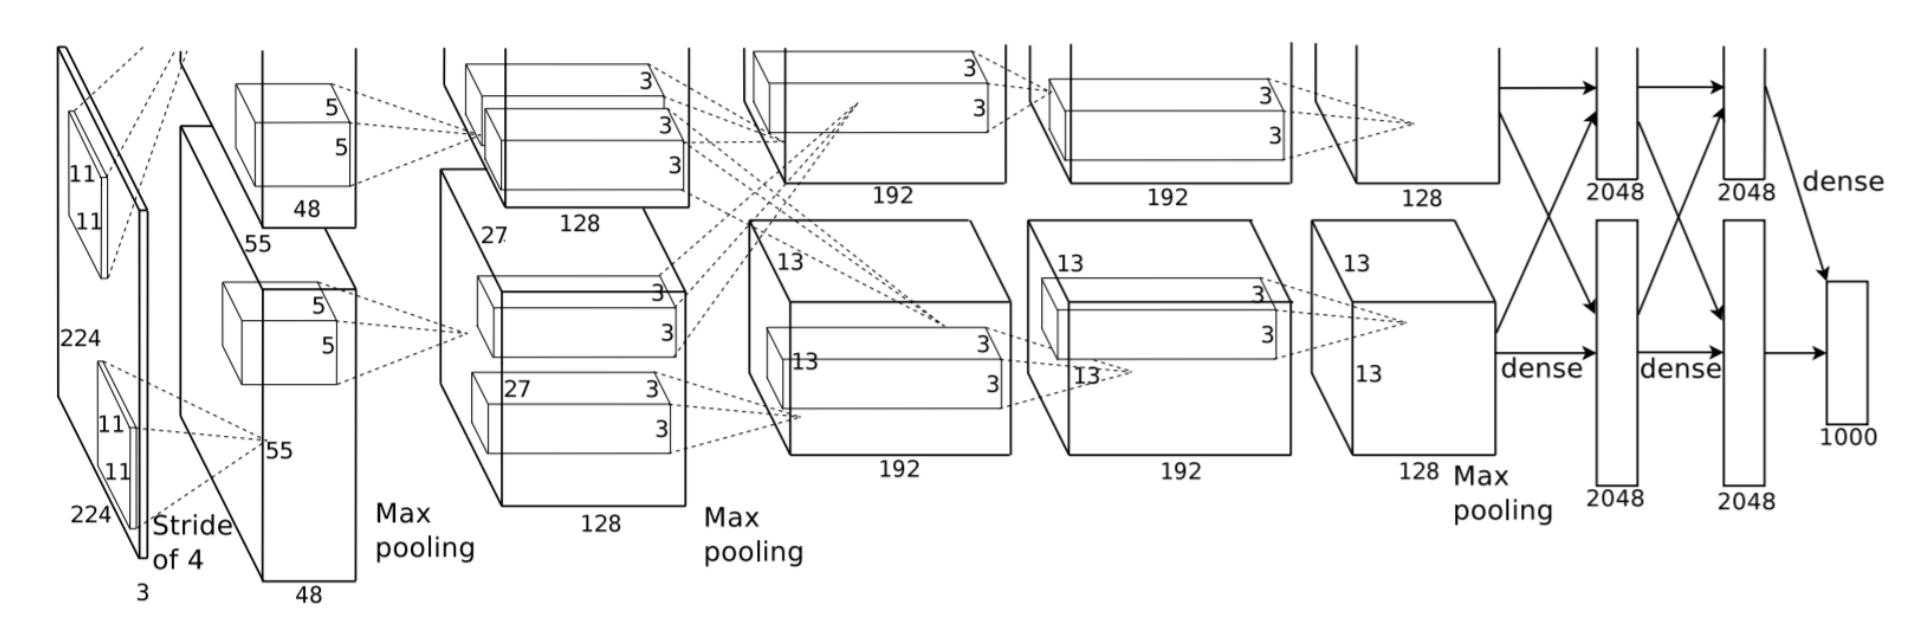
\includegraphics[width=1.0\textwidth]{.././assets/7.4.png}
    \end{figure}

    (A. Krizhevsky, I. Sutskever, and G. E. Hinton, ImageNet classification with deep convolutional neural networks, NeurIPS, 2012.)
\end{definition}

\begin{definition}[7.5][AlexNet for ImageNet]
    \begin{figure}[H]
        \centering
        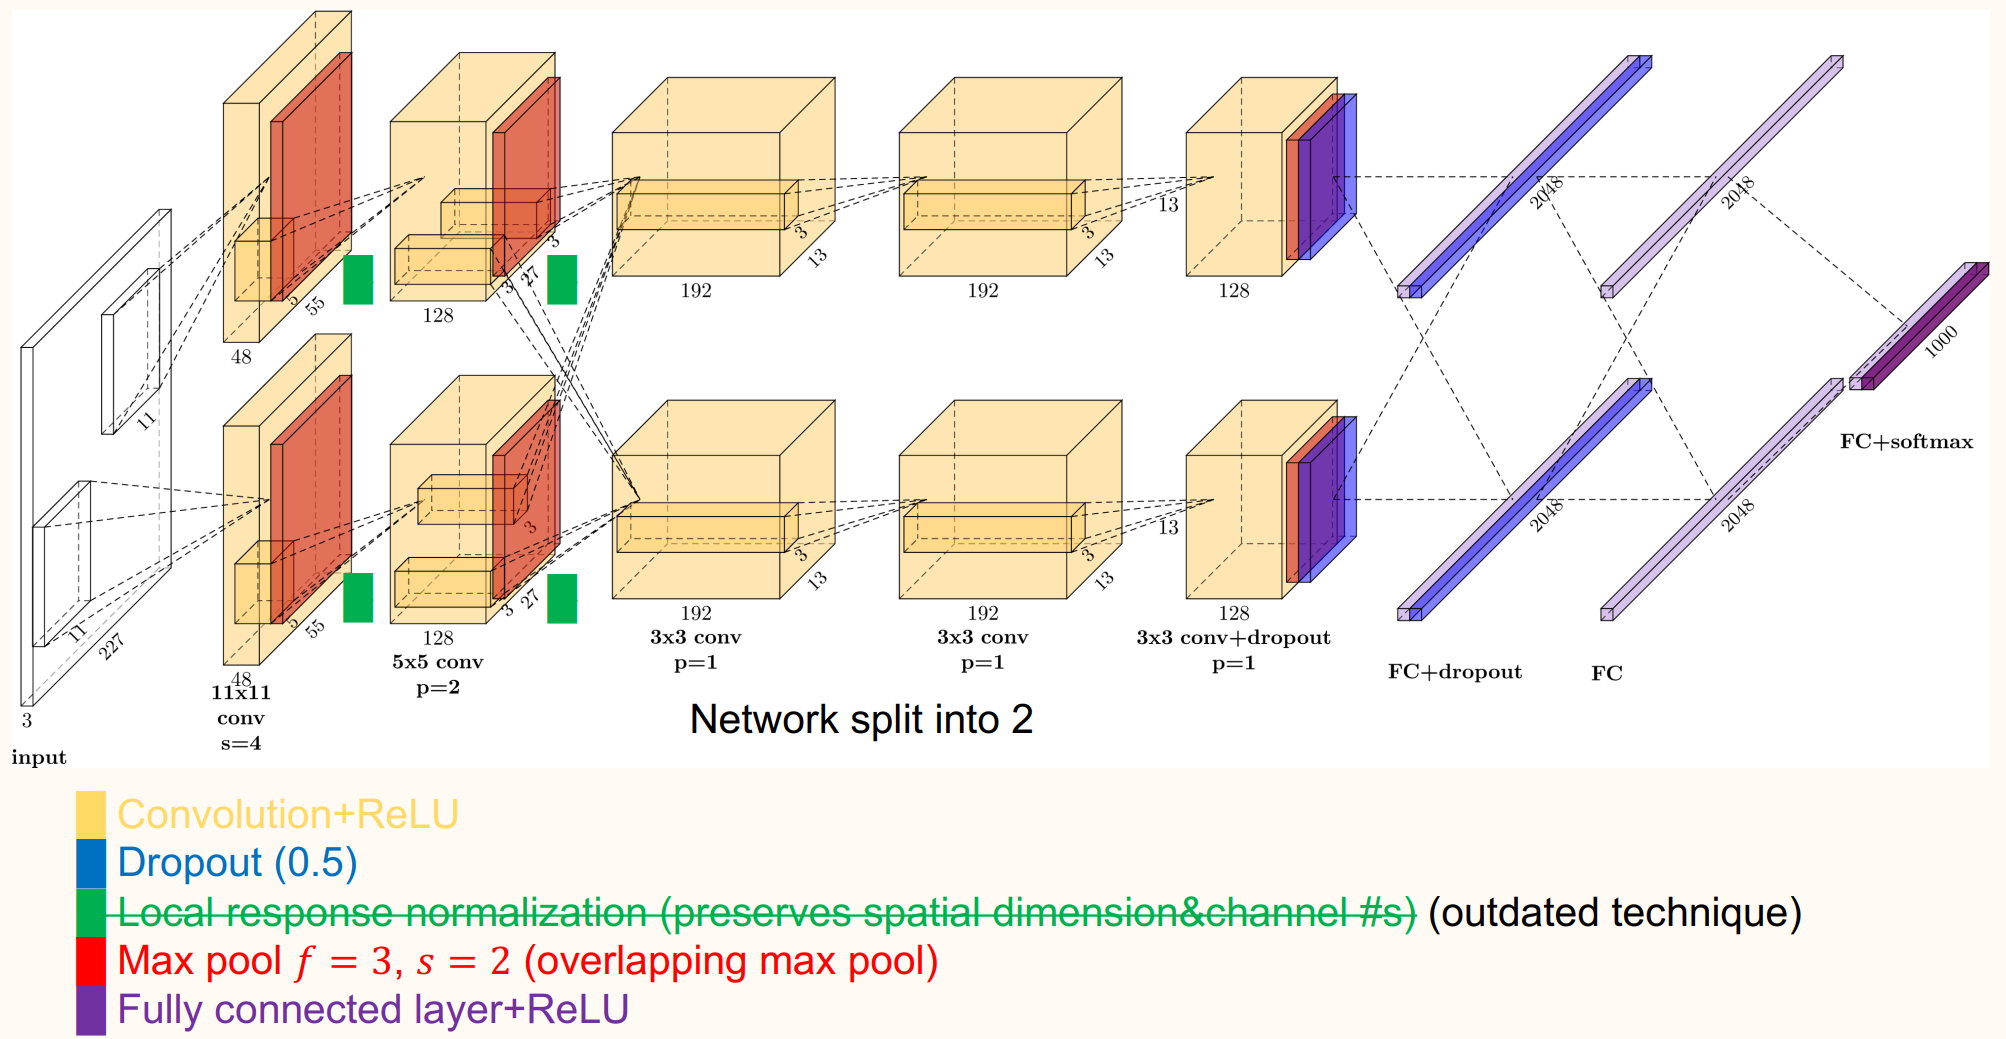
\includegraphics[width=1.0\textwidth]{.././assets/7.5.png}
    \end{figure}
\end{definition}

\begin{definition}[7.6][AlexNet for Cifar10]
    \begin{figure}[H]
        \centering
        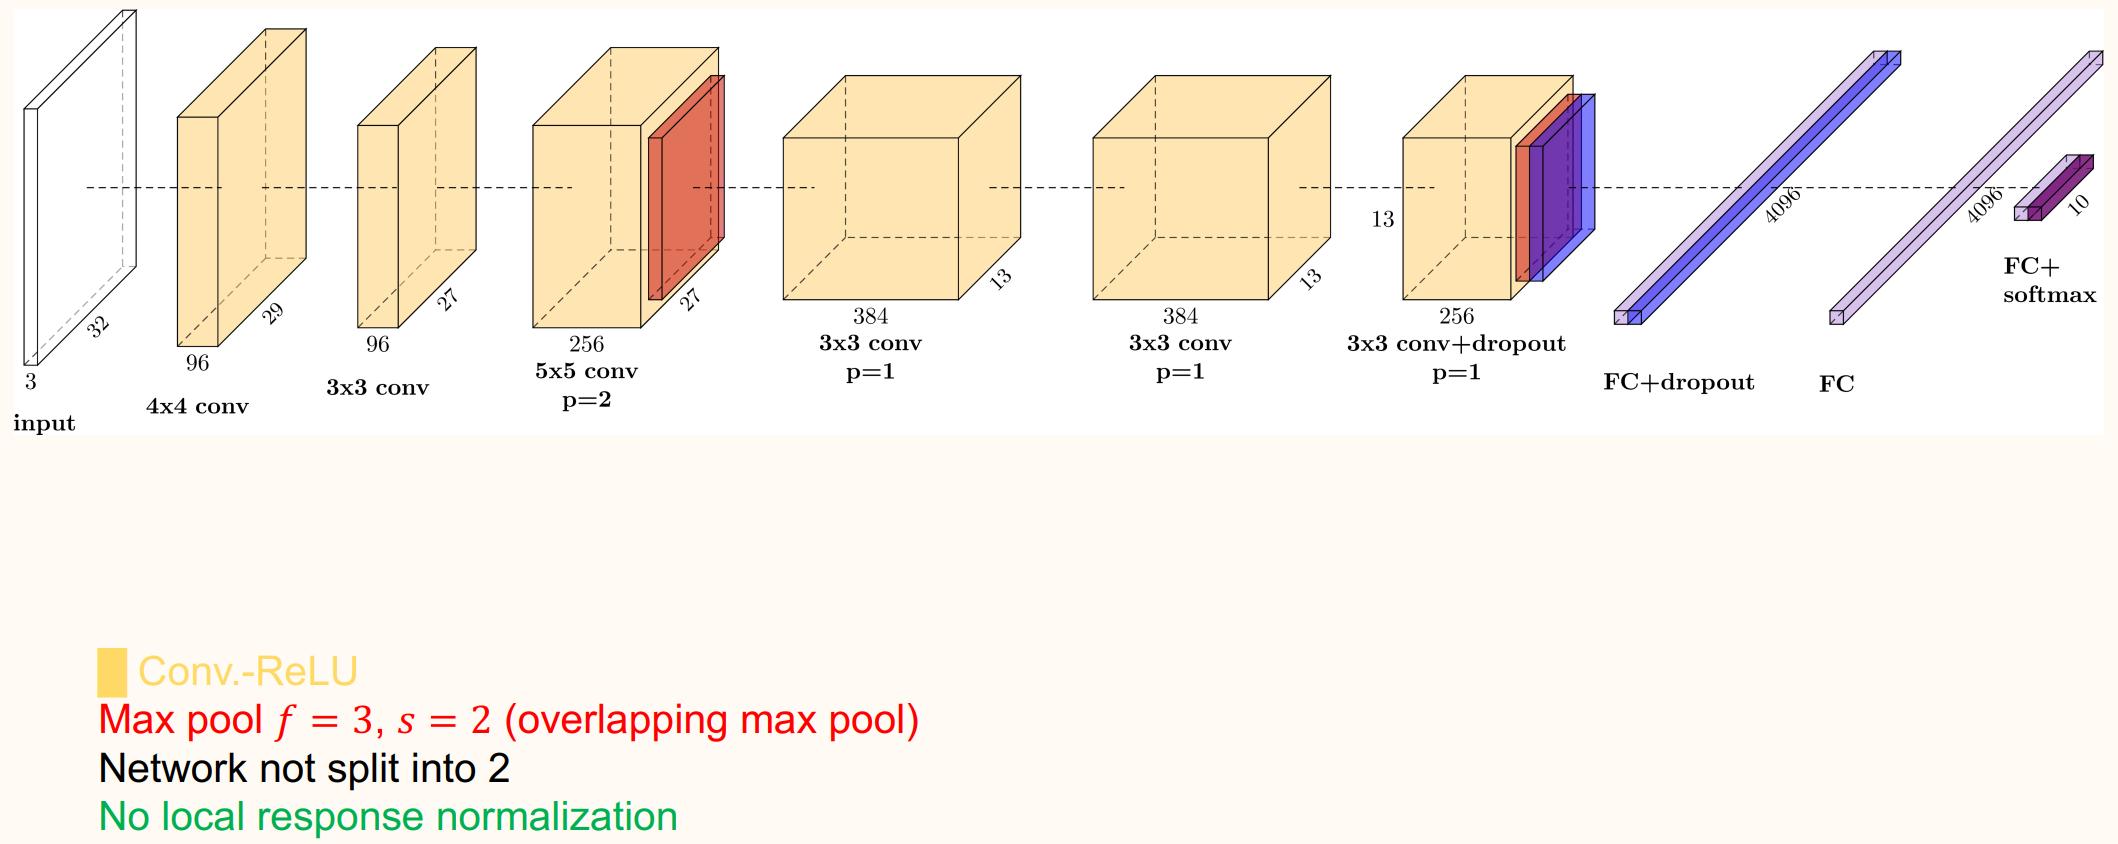
\includegraphics[width=1.0\textwidth]{.././assets/7.6.png}
    \end{figure}
\end{definition}

\begin{concept}[7.7][Architectural Contribution]
    A scaled-up version of LeNet.

    Demonstrated that deep CNNs can learn significantly complex tasks. (Some thought CNNs could only learn simple, toy tasks like MNIST.)

    Demonstrated GPU computing to be an essential component of deep learning.

    Demonstrated effectiveness of ReLU over sigmoid or tanh in deep CNNs for classification.
\end{concept}

\section{VGGNet}

\begin{definition}[7.8][VGGNet]
    \begin{figure}[H]
        \centering
        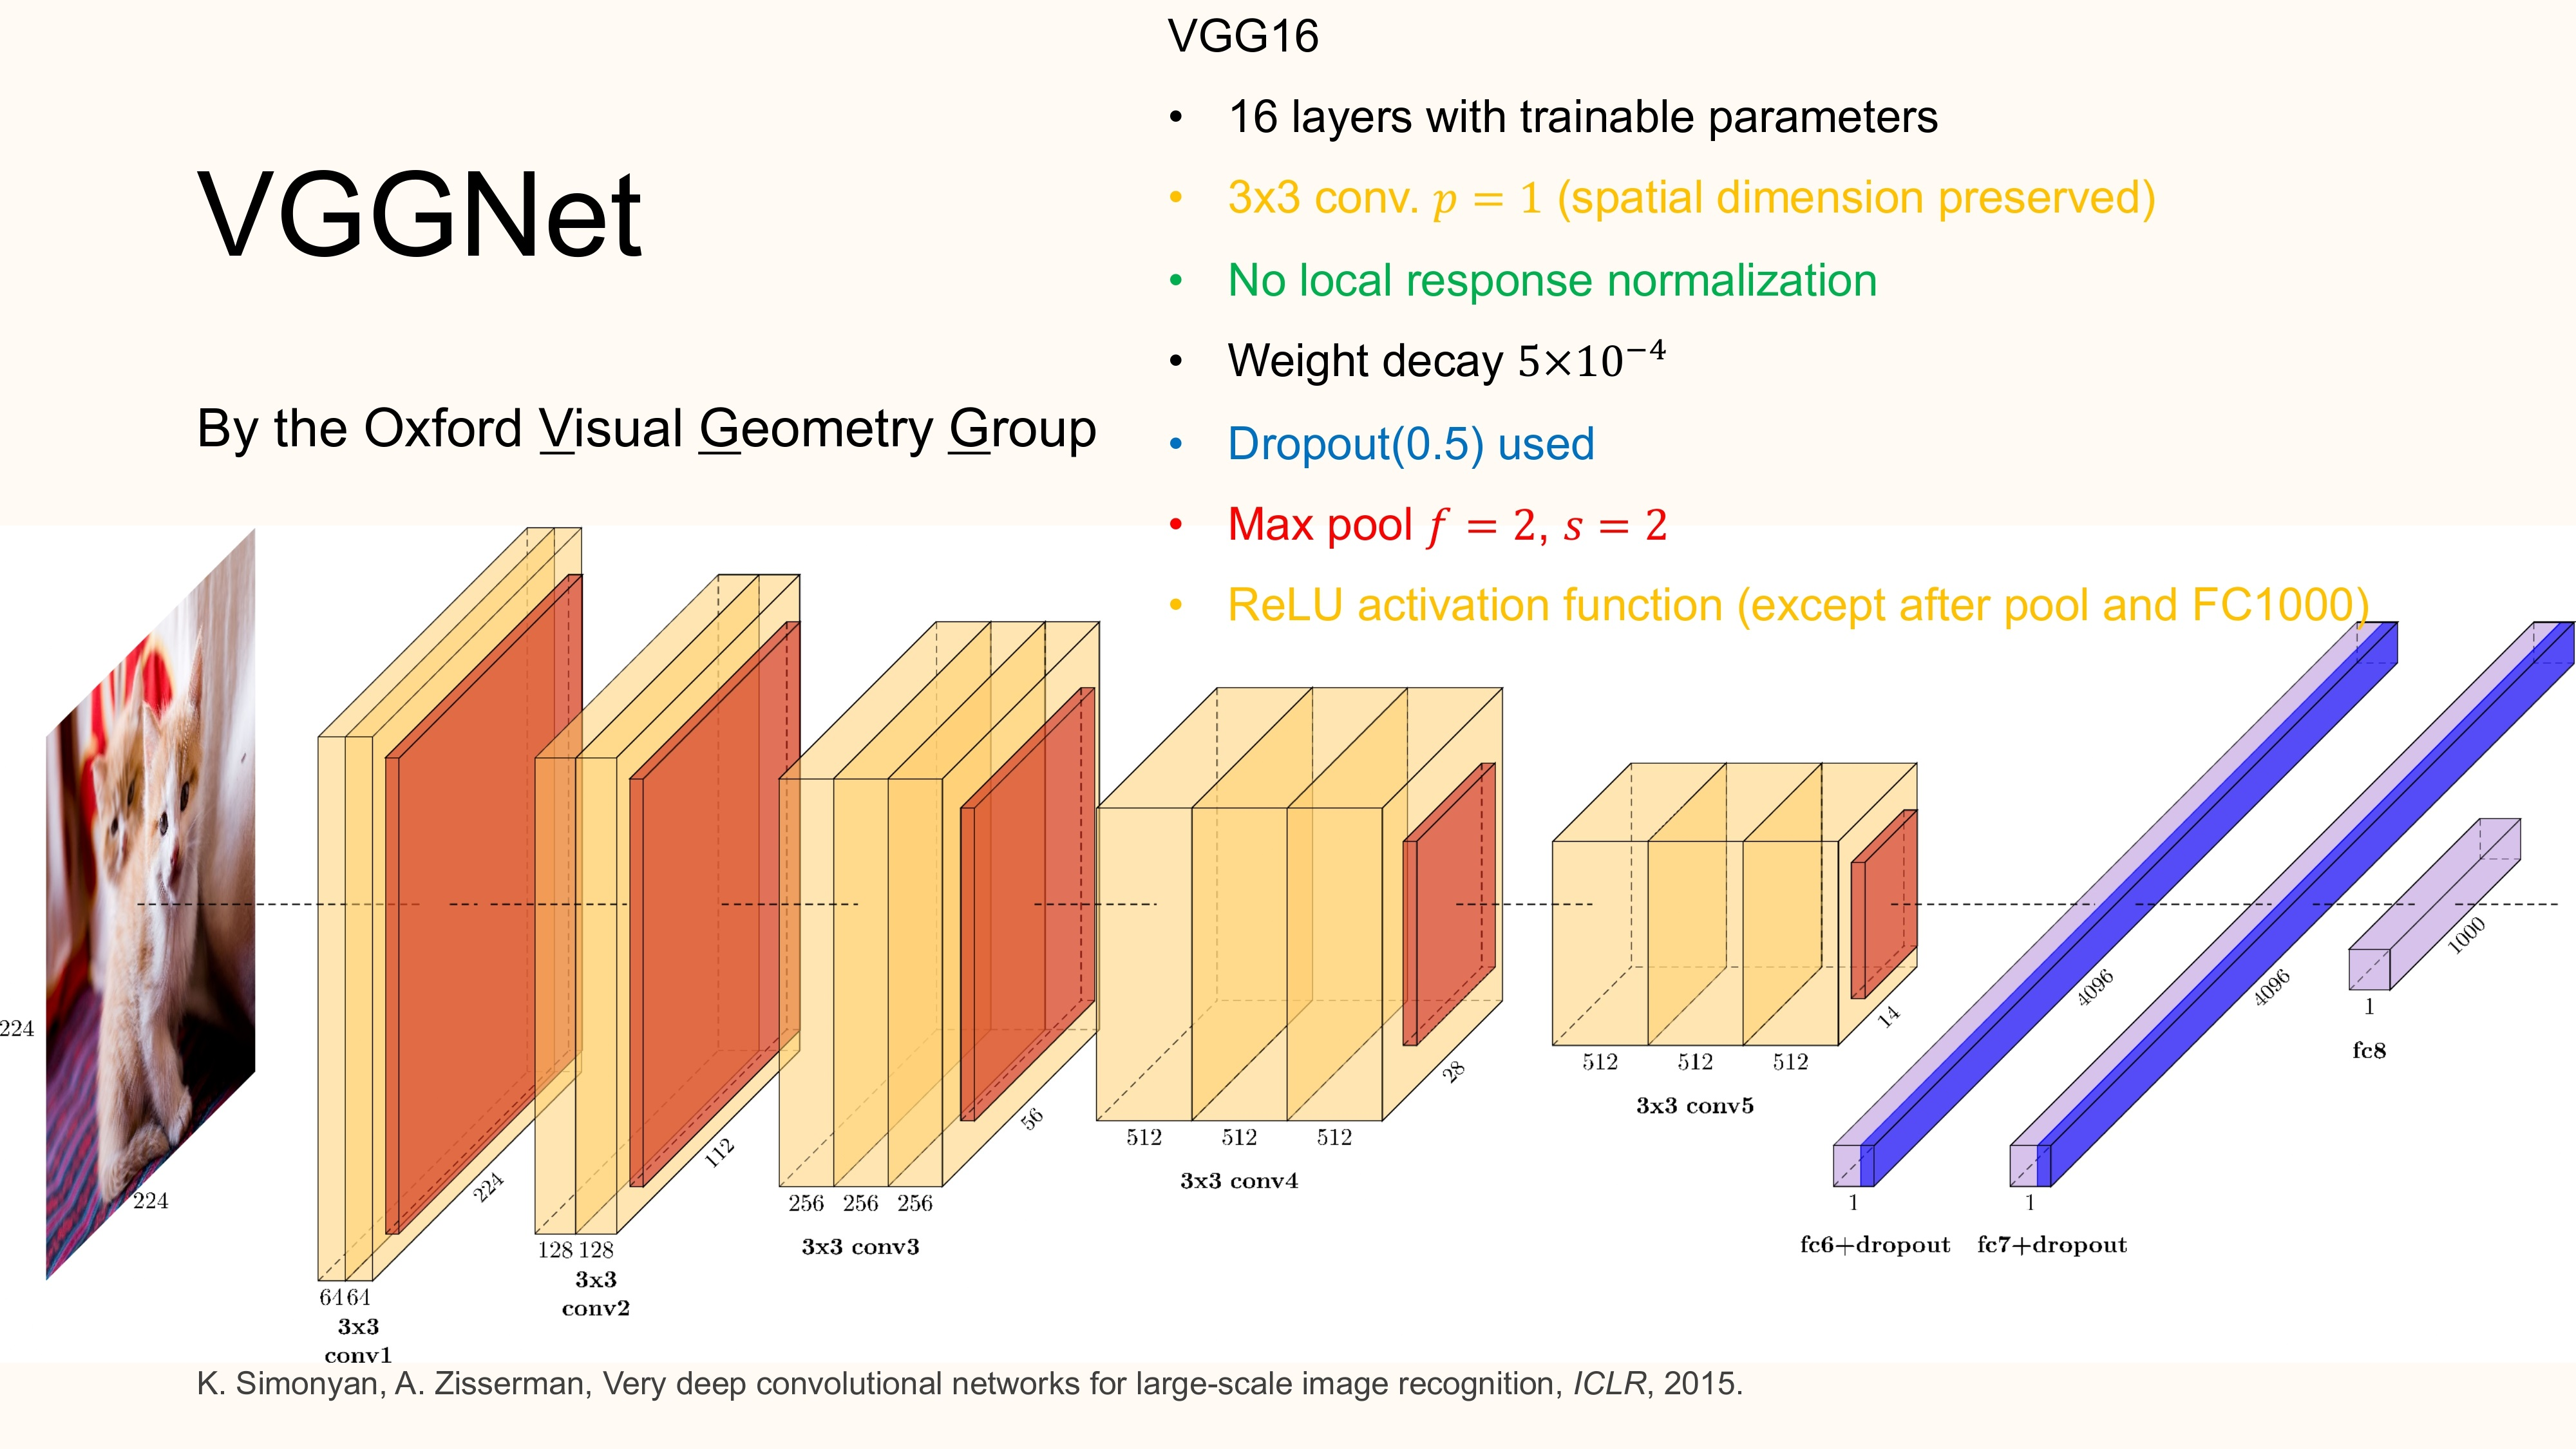
\includegraphics[width=1.0\textwidth]{.././assets/7.7.jpg}
    \end{figure}

    \begin{figure}[H]
        \centering
        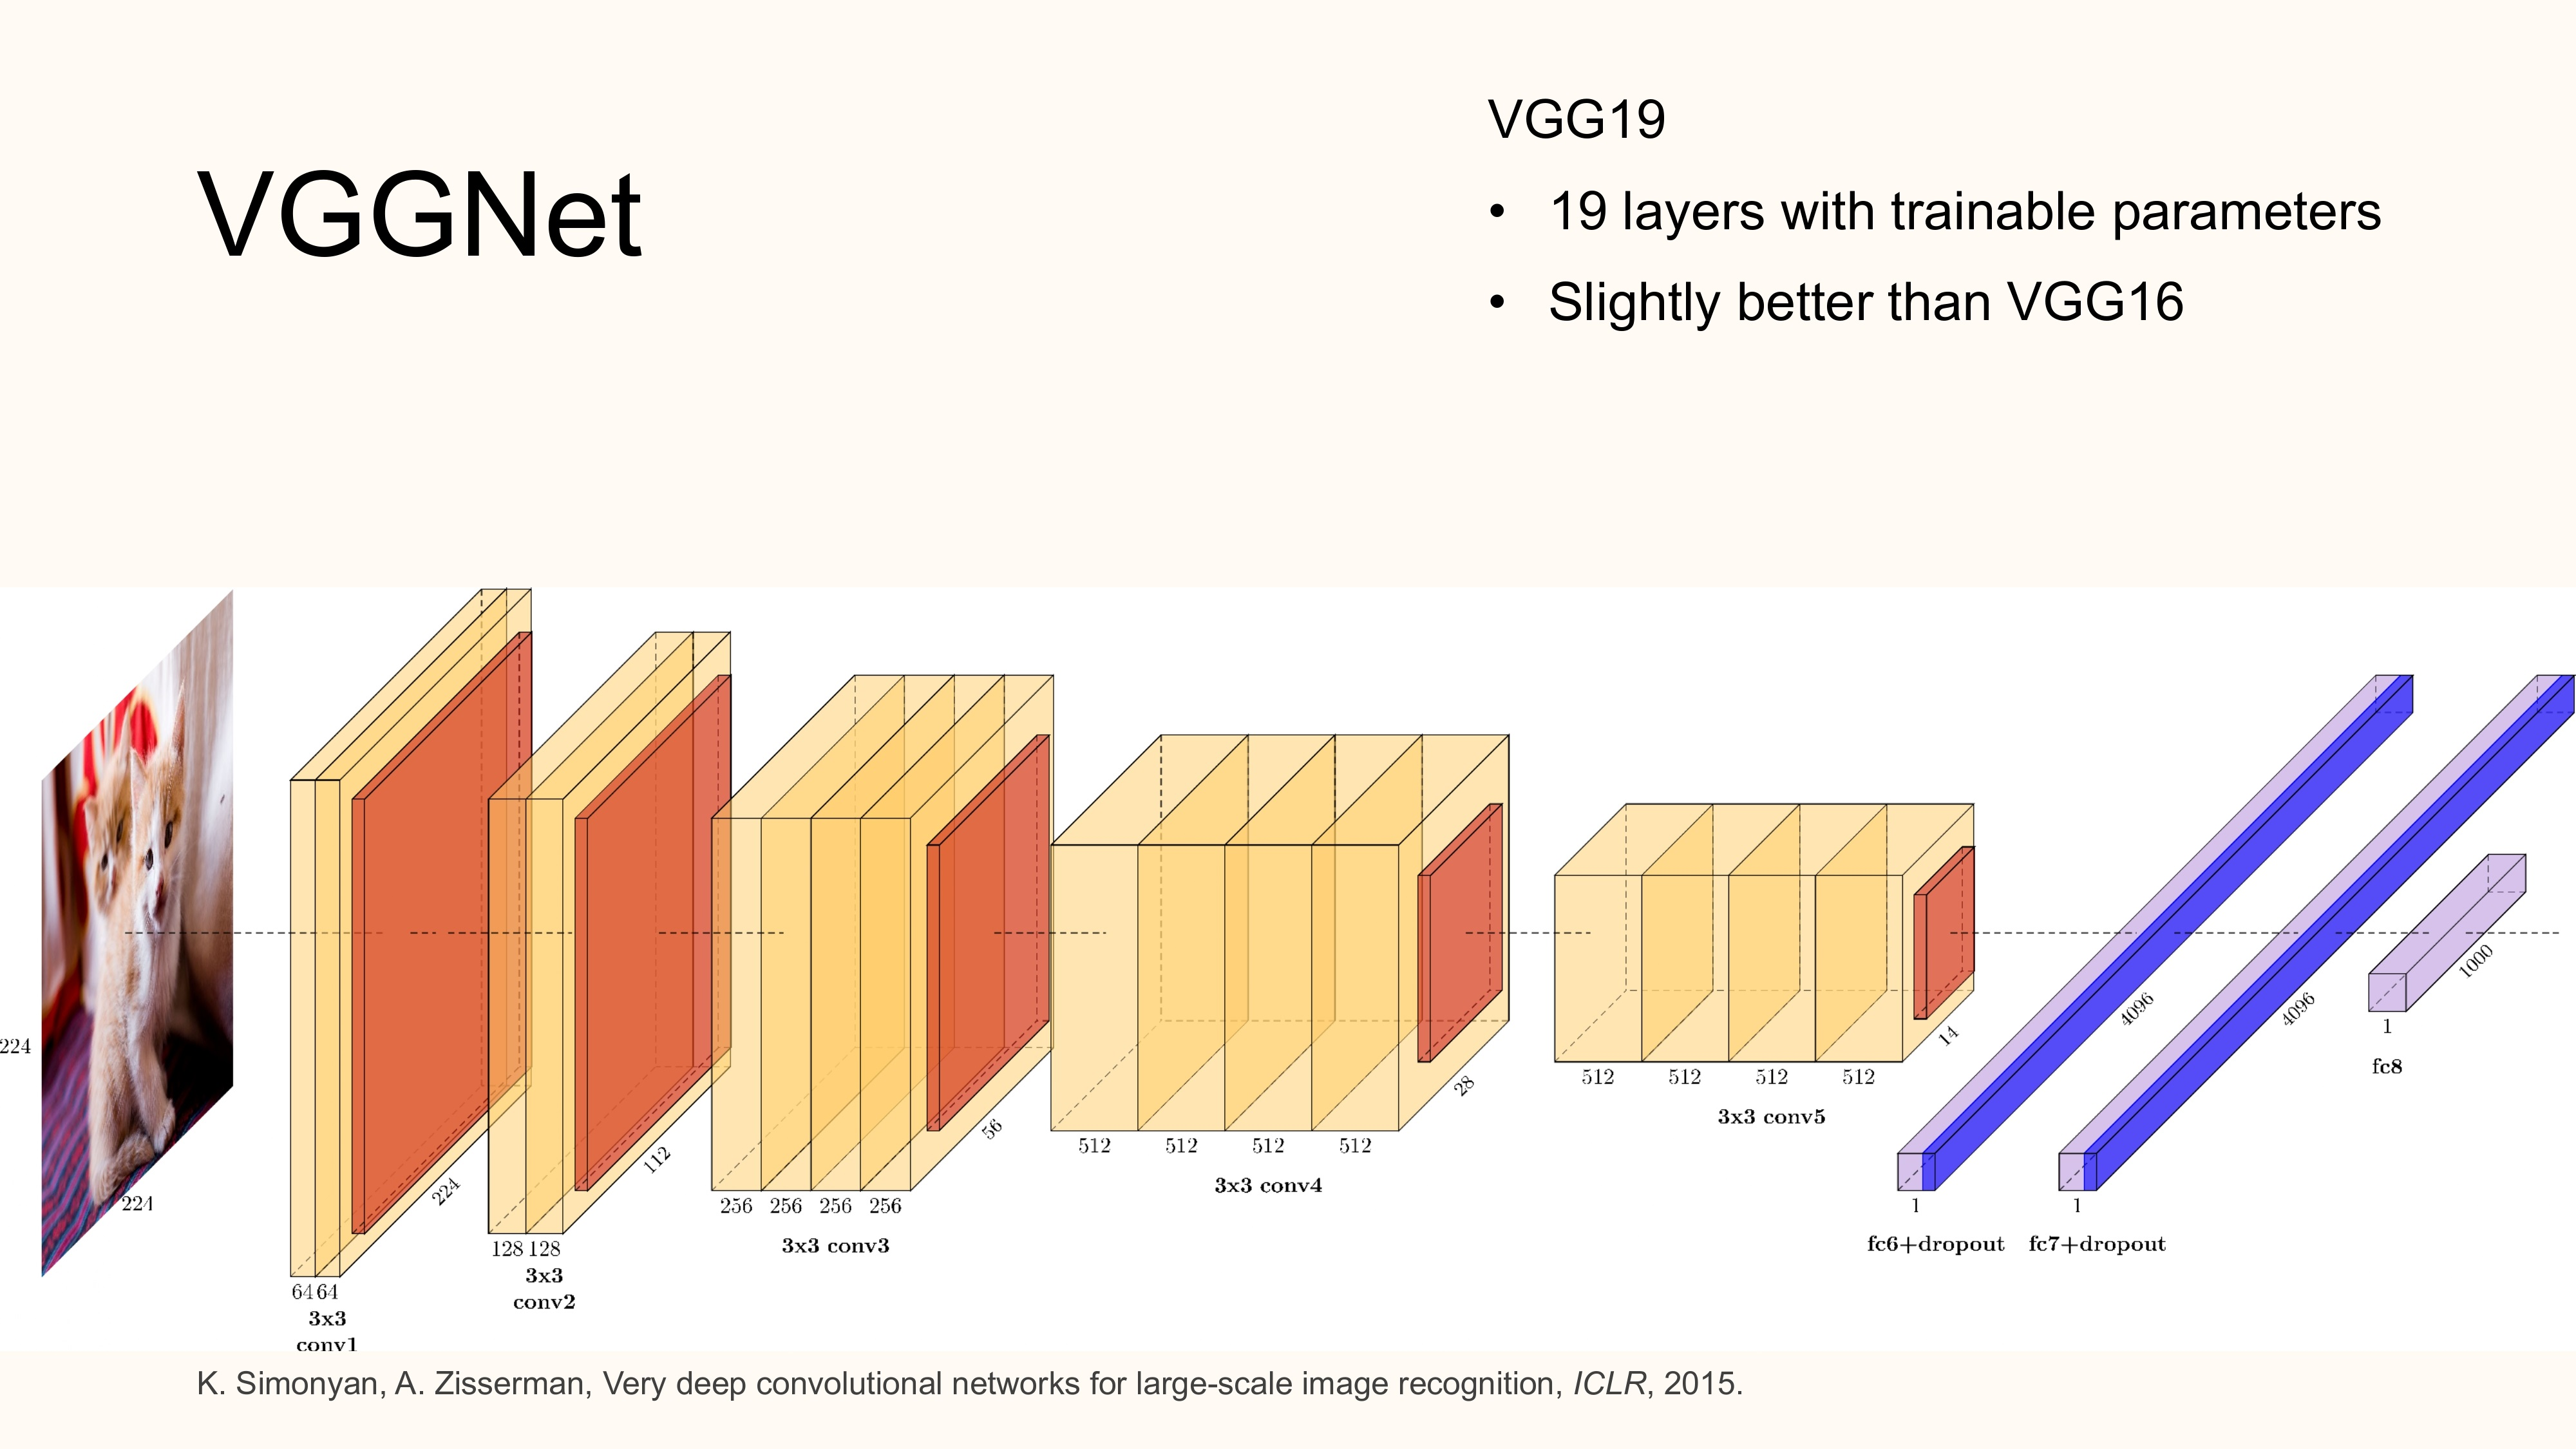
\includegraphics[width=1.0\textwidth]{.././assets/7.8.jpg}
    \end{figure}

    (K. Simonyan, A. Zisserman, Very deep convolutional networks for large-scale image recognition, ICLR, 2015.)
\end{definition}

\begin{definition}[7.9][VGGNet for Cifar10]
    \begin{figure}[H]
        \centering
        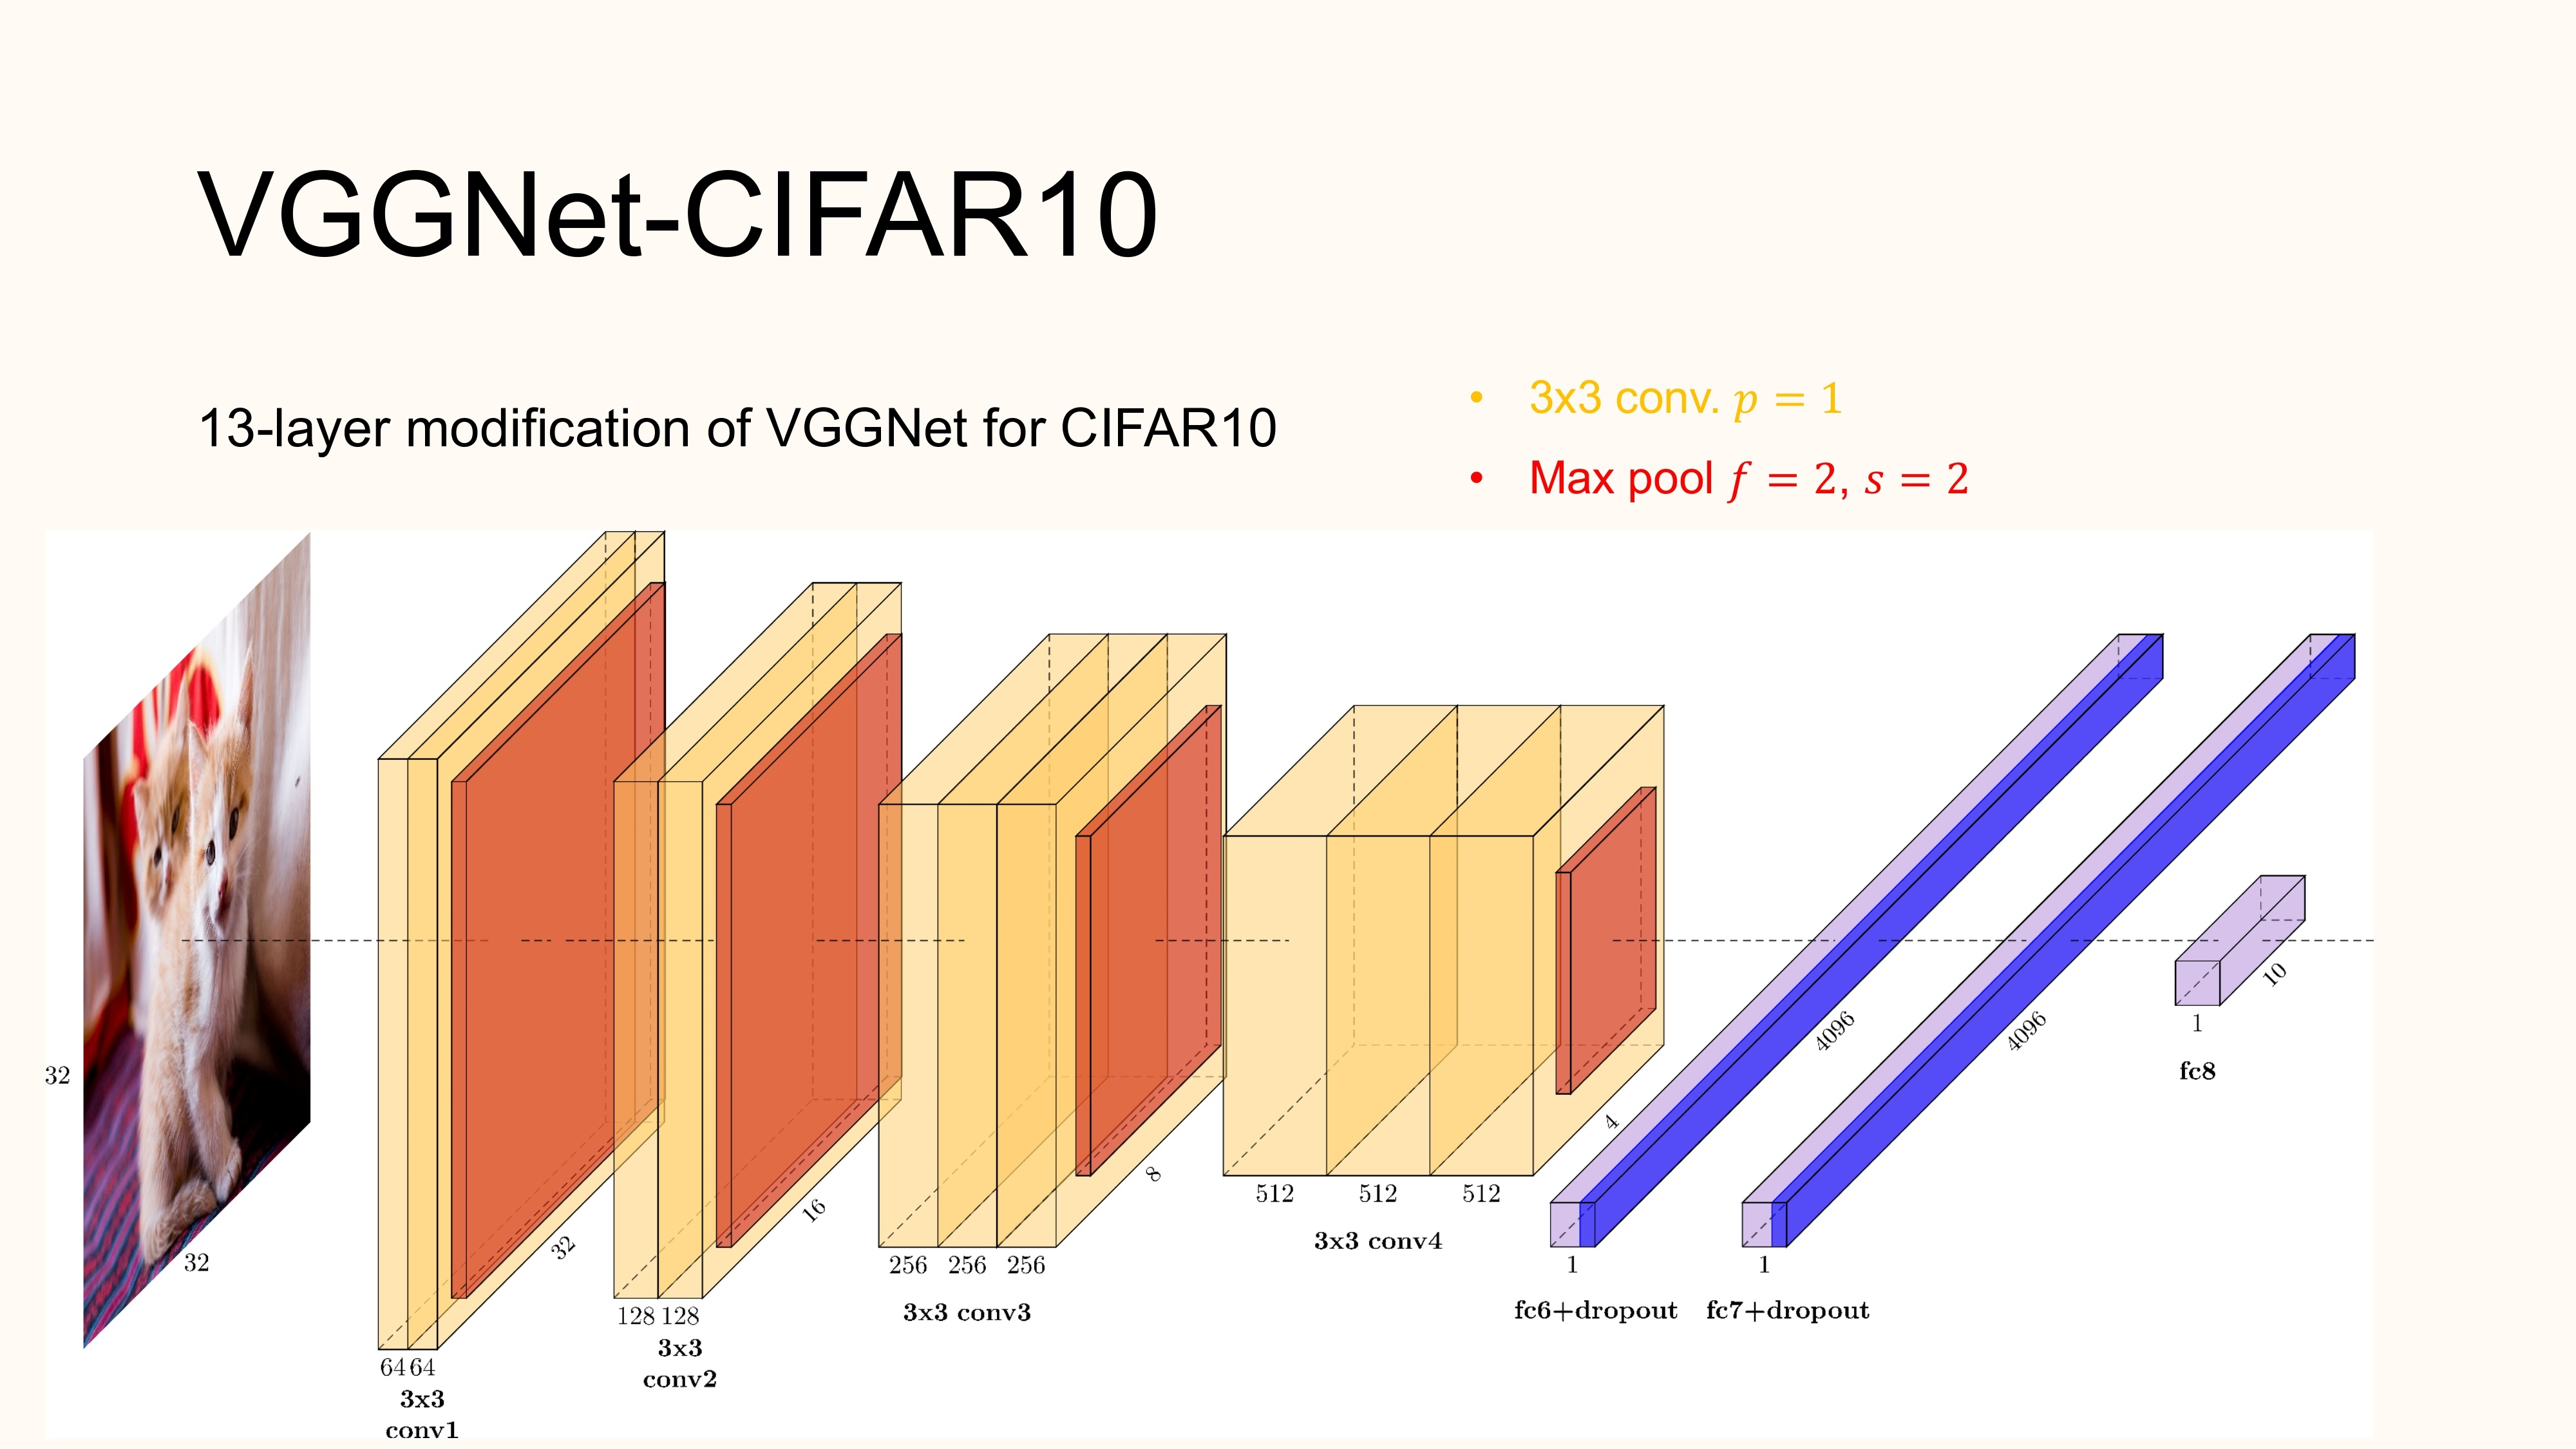
\includegraphics[width=1.0\textwidth]{.././assets/7.9.jpg}
    \end{figure}
\end{definition}

\begin{concept}[7.10][Architectural Contribution]
    Demonstrated simple deep CNNs can significantly improve upon AlexNet.

    In a sense, VGGNet represents the upper limit of the simple CNN architecture. (It is the best simple model.) Future architectures make gains through more complex constructions.

    Demonstrated effectiveness of stacked $3 \times 3$ convolutions over larger $5 \times 5$ or $11 \times 11$ convolutions. Large convolutions (larger than $5 \times 5$ ) are now uncommon.

    Due to its simplicity, VGGNet is one of the most common test subjects for testing something on deep CNNs.
\end{concept}

\section{NiN Network}

\begin{concept}[7.11][Linear layers have too many parameters.]
    Linear layers have too many parameters.

    \begin{itemize}
        \item
        AlexNet:

        Conv layer params: 2,469,696 (4%)\\
        Linear layer params: 58,631,144 (96%)\\
        Total params: 61,100,840
        \item
        VGG19:

        Conv layer params: 20,024,384 (14%)\\
        Linear layer params: 123,642,856 (86%)\\
        Total params: 143,667,240
    \end{itemize}
\end{concept}

\begin{definition}[7.12][Network in Network (NiN)]
    \begin{figure}[H]
        \centering
        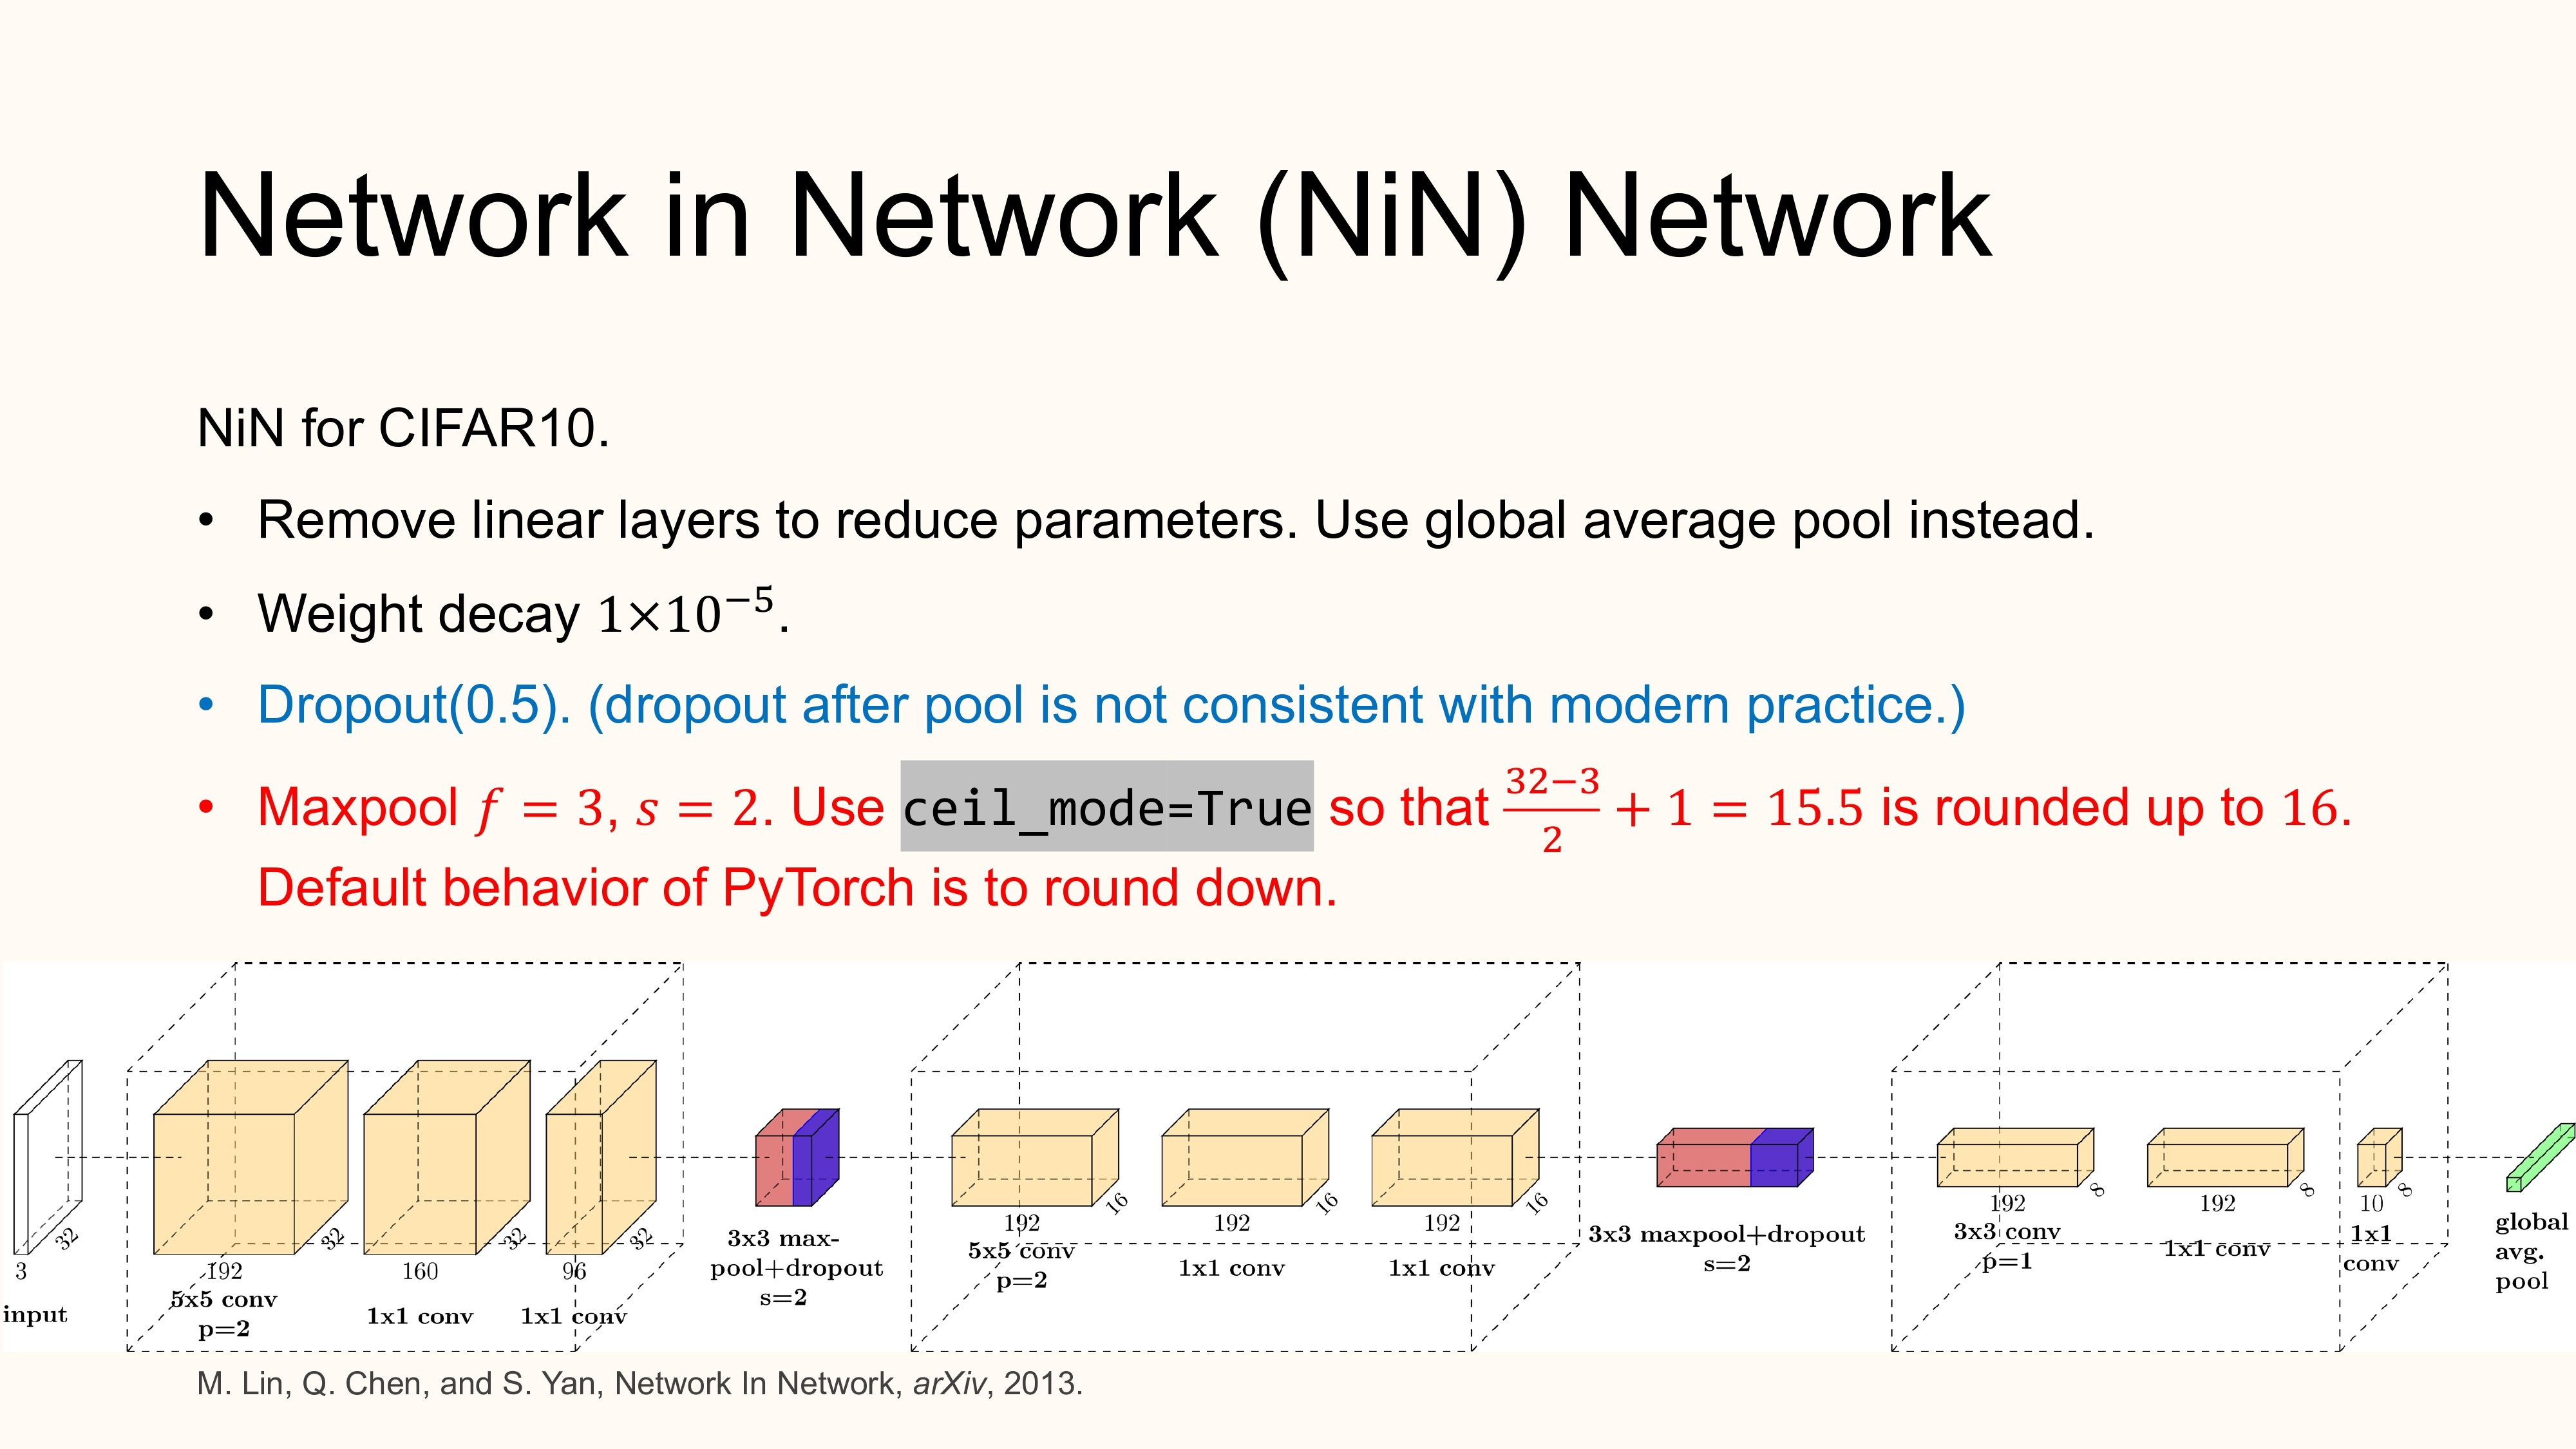
\includegraphics[width=1.0\textwidth]{.././assets/7.10.jpg}
    \end{figure}

    (M. Lin, Q. Chen, and S. Yan, Network In Network, arXiv, 2013.)
\end{definition}

\begin{concept}[7.13][$1 \times 1$ Convolution]
    A $1 \times 1$ convolution is like a fully connected layer acting independently and identically on each spatial location.

    \begin{figure}[H]
        \centering
        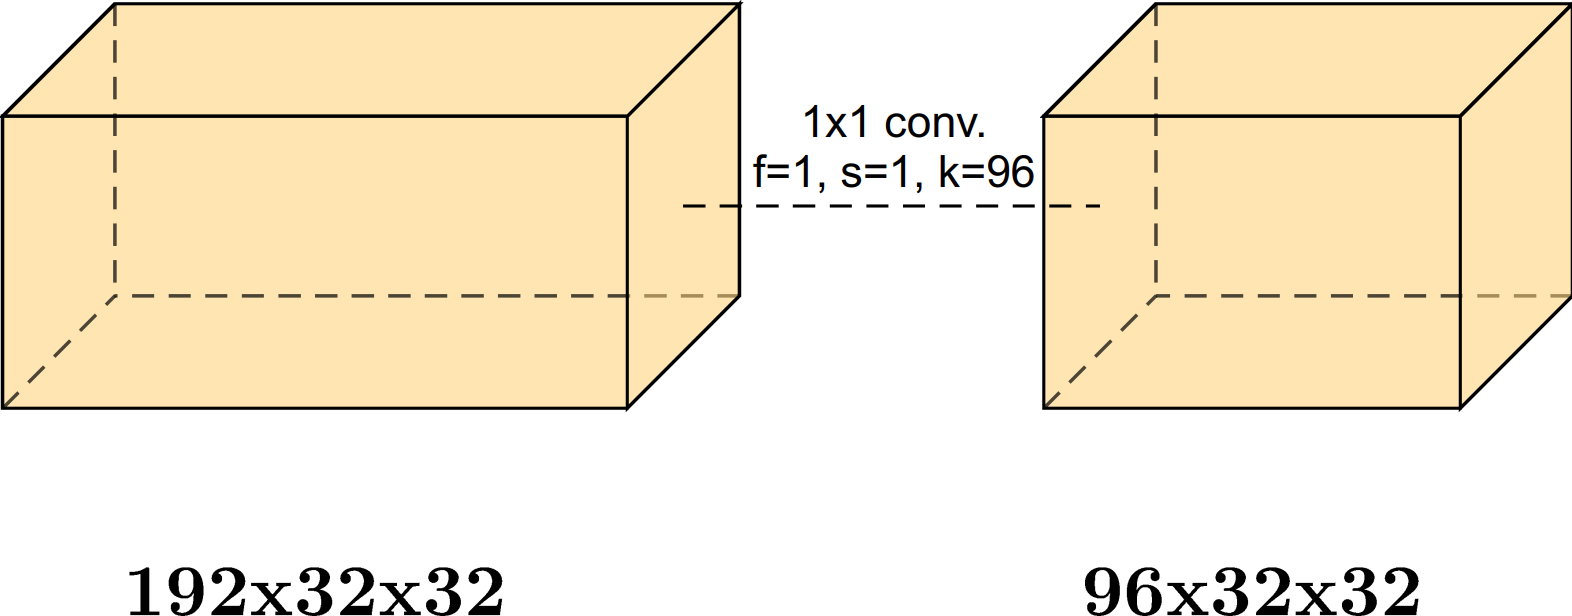
\includegraphics[width=0.7\textwidth]{.././assets/7.11.png}
    \end{figure}

    \begin{itemize}
        \item 96 filters act on 192 channels separately for each pixel
        \item $96 \times 192+96$ parameters for weights and biases
    \end{itemize}
\end{concept}

\begin{concept}[7.14][Regular Convolution Layer vs Network in Network]
    \textbf{Regular Convolution Layer}

    Input: $X \in \mathbb{R}^{C_{0} \times m \times n}$

    \begin{itemize}
        \item Select an $f \times f$ patch $\tilde{X}=X[:, i: i+f, j: j+f]$.
        \item Inner product $\tilde{X}$ and $w_{1}, \ldots, w_{C_{1}} \in \mathbb{R}^{C_{0} \times f \times f}$ and add bias $b_{1} \in \mathbb{R}^{C_{1}}$.
        \item Apply $\sigma$. (Output in $\mathbb{R}^{C_{1}}$.)
    \end{itemize}

    Repeat this for all patches. Output in $X \in \mathbb{R}^{C_{1} \times(m-f+1) \times(n-f+1)}$.
    Repeat this for all batch elements.

    \par\noindent\textcolor{gray}{\hdashrule{\textwidth}{0.4pt}{1pt 2pt}}

    \textbf{Network in Network}

    Input: $X \in \mathbb{R}^{c_{0} \times m \times n}$

    \begin{itemize}
        \item Select an $f \times f$ patch $\tilde{X}=X[:, i: i+f, j: j+f]$.
        \item Inner product $\tilde{X}$ and $w_{1}, \ldots, w_{C_{1}} \in \mathbb{R}^{C_{0} \times f \times f}$ and add bias $b_{1} \in \mathbb{R}^{C_{1}}$.
        \item Apply $\sigma$. (Output in $\mathbb{R}^{C_{1}}$.)
        \item Apply Linear $A_{A_{2}, b_{2}}(x)$ where $A_{2} \in \mathbb{R}^{C_{2} \times C_{1}}$ and $b_{2} \in \mathbb{R}^{C_{2}}$.
        \item Apply $\sigma$. (Output in $\mathbb{R}^{C_{2}}$.)
        \item Apply Linear $A_{A_{3}, b_{3}}(x)$ where $A_{3} \in \mathbb{R}^{C_{3} \times C_{2}}$ and $b_{3} \in \mathbb{R}^{C_{3}}$.
        \item Apply $\sigma$. (Output in $\mathbb{R}^{C_{3}}$.)
    \end{itemize}

    Repeat this for all patches. Output in $X \in \mathbb{R}^{C_{3} \times(m-f+1) \times(n-f+1)}$. Repeat this for all batch elements.
    Why is this equivalent to ($3 \times 3$ conv)-($1 \times 1$ conv)-($1 \times 1$ conv)?
\end{concept}

\begin{concept}[7.15][Global Average Pool]
    When using CNNs for classification, position of object is not important.

    The global average pool has no trainable parameters (linear layers have many) and it is translation invariant. Global average pool removes the spatial dependency.
\end{concept}

\begin{concept}[7.16][Architectural Contribution]
    Used $1 \times 1$ convolutions to increase the representation power of the convolutional modules.

    Replaced linear layer with average pool to reduce number of trainable parameters.

    First step in the trend of architectures becoming more abstract. Modern CNNs are built with smaller building blocks.
\end{concept}

\section{GoogLeNet}

\begin{definition}[7.17][GoogLeNet (Inception v1)]
    Utilizes the inception module. Structure inspired by NiN and name inspired by 2010 Inception movie meme.

    Used $1 \times 1$ convolutions.

    \begin{itemize}
        \item Increased depth adds representation power (improves ability to represent nonlinear functions).
        \item Reduce the number of channels before the expensive $3 \times 3$ and $5 \times 5$ convolutions, and thereby reduce number of trainable weights and computation time.
    \end{itemize}

    The name GoogLeNet is a reference to the authors' Google affiliation and is an homage to LeNet.

    \begin{figure}[H]
        \centering
        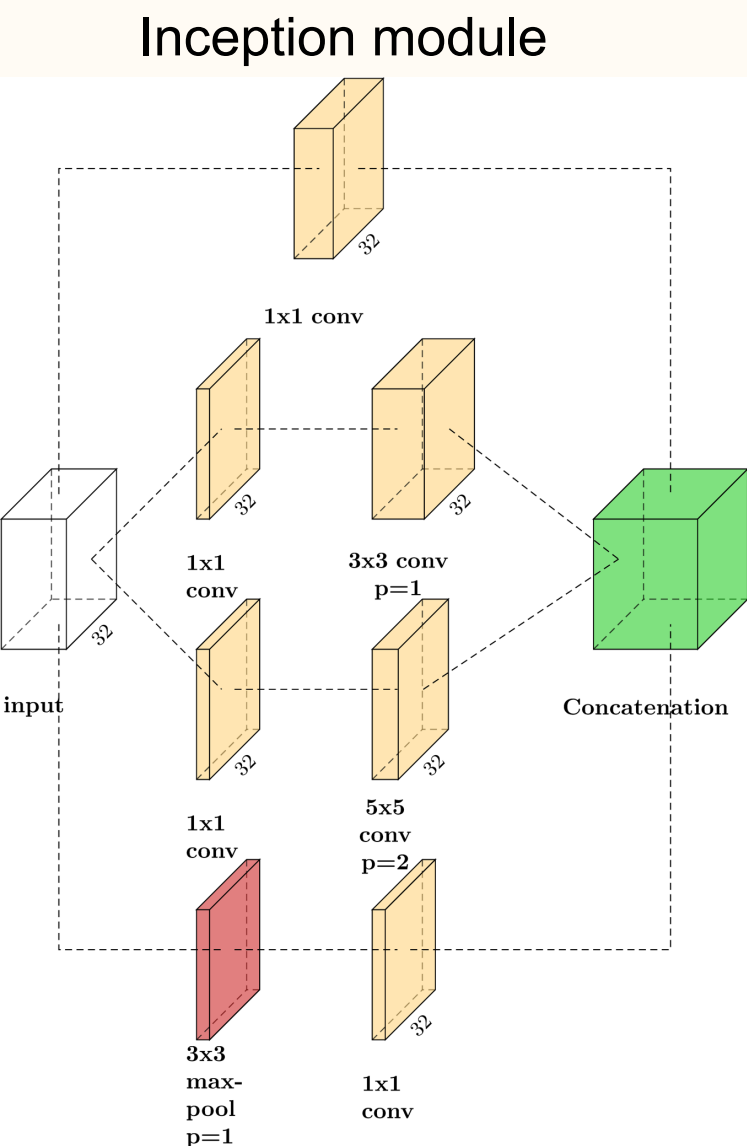
\includegraphics[width=0.6\textwidth]{.././assets/7.12.png}
    \end{figure}

    (C. Szegedy, W. Liu, Y. Jia, P. Sermanet, S. Reed, D. Anguelov, D. Erhan, V. Vanhoucke, and A. Rabinovich, Going deeper with convolutions, CVPR, 2015)

    \par\noindent\textcolor{gray}{\hdashrule{\textwidth}{0.4pt}{1pt 2pt}}

    \begin{figure}[H]
        \centering
        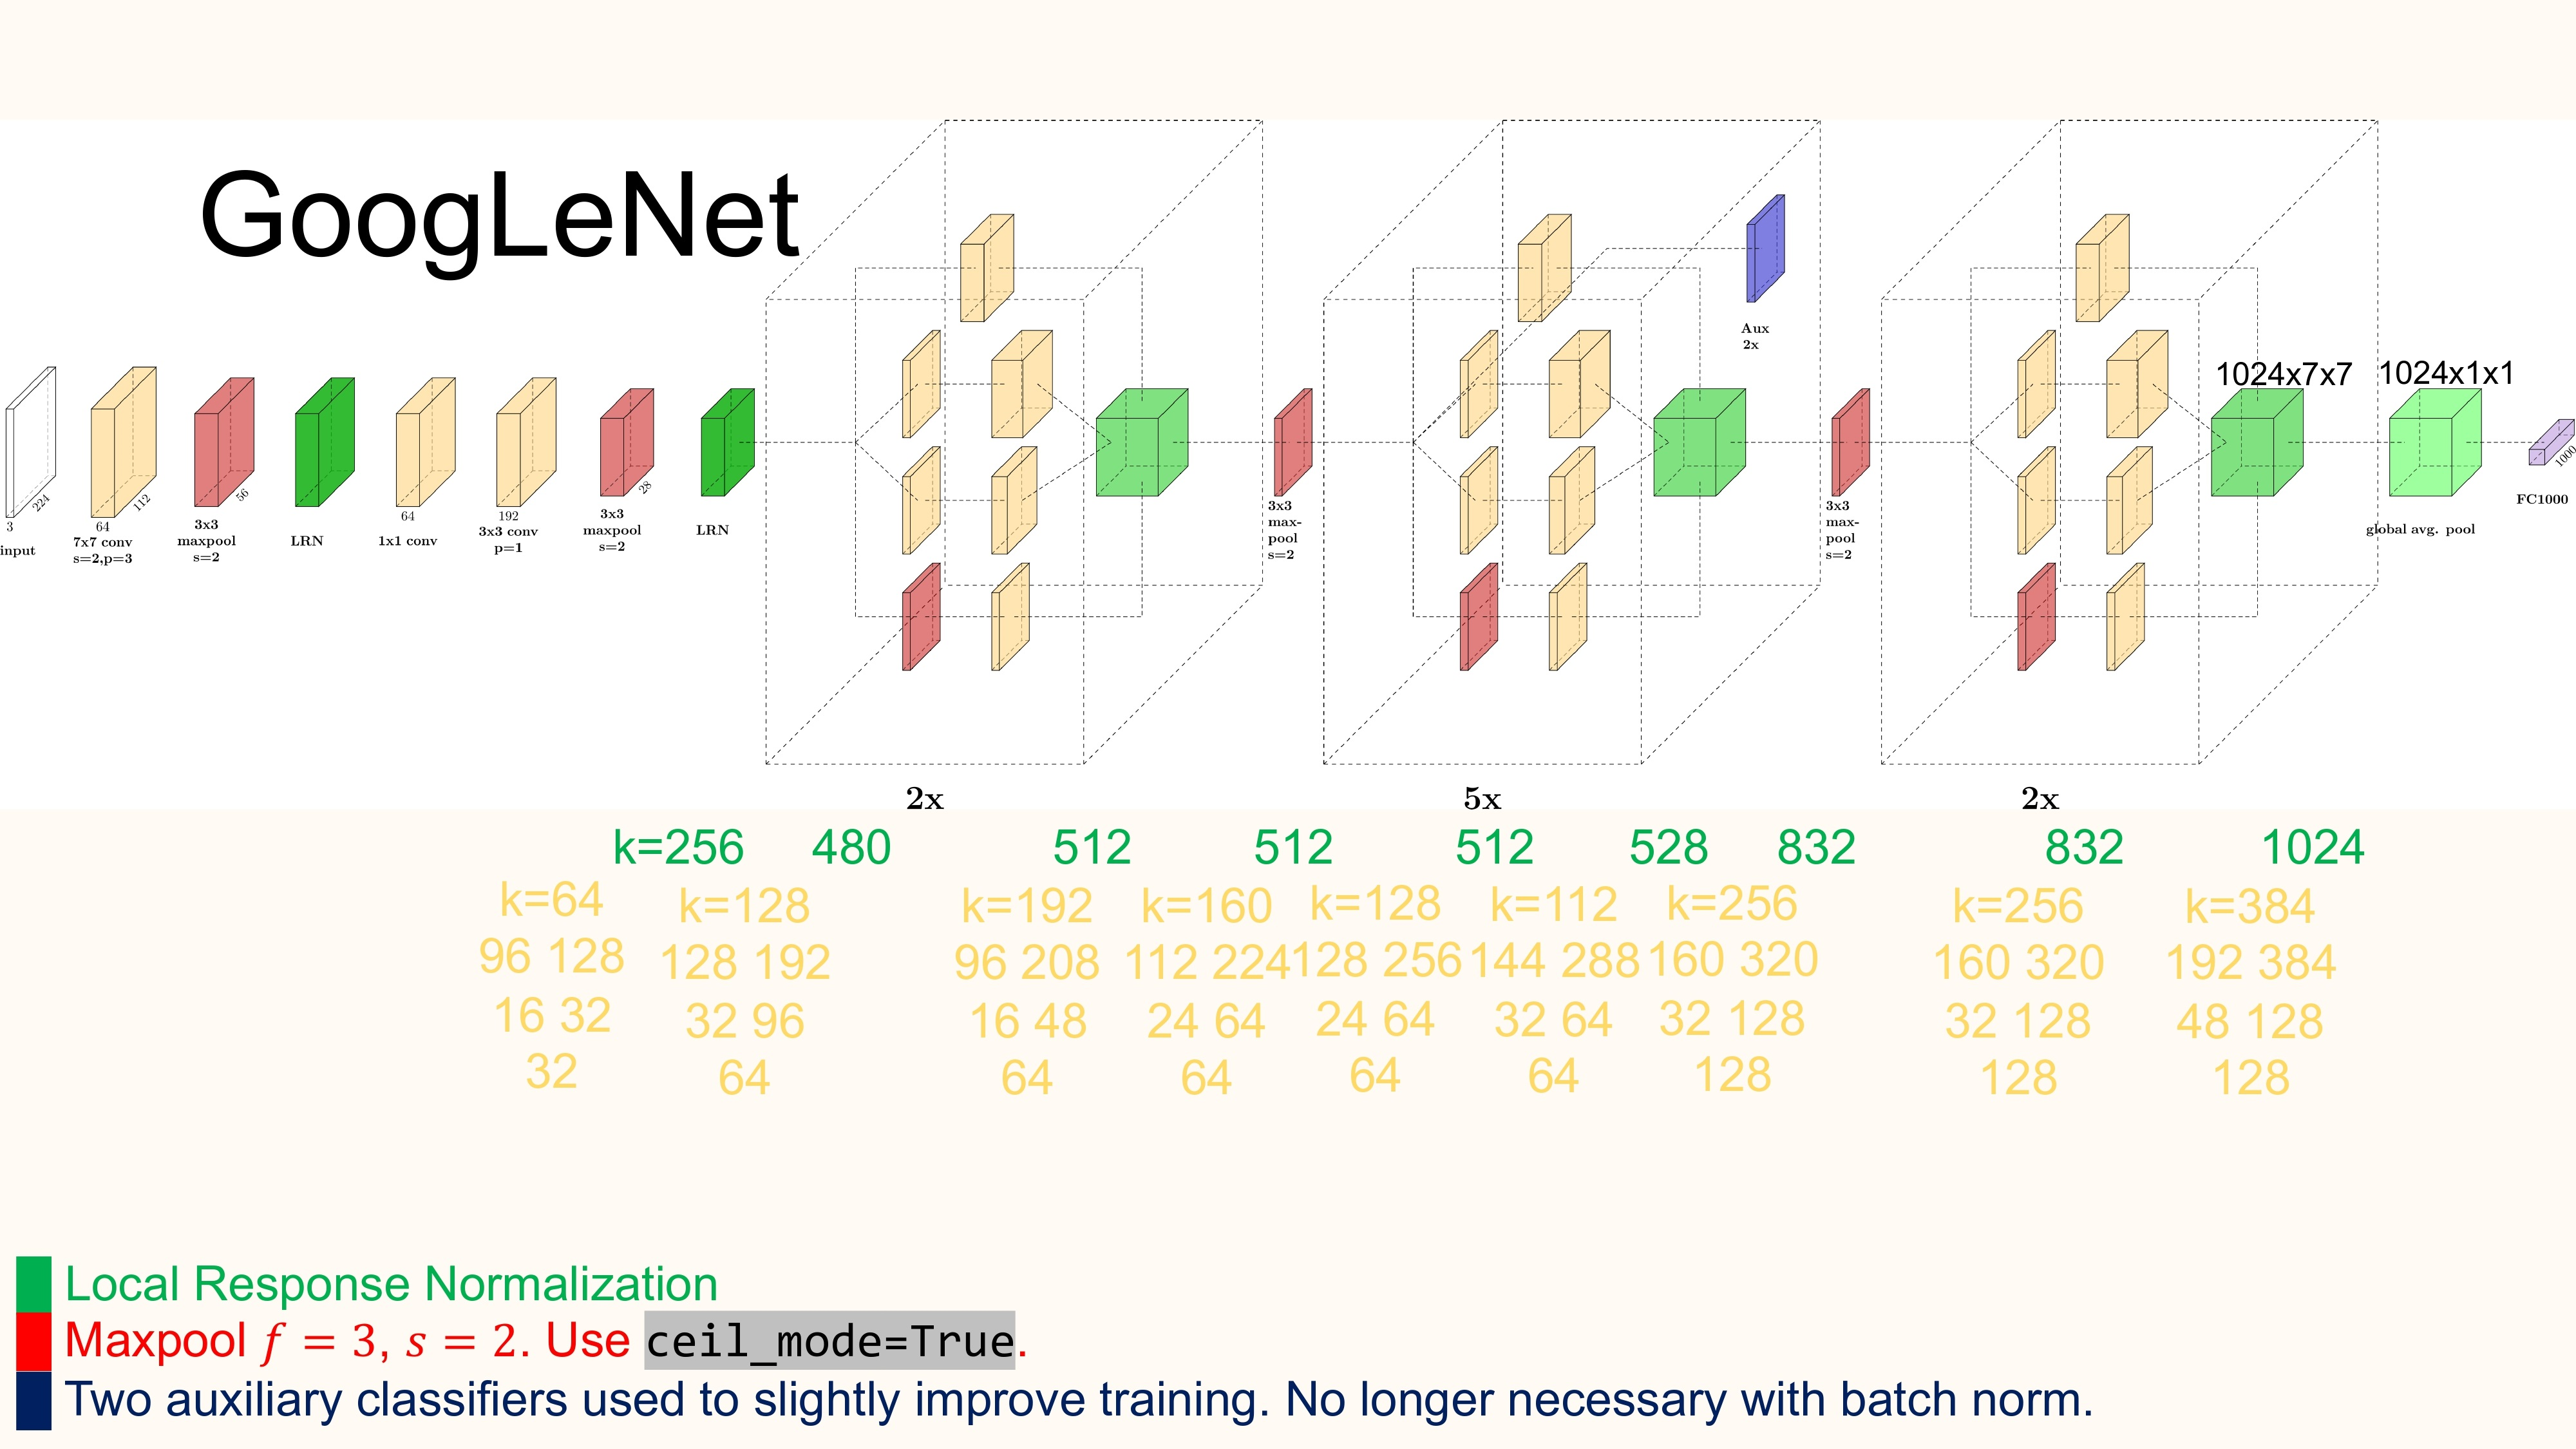
\includegraphics[width=1.0\textwidth]{.././assets/7.13.jpg}
    \end{figure}
\end{definition}

\begin{definition}[7.18][GoogLeNet for Cifar10]
    \begin{figure}[H]
        \centering
        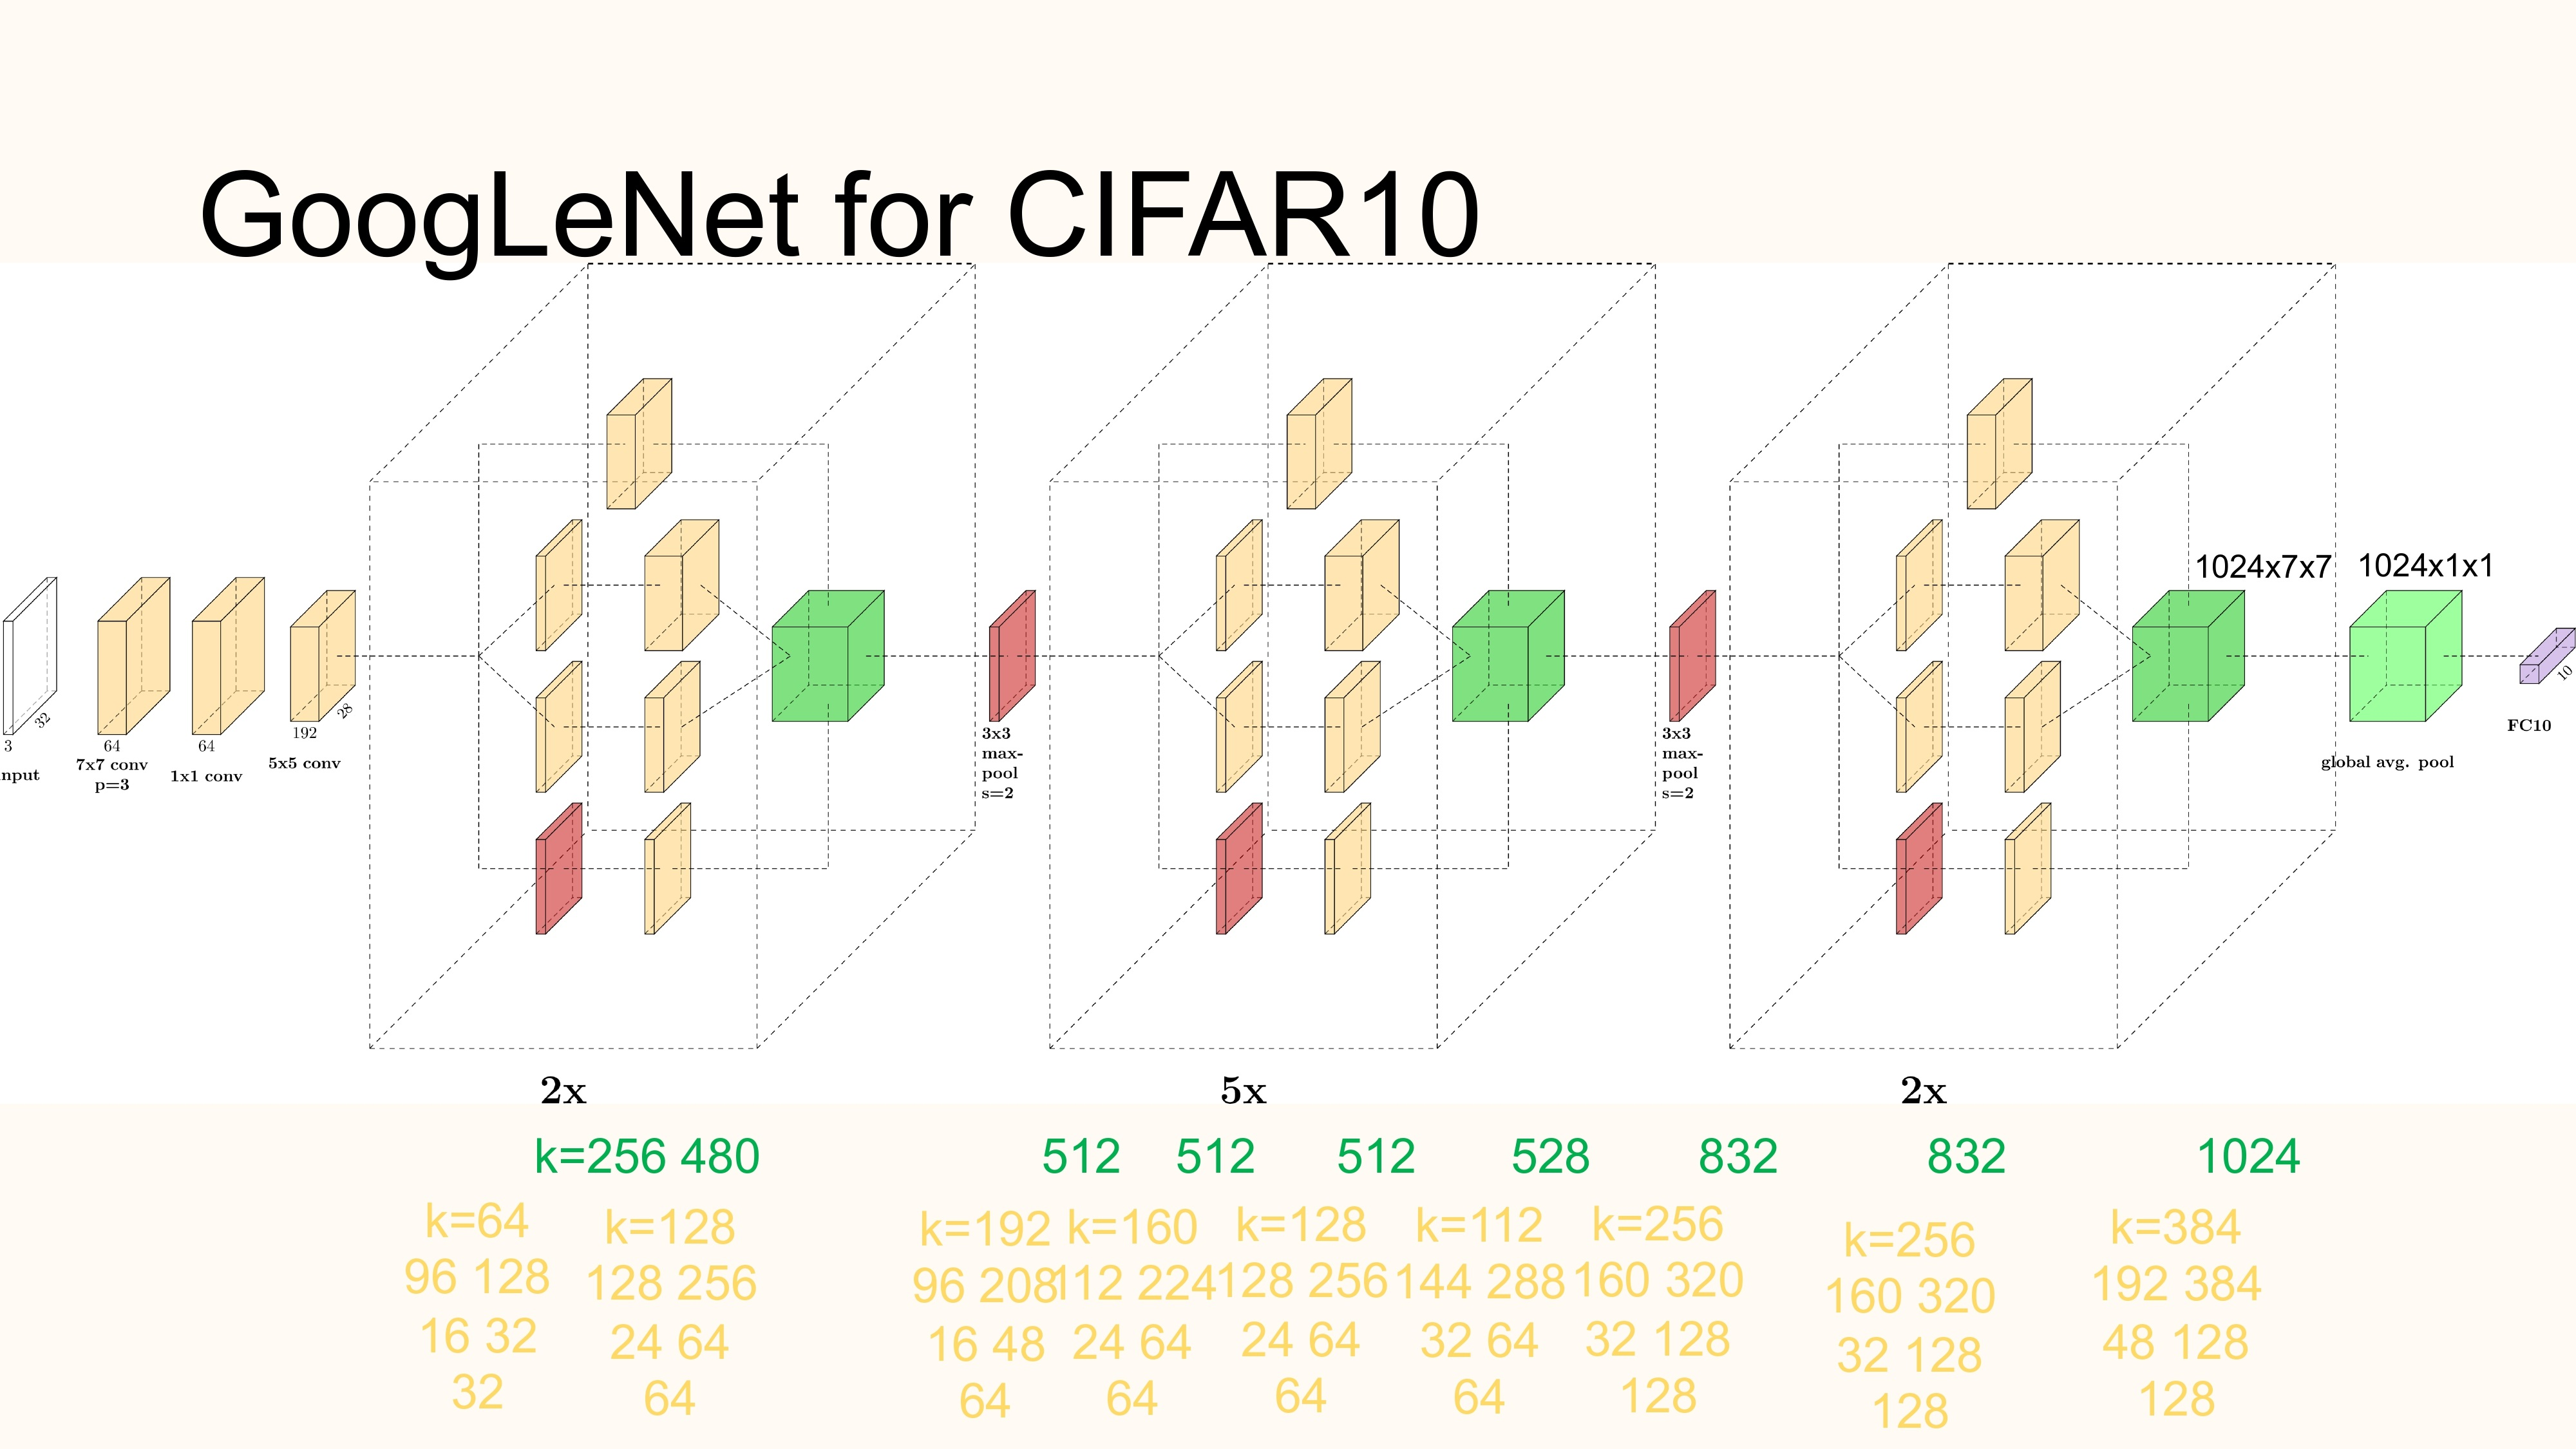
\includegraphics[width=1.0\textwidth]{.././assets/7.14.jpg}
    \end{figure}
\end{definition}

\begin{concept}[7.19][Architectural Contribution]
    Demonstrated that more complex modular neural network designs can outperform VGGNet's straightforward design.

    Together with VGGNet, demonstrated the importance of depth.

    Kickstarted the research into deep neural network architecture design.
\end{concept}

\section{ResNet}

\chapter*{Chapter 3 Code}

\href{https://drive.google.com/file/d/12O9fLasWDA-kOKBD-lE-1UhCl-PoDf0z/view?usp=sharing}{Chapter 3 Code}

\part{CNNs for Other Supervised Learning Tasks}

\chapter{CNNs for Other Supervised Learning Tasks}

\section{Inverse Problem}

\begin{definition}[8.1][Inverse Problem Model]
    In \textbf{inverse problems}, we wish to recover a signal $X_{\text {true }}$ given measurements $Y$. The unknown and the measurements are related through

    $$
    \mathcal{A}\left[X_{\text {true }}\right]+\varepsilon=Y,
    $$

    where $\mathcal{A}$ is often, but not always, linear, and $\varepsilon$ represents small error.

    The \textbf{forward model} $\mathcal{A}$ may or may not be known. In other words, the goal of an inverse problem is to find an \textbf{approximation of $\mathcal{A}^{-1}$}.

    In many cases, $\mathcal{A}$ is not even be invertible. In such cases, we can still hope to find an mapping that serves as an approximate inverse in practice.
\end{definition}

\begin{concept}[8.2][Inverse Problems via Deep Learning]
    In deep learning, we use a neural network to approximate the inverse mapping

    $$
    f_{\theta} \approx \mathcal{A}^{-1}
    $$

    i.e., we want $f_{\theta}(Y) \approx X_{\text {true }}$ for the measurements $X$ that we care about.

    If we have $X_{1}, \ldots, X_{N}$ and $Y_{1}, \ldots, Y_{N}$ (but no direct knowledge of $\mathcal{A}$ ), we can solve

    $$
    \underset{\theta \in \mathbb{R}^{p}}{\operatorname{minimize}} \sum_{i=1}^{N}\left\|f_{\theta}\left(Y_{i}\right)-X_{i}\right\|
    $$

    If we have $X_{1}, \ldots, X_{N}$ and knowledge of $\mathcal{A}$, we can solve

    $$
    \underset{\theta \in \mathbb{R}^{p}}{\operatorname{minimize}} \sum_{i=1}^{N}\left\|f_{\theta}\left[\mathcal{A}\left(X_{i}\right)\right]-X_{i}\right\|
    $$

    If we have $Y_{1}, \ldots, Y_{N}$ and knowledge of $\mathcal{A}$, we can solve

    $$
    \underset{\theta \in \mathbb{R}^{p}}{\operatorname{minimize}} \sum_{i=1}^{N}\left\|\mathcal{A}\left[f_{\theta}\left(Y_{i}\right)\right]-Y_{i}\right\|
    $$
\end{concept}

\subsection{Gaussian Denoising}

\begin{definition}[8.3][Gaussian Denoising]
    Given $X_{\text {true }} \in \mathbb{R}^{w \times h}$, we measure

    $$
    Y=X_{\text {true }}+\varepsilon
    $$

    where $\varepsilon_{i j} \sim \mathcal{N}\left(0, \sigma^{2}\right)$ is IID Gaussian noise. For the sake of simplicity, assume we know $\sigma$. Goal is to recover $X_{\text {true }}$ from $Y$.

    \textbf{Gaussian denoising} is the simplest setup in which the goal is to remove noise from the image. In more realistic setups, the noise model will be more complicated and the noise level $\sigma$ will be unknown.
\end{definition}

\begin{definition}[8.4][DnCNN]
    In 2017, Zhang et al. presented the \textbf{denoising convolutional neural networks (DnCNNs)}. They trained a 17-layer CNN $f_{\theta}$ to learn the noise with the loss

    $$
    \mathcal{L}(\theta)=\sum_{i=1}^{N}\left\|f_{\theta}\left(Y_{i}\right)-\left(Y_{i}-X_{i}\right)\right\|^{2}
    $$

    so that the clean recovery can be obtained with $Y_{i}-f_{\theta}\left(Y_{i}\right)$. (This is equivalent to using a residual connection from beginning to end.)

    \begin{figure}[H]
        \centering
        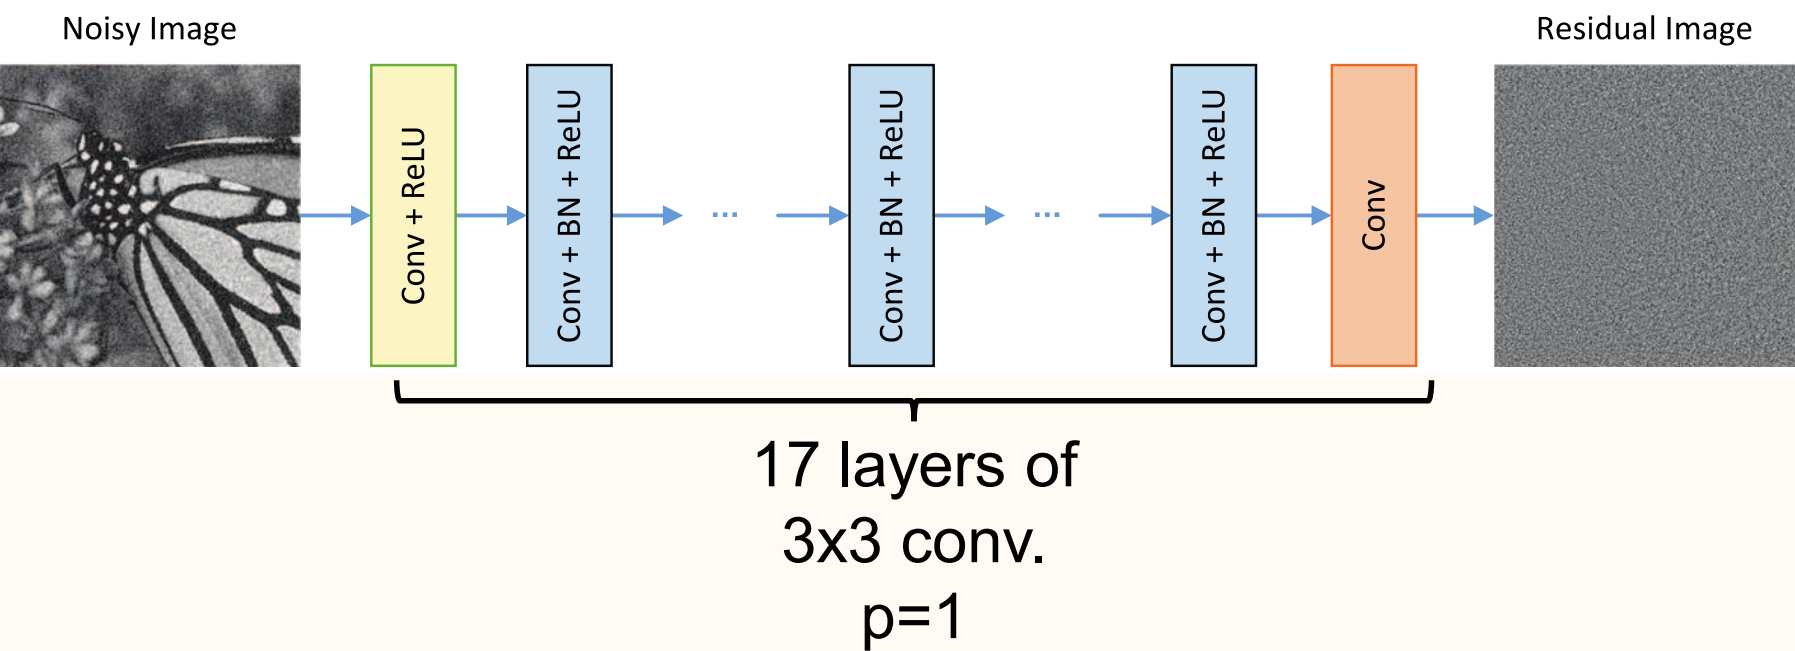
\includegraphics[width=0.7\textwidth]{.././assets/8.1.png}
    \end{figure}

    \par\noindent\textcolor{gray}{\hdashrule{\textwidth}{0.4pt}{1pt 2pt}}

    Image denoising is was an area with a large body of prior work. DnCNN dominated all prior approaches that were not based on deep learning.

    Nowadays, all state-of-the-art denoising algorithms are based on deep learning.

    \begin{figure}[H]
        \centering
        \includegraphics[width=1.0\textwidth]{.././assets/8.2.png}
    \end{figure}

    (K. Zhang, W. Zuo, Y. Chen, D. Meng, and L. Zhang, Beyond a Gaussian denoiser: Residual learning of deep CNN for image denoising, IEEE TIP, 2017.)
\end{definition}

\subsection{Image Super-Resolution}

\begin{definition}[8.5][Image Super-Resolution]
    Given $X_{\text {true }} \in \mathbb{R}^{w \times h}$, we measure

    $$
    Y=\mathcal{A}\left(X_{\text {true }}\right)
    $$

    where $\mathcal{A}$ is a "downsampling" operator. So $Y \in \mathbb{R}^{w_{2} \times h_{2}}$ with $w_{2}<w$ and $h_{2}<h$. Goal is to recover $X_{\text {true }}$ from $Y$.

    In the simplest setup, $\mathcal{A}$ is an average pool operator with $r \times r$ kernel and a stride $r$.
\end{definition}

\begin{definition}[8.6][SRCNN]
    In 2015, Dong et al. presented super-resolution convolutional neural network (SRCNN). They trained a 3-layer $\operatorname{CNN} f_{\theta}$ to learn the high-resolution reconstruction with the loss

    $$
    \mathcal{L}(\theta)=\sum_{i=1}^{N}\left\|f_{\theta}\left(\tilde{Y}_{i}\right)-X_{i}\right\|^{2}
    $$

    where $\tilde{Y}_{i} \in \mathbb{R}^{w \times h}$ is an upsampled version of $Y_{i} \in \mathbb{R}^{(w / r) \times(h / r)}$, i.e., $\tilde{Y}_{i}$ has the same number of pixels as $X_{i}$, but the image is pixelated or blurry. The goal is to have $f_{\theta}\left(\tilde{Y}_{i}\right)$ be a sharp reconstruction.

    \begin{figure}[H]
        \centering
        \includegraphics[width=0.7\textwidth]{.././assets/8.3.png}
    \end{figure}

    \par\noindent\textcolor{gray}{\hdashrule{\textwidth}{0.4pt}{1pt 2pt}}

    SRCNN showed that simple learning based approaches can match the state-of the art performances of superresolution task.

    \begin{figure}[H]
        \centering
        \includegraphics[width=1.0\textwidth]{.././assets/8.4.png}
    \end{figure}

    (C. Dong, C. C. Loy, K. He, and X. Tang, Image super-resolution using deep convolutional networks, IEEE TPAMI, 2015.)
\end{definition}

\begin{definition}[8.7][VDSR]
    In 2016, Kim et al. presented VDSR. They trained a 20-layer CNN with a residual connection $f_{\theta}$ to learn the high-resolution reconstruction with the loss

    $$
    \mathcal{L}(\theta)=\sum_{i=1}^{N}\left\|f_{\theta}\left(\tilde{Y}_{i}\right)-X_{i}\right\|^{2}
    $$

    The residual connection was the key insight that enabled the training of much deeper CNNs.

    \begin{figure}[H]
        \centering
        \includegraphics[width=0.7\textwidth]{.././assets/8.5.png}
    \end{figure}

    \par\noindent\textcolor{gray}{\hdashrule{\textwidth}{0.4pt}{1pt 2pt}}

    VDSR dominated all prior approaches not based on deep learning.
    Showed that simple learning based approaches can batch the state-of theart performances of super-resolution task.

    \begin{figure}[H]
        \centering
        \includegraphics[width=1.0\textwidth]{.././assets/8.6.png}
    \end{figure}

    (J. Kim, J. K. Lee, and K. M. Lee, Accurate image super-resolution using very deep convolutional networks, CVPR, 2016.)
\end{definition}

\subsection{Other Examples}

\begin{example}[8.8][SRGAN]
    \begin{figure}[H]
        \centering
        \includegraphics[width=1.0\textwidth]{.././assets/8.7.png}
    \end{figure}

    \begin{figure}[H]
        \centering
        \includegraphics[width=1.0\textwidth]{.././assets/8.8.png}
    \end{figure}

    \begin{figure}[H]
        \centering
        \includegraphics[width=1.0\textwidth]{.././assets/8.9.png}
    \end{figure}

    (C. Ledig, L. Theis, F. Huszar, J. Caballero, A. Cunningham, A. Acosta, A. Aitken, A. Tejani, J. Totz, Z. Wang, and W. Shi, Photo-realistic single image super-resolution using a generative adversarial network, CVPR, 2017.)
\end{example}

\begin{example}[8.9][Image Colorization]
    \begin{figure}[H]
        \centering
        \includegraphics[width=1.0\textwidth]{.././assets/8.10.png}
    \end{figure}

    (R. Zhang, P. Isola, and A. A. Efros, Colorful image colorization, ECCV, 2016.)
\end{example}

\begin{example}[8.10][Image Inpainting]
    \begin{figure}[H]
        \centering
        \includegraphics[width=1.0\textwidth]{.././assets/8.11.png}
    \end{figure}

    \begin{figure}[H]
        \centering
        \includegraphics[width=1.0\textwidth]{.././assets/8.12.png}
    \end{figure}

    (J. Yu, Z. Lin, J. Yang, X. Shen, X. Lu, and T. S. Huang, Generative image inpainting with contextual attention, CVPR, 2018.)
\end{example}

\section{Operations Increasing Spatial Dimensions}

\begin{concept}[8.11][Operations Increasing Spatial Dimensions]
    In image classification tasks, the spatial dimensions of neural networks often decrease as the depth progresses.

    This is because we are trying to forget location information. (In classification, we care about what is in the image, but we do not where it is in the image.)

    However, there are many networks for which we want to increase the spatial dimension:

    \begin{itemize}
        \item Linear layers
        \item Upsampling
        \item Transposed convolution
    \end{itemize}
\end{concept}

\subsection{Transposed convolution}

\begin{concept}[8.12][Linear Operator $\cong$ Matrix]
    Core tenet of linear algebra: matrices are linear operators and linear operators are matrices.

    Let $f: \mathbb{R}^{n} \rightarrow \mathbb{R}^{m}$ be linear, i.e.,

    $$
    f(x+y)=f(x)+f(y) \text { and } f(\alpha x)=\alpha f(x)
    $$

    for all $x, y \in \mathbb{R}^{n}$ and $\alpha \in \mathbb{R}$.

    There exists a matrix $A \in \mathbb{R}^{m \times n}$ that represents $f: \mathbb{R}^{n} \rightarrow \mathbb{R}^{m}$, i.e.,

    $$
    f(x)=A x
    $$

    for all $x \in \mathbb{R}^{n}$.

    Let $e_{i}$ be the $i$-th unit vector, i.e., $e_{i}$ has all zeros elements except entry 1 in the $i$-th coordinate.

    Given a linear $f: \mathbb{R}^{n} \rightarrow \mathbb{R}^{m}$, we can find the matrix

    $$
    A=\left[\begin{array}{llll}
    A_{;, 1} & A_{;, 2} & \cdots & A_{;, n}
    \end{array}\right] \in \mathbb{R}^{m \times n}
    $$

    representing $f$ with

    $$
    f\left(e_{j}\right)=A e_{j}=A_{;, j}
    $$

    for all $j=1, \ldots, n$, or with

    $$
    e_{i}^{\top} f\left(e_{j}\right)=e_{i}^{\top} A e_{j}=A_{i, j}
    $$

    for all $i=1, \ldots, m$ and $j=1, \ldots, n$.
\end{concept}

\begin{concept}[8.13][Linear Operator $\ncong$ Matrix]
    In applied mathematics and machine learning, there are many setups where explicitly forming the matrix representation $A \in \mathbb{R}^{m \times n}$ is costly, even though the matrix-vector products $A x$ and $A^{\top} y$ are efficient to evaluate.

    In machine learning, convolutions are the primary example. Other areas, linear operators based on FFTs are the primary example.

    In such setups, the matrix representation is still a useful conceptual tool, even if we never intend to form the matrix.
\end{concept}

Given a matrix $A$, the transpose $A^{\top}$ is obtained by flipping the row and column dimensions, i.e., $\left(A^{\top}\right)_{i j}=(A)_{j i}$.
However, using this definition is not always the most effective when understanding the action of $A^{\top}$.

Another approach is to use the adjoint view. Since

$$
y^{\top}(A x)=\left(A^{\top} y\right)^{\top} x
$$

for any $x \in \mathbb{R}^{n}$ and $y \in \mathbb{R}^{m}$, understand the action of $A^{\top}$ by finding an expression of the form

$$
y^{\top} A x=\sum_{j=1}^{n}(\text { something })_{j} x_{j}=\left(A^{\top} y\right)^{\top} x
$$

\begin{example}[8.14][1D Transpose Convolution]
    Consider the 1D convolution represented by $A \in \mathbb{R}^{(n-f+1) \times n}$ defined with a given $w \in \mathbb{R}^{f}$ and

    $$
    A=\left[\begin{array}{cccccccc}
    w_{1} & \cdots & w_{f} & 0 & \cdots & & & 0 \\
    0 & w_{1} & \cdots & w_{f} & 0 & \cdots & & 0 \\
    0 & 0 & w_{1} & \cdots & w_{f} & 0 & \cdots & 0 \\
    \vdots & & & \ddots & & \ddots & & \vdots \\
    0 & & \cdots & 0 & w_{1} & \cdots & w_{f} & 0 \\
    0 & & \cdots & 0 & 0 & w_{1} & \cdots & w_{f}
    \end{array}\right]
    $$

    Then we have

    $$
    (A x)_{j}=\sum_{i=1}^{f} w_{i} x_{j+i-1}
    $$

    \par\noindent\textcolor{gray}{\hdashrule{\textwidth}{0.4pt}{1pt 2pt}}

    and we have the following formula which coincides with transposing the matrix $A$.

    $$
    \begin{aligned}
    y^{\top} A x & =\sum_{j=1}^{n-f+1} y_{j} \sum_{i=1}^{f} w_{i} x_{j+i-1} \\
    & =\sum_{j=1}^{n-f+1} \sum_{i=1}^{f} y_{j} w_{i} x_{j+i-1} \sum_{k=1}^{n} \mathbf{1}_{\{k=j+i-1\}} \\
    & =\sum_{k=1}^{n} \sum_{j=1}^{n-f+1} \sum_{i=1}^{f} y_{j} w_{i} x_{k} \mathbf{1}_{\{k-j+1=i\}} \\
    & =\sum_{k=1}^{n} x_{k} \sum_{j=1}^{n-f+1} \sum_{i=1}^{f} w_{k-j+1} y_{j} \mathbf{1}_{\{k-j+1=i\}} \\
    & =\sum_{k=1}^{n} x_{k} \sum_{j=1}^{n-f+1} w_{k-j+1} y_{j} \sum_{i=1}^{f} \mathbf{1}_{\{k-j+1=i\}} \\
    & =\sum_{k=1}^{n} x_{k} \sum_{j=1}^{n-f+1} w_{k-j+1} y_{j} \mathbf{1}_{\{1 \leq k-j+1 \leq f\}} \\
    & =\sum_{k=1}^{n} x_{k} \sum_{j=1}^{n-f+1} w_{k-j+1} y_{j} \mathbf{1}_{\{j \leq k\}} \mathbf{1}_{\{k-f+1 \leq j\}} \\
    & =\sum_{k=1}^{n} x_{k} \sum_{j=\max (k-f+1,1)}^{\min (n-f+1, k)} w_{k-j+1} y_{j}=\left(A^{\top} y\right)^{\top} x \\
    \end{aligned}
    $$
\end{example}

\begin{definition}[8.15][Transposed Convolution]
    In transposed convolution, input neurons additively distribute values to the output via the kernel.
    Before people noticed that this is the transpose of convolution, the names backwards convolution and deconvolution were used.

    For each input neuron, multiply the kernel and add (accumulate) the value in the output.
    Can accommodate strides, padding, and multiple channels.

    \begin{figure}[H]
        \centering
        \includegraphics[width=1.0\textwidth]{.././assets/8.13.png}
    \end{figure}

    \begin{figure}[H]
        \centering
        \includegraphics[width=1.0\textwidth]{.././assets/8.14.png}
    \end{figure}
\end{definition}

\begin{itemize}
    \item Convolution Visualized
\end{itemize}

\begin{figure}[H]
    \centering
    \includegraphics[width=0.5\textwidth]{.././assets/8.15.gif}
\end{figure}

\begin{itemize}
    \item Transpose Convolution Visualized
\end{itemize}

\begin{figure}[H]
    \centering
    \includegraphics[width=1.0\textwidth]{.././assets/8.16.gif}
\end{figure}

\begin{definition}[8.16][2D Transpose Convolution Layer (Formal Definition)]
    \begin{itemize}
        \item $B$ : batch size
        \item $C_{\text{in}}$ : \# of input channels
        \item $C_{\text{out}}$ : \# of output channels
        \item $m, n$ : \# of vertical and horizontal indices of input
        \item $f_1, f_2$ : \# of vertical and horizontal indices of filter
    \end{itemize}

    \par\noindent\textcolor{gray}{\hdashrule{\textwidth}{0.4pt}{1pt 2pt}}

    \begin{itemize}
        \item Input tensor: $Y \in \mathbb{R}^{B \times C_{\mathrm{in}} \times m \times n}$
        \item Output tensor: $X \in \mathbb{R}^{B \times C_{\text {out }} \times\left(m+f_{1}-1\right) \times\left(n+f_{2}-1\right)}$
        \item Filter $w \in \mathbb{R}^{C_{\text {in }} \times C_{\text {out }} \times f_{1} \times f_{2}}$
        \item Bias $b \in \mathbb{R}^{C_{\text {out }}}$ (If \verb|bias=False|, then $b=0$.) 
    \end{itemize}

    \par\noindent\textcolor{gray}{\hdashrule{\textwidth}{0.4pt}{1pt 2pt}}

    \begin{verbatim}
    def trans_conv(Y, w, b):
        c_in, c_out, f1, f2 = w.shape
        batch, c_in, m, n = Y.shape
        X = torch.zeros(batch, c_out, m + f1 - 1, n + f2 - 1)
        for k in range(c_in):
            for i in range(Y.shape[2]):
                for j in range(Y.shape[3]):
                    X[:, :, i:i+f1, j:j+f2] += Y[:, k, i, j].view(-1,1,1,1)*w[k, :, :, :].unsqueeze(0)
        return X + b.view(1,-1,1,1)
    \end{verbatim}
\end{definition}

In a matrix representation $A$ of convolution, the dependencies of the inputs and outputs are represented by the non-zeros of $A$, i.e., the sparsity pattern of $A$.
If $A_{i j}=0$, then input neuron $j$ does not affect the output neuron $i$. If $A_{i j} \neq 0$, then $\left(A^{\top}\right)_{j i} \neq 0$. So if input neuron $j$ affects output neuron $i$ in convolution, then input neuron $i$ affects output neuron $j$ in transposed convolution.

\begin{figure}[H]
    \centering
    \includegraphics[width=0.5\textwidth]{.././assets/8.17.png}
\end{figure}

We can combine this reasoning with our visual understanding of convolution. The diagram simultaneously illustrates the dependencies for both convolution and transposed convolution.

\subsection{Upsampling}

\begin{concept}[8.17][Upsampling]
    \verb|torch.nn.Upsample| with \verb|mode='nearest'|

    \begin{figure}[H]
        \centering
        \includegraphics[width=0.75\textwidth]{.././assets/8.18.png}
    \end{figure}
\end{concept}

\begin{concept}[8.18][Upsampling]
    \verb|Torch.nn.Upsample| with \verb|mode='bilinear'|\\
    \verb|linear| interpolation is available for 1D data\\
    \verb|trilinear| interpolation is available for 3D data\\
    (We won't pay attention to the interpolation formula.)

    \begin{figure}[H]
        \centering
        \includegraphics[width=0.75\textwidth]{.././assets/8.19.png}
    \end{figure}
\end{concept}

\section{Semantic Segmentation}

\begin{definition}[8.19][Semantic Segmentation]
    In \textbf{semantic segmentation}, the goal is to segment the image into semantically meaningful regions by classifying each pixel.

    \begin{figure}[H]
        \centering
        \includegraphics[width=1.0\textwidth]{.././assets/8.20.png}
    \end{figure}
\end{definition}

\begin{definition}[8.20][Object Localization]
    \textbf{Object localization} localizes a single object usually via a bounding box.

    \begin{figure}[H]
        \centering
        \includegraphics[width=0.6\textwidth]{.././assets/8.21.png}
    \end{figure}
\end{definition}

\begin{definition}[8.21][Object Detection]
    \textbf{Object detection} detects many objects, with the same class often repeated, usually via bounding boxes.

    \begin{figure}[H]
        \centering
        \includegraphics[width=1.0\textwidth]{.././assets/8.22.png}
    \end{figure}
\end{definition}

\begin{definition}[8.22][Image Segmentation]
    \textbf{Instance segmentation} distinguishes multiple instances of the same object type.

    \begin{figure}[H]
        \centering
        \includegraphics[width=1.0\textwidth]{.././assets/8.23.png}
    \end{figure}
\end{definition}

We will focus on semantic segmentation.

\begin{definition}[8.23][Pascal VOC]
    We will use \textbf{PASCAL Visual Object Classes (VOC) dataset} for semantic segmentation.
    (Dataset also contains labels for object detection.)

    There are 21 classes: 20 main classes and 1 "unlabeled" class.

    Data $X_{1}, \ldots, X_{N} \in \mathbb{R}^{3 \times m \times n}$ and labels $Y_{1}, \ldots, Y_{N} \in\{0,1, \ldots, 20\}^{m \times n}$, i.e., $Y_{i}$ provides a class label for every pixel of $X_{i}$.

    \begin{figure}[H]
        \centering
        \includegraphics[width=0.4\textwidth]{.././assets/8.24.png}
    \end{figure}
\end{definition}

\begin{concept}[8.24][Loss for Semantic Segmentation]
    Consider the neural network

    $$
    f_{\theta}: \mathbb{R}^{3 \times m \times n} \rightarrow \mathbb{R}^{k \times m \times n}
    $$

    such that $\mu\left(f_{\theta}(X)\right)_{i j} \in \Delta^{k}$ is the probabilities for the $k$ classes for pixel $(i, j)$.

    We minimize the sum of pixel-wise cross-entropy losses

    $$
    \mathcal{L}(\theta)=\sum_{l=1}^{N} \sum_{i=1}^{m} \sum_{j=1}^{n} \ell^{\mathrm{CE}}\left(f_{\theta}\left(X_{l}\right)_{i j},\left(Y_{l}\right)_{i j}\right)
    $$

    where $\ell^{C E}$ is the cross entropy loss.
\end{concept}

\begin{definition}[8.25][U-Net]
    The U-Net architecture:

    \begin{itemize}
        \item Reduce the spatial dimension to obtain high-level (coarse scale) features
        \item Upsample or transpose convolution to restore spatial dimension.
        \item Use residual connections across each dimension reduction stage.
    \end{itemize}

    \begin{figure}[H]
        \centering
        \includegraphics[width=1.0\textwidth]{.././assets/8.25.jpg}
    \end{figure}
\end{definition}

\begin{definition}[8.26][Magnetic Resonance Imaging (MRI)]
    \textbf{Magnetic resonance imaging (MRI)} is an inverse problem in which we partially measure the Fourier transform of the patient and the goal is to reconstruct the patient's image.

    So $X_{\text {true }} \in \mathbb{R}^{n}$ is the true original image (reshaped into a vector) with $n$ pixels or voxels and $\mathcal{A}\left[X_{\text {true }}\right] \in \mathbb{C}^{k}$ with $k \ll n$. (If $k=n$, MRI scan can take hours.)

    Classical reconstruction algorithms rely on Fourier analysis, total variation regularization, compressed sensing, and optimization.

    Recent state-of-the-art use deep neural networks.
\end{definition}

\begin{definition}[8.27][FastMRI Dataset]
    A team of researchers from Facebook AI Research and NYU released a large MRI dataset to stimulate datadriven deep learning research for MRI reconstruction.

    \begin{figure}[H]
        \centering
        \includegraphics[width=0.7\textwidth]{.././assets/8.26.jpg}
    \end{figure}

    (J. Zbontar, F. Knoll, A. Sriram, T. Murrell, Z. Huang, M. J. Muckley, A. Defazio, R. Stern, P. Johnson, M. Bruno, M. Parente, K. J. Geras, J. Katsnelson, H. Chandarana, Z. Zhang, M. Drozdzal, A. Romero, M. Rabbat, P. Vincent, N. Yakubova, J. Pinkerton, D. Wang, E. Owens, C. L. Zitnick, M. P. Recht, D. K. Sodickson, and Y. W. Lui, fastMRI: An open dataset and benchmarks for accelerated MRI, arXiv, 2019.)
\end{definition}

\begin{definition}[8.28][Computational Tomography (CT)]
    \textbf{Computational tomography (CT)} is an inverse problem in which we partially measure the Radon transform of the patient and the goal is to reconstruct the patient's image.

    So $X_{\text {true }} \in \mathbb{R}^{n}$ is the true original image (reshaped into a vector) with $n$ pixels or voxels and $\mathcal{A}\left[X_{\text {true }}\right] \in \mathbb{R}^{k}$ with $k \ll n$. (If $k=n$, the X -ray exposure to perform the CT scan can be harmful.)

    Recent state-of-the-art use deep neural networks.
\end{definition}

\begin{concept}[8.29][U-Net is used for inverse problems.]
    Although U-Net was originally proposed as an architecture for semantic segmentation, it is also being used widely as one of the default architectures in inverse problems, including MRI reconstruction.

    \begin{figure}[H]
        \centering
        \includegraphics[width=1.0\textwidth]{.././assets/8.27.jpg}
    \end{figure}

    (J. Zbontar, F. Knoll, A. Sriram, T. Murrell, Z. Huang, M. J. Muckley, A. Defazio, R. Stern, P. Johnson, M. Bruno, M. Parente, K. J. Geras, J. Katsnelson, H. Chandarana, Z. Zhang, M. Drozdzal, A. Romero, M. Rabbat, P. Vincent, N. Yakubova, J. Pinkerton, D. Wang, E. Owens, C. L. Zitnick, M. P. Recht, D. K. Sodickson, and Y. W. Lui, fastMRI: An open dataset and benchmarks for accelerated MRI, arXiv, 2019.)

    \par\noindent\textcolor{gray}{\hdashrule{\textwidth}{0.4pt}{1pt 2pt}}

    U-Net is also used as one of the default architectures in CT reconstruction.

    \begin{figure}[H]
        \centering
        \includegraphics[width=1.0\textwidth]{.././assets/8.28.png}
    \end{figure}

    \begin{figure}[H]
        \centering
        \includegraphics[width=0.7\textwidth]{.././assets/8.29.png}
    \end{figure}

    (K. H. Jin, M. T. McCann, E. Froustey, and M. Unser, Deep convolutional neural network for inverse problems in imaging, IEEE TIP, 2017.)
\end{concept}

\chapter*{Chapter 4 Code}

\href{https://drive.google.com/file/d/16IOKVF6IiDMyUvL73pGKBaEMKyXvezLB/view?usp=sharing}{Chapter 4 Code}

\part{Unsupervised Learning}

\chapter{Autoencoder}

\section{Unsupervised Learning}

\begin{definition}[9.1][Unsupervised Learning]
    \textbf{Unsupervised learning} utilizes data $X_{1}, \ldots, X_{N}$ to learn the "structure" of the data. No labels are utilized.

    There are a wide range of unsupervised learning tasks. In this class, we discuss just a few.

    Generally, unsupervised learning tasks tend to have more mathematical complexity.
\end{definition}

\begin{concept}[9.2][Many data has low-dimensional latent representation, and the task is to find it.]
    Many high-dimensional data has some underlying low-dimensional structure.
    (One can model this assumption as data residing in a low dimensional manifold and utilize ideas from differential geometry. We won’t pursue this direction)

    If you randomly generate the pixels of a color image $X \in \mathbb{R}^{3 \times m \times n}$, it will likely make no sense. Only a very small subset of pixel values correspond to meaningful images.

    In machine learning, especially in unsupervised learning, finding a "meaningful" low dimensional latent representation is of interest.

    A good lower-dimensional representation of the data implies you have a good understanding of the data.
\end{concept}

\section{Definition of Autoencoder}

\begin{definition}[9.3][Autoencoder]
    An \textbf{autoencoder (AE)} has encoder $E_{\theta}: \mathbb{R}^{n} \rightarrow \mathbb{R}^{r}$ and decoder $D_{\varphi}: \mathbb{R}^{r} \rightarrow \mathbb{R}^{n}$ networks, where $r \ll n$. (If $r \geq n$, AE learns identity mapping, so pointless.) The two networks are trained through the loss

    $$
    \mathcal{L}(\theta, \varphi)=\sum_{i=1}^{N}\left\|X_{i}-D_{\varphi}\left(E_{\theta}\left(X_{i}\right)\right)\right\|^{2}
    $$

    The low-dimensional output $E_{\theta}(X)$ is the latent vector. The encoder performs dimensionality reduction.

    The autoencoder can be thought of as a deep non-linear generalization of the principle component analysis (PCA).

    \begin{figure}[H]
        \centering
        \includegraphics[width=0.8\textwidth]{.././assets/9.1.png}
    \end{figure}

    (G. E. Hinton and R. R. Salakhutdinov, Reducing the dimensionality of data with neural networks, Science, 2006.)
\end{definition}

\section{Applications of Autoencoder}

\begin{concept}[9.4][Applications of AE]
    Autoencoders can be used to denoise or reconstruct corrupted images.

    \begin{figure}[H]
        \centering
        \includegraphics[width=0.7\textwidth]{.././assets/9.2.png}
    \end{figure}

    \begin{figure}[H]
        \centering
        \includegraphics[width=1.0\textwidth]{.././assets/9.3.png}
    \end{figure}

    (P. Vincent, H. Larochelle, I. Lajoie, Y. Bengio, and P.-A. Manzagol, Stacked denoising autoencoders: Learning useful representations in a deep network with a local denoising criterion, JMLR, 2010.
    G. Nishad, Reconstruct corrupted data using Denoising Autoencoder, Medium, 2020.)
\end{concept}

\begin{concept}[9.5][Applications of AE]
    Once an AE has been trained, storing the latent variable representation, rather than the original image can be used as a compression mechanism.

    More generally, latent variable representations can be used for video compression.
    (\href{https://youtu.be/NqmMnjJ6GEg}{link})
\end{concept}

\begin{concept}[9.6][Applications of AE]
    Train an AE and then perform clustering on the latent variables. For the clustering algorithm, one can use things like k-means, which groups together.

    Clustering is also referred to as unsupervised classification. Without labels, we want the group "similar" data.

    \begin{figure}[H]
        \centering
        \includegraphics[width=0.7\textwidth]{.././assets/9.4.png}
    \end{figure}

    \begin{figure}[H]
        \centering
        \includegraphics[width=1.0\textwidth]{.././assets/9.5.png}
    \end{figure}

    (J. Xie, R. Girshick, and A. Farhadi, Unsupervised deep embedding for clustering analysis, ICML, 2016.)
\end{concept}

\begin{concept}[9.7][Anomaly/Outlier Detection]
    \textbf{Problem}: detecting data that is significantly different from the data seen during training.

    \textbf{Insight}: AE should not be able to faithfully reconstruct novel data.

    \textbf{Solution}: Train an AE and define the score function to be the reconstruction loss:

    $$
    s(X)=\left\|X-D_{\varphi}\left(E_{\theta}(X)\right)\right\|^{2}
    $$

    If score is high, determine the datapoint to be an outliner.

    (S. Hawkins, H. He, G. Williams, and R. Baxter, Outlier detection using replicator neural networks, DaWaK, 2002.)
\end{concept}

\chapter{Flow Models}

\section{Probabilistic Generative Models}

\begin{definition}[10.1][Probabilistic generative models]
    A \textbf{probabilistic generative model} learns a distribution $p_{\theta}$ from $X_{1}, \ldots, X_{N} \sim p_{\text {true }}$ such that $p_{\theta} \approx p_{\text {true }}$ and such that we can generate new samples $X \sim p_{\theta}$.

    The ability to generate new synthetic data is interesting, but by itself not very useful.
    (Generating fake images to use in fake social media accounts is the only direct application that I can think of.)

    The structure of the data learned through the unsupervised learning is of higher value. However, we won't talk about the downstream applications in this course.

    In this class, we will talk about \textbf{flow models}, \textbf{VAEs}, and \textbf{GANs}.
\end{definition}

\par\noindent\textcolor{gray}{\hdashrule{\textwidth}{0.4pt}{1pt 2pt}}

Fit a probability density function $p_{\theta}(x)$ with continuous data $X_{1}, \ldots, X_{N} \sim p_{\text {true }}(x)$.

\begin{itemize}
    \item We want to fit the data $X_{1}, \ldots, X_{N}$ (or really the underlying distribution $p_{\text {true}}$) well.
    \item We want to be able to sample from $p_{\theta}$.
    \item (We want to get a good latent representation.)
\end{itemize}

We first develop the mathematical discussion with 1D flows, and then generalize the discussion to high dimensions.

\begin{concept}[10.2][Example Density Model]
    $$
    p_{\theta}(x)=\sum_{i=1}^{k} \pi_{i} \mathcal{N}\left(x ; \mu_{i}, \sigma_{i}^{2}\right)
    $$

    Parameters: means and variances of components, mixture weights

    $$
    \theta=\left(\pi_{1}, \ldots, \pi_{k}, \mu_{1}, \ldots, \mu_{k}, \sigma_{1}, \ldots, \sigma_{k}\right)
    $$

    Problems with GMM:

    \begin{itemize}
        \item Highly non-convex optimization problem. Can easily get stuck in local minima.
        \item It is does not have the representation power to express high-dimensional data.
    \end{itemize}

    \begin{figure}[H]
        \centering
        \includegraphics[width=0.7\textwidth]{.././assets/10.1.png}
    \end{figure}

    \par\noindent\textcolor{gray}{\hdashrule{\textwidth}{0.4pt}{1pt 2pt}}

    GMM doesn't work with high-dimensional data. The sampling process is:

    \begin{enumerate}
        \item Pick a cluster center
        \item Add Gaussian noise
    \end{enumerate}

    If this is done with natural images, a realistic image can be generated only if it is a cluster center, i.e., the clusters must already be realistic images.

    \begin{figure}[H]
        \centering
        \includegraphics[width=1.0\textwidth]{.././assets/10.2.png}
    \end{figure}

    So then how do we fit a general (complex) density model?
\end{concept}

\section{1D Flow Models}

\begin{concept}[10.3][Math Review]
    A random variable $X$ is continuous if there exists a \textbf{probability density function (PDF)} $p_{X}(x) \geq 0$ such that

    $$
    \mathbb{P}(a \leq X \leq b)=\int_{a}^{b} p_{X}(x) d x
    $$

    In this case, we write $X \sim p_{X}$.

    \begin{figure}[H]
        \centering
        \includegraphics[width=0.7\textwidth]{.././assets/10.3.png}
    \end{figure}

    \par\noindent\textcolor{gray}{\hdashrule{\textwidth}{0.4pt}{1pt 2pt}}

    The \textbf{cumulative distribution function (CDF)} of $X$ is defined as

    $$
    F_{X}(t)=\mathbb{P}(X \leq t)=\int_{-\infty}^{t} p_{X}(x) d x
    $$

    \begin{itemize}
        \item $F_{X}(t)$ is a nondecreasing function.\\
        \item $F_{X}(t)$ is a continuous function if $X$ is a continuous random variable.
    \end{itemize}

    \begin{figure}[H]
        \centering
        \includegraphics[width=0.7\textwidth]{.././assets/10.4.png}
    \end{figure}
\end{concept}

\begin{concept}[10.4][Naïve Approach]
    Naïve approach for fitting a density model. Represent $p_{\theta}(x)$ with DNN.

    \begin{figure}[H]
        \centering
        \includegraphics[width=1.0\textwidth]{.././assets/10.5.png}
    \end{figure}

    There are some challenges:

    \begin{enumerate}
        \item
        How to ensure proper distribution?

        $$
        \int_{-\infty}^{+\infty} p_{\theta}(x) d x=1, \quad p_{\theta}(x) \geq 0, \quad x \in \mathbb{R}
        $$
        \item How to sample?
    \end{enumerate}

    \par\noindent\textcolor{gray}{\hdashrule{\textwidth}{0.4pt}{1pt 2pt}}

    \textbf{Normalization of $p_{\theta}$}

    For discrete random variables, one can use the soft-max function $\mu: \mathbb{R}^{k} \rightarrow \mathbb{R}^{k}$ defined as

    $$
    \mu_{i}(z)_{i}=\frac{e^{z_{i}}}{\sum_{j=1}^{k} e^{z_{j}}}
    $$

    to normalize probabilities.

    For continuous random variables, we can ensure $p_{\theta} \geq 0$ with $p_{\theta}(x)=e^{f_{\theta}(x)}$, where $f_{\theta}$ is the output of the neural network. However, ensuring the normalization

    $$
    \int_{-\infty}^{+\infty} p_{\theta}(x) d x=1
    $$

    is not a simple matter. (Any Bayesian statistician can tell you how difficult this is.)

    \par\noindent\textcolor{gray}{\hdashrule{\textwidth}{0.4pt}{1pt 2pt}}

    \textbf{What happens if we ignore normalization?}

    Do we really need this normalization thing? Yes, we do.

    Without normalization, one can just assign arbitrarily large probabilities everywhere when we perform maximum likelihood estimation:

    $$
    \underset{\theta \in \mathbb{R}^{p}}{\operatorname{maximize}} \sum_{i=1}^{N} \log p_{\theta}\left(X_{i}\right)
    $$

    The solution is to set $p_{\theta}(x)=M$ with $M \rightarrow \infty$.

    We want model to place large probability on data $X_{1}, \ldots, X_{N}$ while placing small probability elsewhere. Normalization forces model to place small probability where data doesn't reside.
\end{concept}

\par\noindent\textcolor{gray}{\hdashrule{\textwidth}{0.4pt}{1pt 2pt}}

\begin{definition}[10.5][Flow Model]
    Key insight of normalizing flow: DNN outputs random variable $Z$, rather than $p_{\theta}(X)$.
    We choose \( Z \) from a known distribution that is easy to sample from, such as \( \mathcal{N}(0,1) \) or \( \operatorname{Uniform}([0,1]) \).

    \begin{figure}[H]
        \centering
        \includegraphics[width=1.0\textwidth]{.././assets/10.6.png}
    \end{figure}

    In normalizing flow, find $\theta$ such that the flow $f_{\theta}$ normalizes the random variable $X \sim p_{X}$ into $Z \sim \mathcal{N}(0,1)$.
    Generally, we can consider $Z \sim pZ$. The choice of $pZ$, however, does not seem to make a significant difference.

    Important questions to resolve:

    \begin{enumerate}
        \item How to train? (How to evaluate $p_{\theta}(x)$ ? DNN outputs $f_{\theta}$, not $p_{\theta}$.) (Concept 10.7)
        \item How to sample $X$ ? (Concept 10.8)
    \end{enumerate}
\end{definition}

\begin{concept}[10.6][Math Review]
    Assume $f$ is invertible, $f$ is differentiable, and $f^{-1}$ is differentiable.

    If $X \sim p_{X}$, then $Z=f(X)$ has pdf

    $$
    p_{Z}(z)=p_{X}\left(f^{-1}(z)\right)\left|\frac{d x}{d z}\right|
    $$

    If $Z \sim p_{Z}$, then $X=f^{-1}(Z)$ has pdf

    $$
    p_{X}(x)=p_{Z}(f(x))\left|\frac{d f(x)}{d x}\right|
    $$

    Since $Z=f(X)$, one might think $p_{X}(x)=p_{Z}(z)=p_{Z}(f(x))$. $\leftarrow$ This is wrong.

    Invertibility of $f$ is essential; it is not a minor technical issue.
\end{concept}

\begin{definition}[10.7][Traning Flow Models]
    Train model with MLE

    $$
    \underset{\theta \in \mathbb{R}^{p}}{\operatorname{maximize}} \sum_{i=1}^{N} \log p_{\theta}\left(X_{i}\right)=\underset{\theta \in \mathbb{R}^{p}}{\operatorname{maximize}} \sum_{i=1}^{N} \log p_{Z}\left(f_{\theta}\left(X_{i}\right)\right)+\log \left|\frac{\partial f_{\theta}}{\partial x}\left(X_{i}\right)\right|
    $$

    where $f_{\theta}$ is invertible and differentiable, and $X=f_{\theta}^{-1}(Z)$ with $Z \sim p_{Z}$ so

    $$
    p_{X}(x)=p_{Z}\left(f_{\theta}(x)\right)\left|\frac{\partial f_{\theta}}{\partial x}(x)\right|
    $$

    Can optimize with SGD, if we know how to perform backprop on $\left|\frac{\partial f_{\theta}}{\partial x}\left(X_{i}\right)\right|$. More on this later.
\end{definition}

\begin{definition}[10.8][Sampling from Flow Models]
    \begin{figure}[H]
        \centering
        \includegraphics[width=1.0\textwidth]{.././assets/10.7.png}
    \end{figure}

    \begin{enumerate}
        \item Sample $Z \sim p_{Z}$
        \item Compute $X=f_{\theta}^{-1}(Z)$
    \end{enumerate}
\end{definition}

\begin{concept}[10.9][Requirements of Flow $f_{\theta}$]
    Theoretical requirement:

    \begin{itemize}
        \item $f_{\theta}(x)$ invertible and differentiable.
    \end{itemize}

    Computational requirements:

    \begin{itemize}
        \item $f_{\theta}(x)$ and $\nabla_{\theta} f_{\theta}(x)$ efficient to evaluate (for training)
        \item $\left|\frac{\partial f_{\theta}}{\partial x}(x)\right|$ and $\nabla_{\theta}\left|\frac{\partial f_{\theta}}{\partial x}(x)\right|$ efficient to evaluate (for training)
        \item $f_{\theta}^{-1}$ efficient to evaluate (for sampling)
    \end{itemize}
\end{concept}

\begin{example}[10.10][Example of Trained Flow Models]
    \begin{itemize}
        \item Flow to $Z$ ~ $\operatorname{Uniform}([0,1])$
    \end{itemize}

    \begin{figure}[H]
        \centering
        \includegraphics[width=1.0\textwidth]{.././assets/10.8.png}
    \end{figure}

    \begin{itemize}
        \item Flow to $Z \sim \operatorname{Beta}(5,5)$
    \end{itemize}

    \begin{figure}[H]
        \centering
        \includegraphics[width=1.0\textwidth]{.././assets/10.9.png}
    \end{figure}

    \begin{itemize}
        \item Flow to $Z \sim \mathcal{N}(0,1)$
    \end{itemize}

    \begin{figure}[H]
        \centering
        \includegraphics[width=1.0\textwidth]{.././assets/10.10.png}
    \end{figure}
\end{example}

\par\noindent\textcolor{gray}{\hdashrule{\textwidth}{0.4pt}{1pt 2pt}}

\begin{concept}[10.11][Universality of Flows]
    Are flows universal, i.e., can $f_{\theta}^{-1}(Z) \sim p_{X}$ for any $X$ provided that $f_{\theta}$ can represent any invertible function?

    Yes, 1D flows are universal due to the inverse CDF sampling technique. (Some basic conditions are being omitted.)

    Higher dimensional flows are also universal as shown by Huang et al.$^{\star}$ or earlier by the general theory of optimal transport. (\href{https://en.wikipedia.org/wiki/Transportation_theory_(mathematics}{link}))

    $^{\star}$ C.-W. Huang, D. Krueger, A. Lacoste, and A. Courville, Neural Autoregressive Flows, ICML, 2018.
\end{concept}

\begin{concept}[10.12][Math Review]
    \textbf{Inverse CDF sampling} is a technique for sampling $X \sim p_{X}$.
    If $F_{X}(t)$ is furthermore a strictly increasing function, then $F_{X}$ is invertible, i.e., $F_{X}^{-1}$ exists.

    Generate a random number $U \sim \operatorname{Uniform}([0,1])$ and compute $F_{X}^{-1}(U)$. Then

    $$
    F_{X}^{-1}(U) \sim p_{X}
    $$

    since

    $$
    \mathbb{P}\left(F_{X}^{-1}(U) \leq t\right)=\mathbb{P}\left(U \leq F_{X}(t)\right)=F_{X}(t)
    $$

    Technique can be generalized to when $F_{X}$ is not invertible.

    \par\noindent\textcolor{gray}{\hdashrule{\textwidth}{0.4pt}{1pt 2pt}}

    Inverse CDF can be seen as flow model from $X \sim p_X$ to $U \sim \operatorname{Uniform}([0,1])$.
    As seen above, the flow is $F_X$, so when we do not know the true distribution $p_X$, we can train the flow model to learn $F_{X}^{-1}(U) \sim p_{X}$.
\end{concept}

\begin{concept}[10.13][Universality of 1D Flows]
    Composition of flows is a flow, and inverse of a flow is a flow.

    Universality of 1D flows:

    \begin{itemize}
        \item Use inverse CDF as flow to transform $X \sim p_{X}$ into $U \sim \operatorname{Uniform}([0,1])$ and $Z \sim \mathcal{N}(0,1)$ into $U \sim \operatorname{Uniform}([0,1])$.
        \item Compose flow $X \rightarrow U$ and inverse flow $U \rightarrow Z$.
    \end{itemize}

    \begin{figure}[H]
        \centering
        \includegraphics[width=0.7\textwidth]{.././assets/10.11.png}
    \end{figure}
\end{concept}

\section{High Dimensional Flow Models}

\begin{concept}[10.14][Math Review]
    Let $f: \mathbb{R}^{n} \rightarrow \mathbb{R}^{n}$, such that

    $$
    f(x)=\left[\begin{array}{c}
    f_{1}(x) \\
    f_{2}(x) \\
    \vdots \\
    f_{n}(x)
    \end{array}\right]
    $$

    The Jacobian matrix is

    $$
    \frac{\partial f}{\partial x}(x)=\left[\begin{array}{cccc}
    \frac{\partial f_{1}}{\partial x_{1}}(x) & \frac{\partial f_{1}}{\partial x_{2}}(x) & \cdots & \frac{\partial f_{1}}{\partial x_{n}}(x) \\
    \frac{\partial f_{2}}{\partial x_{1}}(x) & \frac{\partial f_{2}}{\partial x_{2}}(x) & \cdots & \frac{\partial f_{2}}{\partial x_{n}}(x) \\
    \vdots & & \ddots & \vdots \\
    \frac{\partial f_{n}}{\partial x_{1}}(x) & \frac{\partial f_{n}}{\partial x_{2}}(x) & \cdots & \frac{\partial f_{n}}{\partial x_{n}}(x)
    \end{array}\right]=\left[\begin{array}{c}
    \left(\nabla f_{1}(x)\right)^{\top} \\
    \left(\nabla f_{2}(x)\right)^{\top} \\
    \vdots \\
    \left(\nabla f_{n}(x)\right)^{\top}
    \end{array}\right]
    $$

    The Jacobian determinant is $\operatorname{det}\left(\frac{\partial f}{\partial x}\right)$. We use the notation

    $$
    \left|\frac{\partial f}{\partial x}(x)\right|=\left|\operatorname{det}\left(\frac{\partial f}{\partial x}(x)\right)\right|
    $$

    where the second $|\cdot|$ is the absolute value of the determinant. (This notation is not completely standard.)
\end{concept}

\begin{concept}[10.15][Math Review]
    Let $f: \mathbb{R}^{n} \rightarrow \mathbb{R}^{n}$ be an invertible function such that both $f$ and $f^{-1}$ are differentiable. Let $U \subseteq \mathbb{R}^{n}$. Then

    $$
    \int_{f(U)} h(v) d v=\int_{U} h(f(u))\left|\frac{\partial f}{\partial u}(u)\right| d u
    $$

    for any $h: \mathbb{R}^{n} \rightarrow \mathbb{R}$. (Change of variable from $v=f(u)$ to $u=f^{-1}(v)$.)

    (The conditions for this change of variable formula can be further generalized.)
\end{concept}

\begin{concept}[10.16][Math Review]
    A multivariate random variable $X \in \mathbb{R}^{n}$ is continuous if there exists a probability density function $p_{X}(x)$ such that

    $$
    \mathbb{P}(X \in A)=\int_{A} p_{X}(x) d x
    $$

    where the integral is over the volume $A \subseteq \mathbb{R}^{n}$. In this case, we write $X \sim p_{X}$.

    The joint cumulative distribution function (the copula) does not seem to be useful in the context of high-dimensional flow models.
\end{concept}

\begin{concept}[10.17][Math Review]
    Let $f: \mathbb{R}^{n} \rightarrow \mathbb{R}^{n}$ be an invertible function such that both $f$ and $f^{-1}$ are differentiable. Let $X$ be a continuous random variable with probability density function $p_{X}$ and let $Y=f(X)$ have density $p_{Y}$. Then

    $$
    p_{X}(x)=p_{Y}(f(x))\left|\frac{\partial f}{\partial x}(x)\right|
    $$

    \begin{proof}
        $$
        \mathbb{P}\left(f^{-1}(Y) \in A\right)=\mathbb{P}(Y \in f(A))=\int_{f(A)} p_{Y}(y) d y=\int_{A} p_{Y}(f(x))\left|\frac{\partial f}{\partial x}(x)\right| d x=\mathbb{P}(X \in A)
        $$
    \end{proof}

    Invertibility of $f$ is essential; it is not a minor technical issue.
\end{concept}

\begin{concept}[10.18][Math Review]
    Fact: Determinant definitions in undergraduate linear algebra textbooks require exponentially many operations to compute:

    $$
    \operatorname{det}(A)=\sum_{\sigma \in S_{n}}\left(\operatorname{sgn}(\sigma) \prod_{i=1}^{n} a_{i, \sigma_{i}}\right)
    $$

    Efficient computation of determinant for general matrices and performing backprop through the computation is difficult. Therefore, high-dimensional flow model are designed to compute determinants only on simple matrices.

    \begin{itemize}
        \item Product formula: if $A$ and $B$ are square, then
    \end{itemize}

    $$
    \operatorname{det}(A B)=\operatorname{det}(A) \operatorname{det}(B)
    $$

    \begin{itemize}
        \item Block lower triangular formula: if $A \in \mathbb{R}^{n \times n}$ and $C \in \mathbb{R}^{m \times m}$, then
    \end{itemize}

    $$
    \operatorname{det}\left(\begin{array}{ll}
    A & 0 \\
    B & C
    \end{array}\right)=\operatorname{det}(A) \operatorname{det}(C)
    $$

    \begin{itemize}
        \item Lower triangular formula: if $a_{1}, \ldots, a_{n} \in \mathbb{R}$ and $*$ represents arbitrary values, then
    \end{itemize}

    $$
    \operatorname{det}\left(\begin{array}{cccc}
    a_{1} & 0 & \cdots & 0 \\
    * & a_{2} & & \vdots \\
    * & * & \ddots & 0 \\
    * & * & * & a_{n}
    \end{array}\right)=\prod_{i=1}^{n} a_{i}
    $$

    \begin{itemize}
        \item Upper triangular formula: same as for lower triangular matrices.
    \end{itemize}
\end{concept}

\begin{definition}[10.19][Training High Dimensional Flow Models]
    Train model with MLE

    $$
    \underset{\theta \in \mathbb{R}^{p}}{\operatorname{maximize}} \sum_{i=1}^{N} \log p_{\theta}\left(X_{i}\right)=\underset{\theta \in \mathbb{R}^{p}}{\operatorname{maximize}} \sum_{i=1}^{N} \log p_{Z}\left(f_{\theta}\left(X_{i}\right)\right)+\log \left|\frac{\partial f_{\theta}}{\partial x}\left(X_{i}\right)\right|
    $$

    where $f_{\theta}(z)$ is invertible and differentiable, and $X=f^{-1}(Z)$ with $Z \sim p_{Z}$ so

    $$
    p_{X}(x)=p_{Z}\left(f_{\theta}(x)\right)\left|\frac{\partial f_{\theta}}{\partial x}(x)\right|
    $$

    (Exactly the same formula as with 1D flow.)

    Can optimize with SGD, if we know how to perform backprop on $\left|\frac{\partial f_{\theta}}{\partial x}\left(X_{i}\right)\right|$.
\end{definition}

\section{Coupling Flows}

\begin{concept}[10.20][Composing Flows]
    Flows can be composed to increase expressiveness. (Deep NN more expressive.)
    Consider composition of $k$ flows

    $$
    \begin{aligned}
    & x \rightarrow f_{1} \rightarrow f_{2} \rightarrow \cdots \rightarrow f_{k} \rightarrow z \\
    & z=f_{k} \circ \cdots \circ f_{1}(x) \\
    & x=f_{1}^{-1} \circ \cdots \circ f_{k}^{-1}(z)
    \end{aligned}
    $$

    Determinant computation splits nicely due to chain rule and product formula

    $$
    \begin{aligned}
    & \operatorname{det}\left(\frac{\partial z}{\partial x}\right)=\operatorname{det}\left(\frac{\partial f_{k}}{\partial f_{k-1}} \cdots \frac{\partial f_{1}}{\partial f_{0}}\right)=\operatorname{det}\left(\frac{\partial f_{k}}{\partial f_{k-1}}\right) \cdots \operatorname{det}\left(\frac{\partial f_{1}}{\partial f_{0}}\right) \\
    & \log p_{\theta}(x)=\log p_{\theta}(z)+\sum_{i=1}^{k} \log \left|\frac{\partial f_{i}}{\partial f_{i-1}}\right|
    \end{aligned}
    $$
\end{concept}

\begin{definition}[10.21][Affine Flows]
    An affine (linear) transformation

    $$
    f_{A, b}(x)=A^{-1}(x-b)
    $$

    is a flow if matrix $A$ is invertible. Then

    $$
    \frac{\partial f_{A, b}}{\partial x}=A^{-1}
    $$

    and

    $$
    \left|\frac{\partial f_{A, b}}{\partial x}\right|=\left|\operatorname{det}\left(A^{-1}\right)\right|=\frac{1}{|\operatorname{det}(A)|}
    $$

    Sampling: $X=A Z+b$, where $Z \sim \mathcal{N}(0, I)$.

    Problem with \textbf{affine flows}:

    \begin{itemize}
        \item Computing $|\operatorname{det}(A)|$ is expensive and performing backprop over it is difficult. We want $\frac{\partial f_{A, b}}{\partial x}$ to be further structured so that determinant is easy to compute.
        \item One affine flow is insufficient to generate complex data. However, composing multiple affine flows yields an affine flow and therefore is pointless. We need to introduce nonlinearities.
    \end{itemize}
\end{definition}

\par\noindent\textcolor{gray}{\hdashrule{\textwidth}{0.4pt}{1pt 2pt}}

\begin{definition}[10.22][Coupling Flows]
    A coupling flow is a general and practical approach for constructing non-linear flows.

    Partition input into two disjoint subsets $x=\left(x^{A}, x^{B}\right)$. Then

    $$
    f(x)=\left(x^{A}, \hat{f}\left(x^{B} \mid \psi_{\theta}\left(x^{A}\right)\right)\right)
    $$

    where $\psi_{\theta}$ is a neural network and $\hat{f}\left(x^{B} \mid \psi_{\theta}\left(x^{A}\right)\right)$ is another flow whose parameters depend on $x^{A}$.
\end{definition}

\begin{definition}[10.23][Evaluation of Coupling Flows]
    \begin{itemize}
        \item Forward Evaluation
    \end{itemize}

    \begin{figure}[H]
        \centering
        \includegraphics[width=1.0\textwidth]{.././assets/10.12.png}
    \end{figure}

    \begin{itemize}
        \item Inverse Evaluation
    \end{itemize}

    \begin{figure}[H]
        \centering
        \includegraphics[width=1.0\textwidth]{.././assets/10.13.png}
    \end{figure}
\end{definition}

\begin{concept}[10.24][Jacobian of Coupling Flows]
    The Jacobian of a coupling flow has a nice block structure

    $$
    \frac{\partial f_{\theta}}{\partial x}(x)=\left[\begin{array}{cc}
    I & 0 \\
    \frac{\partial \hat{f}}{\partial x^{A}}\left(x^{B} \mid \psi_{\theta}\left(x^{A}\right)\right) & \frac{\partial \hat{f}}{\partial x^{B}}\left(x^{B} \mid \psi_{\theta}\left(x^{A}\right)\right)
    \end{array}\right]
    $$

    which leads to the simplified determinant formula

    $$
    \operatorname{det}\left(\frac{\partial f_{\theta}}{\partial x}(x)\right)=\operatorname{det}\left(\frac{\partial \hat{f}}{\partial x^{B}}\left(x^{B} \mid \psi_{\theta}\left(x^{A}\right)\right)\right)
    $$

    Note $\frac{\partial \hat{f}}{\partial x^{A}}\left(x^{B} \mid \psi_{\theta}\left(x^{A}\right)\right)$, which will be very complicated, does not appear in the determinant.
\end{concept}

\begin{definition}[10.25][Coupling transformation $\hat{f}(x \mid \psi)$]
    \begin{itemize}
        \item
        \textbf{Additive transformations (NICE)}

        $$
        \hat{f}(x \mid \psi)=x+t
        $$

        where $\psi=t$.
        \item
        \textbf{Affine transformations (Real NVP)}

        $$
        \hat{f}(x \mid \psi)=e^{s} \odot x+t
        $$

        where $\psi=(s, t)$.
    \end{itemize}

    Other transformations studied throughout the literature.
\end{definition}

--- 

\begin{definition}[10.26][NICE (Non-linear Independent Components Estimation)]
    NICE uses additive coupling layers:
    Split variables in half: $x_{1: n / 2}, x_{n / 2: n}$

    $$
    \begin{aligned}
    & z_{1: n / 2}=x_{1: n / 2} \\
    & z_{n / 2: n}=x_{n / 2: n}+t_{\theta}\left(x_{1: n / 2}\right)
    \end{aligned}
    $$

    Easily invertible:

    $$
    \begin{aligned}
    & x_{1: n / 2}=z_{1: n / 2} \\
    & x_{n / 2: n}=z_{n / 2: n}-t_{\theta}\left(x_{1: n / 2}\right)
    \end{aligned}
    $$

    Jacobian determinant is easy to compute:

    $$
    \operatorname{det} \frac{\partial f_{\theta}}{\partial x}(x)=\operatorname{det}\left[\begin{array}{cc}I & 0 \\ \frac{\partial \hat{f}}{\partial x^{A}}\left(x^{B} \mid \psi_{\theta}\left(x^{A}\right)\right) & \frac{\partial \hat{f}}{\partial x^{B}}\left(x^{B} \mid \psi_{\theta}\left(x^{A}\right)\right)\end{array}\right]=\operatorname{det}\left[\begin{array}{cc}I & 0 \\ \frac{\partial \hat{f}}{\partial x^{A}}\left(x^{B} \mid \psi_{\theta}\left(x^{A}\right)\right) & I\end{array}\right]=1
    $$

    (L. Dinh, D. Krueger, and Y. Bengio, NICE: Non-linear independent components estimation, ICLR Workshop, 2015.)
\end{definition}

\begin{definition}[10.27][Real NVP (Real-valued Non-Volume Preserving)]
    Real NVP uses affine coupling layers:

    $$
    \begin{aligned}
    & z_{1: n / 2}=x_{1: n / 2} \\
    & z_{n / 2: n}=e^{s_{\theta}\left(x_{1: n / 2}\right)} \odot x_{n / 2: n}+t_{\theta}\left(x_{1: n / 2}\right)
    \end{aligned}
    $$

    Easily invertible:

    $$
    \begin{aligned}
    & x_{1: n / 2}=z_{1: n / 2} \\
    & x_{n / 2: n}=\left(z_{n / 2: n}-t_{\theta}\left(x_{1: n / 2}\right)\right) \odot e^{-s_{\theta}\left(x_{1: n / 2}\right)}
    \end{aligned}
    $$

    Jacobian determinant is easy to compute:

    $$
    \begin{aligned}
    \operatorname{det} \frac{\partial f_{\theta}}{\partial x}(x) & =\operatorname{det}\left[\begin{array}{cc}
    I & 0 \\
    \frac{\partial \hat{f}}{\partial x^{A}}\left(x^{B} \mid \psi_{\theta}\left(x^{A}\right)\right) & \frac{\partial \hat{f}}{\partial x^{B}}\left(x^{B} \mid \psi_{\theta}\left(x^{A}\right)\right)
    \end{array}\right] \\
    & =\operatorname{det}\left[\begin{array}{cc}
    I & 0 \\
    \frac{\partial \hat{f}}{\partial x^{A}}\left(x^{B} \mid \psi_{\theta}\left(x^{A}\right)\right) & \operatorname{diag}\left(e^{s_{\theta}\left(x_{1: n / 2}\right)}\right)
    \end{array}\right]=\exp \left(\mathbf{1}_{n / 2}^{\top} s_{\theta}\left(x_{1: n / 2}\right)\right)
    \end{aligned}
    $$

    (L. Dinh, J. Sohl-Dickstein, and S. Bengio, Density estimation using Real NVP, ICLR, 2017.)
\end{definition}

\begin{itemize}
    \item Results of Real NVP
\end{itemize}

\begin{figure}[H]
    \centering
    \includegraphics[width=1.0\textwidth]{.././assets/10.14.png}
\end{figure}

\par\noindent\textcolor{gray}{\hdashrule{\textwidth}{0.4pt}{1pt 2pt}}

\begin{concept}[10.28][How to partition variables?]
    Note that the additive and affine coupling layers of NICE and Real NVP are nonlinear mappings from $x_{1: n}$ to $z_{1: n}$, since $s_{\theta}\left(x_{1: n / 2}\right)$ and $t_{\theta}\left(x_{1: n / 2}\right)$ are nonlinear.

    Flow models compose multiple nonlinear flows. But if $x_{1: n / 2}$ is always unchanged, then the full composition will leave it unchanged. Therefore, we change the partitioning for every coupling layer.
\end{concept}

\begin{concept}[10.29][Real NVP Variable Partitioning]
    Two partition strategies:

    \begin{enumerate}
        \item Partition with checkerboard pattern.
        \item Reshape tensor and then partition channelwise.
    \end{enumerate}

    \begin{figure}[H]
        \centering
        \includegraphics[width=0.7\textwidth]{.././assets/10.15.png}
    \end{figure}

    (L. Dinh, J. Sohl-Dickstein, and S. Bengio, Density estimation using Real NVP, ICLR, 2017.)
\end{concept}

\begin{definition}[10.30][Real NVP Architecture]
    \begin{figure}[H]
        \centering
        \includegraphics[width=1.0\textwidth]{.././assets/10.16.png}
    \end{figure}

    Input $X$ : $c \times 32 \times 32$ image with $c=3$

    Layer 1: Input $X: c \times 32 \times 32$

    \begin{itemize}
        \item Checkerboard $\times 3$, channel reshape into $4 c \times 16 \times 16$, channel $\times 3$
        \item Output: Split result to get $X_{1}: 2 c \times 16 \times 16$ and $Z_{1}: 2 c \times 16 \times 16$ (fine-grained latents)
    \end{itemize}

    Layer 2: Input $X_{1}: 2 c \times 16 \times 16$ from layer 1

    \begin{itemize}
        \item Checkerboard $\times 3$, channel reshape into $8 c \times 8 \times 8$, channel $\times 3$
        \item Split result to get $X_{2}: 4 c \times 8 \times 8$ and $Z_{2}: 4 c \times 8 \times 8$ (coarser latents)
    \end{itemize}

    Layer 3: Input $X_{2}: 4 c \times 8 \times 8$ from layer 2

    \begin{itemize}
        \item Checkerboard $\times 3$, channel reshape into $16 c \times 4 \times 4$, channel $\times 3$
        \item Get $Z_{3}: 16 c \times 4 \times 4$ (latents for highest-level details)
    \end{itemize}

    Output $Z = (Z_1, Z_2, Z_3) \in \mathbb{R}^{c \dot 32^2}$
\end{definition}

\begin{concept}[10.31][Batch Normalization in Deep Flows]
    To train deep flows, BN is helpful. However, the large model size forces the use of small batch sizes, and BN is not robust with small batch sizes. RealNVP uses a modified form of BN

    $$
    x \mapsto \frac{x-\tilde{\mu}}{\sqrt{\tilde{\sigma}^{2}+\varepsilon}}
    $$

    (No $\beta$ and $\gamma$ parameters.) This layer has the log Jacobian determinant

    $$
    -\frac{1}{2} \sum_{i} \log \left(\tilde{\sigma}_{i}^{2}+\varepsilon\right)
    $$

    The mean and variance parameters are updated with

    $$
    \begin{aligned}
    \tilde{\mu}_{k+1} & =\rho \tilde{\mu}_{k}+(1-\rho) \hat{\mu}_{k} \\
    \tilde{\sigma}_{k+1}^{2} & =\rho \tilde{\sigma}_{k}^{2}+(1-\rho) \hat{\sigma}_{k}^{2}
    \end{aligned}
    $$

    where $\rho$ is the momentum. During gradient computation, only backprop through the current batch statistics $\hat{\mu}_{k}$ and $\hat{\sigma}_{k}^{2}$.
\end{concept}

\begin{concept}[10.32][$s_{\theta}$ and $t_{\theta}$ networks]
    The $s_{\theta}$ and $t_{\theta}$ do not need to be invertible. The original RealNVP paper does not describe its construction.

    We let $\left(s_{\theta}, t_{\theta}\right)$ be a deep (20-layer) convolutional neural network using residual connections and standard batch normalization.
\end{concept}

\section{Researches}

\begin{definition}[10.33][Glow Paper]
    The authors of the Glow paper also released a blog post.
    \href{https://openai.com/blog/glow/}{link}

    (D. P. Kingma and P. Dhariwal, Glow: Generative flow with invertible 1x1 convolutions, NeurIPS, 2018.)
\end{definition}

\begin{definition}[10.34][FFJORD]
    Instead of a discrete composition of flows, what if we have a continuous-time flow?

    $$
    \begin{aligned}
    z_{0} & =x \\
    z_{t} & =z_{0}+\int_{0}^{t} h\left(t, z_{t}\right) d t \\
    f(x) & =z_{1}
    \end{aligned}
    $$

    Inverse:

    $$
    \begin{aligned}
    z_{1} & =z \\
    z_{t} & =z_{1}-\int_{t}^{1} h\left(t, z_{t}\right) d t \\
    f^{-1}(z) & =z_{0}
    \end{aligned}
    $$

    (R. T. Q. Chen, Y. Rubanova, J. Bettencourt, and D. Duvenaud, Neural ordinary differential equations, NeurIPS, 2018.\\
    W. Grathwohl, R. T. Q. Chen, J. Bettencourt, I. Sutskever, and D. Duvenaud, FFJORD: Free-form continuous dynamics for scalable reversible generative models, ICLR, 2019.)
\end{definition}

\chapter{Variational Autoencoders}

\textbf{Prerequisites} : \href{./13.md}{Ch A. Appendix - Basics of Monte Carlo}

\begin{concept}[11.1][Math Review]
    Let $A$ and $B$ be probabilistic events. Assume $A$ has nonzero probability.

    \textbf{Conditional probability} satisfies

    $$
    \mathbb{P}(B \mid A) \mathbb{P}(A)=\mathbb{P}(A \cap B)
    $$

    \textbf{Bayes' theorem} is an application of conditional probability:

    $$
    \mathbb{P}(B \mid A)=\frac{\mathbb{P}(A \mid B) \mathbb{P}(B)}{\mathbb{P}(A)}
    $$
\end{concept}

\begin{concept}[11.2][Math Review]
    Let $X \in \mathbb{R}^{m}$ and $Z \in \mathbb{R}^{n}$ be continuous random variables with joint density $p(x, z)$.

    The marginal densities are defined by

    $$
    p_{X}(x)=\int_{\mathbb{R}^{n}} p(x, z) d z, \quad p_{Z}(z)=\int_{\mathbb{R}^{m}} p(x, z) d x
    $$

    The conditional density function $p(z \mid x)$ has the following properties

    $$
    \begin{gathered}
    \mathbb{P}(Z \in S \mid X=x)=\int_{S} p(z \mid x) d z \\
    p(z \mid x) p_{X}(x)=p(x, z), \quad p(z \mid x)=\frac{p(x \mid z) p_{Z}(z)}{p_{X}(x)}
    \end{gathered}
    $$
\end{concept}

\begin{concept}[11.3][Introduction for Variational Autoencoders (VAE)]
    Key idea of \textbf{VAE}:

    \begin{itemize}
        \item \textbf{Latent variable model} with conditional probability distribution represented by $p_{\theta}(x \mid z)$.
        \item Efficiently estimate $p_{\theta}(x)=\mathbb{E}_{Z \sim p_{Z}}\left[p_{\theta}(x \mid Z)\right]$ by \textbf{importance sampling} with $Z \sim q_{\phi}(z \mid x)$.
    \end{itemize}

    We can interpret $q_{\phi}(z \mid x)$ as an encoder and $p_{\theta}(x \mid z)$ as a decoder.

    VAEs differ from autoencoders as follows:

    \begin{itemize}
        \item Derivations (latent variable model vs. dimensionality reduction)
        \item VAE regularizes/controls latent distribution, while AE does not.
    \end{itemize}
\end{concept}

\begin{figure}[H]
    \centering
    \includegraphics[width=0.8\textwidth]{.././assets/11.1.png}
\end{figure}

These are synthetic (fake) images made with VAE.

(A. Vahdat and J. Kautz, NVAE: A deep hierarchical variational autoencoder, NeurIPS, 2020.)

\section{Latent Variable Model}

\begin{itemize}
    \item
    Assumption on data $X_{1}, \ldots, X_{N}$

    Assumes there is an underlying latent variable $Z$ representing the "essential structure" of the data and an observable variable $X$ which generation is conditioned on $Z$. Implicitly assumes the conditional randomness of $X \sim p_{X \mid Z}$ is significantly smaller than the overall randomness $X \sim p_{X}$.
    \item
    Example

    $X$ is a cat picture. $Z$ encodes information about the body position, fur color, and facial expression of a cat. Latent variable $Z$ encodes the overall content of the image, but $X$ does contain details not specified in $Z$.
\end{itemize}

\begin{definition}[11.4][Latent Variable Model]
    VAEs implements a \textbf{latent variable model} with a NN that generates $X$ given $Z$. More precisely, NN is a deterministic function that outputs the conditional distribution $p_{\theta}(x \mid Z)$, and $X$ is randomly generated according to this distribution. This structure may effectively learn the latent structure from data if the assumption on data is accurate.

    \par\noindent\textcolor{gray}{\hdashrule{\textwidth}{0.4pt}{1pt 2pt}}

    \begin{figure}[H]
        \centering
        \includegraphics[width=0.2\textwidth]{.././assets/11.2.png}
    \end{figure}

    Sampling process:

    $$
    X \sim p_{\theta}(x \mid Z), \quad Z \sim p_{Z}(z)
    $$

    Usually $p_{Z}$ is a Gaussian (fixed) and $p_{\theta}(x \mid z)$ is a NN parameterized by $\theta$.

    Evaluating density (likelihood):

    $$
    p_{\theta}\left(X_{i}\right)=\int_{z} p_{Z}(z) p_{\theta}\left(X_{i} \mid z\right) d z=\mathbb{E}_{Z \sim p_{Z}}\left[p_{\theta}\left(X_{i} \mid Z\right)\right]
    $$

    Training via MLE:

    $$
    \underset{\theta \in \Theta}{\operatorname{maximize}} \sum_{i=1}^{N} \log p_{\theta}\left(X_{i}\right)=\underset{\theta \in \Theta}{\operatorname{maximize}} \sum_{i=1}^{N} \log \mathbb{E}_{Z \sim p_{Z}}\left[p_{\theta}\left(X_{i} \mid Z\right)\right]
    $$

    \par\noindent\textcolor{gray}{\hdashrule{\textwidth}{0.4pt}{1pt 2pt}}

    When $p_{Z}$ is a discrete:

    $$
    p_{\theta}(x)=\mathbb{E}_{Z \sim p_{Z}}\left[p_{\theta}(x \mid Z)\right]=\sum_{z} p_{Z}(z) p_{\theta}(x \mid Z)
    $$

    When $p_{Z}$ is a continuous:

    $$
    p_{\theta}(x)=\mathbb{E}_{Z \sim p_{Z}}\left[p_{\theta}(x \mid Z)\right]=\int_{z} p_{Z}(z) p_{\theta}(x \mid z) d z
    $$

    To clarify, specification of $p_{Z}(z)$ and $p_{\theta}(x \mid z)$ fully determines $p_{\theta}(x)$ (as above) and

    $$
    p_{\theta}(z \mid x)=\frac{p_{\theta}(x \mid z) p_{Z}(z)}{p_{\theta}(x)}
    $$

    \par\noindent\textcolor{gray}{\hdashrule{\textwidth}{0.4pt}{1pt 2pt}}

    Training

    $$
    \underset{\theta \in \Theta}{\operatorname{maximize}} \sum_{i=1}^{N} \log p_{\theta}\left(X_{i}\right)=\underset{\theta \in \Theta}{\operatorname{maximize}} \sum_{i=1}^{N} \log \mathbb{E}_{Z \sim p_{Z}}\left[p_{\theta}\left(X_{i} \mid Z\right)\right]
    $$

    requires evaluation $\mathbb{E}_{Z}$.

    \begin{itemize}
        \item Scenario 1: If $Z$ is discrete and takes a few of values, then compute $\sum_{z}$ exactly.
        \item Scenario 2: If $Z$ takes many values or if it is a continuous, then $\sum_{z}$ or $\mathbb{E}_{Z}$ is impractical to compute. In this case, approximate expectation with Monte Carlo and importance sampling.
    \end{itemize}
\end{definition}

\begin{example}[11.5][Example Latent Variable Model]
    Mixture of 3 Gaussians in $\mathbb{R}^{2}$, uniform prior over components. (We can make the mixture weights a trainable parameter.)

    $$
    \begin{gathered}
    p_{Z}(Z=A)=p_{Z}(Z=B)=p_{Z}(Z=C)=\frac{1}{3} \\
    p_{\theta}(x \mid Z=k)=\frac{1}{2 \pi\left|\Sigma_{k}\right|^{\frac{1}{2}}} \exp \left(-\frac{1}{2}\left(x-\mu_{k}\right)^{\top} \Sigma_{k}^{-1}\left(x-\mu_{k}\right)\right)
    \end{gathered}
    $$

    Training objective:

    $$
    \begin{aligned}
    \underset{\mu, \Sigma}{\operatorname{maximize}} \sum_{i=1}^{N} \log p_{\theta}\left(X_{i}\right)=\underset{\mu, \Sigma}{\operatorname{maximize}} \sum_{i=1}^{N} \log & \left[ \frac{1}{3} \frac{1}{2 \pi\left|\Sigma_{A}\right|^{\frac{1}{2}}} \exp \left(-\frac{1}{2}\left(X_{i}-\mu_{A}\right)^{\top} \Sigma_{A}^{-1}\left(X_{i}-\mu_{A}\right)\right) \right.\\
    & +\frac{1}{3} \frac{1}{2 \pi\left|\Sigma_{B}\right|^{\frac{1}{2}}} \exp \left(-\frac{1}{2}\left(X_{i}-\mu_{B}\right)^{\top} \Sigma_{B}^{-1}\left(X_{i}-\mu_{B}\right)\right) \\
    & \left.+\frac{1}{3} \frac{1}{2 \pi\left|\Sigma_{C}\right|^{\frac{1}{2}}} \exp \left(-\frac{1}{2}\left(X_{i}-\mu_{C}\right)^{\top} \Sigma_{C}^{-1}\left(X_{i}-\mu_{C}\right)\right)\right]
    \end{aligned}
    $$

    \begin{figure}[H]
        \centering
        \includegraphics[width=1.0\textwidth]{.././assets/11.3.png}
    \end{figure}
\end{example}

\section{Training Latent Variable Model with Importance Sampling}

From now on, we will focus on \textbf{HOW} to train latent variable model with MLE,

$$
\underset{\theta \in \Theta}{\operatorname{maximize}} \sum_{i=1}^{N} \log p_{\theta}\left(X_{i}\right)=\underset{\theta \in \Theta}{\operatorname{maximize}} \sum_{i=1}^{N} \log \mathbb{E}_{Z \sim p_{Z}}\left[p_{\theta}\left(X_{i} \mid Z\right)\right]
$$

\begin{concept}[11.6][VAE Outline]
    Outline of variational autoencoder (VAE):

    \begin{enumerate}
        \item
        (Choice 1) Approximate intractable objective with a single $Z$ sample

        $$
        \sum_{i=1}^{N} \log \mathbb{E}_{Z \sim p_{Z}}\left[p_{\theta}\left(X_{i} \mid Z\right)\right] \approx \sum_{i=1}^{N} \log p_{\theta}\left(X_{i} \mid Z_{i}\right), \quad Z_{i} \sim p_{Z}
        $$
        \item
        (Choice 2) Improve accuracy of approximation by sampling $Z_{i}$ with importance sampling

        $$
        \sum_{i=1}^{N} \log \mathbb{E}_{Z \sim p_{Z}}\left[p_{\theta}\left(X_{i} \mid Z\right)\right] \approx \sum_{i=1}^{N} \log \frac{p_{\theta}\left(X_{i} \mid Z_{i}\right) p_{Z}\left(Z_{i}\right)}{q_{i}\left(Z_{i}\right)}, \quad Z_{i} \sim q_{i}
        $$
        \item Optimize approximate objective with SGD.
    \end{enumerate}

    (D. Kingma and M. Welling, VAE: Auto-encoding variational Bayes, ICLR, 2014.)
\end{concept}

\begin{concept}[11.7][IWAE Outline]
    Importance weighted autoencoders (IWAE) approximates intractable with $K$ samples of $Z$ :

    $$
    \sum_{i=1}^{N} \log \mathbb{E}_{Z \sim p_{Z}}\left[p_{\theta}\left(X_{i} \mid Z\right)\right] \approx \sum_{i=1}^{N} \log \frac{1}{K} \sum_{k=1}^{K} \frac{p_{\theta}\left(X_{i} \mid Z_{i, k}\right) p_{Z}\left(Z_{i, k}\right)}{q_{i}\left(Z_{i, k}\right)}, \quad Z_{i, 1}, \ldots, Z_{i, K} \sim q_{i}
    $$

    (Y. Burda, R. Grosse, and R. Salakhutdinov, Importance weighted autoencoders, ICLR, 2016.)
\end{concept}

\begin{concept}[11.8][Why does VAE need IS?]
    Among the two choices given in \hyperref[concept:11.6]{Concept 11.6}, VAEs improve the accuracy of latent variable model with IS (Choice 2).

    Sampling $Z_{i} \sim p_{Z}$ (Choice 1) results in a high-variance estimator:

    $$
    \mathbb{E}_{Z \sim p_{Z}}\left[p_{\theta}\left(X_{i} \mid Z\right)\right] \approx p_{\theta}\left(X_{i} \mid Z_{i}\right),
    $$

    In the Gaussian mixture example (\hyperref[example:11.5]{Example 11.5}), only $1 / 3$ of the $Z$ samples meaningfully contribute to the estimate. More specifically, if $X_{i}$ is near $\mu_{A}$ but is far from $\mu_{B}$ and $\mu_{C}$, then $p_{\theta}\left(X_{i} \mid Z=A\right) \gg 0$ but $p_{\theta}\left(X_{i} \mid Z=B\right) \approx 0$ and $p_{\theta}\left(X_{i} \mid Z=C\right) \approx 0$.

    The issue worsens as the observable and latent variable dimension increases.
\end{concept}

\par\noindent\textcolor{gray}{\hdashrule{\textwidth}{0.4pt}{1pt 2pt}}

\begin{concept}[11.9][Naïve Approach]
    To improve estimation of $\mathbb{E}_{Z \sim p_{Z}}\left[p_{\theta}\left(X_{i} \mid Z\right)\right]$, consider importance sampling (IS) with sampling distribution $Z_{i} \sim q_{i}(z)$ :

    $$
    \mathbb{E}_{Z \sim p_{Z}}\left[p_{\theta}\left(X_{i} \mid Z\right)\right] \approx p_{\theta}\left(X_{i} \mid Z_{i}\right) \frac{p_{Z}\left(Z_{i}\right)}{q_{i}\left(Z_{i}\right)}
    $$

    Optimal IS sampling distribution

    $$
    q_{i}^{\star}(z)=\frac{p_{\theta}\left(X_{i} \mid z\right) p_{Z}(z)}{\textcolor{red}{p_{\theta}\left(X_{i}\right)}}=\textcolor{red}{p_{\theta}\left(z \mid X_{i}\right)}
    $$

    To clarify, optimal sampling distribution depends on $X_{i}$.
    To clarify, $\textcolor{red}{p_{\theta}\left(X_{i}\right)}$ is the unkown normalizing factor so $\textcolor{red}{p_{\theta}\left(z \mid X_{i}\right)}$ is also unkown.
    We call $q_{i}^{\star}(z)=p_{\theta}\left(z \mid X_{i}\right)$ the true \textbf{posterior} distribution and we will soon consider the approximation $q_{\phi}(z \mid x) \approx p_{\theta}(z \mid x)$, which we call the \textbf{approximate posterior}.

    \par\noindent\textcolor{gray}{\hdashrule{\textwidth}{0.4pt}{1pt 2pt}}

    For each $X_{i}$, let $q_i(z)$ be the optimal approximate posterior dependent on $X_i$, and consider

    $$
    \begin{gathered}
    \underset{q_{i}}{\operatorname{minimize}} D_{\mathrm{KL}}\left(q_{i}(\cdot) \| \textcolor{red}{p_{\theta}\left(\cdot \mid X_{i}\right)} \right)\\
    =\underset{q_{i}}{\operatorname{minimize}} \mathbb{E}_{Z \sim q_{i}} \log \left(\frac{q_{i}(Z)}{\textcolor{red}{p_{\theta}\left(Z \mid X_{i}\right)}}\right) \\
    =\underset{q_{i}}{\operatorname{minimize}} \mathbb{E}_{Z \sim q_{i}} \log \left(\frac{q_{i}(Z)}{p_{\theta}\left(X_{i} \mid Z\right) p_{Z}(Z) / \textcolor{red}{p_{\theta}\left(X_{i}\right)}}\right) \\
    =\underset{Z \sim q_{i}}{\operatorname{minimize}}\left[\log q_{i}(Z)-\log p_{Z}(Z)-\log p_{\theta}\left(X_{i} \mid Z\right)\right]+\textcolor{red}{\log p_{\theta}\left(X_{i}\right)}
    \end{gathered}
    $$

    Note, $q_{i}(z), p_{Z}(z)$, and $p_{\theta}(x \mid z)$ are tractable/known while $\textcolor{red}{p_{\theta}\left(X_{i}\right)}$ and $\textcolor{red}{p_{\theta}\left(z \mid X_{i}\right)}$ are intractable/unknown. Since $\textcolor{red}{\log p_{\theta}\left(X_{i}\right)}$ does not depend on $q_{i}$, all quantities needed in the optimization problems are tractable. However, solving this minimization problem to obtain each $q_{i}$ for each data point $X_{i}$ is computationally too expensive.

    \par\noindent\textcolor{gray}{\hdashrule{\textwidth}{0.4pt}{1pt 2pt}}

    Individual inference (not amortized): For each $X_{1}, \ldots, X_{N}$, find corresponding optimal $q_{1}, \ldots, q_{N}$ by solving

    $$
    \underset{q_{i}}{\operatorname{minimize}} \quad D_{\mathrm{KL}}\left(q_{i}(\cdot) \| p_{\theta}\left(\cdot \mid X_{i}\right)\right)
    $$

    This is expensive as it requires solving $N$ separate optimization problems.

    We need variational approach and amortized inference.
\end{concept}

\begin{concept}[11.10][Variational Approach and Amortized Inference]
    General principle of variational approach: We can't directly use the $q$ we want. So, instead, we propose a parameterized distribution $q_{\phi}$ that we can work with easily (in this case, sample from easily), and find a parameter setting that makes it as good as possible.

    Parametrization of VAE:

    $$
    q_{\phi}\left(z \mid X_{i}\right) \approx q_{i}^{\star}(z)=p_{\theta}\left(z \mid X_{i}\right) \quad \text { for all } i=1, \ldots, N
    $$

    Amortized inference: Train a neural network $q_{\phi}(\cdot \mid x)$ such that $q_{\phi}\left(\cdot \mid X_{i}\right)$ approximates the optimal $q_{i}(\cdot)$.

    $$
    \underset{\phi \in \Phi}{\operatorname{minimize}} \sum_{i=1}^{N} D_{\mathrm{KL}}\left(q_{\phi}\left(\cdot \mid X_{i}\right) \| p_{\theta}\left(\cdot \mid X_{i}\right)\right)
    $$

    Approximation $q_{\phi}\left(z \mid X_{i}\right) \approx p_{\theta}\left(z \mid X_{i}\right)$ is often less precise than that of individual inference $q_{i}(z) \approx$ $p_{\theta}\left(z \mid X_{i}\right)$, but amortized inference is often significantly faster.
\end{concept}

\begin{concept}[11.11][Encoder $q_{\phi}$ Optimization]
    In analogy with autoencoders, we call $q_{\phi}$ the \textbf{encoder}.

    Optimization problem for encoder (derived from \hyperref[concept:11.9]{Concept 11.9}) :

    $$
    \begin{aligned}
    & \underset{\phi \in \Phi}{\operatorname{minimize}} \sum_{i=1}^{N} D_{\mathrm{KL}}\left(q_{\phi}\left(\cdot \mid X_{i}\right) \| p_{\theta}\left(\cdot \mid X_{i}\right)\right) \\
    = & \underset{\phi \in \Phi}{\operatorname{maximize}} \sum_{i=1}^{N} \mathbb{E}_{Z \sim q_{\phi}\left(z \mid X_{i}\right)}\left[\log \left(\frac{p_{\theta}\left(X_{i} \mid Z\right) p_{Z}(Z)}{q_{\phi}\left(Z \mid X_{i}\right)}\right)\right]+\text { constant independent of } \phi \\
    = & \underset{\phi \in \Phi}{\operatorname{maximize}} \sum_{i=1}^{N} \mathbb{E}_{Z \sim q_{\phi}\left(z \mid X_{i}\right)}\left[\log p_{\theta}\left(X_{i} \mid Z\right)\right]-D_{\mathrm{KL}}\left(q_{\phi}\left(\cdot \mid X_{i}\right) \| p_{Z}(\cdot)\right)
    \end{aligned}
    $$
\end{concept}

\begin{concept}[11.12][Decoder $p_{\theta}$ Optimization]
    In analogy with autoencoders, we call $p_{\theta}$ the \textbf{decoder}.
    Perform approximate MLE (derived from IS, Choice 2 of \hyperref[concept:11.6]{Concept 11.6}) :

    $$
    \begin{aligned}
    & \underset{\theta \in \Theta}{\operatorname{maximize}} \sum_{i=1}^{N} \log p_{\theta}\left(X_{i}\right)=\underset{\theta \in \Theta}{\operatorname{maximize}} \sum_{i=1}^{N} \log \mathbb{E}_{Z \sim p_{Z}}\left[p_{\theta}\left(X_{i} \mid Z\right)\right] \\
    \stackrel{(a)}{\approx} & \underset{\theta \in \Theta}{\operatorname{maximize}} \sum_{i=1}^{N} \log \left(\frac{p_{\theta}\left(X_{i} \mid Z_{i}\right) p_{Z}\left(Z_{i}\right)}{q_{\phi}\left(Z_{i} \mid X_{i}\right)}\right), \quad Z_{i} \sim q_{\phi}\left(z \mid X_{i}\right) \\
    \stackrel{(b)}{\approx} & \underset{\theta \in \Theta}{\operatorname{maximize}} \sum_{i=1}^{N} \mathbb{E}_{Z \sim q_{\phi}\left(z \mid X_{i}\right)}\left[\log \left(\frac{p_{\theta}\left(X_{i} \mid Z\right) p_{Z}(Z)}{q_{\phi}\left(Z \mid X_{i}\right)}\right)\right] \\
    = & \underset{\theta \in \Theta}{\operatorname{maximize}} \sum_{i=1}^{N} \mathbb{E}_{Z \sim q_{\phi}\left(z \mid X_{i}\right)}\left[\log p_{\theta}\left(X_{i} \mid Z\right)\right]-D_{\mathrm{KL}}\left(q_{\phi}\left(\cdot \mid X_{i}\right) \| p_{Z}(\cdot)\right)
    \end{aligned}
    $$

    The $\stackrel{(a)}{\approx}$ step replaces expectation inside the log with an estimate with $Z_{i}$.
    The $\stackrel{(b)}{\approx}$ step replaces the random variable with the expectation.
    These steps take $\mathbb{E}_{Z}$ outside of the log (which can not be normally done).
    More on this later (\hyperref[concept:11.14]{Concept 11.14}).
\end{concept}

\section{Definition of VAE}

\begin{definition}[11.13][Variational Lower Bound (VLB)]
    The optimization objectives for the encoder (\hyperref[concept:11.11]{Concept 11.11}) and decoder (\hyperref[concept:11.12]{Concept 11.12}) are the same!

    Simultaneously train $p_{\theta}$ and $q_{\phi}$ by solving

    $$
    \underset{\theta \in \Theta, \phi \in \Phi}{\operatorname{maximize}} \sum_{i=1}^{N} \underbrace{\mathbb{E}_{Z \sim q_{\phi}\left(z \mid X_{i}\right)}\left[\log p_{\theta}\left(X_{i} \mid Z\right)\right]-D_{\mathrm{KL}}\left(q_{\phi}\left(\cdot \mid X_{i}\right) \| p_{Z}(\cdot)\right)}_{\stackrel{\text { def }}{=} \mathrm{VLB}_{\theta, \phi}\left(X_{i}\right)}
    $$

    We refer to the optimization objective as the \textbf{variational lower bound (VLB)} or \textbf{evidence lower bound (ELBO)} for reasons that will be explained soon (\hyperref[concept:11.14]{Concept 11.14}).
\end{definition}

\begin{concept}[11.14][How tight lower bound is the VLB?]
    How accurate is the approximation?

    $$
    \begin{aligned}
    & \underset{\theta \in \Theta}{\operatorname{maximize}} \sum_{i=1}^{N} \log p_{\theta}\left(X_{i}\right)=\underset{\theta \in \Theta}{\operatorname{maximize}} \sum_{i=1}^{N} \log \mathbb{E}_{Z \sim q_{\phi}\left(z \mid X_{i}\right)}\left[\frac{p_{\theta}\left(X_{i} \mid Z\right) p_{Z}(Z)}{q_{\phi}\left(Z \mid X_{i}\right)}\right] \\
    & \stackrel{?}{\approx} \underset{\theta \in \Theta, \phi \in \Phi}{\operatorname{maximize}} \sum_{i=1}^{N} \mathbb{E}_{Z \sim q_{\phi}\left(z \mid X_{i}\right)}\left[\log \left(\frac{p_{\theta}\left(X_{i} \mid Z\right) p_{Z}(Z)}{q_{\phi}\left(Z \mid X_{i}\right)}\right)\right] \\
    &=\underset{\theta \in \Theta, \phi \in \Phi}{\operatorname{maximize}} \sum_{i=1}^{N} \operatorname{VLB}_{\theta, \phi}\left(X_{i}\right)
    \end{aligned}
    $$

    This turns out that 

    $$
    \log p_{\theta}\left(X_{i}\right) \geq \operatorname{VLB}_{\theta, \phi}\left(X_{i}\right)
    $$

    So we are maximizing a lower bound of the log likelihood. How large is the gap?

    \par\noindent\textcolor{gray}{\hdashrule{\textwidth}{0.4pt}{1pt 2pt}}

    \begin{itemize}
        \item Log-likelihood $\geq$ VLB: Derivation 1
    \end{itemize}

    \begin{proof}
        Derivation via Jensen inequality:

        $$
        \begin{aligned}
        \log p_{\theta}\left(X_{i}\right) & =\log \mathbb{E}_{Z \sim p_{Z}}\left[p_{\theta}\left(X_{i} \mid Z\right)\right] \\
        & =\log \left(\mathbb{E}_{Z \sim q_{\phi}\left(Z \mid X_{i}\right)}\left[p_{\theta}\left(X_{i} \mid Z\right) \frac{p_{Z}(Z)}{q_{\phi}\left(Z \mid X_{i}\right)}\right]\right) \\
        & \geq \mathbb{E}_{Z \sim q_{\phi}\left(Z \mid X_{i}\right)}\left[\log \left(p_{\theta}\left(X_{i} \mid Z\right) \frac{p_{Z}(Z)}{q_{\phi}\left(Z \mid X_{i}\right)}\right)\right] \\
        & \stackrel{\text { def }}{=} \mathrm{VLB}_{\theta, \phi}\left(X_{i}\right)
        \end{aligned}
        $$
    \end{proof}

    Does not explicitly characterize gap.

    \par\noindent\textcolor{gray}{\hdashrule{\textwidth}{0.4pt}{1pt 2pt}}

    \begin{itemize}
        \item Log-likelihood $\geq$ VLB: Derivation 2
    \end{itemize}

    \begin{proof}
        Derivation via KL divergence:

        $$
        \begin{aligned}
        D_{\mathrm{KL}}\left[q_{\phi}\left(\cdot \mid X_{i}\right) \| p_{\theta}\left(\cdot \mid X_{i}\right)\right] & =\mathbb{E}_{Z \sim q_{\theta}\left(z \mid X_{i}\right)}\left[\log q_{\theta}\left(Z \mid X_{i}\right)-\log p_{\theta}\left(Z \mid X_{i}\right)\right] \\
        & =\underbrace{\mathbb{E}_{Z \sim q_{\theta}\left(z \mid X_{i}\right)}\left[\log q_{\theta}\left(Z \mid X_{i}\right)-\log p_{Z}(Z)-\log p_{\theta}\left(X_{i} \mid Z\right)\right]}_{=-\mathrm{VLB}_{\theta, \phi}\left(X_{i}\right)}+\log p_{\theta}\left(X_{i}\right)
        \end{aligned}
        $$

        and

        $$
        \begin{aligned}
        \log p_{\theta}\left(X_{i}\right) &= \operatorname{VLB}_{\theta, \phi}\left(X_{i}\right)+\underbrace{D_{\mathrm{KL}}\left[q_{\phi}\left(\cdot \mid X_{i}\right) \| p_{\theta}\left(\cdot \mid X_{i}\right)\right]}_{\geq 0} \\
        & \geq \operatorname{VLB}_{\theta, \phi}\left(X_{i}\right)
        \end{aligned}
        $$
    \end{proof}

    This derivation explicitly characterizes the gap as $D_{\mathrm{KL}}\left[q_{\phi}\left(\cdot \mid X_{i}\right) \| p_{\theta}\left(\cdot \mid X_{i}\right)\right]$.

    $$
    \log p_{\theta}\left(X_{i}\right) - \operatorname{VLB}_{\theta, \phi}\left(X_{i}\right) = D_{\mathrm{KL}}\left[q_{\phi}\left(\cdot \mid X_{i}\right) \| p_{\theta}\left(\cdot \mid X_{i}\right)\right]
    $$
\end{concept}

\begin{concept}[11.15][VLB is tight if encoder is infinitely powerful.]
    If the encoder $q_{\phi}$ is powerful enough such that there is a $\phi^{\star}$ achieving

    $$
    q_{\phi^{\star}}\left(\cdot \mid X_{i}\right)=p_{\theta}\left(\cdot \mid X_{i}\right)
    $$

    or equivalently

    $$
    D_{\mathrm{KL}}\left[q_{\phi^{\star}}\left(\cdot \mid X_{i}\right) \| p_{\theta}\left(\cdot \mid X_{i}\right)\right]=0
    $$

    Then

    $$
    \underset{\theta \in \Theta}{\operatorname{maximize}} \sum_{i=1}^{N} \log p_{\theta}\left(X_{i}\right)=\underset{\theta \in \Theta, \phi \in \Phi}{\operatorname{maximize}} \sum_{i=1}^{N} \operatorname{VLB}_{\theta, \phi}\left(X_{i}\right)
    $$
\end{concept}

\begin{definition}[11.16][Variational Autoencoder (VAE) Terminology]
    \begin{figure}[H]
        \centering
        \includegraphics[width=0.5\textwidth]{.././assets/11.4.png}
    \end{figure}

    \begin{itemize}
        \item \textbf{Likelihood} : $\textcolor{red}{p_{\theta}(x)}$ (exact evaluation intractable)
        \item \textbf{Prior} : $p_{Z}(z)$
        \item \textbf{Conditional distribution (decoder)} : $p_{\theta}(x \mid z)$
        \item \textbf{True posterior} : $\textcolor{red}{p_{\theta}(z \mid x)}$ (exact evaluation intractable)
        \item \textbf{Approximate posterior (encoder)} : $q_{\phi}(z \mid x)$
    \end{itemize}

    \par\noindent\textcolor{gray}{\hdashrule{\textwidth}{0.4pt}{1pt 2pt}}

    Conditional distribution $p_{\theta}(x \mid z)$ and prior $p_{Z}(z)$ determines the posterior $p_{\theta}(z \mid x)$.

    There is no easy way to evaluate $p_{\theta}(x)$, but we can sample $X \sim p_{\theta}(x)$ easily: $Z \sim p_{Z}(z)$ then $X \sim p_{\theta}(x \mid Z)$.

    NN in VAE do not directly generate random output. NN outputs parameters for random sampling.
\end{definition}

\section{VAE Standard Instance}

\begin{definition}[11.17][VAE Standard Instance]
    A \textbf{standard VAE setup}:

    $$
    \begin{aligned}
    & p_{Z}=\mathcal{N}(0, I) \\
    & q_{\phi}(z \mid x)=\mathcal{N}\left(\mu_{\phi}(x), \Sigma_{\phi}(x)\right) \text { with diagonal } \Sigma_{\phi} \\
    & p_{\theta}(x \mid z)=\mathcal{N}\left(f_{\theta}(z), \sigma^{2} I\right)
    \end{aligned}
    $$

    $\mu_{\phi}(x), \Sigma_{\phi}^{2}(x)$, and $f_{\theta}(z)$ are deterministic NN.

    \par\noindent\textcolor{gray}{\hdashrule{\textwidth}{0.4pt}{1pt 2pt}}

    Using the following equation,

    $$
    \begin{aligned}
    & D_{\mathrm{KL}}\left(\mathcal{N}\left(\mu_{\phi}(X), \Sigma_{\phi}(X)\right) \| \mathcal{N}(0, I)\right) \\
    = & \frac{1}{2}\left(\operatorname{tr}\left(\Sigma_{\phi}(X)\right)+\left\|\mu_{\phi}(X)\right\|^{2}-d-\log \operatorname{det}\left(\Sigma_{\phi}(X)\right)\right) \\
    \end{aligned}
    $$

    the training objective

    $$
    \underset{\theta \in \Theta, \phi \in \Phi}{\operatorname{maximize}} \sum_{i=1}^{N} \mathbb{E}_{Z \sim q_{\phi}\left(z \mid X_{i}\right)}\left[\log p_{\theta}\left(X_{i} \mid Z\right)\right]-D_{\mathrm{KL}}\left(q_{\phi}\left(\cdot \mid X_{i}\right) \| p_{Z}(\cdot)\right)
    $$

    becomes

    $$
    \underset{\theta \in \Theta, \phi \in \Phi}{\operatorname{minimize}} \sum_{i=1}^{N} \frac{1}{\sigma^{2}} \mathbb{E}_{Z \sim \mathcal{N}\left(\mu_{\phi}\left(X_{i}\right), \Sigma_{\phi}\left(X_{i}\right)\right)}\left\|X_{i}-f_{\theta}(Z)\right\|^{2}+\operatorname{tr}\left(\Sigma_{\phi}\left(X_{i}\right)\right)+\left\|\mu_{\phi}\left(X_{i}\right)\right\|^{2}-\log \operatorname{det}\left(\Sigma_{\phi}\left(X_{i}\right)\right)
    $$
\end{definition}

\begin{concept}[11.18][VAE Standard Instance with Reparameterization Trick]
    The standard instance of VAE

    $$
    \underset{\theta \in \Theta, \phi \in \Phi}{\operatorname{minimize}} \sum_{i=1}^{N} \frac{1}{\sigma^{2}} \mathbb{E}_{Z \sim \mathcal{N}\left(\mu_{\phi}\left(X_{i}\right), \Sigma_{\phi}\left(X_{i}\right)\right)}\left\|X_{i}-f_{\theta}(Z)\right\|^{2}+\operatorname{tr}\left(\Sigma_{\phi}\left(X_{i}\right)\right)+\left\|\mu_{\phi}\left(X_{i}\right)\right\|^{2}-\log \operatorname{det}\left(\Sigma_{\phi}\left(X_{i}\right)\right)
    $$

    can be equivalently written with the reparameterization trick

    $$
    \underset{\theta \in \Theta, \phi \in \Phi}{\operatorname{minimize}} \sum_{i=1}^{N} \frac{1}{\sigma^{2}} \mathbb{E}_{\varepsilon \sim \mathcal{N}(0, I)}\left\|X_{i}-f_{\theta}\left(\mu_{\phi}\left(X_{i}\right)+\Sigma_{\phi}^{1 / 2}\left(X_{i}\right) \varepsilon\right)\right\|^{2}+\operatorname{tr}\left(\Sigma_{\phi}\left(X_{i}\right)\right)+\left\|\mu_{\phi}\left(X_{i}\right)\right\|^{2}-\log \operatorname{det}\left(\Sigma_{\phi}\left(X_{i}\right)\right)
    $$

    where $\Sigma_{\phi}^{1 / 2}$ is diagonal with $\sqrt{\cdot}$ of the diagonal elements of $\Sigma_{\phi}$.
    (Remember, $\Sigma_{\phi}$ is diagonal.)

    To clarify $Z \stackrel{\mathcal{D}}{=} \mu_{\phi}\left(X_{i}\right)+\Sigma_{\phi}^{1 / 2}\left(X_{i}\right) \varepsilon$, where $\stackrel{\mathcal{D}}{=}$ denotes equality in distribution.

    We now have an objective amenable to stochastic optimization.
\end{concept}

\begin{concept}[11.19][VAE Standard Instance Architecture]
    \begin{itemize}
        \item Training (Without reparameterization trick)
    \end{itemize}

    \begin{figure}[H]
        \centering
        \includegraphics[width=0.7\textwidth]{.././assets/11.5.png}
    \end{figure}

    \begin{itemize}
        \item Training (With reparameterization trick)
    \end{itemize}

    \begin{figure}[H]
        \centering
        \includegraphics[width=0.7\textwidth]{.././assets/11.6.png}
    \end{figure}

    \par\noindent\textcolor{gray}{\hdashrule{\textwidth}{0.4pt}{1pt 2pt}}

    \begin{itemize}
        \item
        Sampling

        During sampling, only the decoder network is used.
    \end{itemize}

    \begin{figure}[H]
        \centering
        \includegraphics[width=0.4\textwidth]{.././assets/11.7.png}
    \end{figure}
\end{concept}

\begin{concept}[11.20][Why variational]
    VAE loss (VLB) contains a reconstruction loss resembling that of an autoencoder.

    $$
    \begin{aligned}
    \operatorname{VLB}_{\theta, \phi}\left(X_{i}\right) & =\mathbb{E}_{Z \sim q_{\phi}\left(z \mid X_{i}\right)}\left[\log p_{\theta}\left(X_{i} \mid Z\right)\right]-D_{\mathrm{KL}}\left(q_{\phi}\left(\cdot \mid X_{i}\right) \| p_{Z}(\cdot)\right) \\
    & =-\frac{1}{2 \sigma^{2}} \mathbb{E}_{Z \sim q_{\phi}\left(z \mid X_{i}\right)}\left[\left\|X_{i}-f_{\theta}(Z)\right\|^{2}\right]-D_{\mathrm{KL}}\left(q_{\phi}\left(\cdot \mid X_{i}\right) \| p_{Z}(\cdot)\right) \\
    & =-\underbrace{\frac{1}{2 \sigma^{2}} \mathbb{E}_{\varepsilon \sim \mathcal{N}(0, I)}\left\|X_{i}-f_{\theta}\left(\mu_{\phi}\left(X_{i}\right)+\Sigma_{\phi}^{1 / 2}\left(X_{i}\right) \varepsilon\right)\right\|^{2}}_{\text {Reconstruction loss }}-\underbrace{D_{\mathrm{KL}}\left(q_{\phi}\left(\cdot \mid X_{i}\right) \| p_{Z}(\cdot)\right)}_{\text {Regularization }}
    \end{aligned}
    $$

    VLB also contains a regularization term on the output of the encoder, which is not present in standard autoencoder losses.

    The choice of $\sigma$ determines the relative weight between the reconstruction loss and the regularization.
\end{concept}

\section{Training VAE}

\begin{concept}[11.21][Training VAE with RT]
    To obtain stochastic gradients of the VAE standard instance 

    $$
    \underset{\theta \in \Theta, \phi \in \Phi}{\operatorname{minimize}} \sum_{i=1}^{N} \frac{1}{\sigma^{2}} \mathbb{E}_{\varepsilon \sim \mathcal{N}(0, I)}\left\|X_{i}-f_{\theta}\left(\mu_{\phi}\left(X_{i}\right)+\Sigma_{\phi}^{1 / 2}\left(X_{i}\right) \varepsilon\right)\right\|^{2}+\operatorname{tr}\left(\Sigma_{\phi}\left(X_{i}\right)\right)+\left\|\mu_{\phi}\left(X_{i}\right)\right\|^{2}-\log \operatorname{det}\left(\Sigma_{\phi}\left(X_{i}\right)\right)
    $$

    select a data $X_{i}$, sample $\varepsilon_{i} \sim \mathcal{N}(0, I)$, evaluate

    $$
    -\operatorname{VLB}_{\theta, \phi}\left(X_{i}, \varepsilon_{i}\right) \stackrel{\text { def }}{=} \frac{1}{\sigma^{2}}\left\|X_{i}-f_{\theta}\left(\mu_{\phi}\left(X_{i}\right)+\Sigma_{\phi}^{1 / 2}\left(X_{i}\right) \varepsilon_{i}\right)\right\|^{2}+\operatorname{tr}\left(\Sigma_{\phi}\left(X_{i}\right)\right)+\left\|\mu_{\phi}\left(X_{i}\right)\right\|^{2}-\log \operatorname{det}\left(\Sigma_{\phi}\left(X_{i}\right)\right)
    $$

    and backprop on $\operatorname{VLB}_{\theta, \phi}\left(X_{i}, \varepsilon_{i}\right)$.

    Usually, batch of $X_{i}$ is selected.\\
    One can sample multiple $Z_{i, 1}, \ldots, Z_{i, K}$ (equivalently $\varepsilon_{i, 1}, \ldots, \varepsilon_{i, K}$ ) for each $X_{i}$.
\end{concept}

\begin{concept}[11.22][Traning VAE with Log-Derivative Trick]
    Computing stochastic gradients without the reparameterization trick.

    $$
    \underset{\theta \in \Theta, \phi \in \Phi}{\operatorname{maximize}} \sum_{i=1}^{N} \underbrace{\mathbb{E}_{Z \sim q_{\phi}\left(z \mid X_{i}\right)}\left[\log \left(\frac{p_{\theta}\left(X_{i} \mid Z\right) p_{Z}(Z)}{q_{\phi}\left(Z \mid X_{i}\right)}\right)\right]}_{\stackrel{\text { def }}{=} \operatorname{VLB}_{\theta, \phi}\left(X_{i}\right)}
    $$

    To obtain unbiased estimates of $\nabla_{\theta}$, compute

    $$
    \frac{1}{K} \sum_{k=1}^{K} \log p_{\theta}\left(X_{i} \mid Z_{i, k}\right), \quad Z_{i, 1}, \ldots, Z_{i, K} \sim q_{\phi}\left(z \mid X_{i}\right)
    $$

    and backprop with respect to $\theta$.

    We differentiate the VLB objectives

    $$
    \begin{aligned}
    \nabla_{\phi} \mathbb{E}_{Z \sim q_{\phi}\left(z \mid X_{i}\right)}\left[\log \left(\frac{p_{\theta}\left(X_{i} \mid Z\right) p_{Z}(Z)}{q_{\phi}\left(Z \mid X_{i}\right)}\right)\right] & =\nabla_{\phi} \int \log \left(\frac{p_{\theta}\left(X_{i} \mid z\right) p_{Z}(z)}{q_{\phi}\left(z \mid X_{i}\right)}\right) q_{\phi}\left(z \mid X_{i}\right) d z \\
    & =\mathbb{E}_{Z \sim q_{\phi}\left(z \mid X_{i}\right)}\left[\left(\nabla_{\phi} \log q_{\phi}\left(Z \mid X_{i}\right)\right) \log \left(\frac{p_{\theta}\left(X_{i} \mid Z\right) p_{Z}(Z)}{q_{\phi}\left(Z \mid X_{i}\right)}\right)\right]
    \end{aligned}
    $$

    To obtain unbiased estimates of $\nabla_{\phi}$, compute

    $$
    \frac{1}{K} \sum_{k=1}^{K}\left(\nabla_{\phi} \log q_{\phi}\left(Z_{i, k} \mid X_{i}\right)\right) \log \left(\frac{p_{\theta}\left(X_{i} \mid Z_{i, k}\right) p_{Z}\left(Z_{i, k}\right)}{q_{\phi}\left(Z_{i, k} \mid X_{i}\right)}\right), \quad Z_{i, 1}, \ldots, Z_{i, K} \sim q_{\phi}\left(z \mid X_{i}\right)
    $$
\end{concept}

\section{Researches}

\begin{concept}[11.23][VQ-VAE]
    \begin{figure}[H]
        \centering
        \includegraphics[width=1.0\textwidth]{.././assets/11.8.png}
    \end{figure}

    \begin{figure}[H]
        \centering
        \includegraphics[width=1.0\textwidth]{.././assets/11.9.png}
    \end{figure}

    (A. van den Oord, O. Vinyals, and K. Kavukcuoglu, Neural discrete representation learning, NeurIPS, 2017.)
\end{concept}

\begin{concept}[11.24][VQ-VAE-2]
    \begin{figure}[H]
        \centering
        \includegraphics[width=0.5\textwidth]{.././assets/11.10.png}
    \end{figure}

    \begin{figure}[H]
        \centering
        \includegraphics[width=0.7\textwidth]{.././assets/11.11.png}
    \end{figure}

    \begin{figure}[H]
        \centering
        \includegraphics[width=1.0\textwidth]{.././assets/11.12.png}
    \end{figure}

    (A. Razavi, A. van den Oord, and O. Vinyals, Generating diverse high-fidelity images with VQ-VAE-2, NeurIPS, 2019.)
\end{concept}

\begin{concept}[11.25][$\beta$-VAE]
    Uses the loss

    $$
    \ell_{\theta, \phi}\left(X_{i}\right)=\mathbb{E}_{Z \sim q_{\phi}\left(z \mid X_{i}\right)}\left[\log p_{\theta}\left(X_{i} \mid Z\right)\right]-\beta D_{\mathrm{KL}}\left(q_{\phi}\left(\cdot \mid X_{i}\right) \| p_{Z}(\cdot)\right)
    $$

    when $\beta=1, \ell_{\theta, \phi}\left(X_{i}\right)=\operatorname{VLB}_{\theta, \phi}\left(X_{i}\right)$, i.e., $\beta$-VAE coincides with VAE when $\beta=1$.

    With $\beta>1$, authors observed better feature disentanglement.

    (I. Higgins, L. Matthey, A. Pal, C. Burgess, X. Glorot, M. Botvinick, S. Mohamed, and A. Lerchner, β-VAE: Learning basic visual concepts with a constrained variational framework, ICLR, 2017.)
\end{concept}

\chapter{Generative Adversarial Networks}

\section{Minimax Optimization}

\begin{definition}[12.1][Minimax Optimization Problem]
    In a \textbf{minimax optimization problem} we minimize with respect to one variable and maximize with respect to another:

    $$
    \underset{\theta \in \Theta}{\operatorname{minimize}} \underset{\phi \in \Phi}{\operatorname{maximize}} \mathcal{L}(\theta, \phi)
    $$

    We say $\left(\theta^{\star}, \phi^{\star}\right)$ is a \textbf{solution} to the minimax problem if $\theta^{\star} \in \Theta, \phi^{\star} \in \Phi$, and

    $$
    \mathcal{L}\left(\theta^{\star}, \phi\right) \leq \mathcal{L}\left(\theta^{\star}, \phi^{\star}\right) \leq \mathcal{L}\left(\theta, \phi^{\star}\right), \quad \forall \theta \in \Theta, \phi \in \Phi .
    $$

    In other words, unilaterally deviating from $\theta^{\star} \in \Theta$ increases the value of $\mathcal{L}(\theta, \phi)$ while unilaterally deviating from $\phi^{\star} \in \Phi$ decreases the value of $\mathcal{L}(\theta, \phi)$. In yet other words, the solution is defined as a Nash equilibrium in a 2-player zero-sum game.

    (There are other broader definitions of a “solution” in minimax optimization problems. Our definition is, in a sense, the strictest definition.)
\end{definition}

\begin{concept}[12.2][Minimax vs. Maximin]
    When a solution (as we defined in \hyperref[definition:12.1]{Definition 12.1}) does not exist, then min-max is not the same as max-min:

    $$
    \underset{\theta \in \Theta}{\operatorname{minimize}} \underset{\phi \in \Phi}{\operatorname{maximize}} \mathcal{L}(\theta, \phi) \neq \underset{\phi \in \Phi}{\operatorname{maximize}} \underset{\theta \in \Theta}{\operatorname{minimize}} \mathcal{L}(\theta, \phi)
    $$

    This is a technical distinction that we will not explore in this class.
\end{concept}

\begin{concept}[12.3][Minimax Optimization]
    So far, we trained NN by solving minimization problems.

    However, GANs are trained by solving minimax problems. Since the advent of GANs, minimax training has become more widely used in all areas of deep learning.

    Examples:

    \begin{itemize}
        \item Adversarial training to make NN robust against adversarial attacks.
        \item Domain adversarial networks to train NN to make fair decisions (e.g. not base its decision on a persons race or gender).
    \end{itemize}
\end{concept}

\begin{definition}[12.4][Minimax Optimization Algorithm]
    First, consider deterministic gradient setup. Let $\alpha$ and $\beta$ be the stepsizes (learning rates) for the descent and ascent steps respectively.

    \begin{itemize}
        \item
        \textbf{Simultaneous gradient ascent-descent}

        $$
        \begin{aligned}
        \phi^{k+1} & =\phi^{k}+\beta \nabla_{\phi} \mathcal{L}\left(\theta^{k}, \phi^{k}\right) \\
        \theta^{k+1} & =\theta^{k}-\alpha \nabla_{\theta} \mathcal{L}\left(\theta^{k}, \phi^{k}\right)
        \end{aligned}
        $$
        \item
        \textbf{Alternating gradient ascent-descent}

        $$
        \begin{aligned}
        \phi^{k+1} & =\phi^{k}+\beta \nabla_{\phi} \mathcal{L}\left(\theta^{k}, \phi^{k}\right) \\
        \theta^{k+1} & =\theta^{k}-\alpha \nabla_{\theta} \mathcal{L}\left(\theta^{k}, \phi^{k+1}\right)
        \end{aligned}
        $$
        \item
        \textbf{Gradient multi-ascent-single-descent}

        $$
        \begin{aligned}
        \phi_{0}^{k+1} & =\phi_{n_{\mathrm{dis}}}^{k} \\
        \phi_{i+1}^{k+1} & =\phi_{i}^{k+1}+\beta \nabla_{\phi} \mathcal{L}\left(\theta^{k}, \phi_{i}^{k+1}\right), \quad \text { for } i=0, \ldots, n_{\mathrm{dis}}-1 \\
        \theta^{k+1} & =\theta^{k}-\alpha \nabla_{\theta} \mathcal{L}\left(\theta^{k}, \phi_{n_{\mathrm{dis}}}^{k+1}\right)
        \end{aligned}
        $$

        ($n_{\text {dis }}$ stands for number of discriminator updates.)
        When $n_{\text {dis }}=1$, this algorithm reduces to alternating ascent-descent.
    \end{itemize}
\end{definition}

\begin{definition}[12.5][Stochastic Minimax Optimization]
    In deep learning, however, we have access to stochastic gradients.

    \begin{itemize}
        \item \textbf{Stochastic gradient simultaneous ascent-descent}
    \end{itemize}

    $$
    \begin{aligned}
    \phi^{k+1} & =\phi^{k}+\beta g_{\phi}^{k}, & \mathbb{E}\left[g_{\phi}^{k}\right]=\nabla_{\phi} \mathcal{L}\left(\theta^{k}, \phi^{k}\right) \\
    \theta^{k+1} & =\theta^{k}-\alpha g_{\theta}^{k}, & \mathbb{E}\left[g_{\theta}^{k}\right]=\nabla_{\theta} \mathcal{L}\left(\theta^{k}, \phi^{k}\right)
    \end{aligned}
    $$

    \begin{itemize}
        \item \textbf{Stochastic gradient alternating ascent-descent}
    \end{itemize}

    $$
    \begin{aligned}
    \phi^{k+1} & =\phi^{k}+\beta g_{\phi}^{k}, & \mathbb{E}\left[g_{\phi}^{k}\right]=\nabla_{\phi} \mathcal{L}\left(\theta^{k}, \phi^{k}\right) \\
    \theta^{k+1} & =\theta^{k}-\alpha g_{\theta}^{k}, & \mathbb{E}\left[g_{\theta}^{k}\right]=\nabla_{\theta} \mathcal{L}\left(\theta^{k}, \phi^{k+1}\right)
    \end{aligned}
    $$

    \begin{itemize}
        \item \textbf{Stochastic gradient multi-ascent-single-descent}
    \end{itemize}

    $$
    \begin{aligned}
    \phi_{0}^{k+1} & =\phi_{n_{\text {dis }}}^{k} \\
    \phi_{i+1}^{k+1} & =\phi_{i}^{k+1}+\beta \nabla_{\phi} g_{\phi}^{k, i}, \quad \mathbb{E}\left[g_{\phi}^{k, i}\right]=\nabla_{\phi} \mathcal{L}\left(\theta^{k}, \phi_{i}^{k+1}\right), \quad \text { for } i=0, \ldots, n_{\text {dis }}-1 \\
    \theta^{k+1} & =\theta^{k}-\alpha g_{\theta}^{k}, \quad \mathbb{E}\left[g_{\theta}^{k}\right]=\nabla_{\theta} \mathcal{L}\left(\theta^{k}, \phi_{n_{\text {dis }}^{k}}^{k+1}\right)
    \end{aligned}
    $$
\end{definition}

\begin{concept}[12.6][Minimax Optimization in Pytorch]
    To perform minimax optimization in PyTorch, we maintain two separate optimizers, one for the ascent, one for the descent.
    The \verb|OPTIMIZER| can be anything like \verb|SGD| or \verb|Adam|.

    \begin{verbatim}
    G = Generator(...).to(device)
    D = Discriminator(...).to(device)
    D_optimizer = optim.OPTIMIZER(D.parameters(), lr = beta)
    G_optimizer = optim.OPTIMIZER(G.parameters(), lr = alpha)
    \end{verbatim}

    \begin{itemize}
        \item
        Simultaneous ascent-descent:

        \begin{verbatim}
        Evaluate D_loss
        D_loss.backward()
        Evaluate G_loss
        G_loss.backward()
        D_optimizer.step()
        G_optimizer.step()
        \end{verbatim}
        \item
        Alternating ascent-descent

        \begin{verbatim}
        Evaluate D_loss
        D_loss.backward()
        D_optimizer.step()
        Evaluate G_loss
        G_loss.backward()
        G_optimizer.step()
        \end{verbatim}
        \item
        Multi-ascent-single-descent

        \begin{verbatim}
        for _ in range(ndis) :
            Evaluate D loss
            D_loss.backward()
            D_optimizer.step()
        Evaluate G_loss
        G_loss.backward()
        G_optimizer.step()
        \end{verbatim}
    \end{itemize}
\end{concept}

\section{Definition of GAN}

\begin{figure}[H]
    \centering
    \includegraphics[width=1.0\textwidth]{.././assets/12.1.png}
\end{figure}

These are synthetic (fake) images made with GAN.

(A. Brock, J. Donahue, and K. Simonyan, Large scale GAN training for high fidelity natural image synthesis, ICLR, 2019.)

\begin{definition}[12.7][Generative Adversarial Networks (GAN)]
    In \textbf{generative adversarial networks (GAN)} a generator network and a discriminator network compete adversarially.

    \begin{figure}[H]
        \centering
        \includegraphics[width=1.0\textwidth]{.././assets/12.2.jpg}
    \end{figure}

    Given data $X_{1}, \ldots, X_{N} \sim p_{\text {true }}$, GAN aims to learn $p_{\theta} \approx p_{\text {true }}$.

    Generator aims to generate fake data similar to training data.

    Discriminator aims to distinguish the training data from fake data.

    Analogy: Criminal creating fake money vs. police distinguishing fake money from real.

    (I. J. Goodfellow, J. Pouget-Abadie, M. Mirza, B. Xu, D. Warde-Farley, S. Ozair, A. Courville, and Y. Bengio, Generative adversarial networks, NeurIPS, 2014.)
\end{definition}

\begin{definition}[12.8][Generator Network]
    The generator $G_{\theta}: \mathbb{R}^{k} \rightarrow \mathbb{R}^{n}$ is a neural network parameterized by $\theta \in \Theta$. The generator takes a random latent vector $Z \sim p_{Z}$ as input and outputs generated (fake) data $\tilde{X}=G_{\theta}(Z)$. The latent distribution is usually $p_{Z}=\mathcal{N}(0, I)$.

    Write $p_{\theta}$ for the probability distribution of $\tilde{X}=G_{\theta}(Z)$. Although we can't evaluate the density $p_{\theta}(x)$, neither exactly nor approximately, we can sample from $\tilde{X} \sim p_{\theta}$.
\end{definition}

\begin{definition}[12.9][Discriminator Network]
    The discriminator $D_{\phi}: \mathbb{R}^{n} \rightarrow(0,1)$ is a neural network parameterized by $\phi \in \Phi$. The discriminator takes an image $X$ as input and outputs whether $X$ is a real or fake.
    (Real : $X$ comes from a data set, i.e., $X \sim p_{\text{true}}$. Fake : generated by $G_{\theta}$, i.e., $X \sim p_{\theta}$.)

    \begin{itemize}
        \item $D_{\phi}(X) \approx 1$ : discriminator confidently predicts $X$ is real.
        \item $D_{\phi}(X) \approx 0$ : discriminator confidently predicts $X$ is fake.
        \item $D_{\phi}(X) \approx 0.5$ : discriminator is unsure whether $X$ is real or fake.
    \end{itemize}
\end{definition}

\begin{concept}[12.10][Discriminator Loss]
    Cost of incorrectly classifying real as fake (type I error):

    $$
    \mathbb{E}_{X \sim p_{\text {true }}}\left[-\log D_{\phi}(X)\right]
    $$

    Cost of incorrectly classifying fake as real (type II error):

    $$
    \mathbb{E}_{\tilde{X} \sim p_{\theta}}\left[-\log \left(1-D_{\phi}(\tilde{X})\right)\right]=\mathbb{E}_{Z \sim \mathcal{N}(0, I)}\left[-\log \left(1-D_{\phi}\left(G_{\theta}(Z)\right)\right)\right]
    $$

    \par\noindent\textcolor{gray}{\hdashrule{\textwidth}{0.4pt}{1pt 2pt}}

    Discriminator solves

    $$
    \underset{\phi \in \Phi}{\operatorname{maximize}} \quad \mathbb{E}_{X \sim p_{\text {true }}}\left[\log D_{\phi}(X)\right]+\mathbb{E}_{\tilde{X} \sim p_{\theta}}\left[\log \left(1-D_{\phi}(\tilde{X})\right)\right]
    $$

    which is equivalent to

    $$
    \underset{\phi \in \Phi}{\operatorname{maximize}} \quad \mathbb{E}_{X \sim p_{\text {true }}}\left[\log D_{\phi}(X)\right]+\mathbb{E}_{Z \sim \mathcal{N}(0, I)}\left[\log \left(1-D_{\phi}\left(G_{\theta}(Z)\right)\right)\right]
    $$

    We can view

    $$
    \mathbb{E}_{\tilde{X} \sim p_{\theta}}\left[\log \left(1-D_{\phi}(\tilde{X})\right)\right]=\mathbb{E}_{Z \sim \mathcal{N}(0, I)}\left[\log \left(1-D_{\phi}\left(G_{\theta}(Z)\right)\right)\right]
    $$

    as an instance of the reparameterization technique.

    \par\noindent\textcolor{gray}{\hdashrule{\textwidth}{0.4pt}{1pt 2pt}}

    The loss

    $$
    \mathbb{E}_{X \sim p_{\text {true }}}\left[\log D_{\phi}(X)\right]+\mathbb{E}_{\tilde{X} \sim p_{\theta}}\left[\log \left(1-D_{\phi}(\tilde{X})\right)\right]
    $$

    puts equal weight on type I and type II errors. Alternatively, one can use the loss

    $$
    \mathbb{E}_{X \sim p_{\text {true }}}\left[\log D_{\phi}(X)\right]+\lambda \mathbb{E}_{\tilde{X} \sim p_{\theta}}\left[\log \left(1-D_{\phi}(\tilde{X})\right)\right]
    $$

    where $\lambda>0$ represents the relative significance of a type II error over a type I error.
\end{concept}

\begin{concept}[12.11][Generator Loss]
    Since the goal of the generator is to deceive the discriminator, the generator minimizes the same loss as \hyperref[concept:12.10]{Concept 12.10}.

    $$
    \underset{\theta \in \Theta}{\operatorname{minimize}} \quad \mathbb{E}_{X \sim p_{\text {true }}}\left[\log D_{\phi}(X)\right]+\mathbb{E}_{Z \sim \mathcal{N}(0, I)}\left[\log \left(1-D_{\phi}\left(G_{\theta}(Z)\right)\right)\right]
    $$

    (The generator and discriminator operate under a zero-sum game.)

    Note, only the second term depend on $\theta$, while the both terms depend on $\phi$.
\end{concept}

\begin{concept}[12.12][Empirical Risk Minimization for Discriminator / Generator]
    In practice, we have finite samples $X_{1}, \ldots, X_{N}$, so we instead use the loss

    $$
    \frac{1}{N} \sum_{i=1}^{N} \log D_{\phi}\left(X_{i}\right)+\mathbb{E}_{Z \sim \mathcal{N}(0, I)}\left[\log \left(1-D_{\phi}\left(G_{\theta}(Z)\right)\right)\right]
    $$

    Since $\tilde{X}=G_{\theta}(Z)$ is generated with $Z \sim p_{Z}$, we have unlimited $\tilde{X}$ samples. So we replace $\mathbb{E}_{X} \approx \frac{1}{N} \sum$ while leaving $\mathbb{E}_{Z}$ as is.
\end{concept}

\begin{definition}[12.13][Minimax Training (Zero-Sum Game) for GAN]
    Train generator and discriminator simultaneously by solving

    $$
    \underset{\theta \in \Theta}{\operatorname{minimize}} \underset{\phi \in \Phi}{\operatorname{maximize}} \mathcal{L}(\theta, \phi)
    $$

    where

    $$
    \mathcal{L}(\theta, \phi)=\frac{1}{N} \sum_{i=1}^{N} \log D_{\phi}\left(X_{i}\right)+\mathbb{E}_{Z \sim \mathcal{N}(0, I)}\left[\log \left(1-D_{\phi}\left(G_{\theta}(Z)\right)\right)\right]
    $$

    It remains to specify the architectures for $G_{\theta}$ and $D_{\phi}$.
\end{definition}

\begin{definition}[12.14][DCGAN]
    The original GAN was also deep and convolutional.
    However, Radford et al.'s Deep Convolutional Generative Adversarial Networks (DCGAN) paper proposed the following architectures, which crucially utilize batchnorm.

    Use batchnorm in both the generator and the discriminator after transposed conv and conv layers.

    \begin{figure}[H]
        \centering
        \includegraphics[width=1.0\textwidth]{.././assets/12.3.png}
    \end{figure}

    (A. Radford, L. Metz, and S. Chintala, Unsupervised representation learning with deep convolutional generative adversarial networks, ICLR, 2016.)
\end{definition}

\section{f-GAN}

\begin{definition}[12.15][f-Divergence]
    The \textbf{f-divergence} of $p$ from $q$, where $f$ is a convex function such that $f(1)=0$, is

    $$
    D_{f}(p \| q)=\int f\left(\frac{p(x)}{q(x)}\right) q(x) d x,
    $$

    This includes the KL divergence:

    \begin{itemize}
        \item If $f(u)=u \log u$, then $D_{f}(p \| q)=D_{\mathrm{KL}}(p \| q)$.
        \item If $f(u)=-\log u$, then $D_{f}(p \| q)=D_{\text {KL }}(q \| p)$.
    \end{itemize}
\end{definition}

\begin{definition}[12.16][JS-Divergence]
    \textbf{Jensen-Shannon-divergence (JS-divergence)} is

    $$
    D_{\mathrm{JS}}(p, q)=\frac{1}{2} D_{\mathrm{KL}}\left(p \| \frac{1}{2}(p+q)\right)+\frac{1}{2} D_{\mathrm{KL}}\left(q \| \frac{1}{2}(p+q)\right)
    $$

    With, $f(u)=\left\{\begin{array}{ll}\frac{1}{2}\left(u \log u-(u+1) \log \frac{u+1}{2}\right) \& \text { for } u \geq 0 \\ \infty \& \text { otherwise }\end{array}\right.$ we have $D_{f}=D_{\mathrm{JS}}$.

    With, $f(u)=\left\{\begin{array}{ll}u \log u-(u+1) \log (u+1)+\log 4 \& \text { for } u \geq 0 \\ \infty \& \text { otherwise }\end{array}\right.$ we have $D_{f}=2 D_{\mathrm{JS}}$.
\end{definition}

\begin{concept}[12.17][GAN $\approx$ JSD minimization]
    Let us understand the minimax problem

    $$
    \underset{\theta \in \Theta}{\operatorname{minimize}} \underset{\phi \in \Phi}{\operatorname{maximize}} \mathcal{L}(\theta, \phi)
    $$

    via the minimization problem

    $$
    \underset{\theta \in \Theta}{\operatorname{minimize}} \mathcal{J}(\theta)
    $$

    where

    $$
    \mathcal{J}(\theta)=\sup _{\phi \in \Phi} \mathcal{L}(\theta, \phi)
    $$

    For simplicity, assume the discriminator is infinitely powerful, i.e., $D_{\phi}(x)$ can represent any arbitrary function.

    \par\noindent\textcolor{gray}{\hdashrule{\textwidth}{0.4pt}{1pt 2pt}}

    Note

    $$
    \begin{aligned}
    \mathcal{L}(\theta, \phi) & =\mathbb{E}_{X \sim p_{\text {true }}}\left[\log D_{\phi}(X)\right]+\mathbb{E}_{Z \sim \mathcal{N}(0, I)}\left[\log \left(1-D_{\phi}\left(G_{\theta}(Z)\right)\right)\right] \\
    & =\mathbb{E}_{X \sim p_{\text {true }}}\left[\log D_{\phi}(X)\right]+\mathbb{E}_{\tilde{X} \sim p_{\theta}}\left[\log \left(1-D_{\phi}(\tilde{X})\right)\right] \\
    & =\int p_{\text {true }}(x) \log D_{\phi}(x)+p_{\theta}(x) \log \left(1-D_{\phi}(x)\right) d x
    \end{aligned}
    $$

    Since

    $$
    \frac{d}{d y}(a \log y+b \log (1-y))=0 \quad \Rightarrow \quad y^{\star}=\frac{a}{a+b}
    $$

    The integral is maximized by

    $$
    D_{\phi^{\star}}(x)=\frac{p_{\text {true }}(x)}{p_{\text {true }}(x)+p_{\theta}(x)}
    $$

    \par\noindent\textcolor{gray}{\hdashrule{\textwidth}{0.4pt}{1pt 2pt}}

    If we plug in the optimal discriminator,

    $$
    D_{\phi^{\star}}(x)=\frac{p_{\text {true }}(x)}{p_{\text {true }}(x)+p_{\theta}(x)}
    $$

    we get

    $$
    \begin{aligned}
    \mathcal{L}\left(\theta, \phi^{\star}\right) & =\mathbb{E}_{X \sim p_{\text {true }}}\left[\log \frac{p_{\text {true }}(X)}{p_{\text {true }}(X)+p_{\theta}(X)}\right]+\mathbb{E}_{\tilde{X} \sim p_{\theta}}\left[\log \frac{p_{\theta}(\tilde{X})}{p_{\text {true }}(\tilde{X})+p_{\theta}(\tilde{X})}\right] \\
    & =2 D_{\mathrm{JS}}\left(p_{\text {true }}, p_{\theta}\right)-\log (4)
    \end{aligned}
    $$

    Therefore,

    $$
    \underset{\theta \in \Theta}{\operatorname{minimize}} \underset{\phi \in \Phi}{\operatorname{maximize}} \mathcal{L}(\theta, \phi) \approx \underset{\theta \in \Theta}{\operatorname{minimize}} D_{\mathrm{JS}}\left(p_{\text {true }}, p_{\theta}\right)
    $$
\end{concept}

\par\noindent\textcolor{gray}{\hdashrule{\textwidth}{0.4pt}{1pt 2pt}}

\begin{concept}[12.18][Motivation for f-GAN]
    With GANs, we started from a minimax formulation and later reinterpreted it as minimizing the JS-divergence. (\hyperref[concept:12.17]{Concept 12.17})

    Let us instead the start from an f-divergence minimization

    $$
    \underset{\theta \in \Theta}{\operatorname{minimize}} \quad D_{f}\left(p_{\text {true }} \| p_{\theta}\right)
    $$

    and then variationally approximate $D_{f}$ to obtain a minimax formulation.

    Variational approach: Evaluating $D_{f}$ directly is difficult, so we pose it as a maximization problem and parameterize the maximizing function as a "discriminator" neural network.

    \par\noindent\textcolor{gray}{\hdashrule{\textwidth}{0.4pt}{1pt 2pt}}

    For simplicity, however, we only consider the order

    $$
    \underset{\theta \in \Theta}{\operatorname{minimize}} \quad D_{f}\left(p_{\text {true }} \| p_{\theta}\right)
    $$

    However, one can also consider

    $$
    \underset{\theta \in \Theta}{\operatorname{minimize}} \quad D_{f}\left(p_{\theta} \| p_{\text {true }}\right)
    $$

    to obtain similar results.
\end{concept}

\begin{definition}[12.19][Convex Conjugate]
    Let $f: \mathbb{R} \rightarrow \mathbb{R} \cup\{\infty\}$. Define the \textbf{convex conjugate} of $f$ as

    $$
    f^{*}(t)=\sup _{u \in \mathbb{R}}\{t u-f(u)\}
    $$

    where $f^{*}: \mathbb{R} \rightarrow \mathbb{R} \cup\{\infty\}$. This is also referred to as the Legendre transform.

    If $f$ is a nice (closed and proper) convex function, then $f^{*}$ is convex and $f^{* *}=f$, i.e., the conjugate of the conjugate is the original function. (So conjugacy is an involution in the space of convex functions.) So

    $$
    f(u)=\sup _{t \in \mathbb{R}}\left\{t u-f^{*}(t)\right\}
    $$
\end{definition}

\begin{example}[12.20][Examples of Convex Conjugate]
    \begin{itemize}
        \item
        KL

        $$
        f_{\mathrm{KL}}(u)=
        \begin{cases}
        u \log u & \text { for } u \geq 0 \\
        \infty & \text { otherwise } \\
        \end{cases}
        $$

        $$
        f_{\mathrm{KL}}^{*}(t)=\exp(t-1)
        $$
        \item
        LK (Reversed KL)

        $$
        f_{\mathrm{LK}}(u)=
        \begin{cases}
        - 
            \log u & \text { for } u > 0 \\
        \infty & \text { otherwise } \\
        \end{cases}
        $$

        $$
        f_{\mathrm{LK}}^{*}(u)=
        \begin{cases}
        -1-\log(-t) & \text { for } t < 0 \\
        \infty & \text { otherwise } \\
        \end{cases}
        $$
        \item
        SH (Squared Hellinger Distance)

        $$
        f_{\mathrm{SH}}(u)=(\sqrt{u}-1)^2
        $$

        $$
        f_{\mathrm{SH}}^{*}(t)=
        \begin{cases}
        \frac{1}{1/t-1} & \text { for } t < 1 \\
        \infty & \text { otherwise } \\
        \end{cases}
        $$
        \item
        JS

        $$
        f_{\mathrm{JS}}(u)=
        \begin{cases}
        u\log u-(u+1) \log (u+1)+\log 4 & \text { for } u \geq 0 \\
        \infty & \text { otherwise } \\
        \end{cases}
        $$

        $$
        f_{\mathrm{JS}}^{*}(u)=
        \begin{cases}
        -\log (1-\exp (t))-\log 4 & \text { for } t < 0 \\
        \infty & \text { otherwise } \\
        \end{cases}
        $$
    \end{itemize}

    We get the following f-divergences:

    $$
    \begin{aligned}
    & D_{f_{\mathrm{KL}}}(p \| q)=D_{\mathrm{KL}}(p \| q) \\
    & D_{f_{\mathrm{LK}}}(p \| q)=D_{\mathrm{KL}}(q \| p) \\
    & D_{f_{\mathrm{SH}}}(p \| q)=D_{\mathrm{SH}}(q, p) \\
    & D_{f_{\mathrm{JS}}}(p \| q)=2 D_{\mathrm{JS}}(q, p)
    \end{aligned}
    $$

    We don't use the following property, but it's interesting so we mention it. If $f$ and $f^{*}$ are differentiable, then

    $$
    \left(f^{\prime}\right)^{-1}=\left(f^{*}\right)^{\prime}
    $$

    $$
    \begin{array}{ll}
    \frac{d}{d u} f_{\mathrm{KL}}(u)=1+\log u & \frac{d}{d t} f_{\mathrm{KL}}^{*}(t)=\exp (t-1) \\
    \frac{d}{d u} f_{\mathrm{LK}}(u)=-\frac{1}{u} & \frac{d}{d t} f_{\mathrm{LK}}^{*}(t)=-\frac{1}{t} \\
    \frac{d}{d u} f_{\mathrm{SH}}(u)=1-\frac{1}{\sqrt{u}} & \frac{d}{d t} f_{\mathrm{SH}}^{*}(t)=\frac{1}{(1-t)^{2}} \\
    \frac{d}{d u} f_{\mathrm{JS}}(u)=\log \frac{u}{1+u} & \frac{d}{d t} f_{\mathrm{JS}}^{*}(t)=\frac{1}{e^{-t}-1}
    \end{array}
    $$
\end{example}

\begin{concept}[12.21][Variational Formulation of f-Divergence]
    Variational formulation of f-divergence:

    $$
    \begin{aligned}
    D_{f}(p \| q) & =\int q(x) f\left(\frac{p(x)}{q(x)}\right) d x \\
    & =\int q(x) \sup _{t}\left\{t \frac{p(x)}{q(x)}-f^{*}(t)\right\} d x=\int q(x) T^{\star}(x) \frac{p(x)}{q(x)}-q(x) f^{*}\left(T^{\star}(x)\right) d x \\
    & =\sup _{T \in \mathcal{T}}\left(\int p(x) T(x) d x-\int q(x) f^{*}(T(x)) d x\right)=\sup _{T \in \mathcal{T}}\left(\mathbb{E}_{X \sim p}[T(X)]-\mathbb{E}_{\tilde{X} \sim q}\left[f^{*}(T(\tilde{X}))\right]\right) \\
    & \geq \sup _{\phi \in \Phi}\left(\mathbb{E}_{X \sim p}\left[D_{\phi}(X)\right]-\mathbb{E}_{\tilde{X} \sim q}\left[f^{*}\left(D_{\phi}(\tilde{X})\right)\right]\right)
    \end{aligned}
    $$

    where $\mathcal{T}$ is the set of all measurable functions. In particular, $\mathcal{T}$ contains $T^{\star}(x)=\underset{t}{\operatorname{argmax}}\left\{t \frac{p(x)}{q(x)}-f^*(t)\right\}$ $D_{\phi}$ is a neural network parameterized by $\phi$.
\end{concept}

\begin{definition}[12.22][f-GAN Minimax Formulation]
    Minimax formulation of f-GANs.

    $$
    \begin{gathered}
    \underset{\theta \in \Theta}{\operatorname{minimize}} D_{f}\left(p_{\text {true }} \| p_{\theta}\right) \\
    \approx \underset{\theta \in \Theta}{\operatorname{minimize}} \underset{\phi \in \Phi}{\operatorname{maximize}} \mathbb{E}_{X \sim p_{\text {true }}}\left[D_{\phi}(X)\right]-\mathbb{E}_{Z \sim \mathcal{N}(0, I)}\left[f^{*}\left(D_{\phi}\left(G_{\theta}(Z)\right)\right)\right]
    \end{gathered}
    $$
\end{definition}

\begin{concept}[21.23][f-GAN with KL Divergence]
    Instantiate f-GAN with KL-divergence: 

    $$
    f^{*}(t)=e^{t-1}
    $$

    $$
    \begin{aligned}
    & \underset{\theta \in \Theta}{\operatorname{minimize}} \quad D_{\mathrm{KL}}\left(p_{\text {true }} \| p_{\theta}\right) \\
    & \approx \underset{\theta \in \Theta}{\operatorname{minimize}} \underset{\phi \in \Phi}{\operatorname{maximize}} \mathbb{E}_{X \sim p_{\text {true }}}\left[D_{\phi}(X)\right]-\mathbb{E}_{Z \sim \mathcal{N}(0, I)}\left[e^{D_{\phi}\left(G_{\theta}(Z)\right)-1}\right] \\
    & \stackrel{(*)}{=} \underset{\theta \in \Theta}{\operatorname{minimize}} \underset{\phi \in \Phi}{\operatorname{maximize}} 1+\mathbb{E}_{X \sim p_{\text {true }}}\left[D_{\phi}(X)\right]-\mathbb{E}_{Z \sim \mathcal{N}(0, I)}\left[e^{D_{\phi}\left(G_{\theta}(Z)\right)}\right] \\
    & =\underset{\theta \in \Theta}{\operatorname{minimize}} \underset{\phi \in \Phi}{\operatorname{maximize}} \mathbb{E}_{X \sim p_{\text {true }}}\left[D_{\phi}(X)\right]-\mathbb{E}_{Z \sim \mathcal{N}(0, I)}\left[e^{D_{\phi}\left(G_{\theta}(Z)\right)}\right]
    \end{aligned}
    $$

    Step (*) uses the substitution $D_{\phi} \mapsto D_{\phi}+1$, which is valid if the final layer of $D_{\phi}$ has a trainable bias term. ( $D_{\phi}: \mathbb{R}^{n} \rightarrow \mathbb{R}$.)
\end{concept}

Note that most of the time, the convex conjugate $f^{*}(t)$ has a constraint on it.
When the constraint is violated, the $f^{*}(t)=\infty$ case makes the maximization objective $-\infty$.
However, directly enforcing the neural networks to satisfy $f^{*}(D_{\phi}\left(G_{\theta}(z)\right))<\infty$ is awkward.

\begin{concept}[21.24][Resolving Infinity with Output Activation]
    When $D_{\phi}: \mathbb{R}^{n} \rightarrow \mathbb{R}$ and $\left\{t \mid f^{*}(t)<\infty\right\} \neq \mathbb{R}$, then $f^{*}\left(D_{\phi}(\tilde{X})\right)=\infty$ is possible. To prevent this, substitute $T(x) \mapsto \rho(\tilde{T}(x))$, where $\rho: \mathbb{R} \rightarrow\left\{t \mid f^{*}(t)<\infty\right\}$ is a one-to-one function:

    $$
    \begin{aligned}
    D_{f}(p \| q) & =\sup _{T \in \mathcal{T}}\left\{\mathbb{E}_{X \sim p}[T(X)]-\mathbb{E}_{\tilde{X} \sim q}\left[f^{*}(T(\tilde{X}))\right]\right\} \\
    & \stackrel{(*)}{=} \sup _{\substack{T \in \mathcal{T}}}\left\{\mathbb{E}_{X \sim p}[T(X)]-\mathbb{E}_{\tilde{X} \sim q}\left[f^{*}(T(\tilde{X}))\right]\right\} \\
    & \stackrel{(* *)}{=} \sup _{\tilde{T} \in \mathcal{T}}\left\{\mathbb{E}_{X \sim p}[\rho(\tilde{T}(X))]-\mathbb{E}_{\tilde{X} \sim q}\left[f^{*}(\rho(\tilde{T}(\tilde{X})))\right]\right\} \\
    & \geq \sup _{\phi \in \Phi}\left\{\mathbb{E}_{X \sim p}\left[\rho\left(D_{\phi}(X)\right)\right]-\mathbb{E}_{\tilde{X} \sim q}\left[f^{*}\left(\rho\left(D_{\phi}(\tilde{X})\right)\right)\right]\right\}
    \end{aligned}
    $$

    ($*$) We can restrict the search over $T$ since if $f^{*}(T(x))=\infty$, then the objective becomes $-\infty$.

    ($**$) With $T=\rho \circ \tilde{T}$, have $\left[T \in \mathcal{T}\right.$ and $\left.f^{*}(T(x))<\infty\right] \Leftrightarrow[\tilde{T} \in \mathcal{T}]$ since $\rho$ is one-to-one.
\end{concept}

\begin{definition}[21.25][f-GAN with Output Activation]
    Formulate f-GAN with output activation function $\rho$ ($\rho: \mathbb{R} \rightarrow\left\{t \mid f^{*}(t)<\infty\right\}$ is a one-to-one function) :

    $$
    \begin{gathered}
    \underset{\theta \in \Theta}{\operatorname{minimize}} \quad D_{f}\left(p_{\text {true }} \| p_{\theta}\right) \\
    \approx \underset{\theta \in \Theta}{\operatorname{minimize}} \underset{\phi \in \Phi}{\operatorname{maximize}} \quad \mathbb{E}_{X \sim p_{\text {true }}}\left[\rho\left(D_{\phi}(X)\right)\right]-\mathbb{E}_{Z \sim \mathcal{N}(0, I)}\left[f^{*}\left(\rho\left(D_{\phi}\left(G_{\theta}(Z)\right)\right)\right)\right]
    \end{gathered}
    $$
\end{definition}

\begin{concept}[21.26][f-GAN with Squared Hellinger]
    Instantiate f-GAN with squared Hellinger distance using $\rho(r)=1-e^{-r}$ and

    $$
    f^{*}(t)= \begin{cases}\frac{1}{1 / t-1} & \text { if } t<1 \\ \infty & \text { otherwise }\end{cases}
    $$

    Note that $f^{*}(\rho(r))=-1+e^{r}$.

    $$
    \begin{gathered}
    \underset{\theta \in \Theta}{\operatorname{minimize}} \quad D_{\mathrm{SH}}\left(p_{\text {true }}, p_{\theta}\right) \\
    \approx \underset{\theta \in \Theta}{\operatorname{minimize}} \underset{\phi \in \Phi}{\operatorname{maximize}} 2-\mathbb{E}_{X \sim p_{\text {true }}}\left[e^{-D_{\phi}(X)}\right]-\mathbb{E}_{Z \sim \mathcal{N}(0, I)}\left[e^{D_{\phi}\left(G_{\theta}(Z)\right)}\right] \\
    = \underset{\theta \in \Theta}{\operatorname{minimize}} \underset{\phi \in \Phi}{\operatorname{maximize}} -\mathbb{E}_{X \sim p_{\text {true }}}\left[e^{-D_{\phi}(X)}\right]-\mathbb{E}_{Z \sim \mathcal{N}(0, I)}\left[e^{D_{\phi}\left(G_{\theta}(Z)\right)}\right]
    \end{gathered}
    $$
\end{concept}

\begin{concept}[21.27][f-GAN with Reversed KL]
    Instantiate f-GAN with reverse KL using $\rho(r)=-e^{r}$ and

    $$
    f^{*}(t)= \begin{cases}-1-\log (-t) & \text { if } t<0 \\ \infty & \text { otherwise }\end{cases}
    $$

    Note that $f^{*}(\rho(r))=-1-r$.

    $$
    \begin{gathered}
    \underset{\theta \in \Theta}{\operatorname{minimize}} \quad D_{\mathrm{KL}}\left(p_{\theta} \| p_{\text {true }}\right) \\
    \approx \underset{\theta \in \Theta}{\operatorname{minimize}} \underset{\phi \in \Phi}{\operatorname{maximize}} 1-\mathbb{E}_{X \sim p_{\text {true }}}\left[e^{D_{\phi}(X)}\right]+\mathbb{E}_{Z \sim \mathcal{N}(0, I)}\left[D_{\phi}\left(G_{\theta}(Z)\right)\right] \\
    =\underset{\theta \in \Theta}{\operatorname{minimize}} \underset{\phi \in \Phi}{\operatorname{maximize}}-\mathbb{E}_{X \sim p_{\text {true }}}\left[e^{D_{\phi}(X)}\right]+\mathbb{E}_{Z \sim \mathcal{N}(0, I)}\left[D_{\phi}\left(G_{\theta}(Z)\right)\right]
    \end{gathered}
    $$
\end{concept}

\begin{concept}[21.28][f-GAN with JS (Recovering Standard GAN)]
    We recover standard GAN with

    $$
    \rho(r)=\log (\sigma(r)), \quad \sigma(r)=\frac{1}{1+e^{-r}}, \quad f^{*}(t)= \begin{cases}-\log (1-\exp (t))-\log 4 & \text { for } t<0 \\ \infty & \text { otherwise }\end{cases}
    $$

    Note that $\sigma$ is the familiar sigmoid and

    $$
    f^{*}(\rho(r))=-\log (1-\sigma(r))-\log 4
    $$

    $$
    \begin{gathered}
    \underset{\theta \in \Theta}{\operatorname{minimize}} D_{\mathrm{JS}}\left(p_{\text {true }}, p_{\theta}\right) \\
    \approx \underset{\theta \in \Theta}{\operatorname{minimize}} \underset{\phi \in \Phi}{\operatorname{maximize}} \mathbb{E}_{X \sim p_{\text {true }}}\left[\log \sigma\left(D_{\phi}(X)\right)\right]+\mathbb{E}_{Z \sim \mathcal{N}(0, I)}\left[\log \left(1-\sigma\left(D_{\phi}\left(G_{\theta}(X)\right)\right)\right)\right]
    \end{gathered}
    $$

    where $D_{\phi}: \mathbb{R}^{n} \rightarrow \mathbb{R}$.

    (Standard GAN has $D_{\phi}: \mathbb{R}^{n} \rightarrow(0,1)$. Here, $\left(\sigma \circ D_{\phi}\right): \mathbb{R}^{n} \rightarrow(0,1)$ serves the same purpose.)
\end{concept}

\begin{definition}[21.29][WGAN]
    The \textbf{Wasserstein GAN (WGAN)} minimizes the Wasserstein distance:

    $$
    \underset{\theta \in \Theta}{\operatorname{minimize}} \quad W\left(p_{\text {true }}, p_{\theta}\right)
    $$

    The $W(p, q)$ is a distance (metric) on probability distributions defined as

    $$
    W(p, q)=\inf _{f} \mathbb{E}_{(X, Y) \sim f(x, y)}\|X-Y\|
    $$

    where the infimum is taken over joint probability distributions $f$ with marginals $p$ and $q$, i.e.,

    $$
    p(x)=\int f(x, y) d y, \quad q(y)=\int f(x, y) d x
    $$

    (M. Arjovsky, S. Chintala, and L. Bottou, Wasserstein GAN, ICML, 2017.)

    \par\noindent\textcolor{gray}{\hdashrule{\textwidth}{0.4pt}{1pt 2pt}}

    Another equivalent formulation of the Wasserstein distance is by the theory of optimal transport. Given distributions $p$ and $q$ (initial and target)

    $$
    W(p, q)=\inf _{T} \int\|x-T(x)\| p(x) d x
    $$

    where $T$ is a transport plan that transports $p$ to $q$.
    Figuratively speaking, we are transporting grains of sand from one pile to another, and we wan to minimize the aggregate transport distance.

    (Image from W. Li, E. K. Ryu, S. Osher, W. Yin, and W. Gangbo, A parallel method for earth mover’s distance, J. Sci. Comput., 2018.)

    \par\noindent\textcolor{gray}{\hdashrule{\textwidth}{0.4pt}{1pt 2pt}}

    Kantorovich-Rubinstein duality $^{\#}$ establishes:

    $$
    W\left(p_{\text {true }}, p_{\theta}\right)=\sup _{\|T\|_{L \leq 1}} \mathbb{E}_{X \sim p_{\text {true }}}[T(X)]-\mathbb{E}_{\tilde{X} \sim p_{\theta}}[T(\tilde{X})]
    $$

    Minimax formulation of WGAN:

    $$
    \begin{gathered}
    \underset{\theta \in \Theta}{\operatorname{minimize}} W\left(p_{\text {true }}, p_{\theta}\right) \\
    \approx \quad \begin{aligned}
    & \underset{\theta \in \Theta}{\operatorname{minimize}} \underset{\phi \in \Phi}{\operatorname{maximize}} \mathbb{E}_{X \sim p_{\text {true }}}[D_{\phi}(X)]-\mathbb{E}_{\tilde{X} \sim p_{\theta}}[D_{\phi}(\tilde{X})] \\
    & \text { subject to } D_{\phi} \text{ is } 1 \text{-Lipschitz}
    \end{aligned}
    \end{gathered}
    $$

    ($^{\#}$ L.V. Kantorovich and G. Rubinstein, On a space of completely additive functions, Vestnik Leningradskogo Universiteta, 1958.\\
    The Kantorovich–Rubinstein dual as the convex (Lagrange) dual of a “flux” formulation of the optimal transport.)
\end{definition}

\begin{concept}[21.30][Spectral Normalization]
    How do we enforce the constraint that $D_{\phi}$ is 1-Lipschitz? Consider an MLP:

    $$
    \begin{aligned}
    y_{L}= & A_{L} y_{L-1}+b_{L} \\
    y_{L-1}= & \sigma\left(A_{L-1} y_{L-2}+b_{L-1}\right) \\
    & \vdots \\
    y_{2}= & \sigma\left(A_{2} y_{1}+b_{2}\right) \\
    y_{1}= & \sigma\left(A_{1} x+b_{1}\right),
    \end{aligned}
    $$

    where $\sigma$ is a 1-Lipschitz continuous activation function, such as ReLU and tanh. If

    $$
    \left\|A_{i}\right\|_{\mathrm{op}}=\sigma_{\max }\left(A_{i}\right) \leq 1
    $$

    for $i=1, \ldots, L$, where $\sigma_{\text {max }}$ denotes the largest singular value, then each layer is 1-Lipschitz continuous and the entire mapping $x \mapsto y_{L}$ is 1 -Lipschitz. (A sufficient, but not a necessary, condition.)

    Replace Lipschitz constraint with a singular-value constraint

    $$
    \begin{array}{rll}
    \underset{\theta \in \Theta}{\operatorname{minimize}} & \underset{\phi \in \Phi}{\operatorname{maximize}} & \frac{1}{N} \sum_{i=1}^{N} D_{\phi}\left(X_{i}\right)-\mathbb{E}_{Z \sim \mathcal{N}(0, I)}\left[D_{\phi}\left(G_{\theta}(Z)\right)\right] \\
    & \text { subject to } & \sigma_{\max }\left(A_{i}\right) \leq 1, \quad i=1, \ldots, L
    \end{array}
    $$

    Constraint is handled with a projected gradient method. (Note that $A_{1}, \ldots, A_{L}$ are part of the discriminator parameters $\phi$.)

    (Specifically, one performs an (approximate) projection after the ascent step in the stochastic gradient ascent-descent methods. The approximate projection involves computing the largest singular with the power iteration.)

    (T. Miyato, T. Kataoka, M. Koyama, and Y. Yoshida, Spectral normalization for generative adversarial networks, ICLR, 2018.)
\end{concept}

\chapter*{Chapter 5 Code}

\href{https://drive.google.com/file/d/1JM5k-e6LkhZ0vXRlfROWpiuw4YC85Jv1/view?usp=sharing}{Chapter 5 Code}

\part*{Appendix - Basics of Monte Carlo}

\chapter{Basics of Monte Carlo}

\section{Monte Carlo Estimation}

\begin{definition}[13.1][Monte Carlo Estimation]
    Consider IID data $X_{1}, \ldots, X_{N} \sim f$.
    Let $\phi(X) \geq 0$ be some function. (The assumption $\phi(X) \geq 0$ can be relaxed.)
    Consider the problem of estimating

    $$
    I=\mathbb{E}_{X \sim f}[\phi(X)]=\int \phi(x) f(x) d x
    $$

    One commonly uses

    $$
    \hat{I}_{N}=\frac{1}{N} \sum_{i=1}^{N} \phi\left(X_{i}\right)
    $$

    to estimate $I$, which is called \textbf{monte carlo estimation}.
    After all, $\mathbb{E}\left[\hat{I}_{N}\right]=I$ and $\hat{I}_{N} \rightarrow I$ by the law of large numbers.
    (Convergence in probability by weak law of large numbers and almost sure convergence by strong law of large numbers.)
\end{definition}

\begin{concept}[13.2][Evidence of Convergence for Monte Carlo Estimation]
    We can quantify convergence with variance:

    $$
    \operatorname{Var}_{X \sim f}\left(\hat{I}_{N}\right)=\sum_{i=1}^{N} \operatorname{Var}_{X_{i} \sim f}\left(\frac{\phi\left(X_{i}\right)}{N}\right)=\frac{1}{N} \operatorname{Var}_{X \sim f}(\phi(X))
    $$

    In other words

    $$
    \mathbb{E}\left[\left(\hat{I}_{N}-I\right)^{2}\right]=\frac{1}{N} \operatorname{Var}_{X \sim f}(\phi(X))
    $$

    and

    $$
    \mathbb{E}\left[\left(\hat{I}_{N}-I\right)^{2}\right] \rightarrow 0
    $$

    as $N \rightarrow \infty$.
    So, $\hat{I}_{N} \rightarrow I$ in $L^2$ provided that $\operatorname{Var}_{X \sim f}(\phi(X)) < \infty$.
\end{concept}

\begin{definition}[13.3][Empirical Risk Minimization (ERM)]
    In machine learning and statistics, we often wish to solve

    $$
    \underset{\theta \in \Theta}{\operatorname{minimize}} \quad \mathcal{L}(\theta)
    $$

    where the objective function

    $$
    \mathcal{L}(\theta)=\mathbb{E}_{X \sim p_{X}}\left[\ell\left(f_{\theta}(X), f_{\star}(X)\right)\right]
    $$

    Is the (true) risk. However, the evaluation of $\mathbb{E}_{X \sim p_{X}}$ is impossible (if $p_{X}$ is unknown) or intractable (if $p_{X}$ is known but the expectation has no closed-form solution). Therefore, we define the proxy loss function

    $$
    \mathcal{L}_{N}(\theta)=\frac{1}{N} \sum_{i=1}^{N} \ell\left(f_{\theta}\left(X_{i}\right), f_{\star}\left(X_{i}\right)\right)
    $$

    which we call the empirical risk, and solve

    $$
    \underset{\theta \in \Theta}{\operatorname{minimize}} \quad \mathcal{L}_{N}(\theta)
    $$

    This is called \textbf{empirical risk minimization (ERM)}. The idea is that

    $$
    \mathcal{L}_{N}(\theta) \approx \mathcal{L}(\theta)
    $$

    with high probability, so minimizing $\mathcal{L}_{N}(\theta)$ should be similar to minimizing $\mathcal{L}(\theta)$.
\end{definition}

\begin{concept}[13.4][Evidence of Convergence for Empirical Risk Minimization]
    Technical note) The law of large numbers tells us that

    $$
    \mathbb{P}\left(\left|\mathcal{L}_{N}(\theta)-\mathcal{L}(\theta)\right|>\varepsilon\right)=\text { small }
    $$

    for any given $\theta$, but we need

    $$
    \mathbb{P}\left(\sup _{\theta \in \Theta}\left|\mathcal{L}_{N}(\theta)-\mathcal{L}(\theta)\right|>\varepsilon\right)=\text { small }
    $$

    for all compact $\Theta$ in order to conclude that the argmins of the two losses to be similar. These types of results are established by a uniform law of large numbers.
\end{concept}

\section{Importance Sampling}

\begin{definition}[13.5][Importance Sampling (IS)]
    \textbf{Importance sampling (IS)} is a technique for reducing the variance of a Monte Carlo estimator.

    Key insight of important sampling:

    $$
    I=\mathbb{E}_{X \sim f}[\phi(X)]=\int \phi(x) f(x) d x=\int \frac{\phi(x) f(x)}{g(x)} g(x) d x=\mathbb{E}_{X \sim g}\left[\frac{\phi(X) f(X)}{g(X)}\right]
    $$

    (We do have to be mindful of division by 0.) Then

    $$
    \hat{I}_{N}=\frac{1}{N} \sum_{i=1}^{N} \phi\left(X_{i}\right) \frac{f\left(X_{i}\right)}{g\left(X_{i}\right)}
    $$

    with $X_{1}, \ldots, X_{N} \sim g$ is also an estimator of $I$.
    Indeed, $\mathbb{E}\left[\hat{I}_{N}\right]=I$ and $\hat{I}_{N} \rightarrow I$.
    The weight $\frac{f(x)}{g(x)}$ is called the \textbf{likelihood ratio} or the \textbf{Radon-Nikodym derivative}.

    So we can use samples from $g$ to compute expectation with respect to $f$.
\end{definition}

\begin{example}[13.6][IS Example]
    Consider the setup of estimating the probability

    $$
    \mathbb{P}(X>3)=0.00135
    $$

    where $X \sim \mathcal{N}(0,1)$. If we use the regular Monte Carlo estimator

    $$
    \hat{I}_{N}=\frac{1}{N} \sum_{i=1}^{N} \mathbf{1}_{\left\{X_{i}>3\right\}}
    $$

    where $X_{i} \sim \mathcal{N}(0,1)$, if $N$ is not sufficiently large, we can have $\hat{I}_{N}=0$. Inaccurate estimate.

    If we use the IS estimator

    $$
    \hat{I}_{N}=\frac{1}{N} \sum_{i=1}^{N} \mathbf{1}_{\left\{Y_{i}>3\right\}} \exp \left(\frac{\left(Y_{i}-3\right)^{2}-Y_{i}^{2}}{2}\right)
    $$

    where $Y_{i} \sim \mathcal{N}(3,1)$, having $\hat{I}_{N}=0$ is much less likely. Estimate is much more accurate.
\end{example}

\begin{concept}[13.7][Optimal Sampling Distribution]
    Benefit of IS quantified by with variance:

    $$
    \operatorname{Var}_{X \sim g}\left(\hat{I}_{N}\right)=\sum_{i=1}^{N} \operatorname{Var}_{X \sim g}\left(\frac{\phi\left(X_{i}\right) f\left(X_{i}\right)}{n g\left(X_{i}\right)}\right)=\frac{1}{N} \operatorname{Var}_{X \sim g}\left(\frac{\phi(X) f(X)}{g(X)}\right)
    $$

    If $\operatorname{Var}_{X \sim g}\left(\frac{\phi(X) f(X)}{g(X)}\right)<\operatorname{Var}_{X \sim f}(\phi(X))$, then IS provides variance reduction.

    We call $g$ the importance or sampling distribution. Choosing $g$ poorly can increase the variance. What is the best choice of $g$ ?

    \par\noindent\textcolor{gray}{\hdashrule{\textwidth}{0.4pt}{1pt 2pt}}

    The sampling distribution

    $$
    g(x)=\frac{\phi(x) f(x)}{I}
    $$

    makes $\operatorname{Var}_{X \sim g}\left(\frac{\phi(X) f(X)}{g(X)}\right)=\operatorname{Var}_{X \sim g}(I)=0$ and therefore is optimal. ($I$ serves as the normalizing factor that ensures the density $g$ integrates to 1.)

    Problem: Since we do not know the normalizing factor $I$, the answer we wish to estimate, sampling from $g$ is usually difficult.
\end{concept}

\begin{concept}[13.8][Optimized / Trained Sampling Distribution]
    Instead, we consider the optimization problem

    $$
    \underset{g \in \mathcal{G}}{\operatorname{minimize}} \quad D_{\mathrm{KL}}\left(g \| \frac{\phi f}{I}\right)
    $$

    and compute a suboptimal, but good, sampling distribution within a class of sampling distributions $\mathcal{G}$. (In ML, $\mathcal{G}=\left\{g_{\theta} \mid \theta \in \Theta\right\}$ is parameterized by neural networks.)

    Importantly, this optimization problem does not require knowledge of $I$.

    $$
    \begin{aligned}
    D_{\mathrm{KL}}\left(g_{\theta} \| \phi f / I\right) & =\mathbb{E}_{X \sim g_{\theta}}\left[\log \left(\frac{I g_{\theta}(X)}{\phi(X) f(X)}\right)\right] \\
    & =\mathbb{E}_{X \sim g_{\theta}}\left[\log \left(\frac{g_{\theta}(X)}{\phi(X) f(X)}\right)\right]+\log I \\
    & =\mathbb{E}_{X \sim g_{\theta}}\left[\log \left(\frac{g_{\theta}(X)}{\phi(X) f(X)}\right)\right]+\text { constant independent of } \theta
    \end{aligned}
    $$

    How do we compute stochastic gradients?
\end{concept}

\section{Log-Derivative Trick}

\begin{definition}[13.9][Log-Derivative Trick]
    Generally, consider the setup where we wish to solve

    $$
    \underset{\theta \in \mathbb{R}^{p}}{\operatorname{minimize}} \mathbb{E}_{X \sim f_{\theta}}[\phi(X)]
    $$

    with SGD.
    (Previous situation (\hyperref[concept:13.8]{Concept 13.8}) had $\theta$-dependence both on and inside the expectation. For now, let's simplify the problem so that $\phi$ does not depend on $\theta$.)

    Incorrect gradient computation:

    $$
    \nabla_{\theta} \mathbb{E}_{X \sim f_{\theta}}[\phi(X)] \stackrel{?}{=} \mathbb{E}_{X \sim f_{\theta}}\left[\nabla_{\theta} \phi(X)\right]=\mathbb{E}_{X \sim f_{\theta}}[0]=0
    $$

    Correct gradient computation:

    $$
    \begin{aligned}
    \nabla_{\theta} \mathbb{E}_{X \sim f_{\theta}}[\phi(X)] & =\nabla_{\theta} \int \phi(x) f_{\theta}(x) d x=\int \phi(x) \nabla_{\theta} f_{\theta}(x) d x \\
    & =\int \phi(x) \frac{\nabla_{\theta} f_{\theta}(x)}{f_{\theta}(x)} f_{\theta}(x) d x=\mathbb{E}_{X \sim f_{\theta}}\left[\phi(X) \frac{\nabla_{\theta} f_{\theta}(X)}{f_{\theta}(X)}\right] \\
    & =\mathbb{E}_{X \sim f_{\theta}}\left[\phi(X) \nabla_{\theta} \log \left(f_{\theta}(X)\right)\right]
    \end{aligned}
    $$

    Therefore, $\phi(X) \nabla_{\theta} \log \left(f_{\theta}(X)\right)$ with $X \sim f_{\theta}$ is a stochastic gradient of the loss function. This technique is called the log-derivative trick, the likelihood ratio gradient$^{\#}$, or REINFORCE$^{\star}$.

    Formula with the log-derivative $\left(\nabla_{\theta} \log (\cdot)\right)$ is convenient when dealing with Gaussians, or more generally exponential families, since the densities are of the form

    $$
    f_{\theta}(x)=h(x) \exp (\text {function of } \theta)
    $$

    (${}^{\#}$P. W. Glynn, Likelihood ratio gradient estimation for stochastic systems, Communications of the ACM, 1990.\\
    ${}^{\star}$R. J. Williams, Simple statistical gradient-following algorithms for connectionist reinforcement learning. Machine Learning, 1992.)
\end{definition}

\begin{example}[13.10][Log-Derivative Trick Example]
    Learn $\mu \in \mathbb{R}^{2}$ to minimize the objective below.

    $$
    \underset{\mu \in \mathbb{R}^{2}}{\operatorname{minimize}} \mathbb{E}_{X \sim \mathcal{N}(\mu, I)}\left\|X-\binom{5}{5}\right\|^{2}
    $$

    Then the loss function is

    $$
    \mathcal{L}(\mu)=\mathbb{E}_{X \sim \mathcal{N}(\mu, I)}\left\|X-\binom{5}{5}\right\|^{2}=\int\left\|x-\binom{5}{5}\right\|^{2} \frac{1}{2 \pi} \exp \left(-\frac{1}{2}\|x-\mu\|^{2}\right) d x
    $$

    And, using $X_{1}, \ldots, X_{B} \sim \mathcal{N}(\mu, I)$, we have stochastic gradients

    $$
    \nabla_{\mu} \mathcal{L}(\mu)=\mathbb{E}_{X \sim \mathcal{N}(\mu, I)}\left[\left\|x-\binom{5}{5}\right\|^{2} \nabla_{\mu}\left(-\frac{1}{2}\|x-\mu\|^{2}\right)\right] \approx \frac{1}{B} \sum_{i=1}^{B}\left\|X_{i}-\binom{5}{5}\right\|^{2}\left(X_{i}-\mu\right)
    $$

    These stochastic gradients have large variance and thus SGD is slow.

    \begin{figure}[H]
        \centering
        \includegraphics[width=0.5\textwidth]{.././assets/13.1.png}
    \end{figure}
\end{example}

\section{Reparameterization Trick}

\begin{definition}[13.11][Reparameterization Trick]
    The reparameterization trick (RT) or the pathwise derivative (PD) relies on the key insight.

    $$
    \mathbb{E}_{X \sim \mathcal{N}\left(\mu, \sigma^{2}\right)}[\phi(X)]=\mathbb{E}_{Y \sim \mathcal{N}(0,1)}[\phi(\mu+\sigma Y)]
    $$

    Gradient computation:

    $$
    \begin{aligned}
    \nabla_{\mu, \sigma} \mathbb{E}_{X \sim \mathcal{N}\left(\mu, \sigma^{2}\right)}[\phi(X)] & =\mathbb{E}_{Y \sim \mathcal{N}(0,1)}\left[\nabla_{\mu, \sigma} \phi(\mu+\sigma Y)\right]=\mathbb{E}_{Y \sim \mathcal{N}(0,1)}\left[\phi^{\prime}(\mu+\sigma Y)\left[\begin{array}{c}
    1 \\
    Y
    \end{array}\right]\right] \\
    & \approx \frac{1}{B} \sum_{i=1}^{B} \phi^{\prime}\left(\mu+\sigma Y_{i}\right)\left[\begin{array}{c}
    1 \\
    Y_{i}
    \end{array}\right], \quad Y_{1}, \ldots, Y_{B} \sim \mathcal{N}(0, I)
    \end{aligned}
    $$

    RT is less general than log-derivative trick, but it usually produces stochastic gradients with lower variance.
\end{definition}

\begin{example}[13.12][Reparameterization Trick Example]
    Consider the same example as before

    $$
    \mathcal{L}(\mu)=\mathbb{E}_{X \sim \mathcal{N}(\mu, I)}\left\|X-\binom{5}{5}\right\|^{2}=\mathbb{E}_{Y \sim \mathcal{N}(0, I)}\left\|Y+\mu-\binom{5}{5}\right\|^{2}
    $$

    Gradient computation:

    $$
    \begin{aligned}
    \nabla_{\mu} \mathcal{L}(\mu) & =\mathbb{E}_{Y \sim \mathcal{N}(0, I)} \nabla_{\mu}\left\|Y+\mu-\binom{5}{5}\right\|^{2}=2 \mathbb{E}_{Y \sim \mathcal{N}(0, I)}\left(Y+\mu-\binom{5}{5}\right) \\
    & \approx \frac{2}{B} \sum_{i=1}^{B}\left(Y_{i}+\mu-\binom{5}{5}\right), \quad Y_{1}, \ldots, Y_{B} \sim \mathcal{N}(0, I)
    \end{aligned}
    $$

    These stochastic gradients have smaller variance and thus SGD is faster.
\end{example}

\begin{example}[13.13][Log Derivative Trick vs Reparameterization Trick]
    The image below is the result of SGD with the computed gradients by \hyperref[example:13.10]{Example 13.10} and \hyperref[example:13.12]{Example 13.12}.

    \begin{figure}[H]
        \centering
        \includegraphics[width=1.0\textwidth]{.././assets/13.2.png}
    \end{figure}
\end{example}

\chapter*{Chapter A Code}

\href{https://drive.google.com/file/d/18b01xoORd0LFQmpfc_4ou5Rv44MY1neg/view?usp=sharing}{Chapter A Code}

\chapter*{Python Lecture 1}

\href{https://drive.google.com/file/d/1-iY9XfDhWNRDq3z_wVVvOzU04aRQWAfW/view?usp=drive_link}{Python Lecture 1}

\chapter*{Python Lecture 2}

\href{https://drive.google.com/file/d/1BANbCC6jBjPEUFSRJMFkcLbc4oVmoQHm/view?usp=sharing}{Python Lecture 2}

\chapter*{Python Lecture 3}

\href{https://drive.google.com/file/d/1-Bc11RZmno6yx37kfVLjsyY-XKpLK5Je/view?usp=drive_link}{Python Lecture 3}

\end{document}
